%Dissertation Template for Columbia University Ph.D. programs
%By Charles McNamara, 2016
%I posted this document under a CC0 public domain license -- do whatever you want with it!
%It's probably a good idea to review the university guidelines just so you know what you want your dissertation to look like. You can read about those guidelines at this site: http://gsas.columbia.edu/content/formatting-guidelines.
%Good luck writing your dissertation!




% This is the main document file for the dissertation. You should not include any of your actual chapters or other substantive writing in this file.
%First we have to set up the style and formatting of the pages.

\documentclass[letterpaper,12pt]{memoir} %The memoir class is great for longer works that use separate chapters. The Dissertation Office recommends 10-pt Arial or 12-pt Times New Roman. I use 12-pt for readability.

%Below are some LaTeX packages to include to make sure that your Unicode characters render correctly. This is especially important if your dissertation includes polytonic Greek!

%\RequireXeTeX %XeTeX allows you to use Unicode characters like polytonic Greek in your writing.
%\usepackage{fontspec} %Allows you to load fonts in XeTeX.
%\defaultfontfeatures{Mapping=tex-text} %Allows you to get pretty TeX ligatures in your writing.
%\usepackage{xunicode} %You need this for Unicode fonts to work properly.
%\usepackage{xltxtra} %Some extra font capabilities for XeTeX
\DisemulatePackage{setspace} %You need to use this package for "true MS Word" double-spacing.
\usepackage{setspace} %Allows you to set different spacing (double, etc.) throughout your writing.
% \usepackage{hyperref} % Use if you want hyperlinks in your table of contents



%\setmainfont{Times New Roman}
%\setmainfont{Linux Libertine O} %This is a really readable serif font. It renders polytonic Greek better than any other OpenType font I've found, including Times New Roman. I now use it for everything, including class handouts. Highly recommended for classicists.

\usepackage{enumitem} % To fix spacing of bullet point lists
\setlist{noitemsep} % or \setlist{nosep} for space around whole list

%\pagestyle{fancy}
\usepackage[utf8]{inputenc}
\usepackage{amsmath}
\usepackage{amsfonts}
\usepackage{amssymb}
\usepackage[ocgcolorlinks, linktocpage]{hyperref}
\hypersetup{
    linkcolor =[RGB]{0,130,200},
    citecolor =[RGB]{60,180,75}
}
\usepackage{graphicx}
\usepackage{geometry}
\newsavebox{\largestimage}
\usepackage{floatrow}
\usepackage{caption}
\usepackage{subcaption}
%\usepackage{subfig}
\usepackage{sidecap}
\usepackage{bm}
%\usepackage{subcaption}
\usepackage{siunitx}
%\usepackage[sort&compress,numbers]{natbib}
\usepackage{multirow}
\newcommand{\RNum}[1]{\uppercase\expandafter{\romannumeral #1\relax}}

\usepackage{cleveref}
\crefformat{footnote}{#2\footnotemark[#1]#3}

\usepackage{float}
\usepackage{amsbsy}
\usepackage{mhchem}
\usepackage{xfrac}
\usepackage{booktabs}

\DeclareUnicodeCharacter{00A0}{ }
\setsecnumdepth{subsubsection}

\newcommand\figref[1]{Fig.\,\ref{#1}}
\newcommand\eqnref[1]{Eqn.\,\ref{#1}}
\newcommand\tabref[1]{Tab.\,\ref{#1}}
\newcommand\secref[1]{Sec.\,\ref{#1}}
\newcommand\appref[1]{App.\,\ref{#1}}
\newcommand\citeref[1]{Ref.\,\cite{#1}}
\newcommand\chapref[1]{Chap.\,\cite{#1}}
\newcommand{\radon}{\ce{^{222}Rn} }
\newcommand{\uranium}{\ce{^{238}U}}
\newcommand{\thorium}{\ce{^{232}Th}}
\newcommand{\krypton}{\ce{^{85}Kr} }
\newcommand{\radioxenon}{\ce{^{136}Xe}}
\newcommand{\doublebeta}{2$\nu \beta \beta$}
\newcommand{\dru}{$\textrm{events} / (\textrm{kg} \cdot \textrm{day} \cdot \textrm{keV})$}
\newcommand{\csbottom}{$\textrm{cS2}_{\textrm{b}}$}
\newcommand{\csquared}{$\textrm{c}^2$}
\renewcommand*{\cftappendixname}{Appendix\space}
\newcommand{\titde}{\ce{TiD_2}}
\newcommand{\cesium}{\ce{^{137}Cs} }
\newcommand{\sodium}{\ce{^{22}Na} }
\newcommand{\cobaltsixty}{\ce{^{60}Co} }
\newcommand{\nimbar}{$\overline{\textrm{NIM}}$}
\newcommand{\mr}{\mathrm}
\newcommand{\kevee}{keV$_{\mathrm{ee}}$ }
\newcommand{\kevnr}{keV$_{\mathrm{nr}}$ }
\newcommand{\electron}{$e^{-}$ }
\newcommand{\positron}{$e^{+}$ }
\newcommand{\gammaray}{$\gamma$-ray }
\newcommand{\gammarays}{$\gamma$-rays }
\newcommand{\vd}{$v_{d}$ }
\newcommand{\efield}{$E$-field }
\newcommand{\efields}{$E$-fields }
\newcommand{\otwo}{O$_{2}$ }
\newcommand{\htwoo}{H$_2$O }
\newcommand{\vece}{$\mathbf{E}$ }
\newcommand{\nex}{$N_{\mathrm{ex}}$ }
\newcommand{\nion}{$N_{\mathrm{i}}$ }
\newcommand{\nquant}{$N_{\mathrm{q}}$ }
\newcommand{\energyer}{$E_{\mathrm{ER}}$ }
\newcommand{\energynr}{$E_{\mathrm{NR}}$ }
\newcommand{\nphot}{$N_{\mathrm{ph}}$ }
\newcommand{\nelect}{$N_{\mathrm{e}}$ }
\newcommand{\kryptonmeta}{\ce{^{83m}Kr} }
\newcommand{\radoncal}{\ce{^{220}Rn} }
\newcommand{\betadecay}{$\beta$-decay }
\newcommand{\betadecays}{$\beta$-decays }
\newcommand{\leadtwofourteen}{\ce{^{214}Pb} }
\newcommand{\bismuthtwofourteen}{\ce{^{214}Bi} }
\newcommand{\poloniumtwofourteen}{\ce{^{214}Po} }
\newcommand{\alphadecay}{$\alpha$-decay }
\newcommand{\alphadecays}{$\alpha$-decays }
\newcommand{\poloniumtwoeighteen}{\ce{^{218}Po} }
\newcommand{\utwothirtyfive}{\ce{^{235}U} }

\newcommand{\aap}{A\&A}
\newcommand{\ap}{Astropart. Phys.}
\newcommand{\apj}{ApJ}
\newcommand{\apjl}{ApJ}
\newcommand{\app}{Astropart. Phys.}
\newcommand{\araa}{ARA\&A}
\newcommand{\arxiv}{arXiv e-prints}
\newcommand{\asr}{Adv. in Space Research}
\newcommand{\epja}{Eur. Phys. J. A}
\newcommand{\epjc}{Eur. Phys. J. C}
\newcommand{\ieeetns}{IEEE Trans. Nucl. Sci.}
\newcommand{\ieeenssmicr}{Nuc. Sci. Symp. and Med. Imag. Conf. Record}
\newcommand{\ijmpa}{Int. J. of Mod. Phys. A}
\newcommand{\jcap}{JCAP}
\newcommand{\jhep}{J. of High Energy Phys.}
\newcommand{\jinst}{J. of Instr.}
\newcommand{\jjap}{Jpn. J. Appl. Phys.}
\newcommand{\jpc}{J. of Phys. Chem.}
\newcommand{\jpgnp}{J. of Phys. G Nuclear Phys.}
\newcommand{\mfmdvs}{Mat. Fys. Medd. Dan. Vid. Selsk}
\newcommand{\mnras}{MNRAS}
\newcommand{\nim}{Nuc. Instr. and Method}
\newcommand{\nimpra}{Nuc. Instr. and Meth. in Phys. Research A}
\newcommand{\pdu}{Phys. of Dark Universe}
\newcommand{\physpro}{Physics Procedia}
\newcommand{\physrep}{Phys. Rept.}
\newcommand{\plb}{Phys. Lett. B}
\newcommand{\pqdt}{ProQuest Dissertations and Theses}
\newcommand{\pr}{Phys. Rev.}
\newcommand{\pra}{Phys. Rev. A}
\newcommand{\prb}{Phys. Rev. B}
\newcommand{\prc}{Phys. Rev. C}
\newcommand{\prd}{Phys. Rev. D}
\newcommand{\prl}{Phys. Rev. Lett.}
\newcommand{\rmp}{Rev. of Mod. Phys.}
\newcommand{\rpc}{Rad. Phys. and Chem.}
\newcommand{\universe}{Universe}


% look at (22; 31; 49; 71; 142; 169; 203) in Aprile2009 for info on purification methods

%Here is some stuff on the bibliography. You want to keep your bibliography file in the same directory as this file.


%\usepackage[american]{babel} %Enables hyphenation and date formats according to American conventions. Change "american" to "british" (or another value) if you work outside the US.
%\usepackage[backend=bibtex8,style=authoryear,texencoding=utf8,bibencoding=utf8]{biblatex} %The command here uses biblatex to render your bibliography, and it tells biblatex to use Unicode fonts. You can change the style of your citations easily by changing the value for "style" -- I use authoryear-icomp which takes care of the id/ibid citations automatically. There are many styles available if you want to change it.
%I have tried to use biber instead of biblatex many times, but it's never worked properly for me. I use biblatex, but feel free to try biber instead. 

\usepackage[backend=bibtex,style=ieee]{biblatex} 
\addbibresource{./bibliography.bib} %Your bibliography file. I use JabRef to keep track of my bibliography. Highly recommended, and free! You can use Zotero if you want, but I've had trouble exporting to .bib files from my Zotero database.
\setlength{\bibitemsep}{\baselineskip} %Skip lines between bibliography entries. Columbia requires that you skip a line between entries.



%Here you can set margins and other page formatting

\setlrmarginsandblock{3.175cm}{3.175cm}{*} %Left and right margin -- the dissertation office requires at least 1-inch margins
\setulmarginsandblock{2.54cm}{2.54cm}{*}  %Upper and lower margin -- same thing, at least 1-inch margins
\checkandfixthelayout %A function of the memoir class that finds the right number of lines per page and apparently tidies up the formatting in other mysterious ways...?

% penalize footnotes that run onto next page
\interfootnotelinepenalty=10000

% get rid of whitespace
\raggedbottom


% Below we start to set up the document itself, including how to use spacing throughout the dissertation.

\begin{document}

\sloppy %If I don't include sloppy, then Greek and Latin words screw up margins all over. If you don't include weird languages in your dissertation, you can probably leave this one out.
\chapterstyle{default} % Nice formatting for chapter headings. Check out the documentation for the memoir class for other options.
\footnotesep\baselineskip % Footnotes need to have a space between each one for Columbia's Dissertation Office. 
\setstretch{1.5} %Set line spacing to "true MS Word" double-spacing
%\setstretch{1.}
%\DoubleSpace % Use LaTeX double-spacing (more like 1.666 spacing)

\expandafter\def\expandafter\quote\expandafter{\quote\SingleSpace} %Keep all block quotes single-spaced regardless of body text spacing.
%\pagestyle{plain} %Put page numbers at the bottom-center for the whole dissertation. Columbia's dissertation office requires that the numbers appear at this location on the page throughout the document.
%\makeevenhead{plain}{\sffamily\leftmark}{}{\sffamily\rightmark}
%\makeoddhead{plain}{\sffamily\rightmark}{}{\sffamily\leftmark}

\makepagestyle{cu}
\copypagestyle{cu}{ruled}
	\makeevenfoot{cu}{}{\thepage}{}
	\makeoddfoot{cu}{}{\thepage}{}



%% Here's the Title Page
%% This is the title page of my dissertation.
% You may need to change the text on this page for your particular department. Consult the Dissertation Office Formatting Guidelines.

\thispagestyle{empty} % No page number
\begin{center}
  \SingleSpace

  \vspace*{1in}

  [Title]

  \bigskip % Get space between title and author name

  [Title]

  \vspace{5in}

  Submitted in partial fulfillment of the\\
  requirements for the degree of\\
  Doctor of Philosophy\\
  in the Graduate School of Arts and Sciences

  \bigskip
  \bigskip

  COLUMBIA UNIVERSITY

  \bigskip % Get space between Columbia and the year

  2016
\end{center}


%% Here's the copyright page. I use a Creative Commons license.
%% This is the copyright page of my dissertation.
% You might also consider using a Creative Commons license. Ask your adviser or the university's Copyright Office.

\thispagestyle{empty} % No page number
\null\vfill % Pushes Copyright to the bottom of the page.
\begin{center}
  \SingleSpace %Keep the Copyright single-spaced
© 2016\\
Zach Greene\\
All rights reserved\\
\end{center}


%% Here's the Abstract
%% This is the abstract of my dissertation.

\pagestyle{empty} % No page number in entire abstract
\begin{center}
  ABSTRACT

The XENON1T Spin-Independent WIMP Dark Matter Search Results and a Model to Characterize the Reduction of Electronegative Impurities in
its 3.2 Tonne Liquid Xenon Detector

Zachary Schuyler Greene
\end{center}

Over much of the last century evidence has been building for a new component of our universe that interacts primarily through
gravitation.  Known as cold dark matter, this non-luminous source is predicted to constitute 83\% of matter and 26\% of mass-energy in the
universe.  Experiments are currently searching for dark matter via its possible creation in particle colliders, annihilation in
high-density regions of the universe, and interactions with Standard Model particles.  So far dark matter has eluded direct detection so its
composition and properties remain a mystery.

Weakly interaction massive particles (WIMPs) are hypothetical elementary particles that interact on the scale of the weak nuclear
force.  They naturally satisfy predictions from extensions of the Standard Model and are one of the most favored dark matter
candidates.  A number of direct detection experiments dedicated to observing their predicted interactions with atomic nuclei have been
constructed over the last 25 years.

Liquid xenon dual phase time projection chambers (TPCs) have led the field for spin-independent WIMP searches at
${>}\, 10\ \mathrm{GeV/c^2}$ for most
of the last decade.  XENON1T is the first tonne-scale TPC.

Electronegative impurities in liquid xenon attenuate light and charge, decreasing the signals in our detector.  A physics model is
presented that describes the behavior of the electronegative impurities over the lifetime of XENON1T.

\maxtocdepth{subsubsection}

%\frontmatter
%\tableofcontents % You need to put your ToC after frontmatter so that it will get lowercase Roman numerals.
\cleardoublepage

%A list of graphs and illustrations should go here if you use any.
%\listoffigures
\cleardoublepage

% Acknowledgements
%% This is the acknowledgments page of my

\cleartorecto % A memoir-class command for moving the acknowledgments to a recto page, not verso.
\chapter{Acknowledgements} % For the heading on the page, also registers in the table of contents
\thispagestyle{plain} %This page should have numbers.

[Acknowledgments]


% Dedication
%% This is the dedication page of my dissertation.

\cleartorecto % A memoir-class command for moving the dedication to a recto page, not verso.
\thispagestyle{plain} % This page should be numbered
\begin{center}
To my parents, Pam and Brock, and brother, Spencer

Here I stand because of you
\end{center}


% Preface if you have one




%What follows is the main text of your dissertation. You can comment out lines if you want to exclude them from your document for drafts. Everything after \mainmatter will get Arabic numbers centered on the bottom of the page.

%\mainmatter

%I use subdirectories for each part of my dissertation just to keep the files tidy. LaTeX generates a lot of different files for output, and using subdirectories allows you to find your .tex files more easily.

%%This is the first chapter of the dissertation

%The following command starts your chapter. If you want different titles used in your ToC and at the top of
%the page throughout the chapter, you can specify those values here. Since Columbia doesn't want extra
%information in the headers and footers, the "Top of Page Title" value won't actually appear.

%By using the asterisk to start a new section, I keep the section from appearing in the table of contents.
%If you want your sections to be numbered and to appear in the table of contents, remove the asterisk.



\pagestyle{cu}
\graphicspath{{./Chapter1/Figures/}}
\chapter[Dark Matter][Dark Matter]{Dark Matter}
\label{chap:dark_matter}

For much of the last century evidence has been building for two non-luminous components of our universe that cannot be explained with
our current model of physics.  The first is the acceleration of the expansion of the universe, which is hypothesized to result from an
unknown kind of energy known as dark energy.  Measurements estimate dark energy composes ${\sim}70$\% of
matter in the current observable universe.  The second is the presence of a gravitational field that is many times too large to be caused
by ordinary - or baryonic - matter, but whose source cannot be seen.  Dark matter (DM) is a hypothetical form of matter that does not
interact
electromagnetically and provides the additional massive component that would solve this discrepancy.  Observations predict dark matter
constitutes ${\sim}26$\% of the universe.  In dark energy and dark matter the term ``dark'' is a relic from their early histories and
today both are understood to be invisible.

This chapter presents an overview on dark matter and the different methods of detection.  It begins with a summary of the
$\Lambda \mathrm{CDM}$ model (\secref{sec:dark_matter_lambda_cdm}) followed by a discussion on evidence of dark matter's existence
(\secref{sec:dark_matter_evidence}) and potential DM candidates (\secref{sec:dmcandidates}).  Next detection methods for Weakly
Interacting Massive Particle (WIMP) dark matter are detailed (\secref{sec:detection}), and the final section covers the various
categories of direct detection experiments (\secref{sec:direct_detect}).



%====================================
\section[$\Lambda$CDM Model][$\Lambda$ CDM Model]{$\boldsymbol{\Lambda}$CDM Model}
\label{sec:dark_matter_lambda_cdm}
The $\Lambda \mathrm{CDM}$ model describes the evolution of the universe from its inception at the Big Bang to present day.  It is named
from its inclusion of a cosmological constant (dark energy) $\Lambda$ and cold dark matter (CDM), and is the most successful model to
date.  Its validity is dependent on our universe being homogeneous and isotropic over large (${\sim} 100\ \mathrm{Megaparsecs}$ - Mpc)
distances,
Einstein's General Relativity, and a path connected universe - all of which are believed to be true.  Under these assumptions Einstein's
field equations can be solved for the Friedmann-Lema\^{i}tre-Robertson-Walker (FLRW) metric, which in polar coordinates is

\begin{equation}
ds^{2} = -c^{2}dt^{2} + a(t)^{2} \bigg( \frac{dr^{2}}{1 - kr^{2}} + r^{2}d\Omega^{2} \bigg)
\label{eq:dark_matter_lambda_cdm_rw_metric}
\end{equation}

\noindent where $ds$ is the distance traversed in space-time, $c$ is the speed of light, $t$ is time, and $r$ and
$d\Omega = d\theta^2 + \mathrm{sin}^2(\theta)d\phi^2$ are spatial coordinates.  $a(t)$ is known as the scale factor with $a=1$ today, and
$k \in \{-1, 0, 1\}$ is the curvature of the
universe.  A universe with $k = -1$ is an open universe and has negative curvature.  Its geometry is hyperbolic, meaning the
sum of the angles in a triangle is $< 180^{\circ}$ and two lines that do not cross are never equidistant.  An open universe will expand
forever as long as $\Lambda \geq 0$ (observations disqualify a universe with negative $\Lambda$).  A universe with $k = 0$ is flat and
has Euclidean geometry (angles in a triangle equal $180^{\circ}$ and parallel lines remain equidistant).  If $\Lambda = 0$ it will
expand forever at a decelerating rate, asymptotically approaching 0.  For $\Lambda > 0$ the expansion first slows due to gravity but will
ultimately increase as the average density of the universe $\rho$ decreases.  A universe with $k = 1$ is closed and has positive
curvature.  Its geometry is similar to a sphere: the angles in
a triangle sum to $> 180^{\circ}$ and all lines eventually meet.  The expansion in a closed universe will come to a stop and begin to
contract, returning to a singularity known as the ``Big Crunch''.

Einstein's field equations for the solution in \eqnref{eq:dark_matter_lambda_cdm_rw_metric} gives the Friedmann Equations

\begin{equation}
\Big(\frac{\dot{a}}{a}\Big)^{2} = \frac{8\pi G \rho}{3} - \frac{k}{a^{2}}
\label{eq:friedman1}
\end{equation}

\begin{equation}
\frac{\ddot{a}}{a} = -\frac{4\pi G}{3}(\rho + 3p)
\label{eq:friedman2}
\end{equation}

\noindent where $\dot{a}/a$ is referred to as the Hubble
constant $H$ ($H = H_{0}$ today) and $p$ is the pressure.  The density for a flat universe, known as the critical density, can be derived
from \eqnref{eq:friedman1} to be $\rho_{\mathrm{crit}} = 3H^2 / 8\pi G$.  A useful
notation is the ratio of the density to the critical density, known as the density parameter,
$\Omega := \rho/\rho_{\mathrm{crit}}$.  Moving forward $\Omega$ will represent the density
parameter rather than spatial coordinates as in \eqnref{eq:dark_matter_lambda_cdm_rw_metric}.  Substituting
$\Omega$ into \eqnref{eq:friedman1} gives

\begin{equation}
\Omega - 1 = \frac{k}{H^{2}{a^{2}}}
\label{eq:dark_matter_lambda_cdm_dens_par}
\end{equation}

\eqnref{eq:dark_matter_lambda_cdm_dens_par} shows that the universe will be open for $\Omega < 1$, flat for $\Omega = 1$, and
closed for $\Omega > 1$.  The density parameter can be decomposed as $\Omega = \sum \Omega_{i}$ where $\Omega_{i}$ is a component of the
universe.  Measurements estimate density parameters of $\Omega_{\mathrm{b}} \sim 0.05$ for baryonic matter,
$\Omega_{\mathrm{dm}} \sim 0.26$ for non-baryonic (dark)
matter, $\Omega_{\mathrm{r}} \sim 0$
for radiation, and $\Omega_{\Lambda} \sim 0.69$ for dark energy (\secref{subsec:cmb}).  These numbers reveal cold dark matter and dark
energy are the dominant components, making up $> 94\%$ of the total matter density.



%====================================
\section[Evidence for Dark Matter][Evidence for Dark Matter]{Evidence for Dark Matter}
\label{sec:dark_matter_evidence}
%========
\subsection{Dynamical Contraints} \label{subsec:dynamics}
The first evidence for Dark Matter appeared in 1933 when Swiss astronomer Fritz Zwicky was observing the Coma Cluster
and noticed the velocity of the galaxies was too large to be explained by the luminous matter.  He argued that if there were
some additional mass that only acted gravitationally it could explain his observations, and estimated it
to be approximately $400$ times greater than the visible matter \citeref{Zwicky1933}.  Today this factor is much
smaller as advances in technology have shown the luminous matter is larger, but the discrepancy persists.  Zwicky coined this mystery
matter \textit{dunkel Materie} or ``dark matter".  Since then other galaxy clusters have been observed and support this claim.

In 1970 Vera Rubin and Kent Ford used H$\alpha$ from H II regions to measure the rotation of stars around the
center of the Andromeda galaxy \citeref{Rubin1970}.  The virial theorem predicts $v(r) = \sqrt{GM(r)/r}$ so
that at large radii the velocity of the galaxies should decrease as $r^{-1/2}$.  Rubin and Ford's observations
contradicted the $M(r)$ derived from luminous mass.  As with Zwicky's measurement, the results could be
explained by introducing a non-luminous feature - in this case one with $M(r) \sim r$.  Observations of more than
one hundred thousand galaxies have since shown similar results, with DM halos containing several times the
luminous mass.

One such example is galaxy NGC 6501.  The dark halo mass density in \figref{fig:ngc_6501} is estimated as
$\rho (r) = \rho_{0} \Big[ 1 + \Big( \frac{r}{r_{c}} \Big)^{2} \Big]^{-1}$ where $\rho_{0}$ and $r_{c}$
are the central halo mass density and radius, respectively, by fitting a least square to the velocity
distribution \citeref{Begeman1991}.  The left panel shows the mass of luminous matter decreases after
peaking at roughly $2\ \mathrm{kiloparsecs\ (kpc)}$, but the DM increases and at $>10$ kpc is proportional to $r$, causing
the rotational velocity to flatten.  Unfortunately, there is no independent model for calculating the
masses of a galaxy's disk, bulge, and halo, which makes dissociating the mass of baryonic matter from
DM difficult.  Most models expect the luminous matter to compose the galaxy's disk and bulge while the dark matter forms
the halo \citeref{Sofu2001}.



\begin{figure}
\centering
\captionsetup[subfigure]{labelformat=empty}
\ffigbox[\linewidth]{%
  \begin{subfloatrow}
\ffigbox[\FBwidth][]{\caption{}}{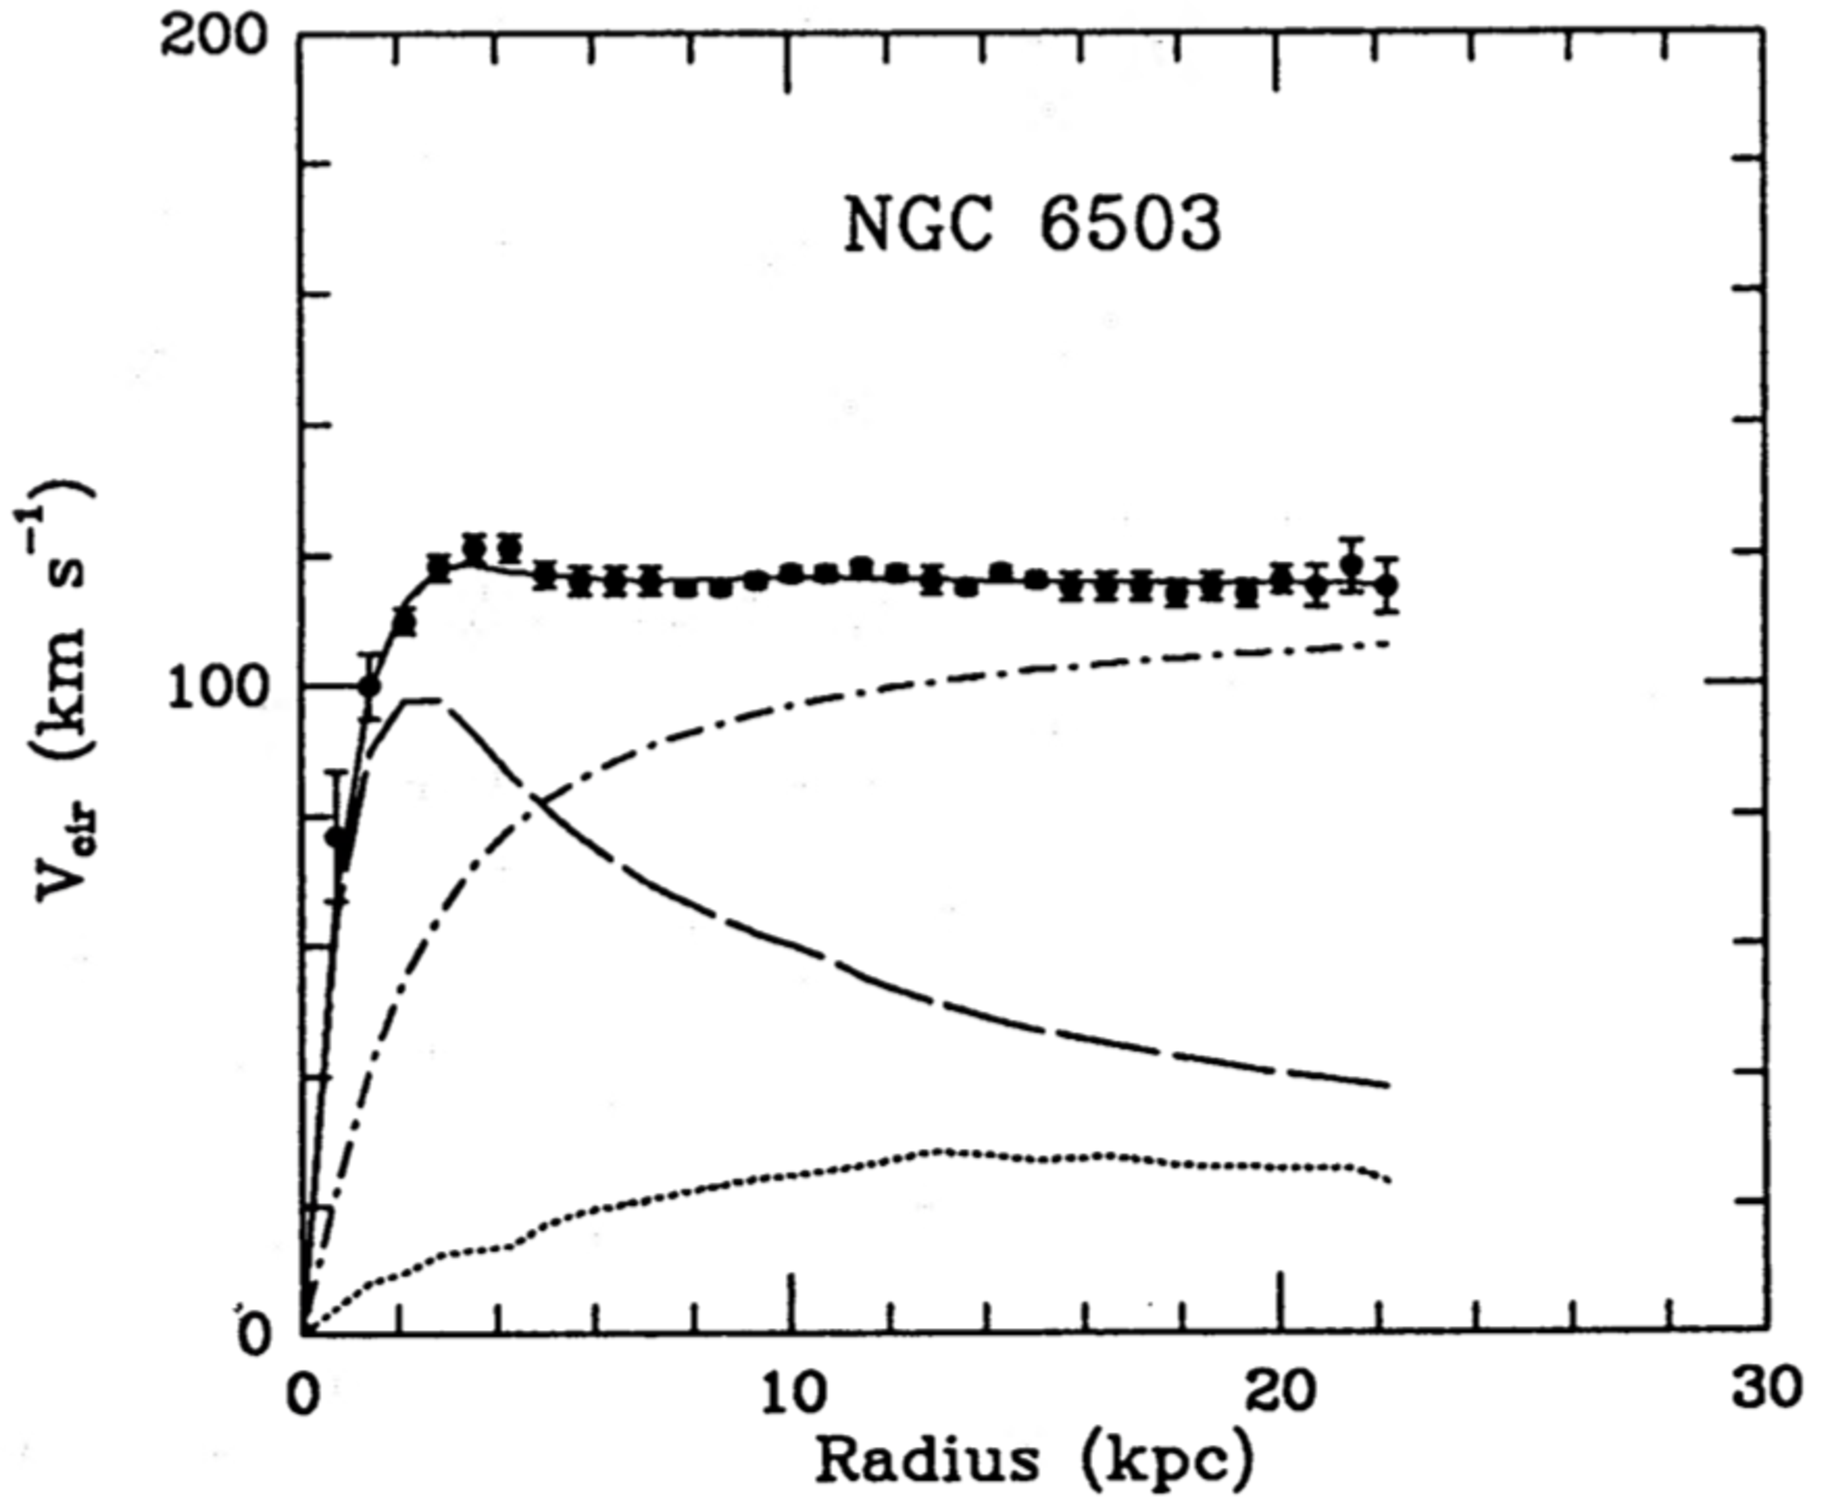
\includegraphics[height=5cm]{ngc_6503}}
  \end{subfloatrow}
  \hspace*{\columnsep}
  \begin{subfloatrow}
\vbox to 5.3cm{
  \ffigbox[\FBwidth]{\caption{}}
  {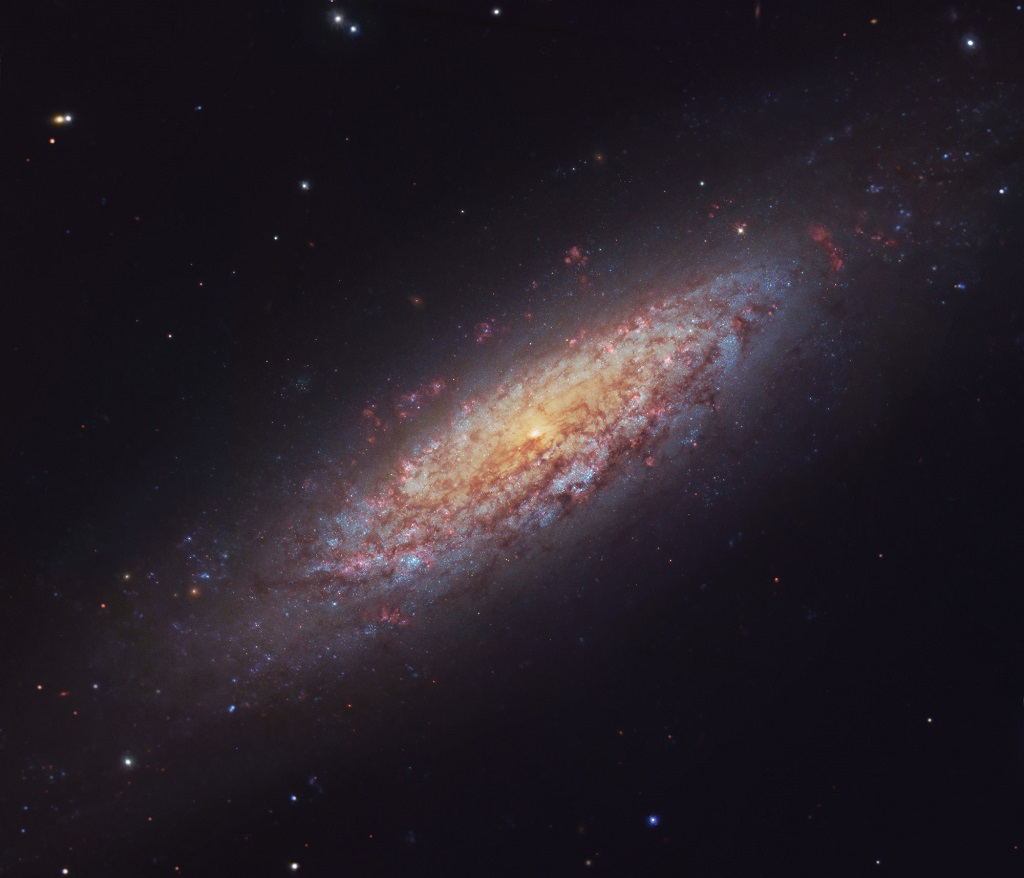
\includegraphics[trim={2cm, 2cm, 2cm, 2cm}, clip, height=4.4cm]{ngc_6503_image}}
}
  \end{subfloatrow}
  }{
  \vspace*{-10mm}
  \caption{Rotational velocity vs. radius (left) and image (right) of galaxy NGC 6503.  In the left panel visible components are
  represented by the dashed line, gas by the dotted, and dark halo by the dashed-dotted.
Image credit: (left) \citeref{Begeman1991}, (right) \citeref{Gendler2018}.}
	\label{fig:ngc_6501}
  }
\end{figure}

%for figure trim info
%https://tex.stackexchange.com/questions/57418/crop-an-inserted-image





\begin{figure}
	\centering
	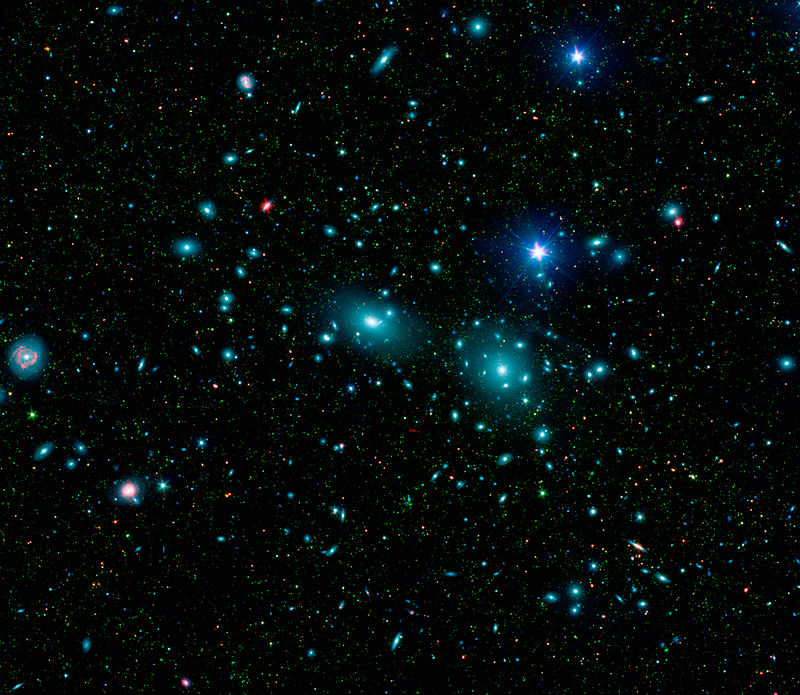
\includegraphics[width=0.5\textwidth]{coma_cluster}
	\label{fig:coma_cluster}
	\caption{Coma Cluster as seen by Sloan Digital Sky Survey and Spitzer Space Telescope.  Image credit: \citeref{NASA2018}.}
\end{figure}


%========
\subsection{Big Bang Nucleosynthesis}



%========
\subsection{Gravitational Lensing}
\label{subsec:gravitational_lensing}
A collection of matter capable of bending electromagnetic radiation between a source and an observer is a gravitational
lens.  The deflection is caused by the matter's gravitational distortion of space-time, for
the effects are typically most noticeable for high-density objects
such as galaxies, galaxy clusters, or stars.  The position of a source that is gravitationally lensed as viewed by an observer will be
incorrect, as shown in the right panel of \figref{fig:lensing}.  A lens can be characterized in part by its convergence
$\kappa$, which describes the focusing of the the light rays, and shear $\gamma$, which characterizes the image's ellipticity.  They can
are related to the magnification by

\begin{equation}
\mu = \frac{1}{(1-\kappa)^{2} + \gamma^{2}}
\end{equation}

\noindent and produces an increase in brightness when the source and lens are close to one another.  This amplification has helped
astronomers see objects that previously were thought to be too faint to observe.

In the case of strong lensing an observer will see a misshapen source as arcs.  Because the magnitude of the
deflection depends on the proximity to the lens, it is possible to see multiple instances of the same source.  In most cases the images
travel different distances so the observer will see different eras in the source's past.  In the special case
when the lens is directly between the source and observer the image will appear as a circular distortion of the source around the lens,
known as an Einstein ring, and no time delay will occur.  \figref{fig:lensing}
shows a photo of a strong lens and a diagram depicting the path of the light.  Originally Einstein
believed gravitational lensing was useless having only considered what today is known as micro lensing (deflection
about a star), but Fritz Zwicky predicted galaxies could provide stronger lensing and
magnification.  When the arcs have a suitable size and flux the source's luminosity can be determined.

\begin{figure}
 \centering
 \begin{subfigure}[t]{0.5\textwidth}
  \centering
  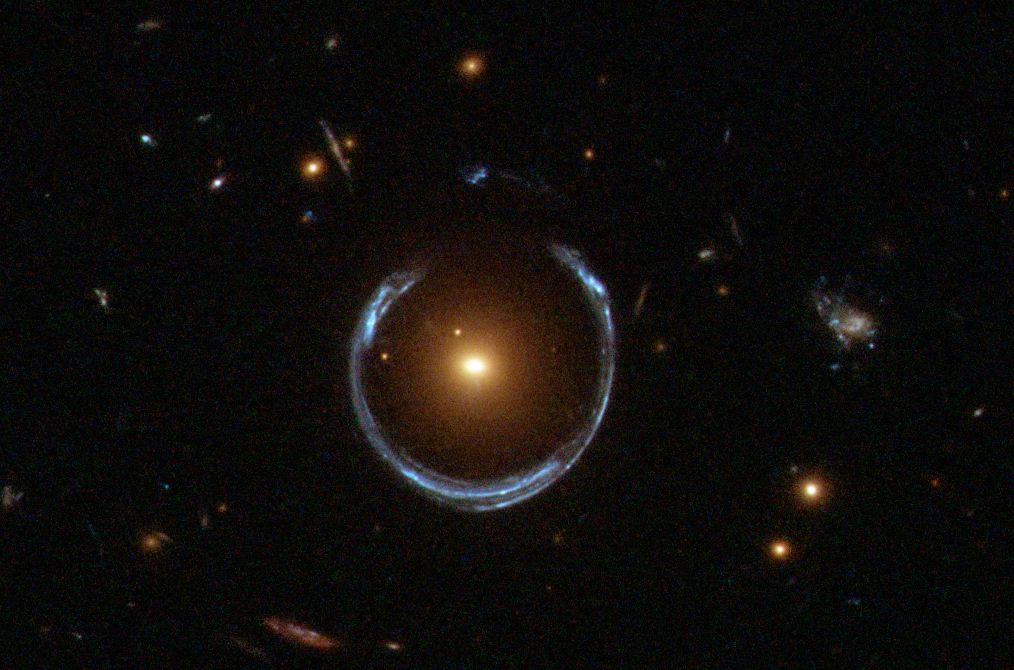
\includegraphics[trim={0cm, 2cm, 0cm, 0cm}, clip, height=4.5cm]{lensing_horseshoe}
 \end{subfigure}%
 \begin{subfigure}[t]{0.5\textwidth}
  \centering
  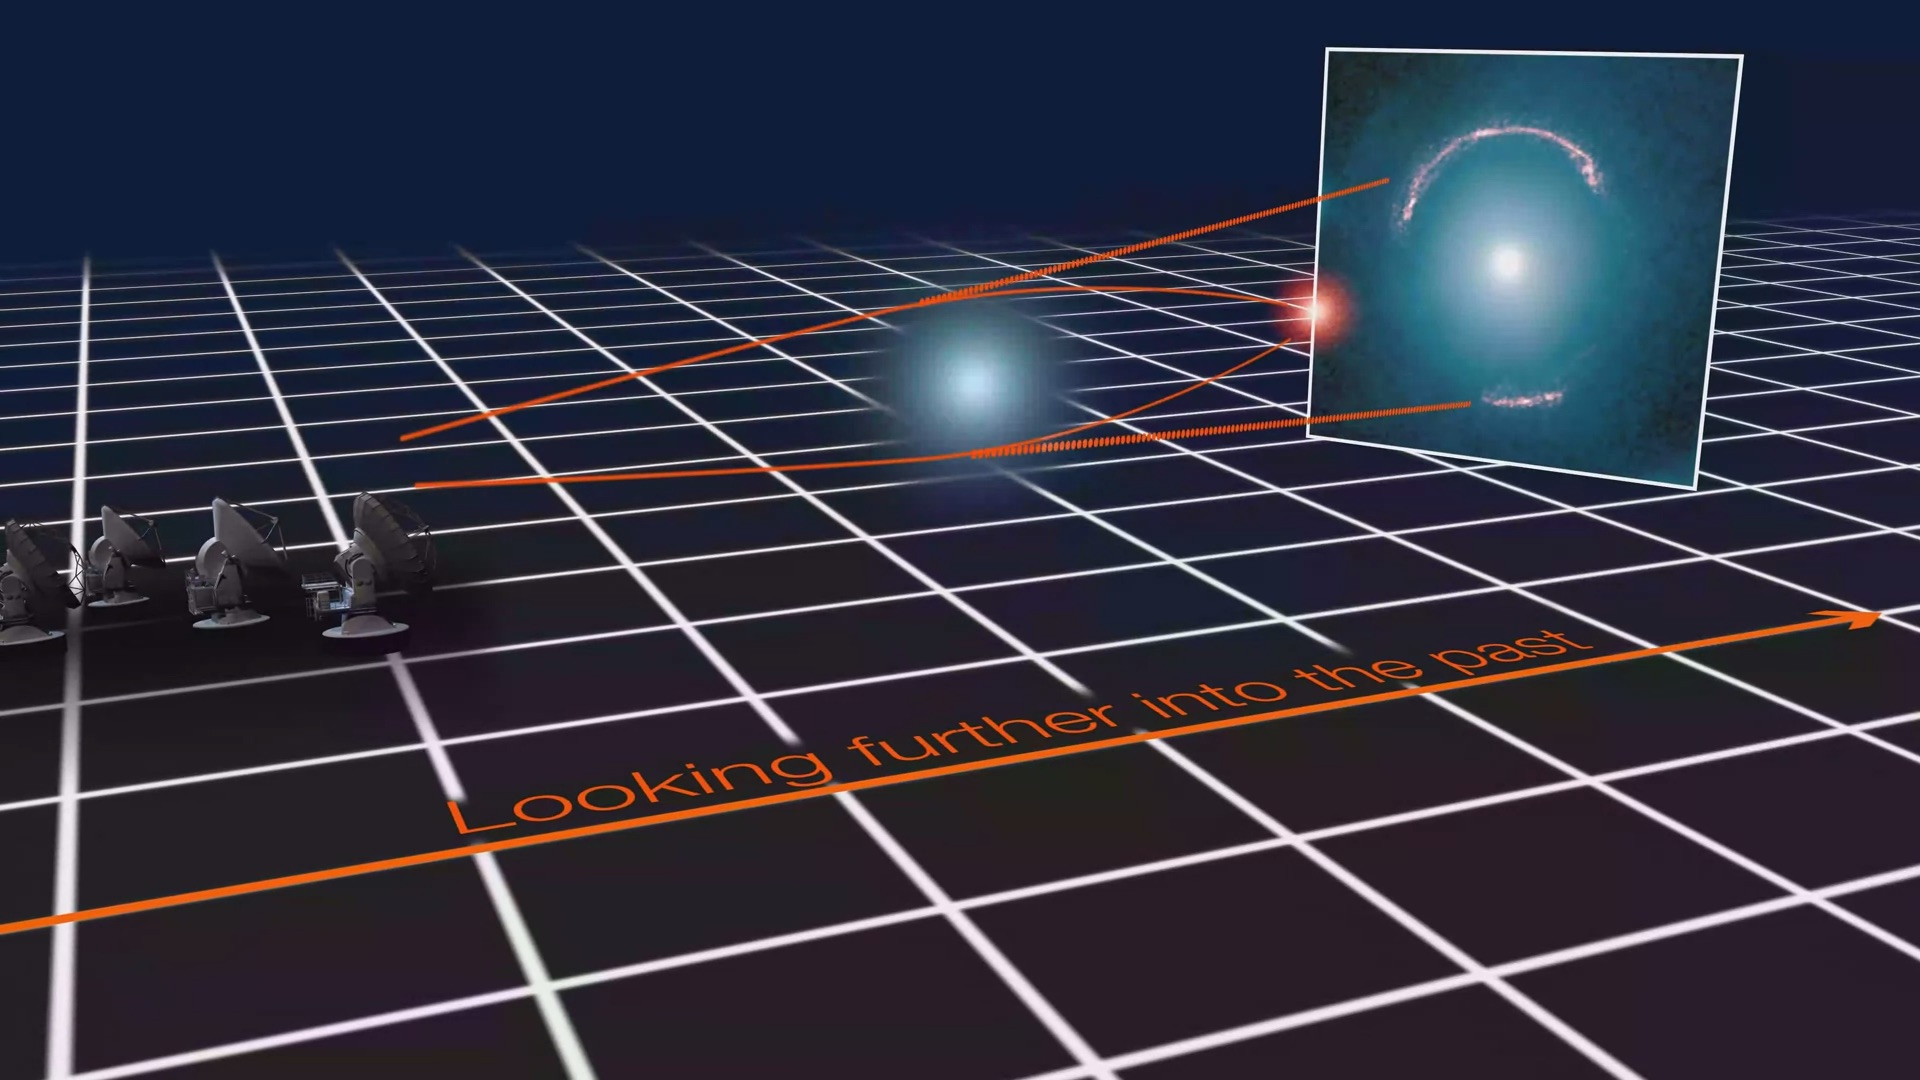
\includegraphics[trim={6cm, 0cm, 0cm, 0cm}, clip, height=4.5cm]{lensing_diagram}
 \end{subfigure}
 \caption{(left) A red galaxy distorts the light from a more distant blue galaxy to produce an Einstein ``horseshoe" ring.  (right)
 A diagram of strong lensing.  The red source is bent by the blue lens, with the solid orange lines that connect
 to it representing the light's true trajectory.  The observer incorrectly views the source's
 position as indicated by the dashed orange lines, and the image behind them.  Image credit: (left) \citeref{ESAHubbleNASA2018}, (right)
 \citeref{ESO2018}.}
 \label{fig:lensing}
\end{figure}


In many astrophysical instances the light's deflection is much more subtle.  This is known as weak
lensing, and because its effects are fainter is more difficult to observe.  Whereas strong lensing results from radiation passing around
the lens, weak lensing is the passage of light through a gravitational field where tidal effects distort the shape of the image.  In the
latter the luminosity is often too low for a thorough analysis so
astronomers may only consider the source's shear.  However, because the size of the shear for weak lensing is small, systematic
effects from observation (e.g. atmosphere, instrument point spread function, noise, etc.) must be small and well
understood \citeref{Paolis2016}.  Furthermore,
because galaxies are generally elliptical, decoupling the true shape from the shear can be difficult to impossible.  Thus the
gravitational field is calculated statistically by randomly sampling galaxies from the known ellipticity distribution.  Since the
number of samples must equal the number of galaxies along the line of sight, this method is most effective when the number of galaxies is
large.

If the mass of the lens is well-known, the visible portion can be subtracted to yield its fraction of dark matter.  This can typically
be done for strong lenses as shown in \figref{fig:lensing} but is more difficult for weak.



\begin{figure}
    \centering
    \begin{subfigure}[t]{0.45\textwidth}
        \centering
        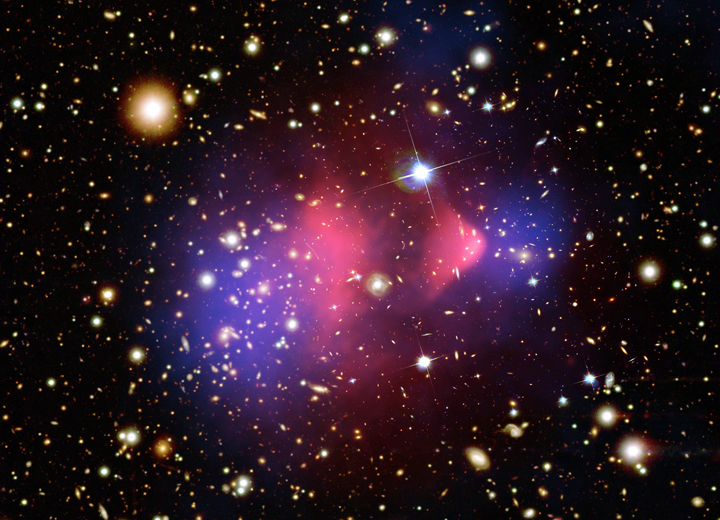
\includegraphics[height=4.5cm]{chandra_bullett_preview}
    \end{subfigure}%
    \begin{subfigure}[t]{0.45\textwidth}
        \centering
        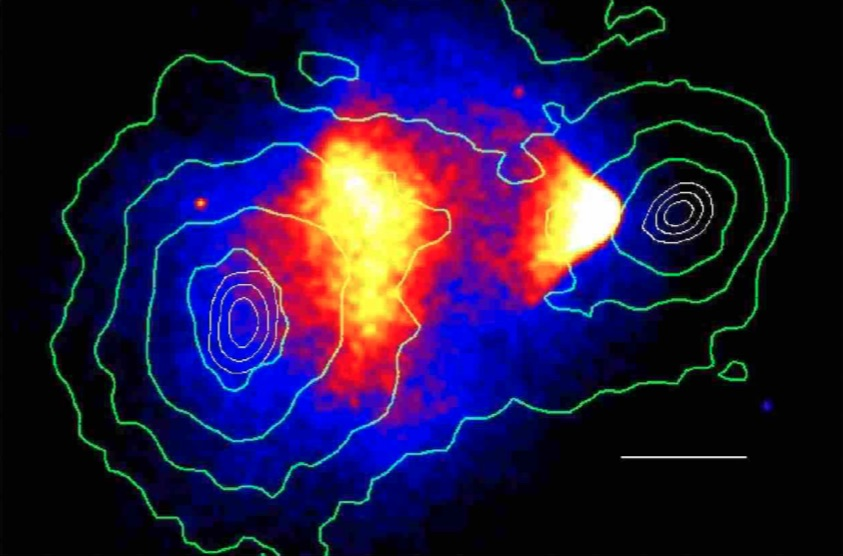
\includegraphics[height=4.5cm]{bullet_cluster_paper}
    \end{subfigure}
    \caption{X-ray emission from hot gas (pink) and mass centroids (blue) from gravitational lensing after
	collision of cluster 1E 0657-558.  The white bar in the right panel represents 200 kpc at cluster.  The separation
	between the colors provides evidence for Dark Matter.
	Image credit: (left) \citeref{Markevitch2006, Clowe2006}, NASA/CXC/CfA/STScIMagellan/U.Arizona/;
	Lensing Map: NASA/STScI; ESO WFI; Magellan/U.Arizona/D.Clowe et al. (right) \citeref{Clowe2006}.}
	\label{fig:bullet_cluster}
\end{figure}

A galaxy collision provides a unique setting to study dark matter.  1E0657-56, commonly known as the Bullet Cluster, is two galaxies that
passed through one another ${\sim}150$ million years ago at $4500_{-800}^{+1100}\ \mathrm{km\ s^{-1}}$
\citeref{Markevitch2004}.  \figref{fig:bullet_cluster} shows the x-ray map in pink and the mass
distribution from gravitational lensing measurements in blue in the left panel, and the mass contours in the right.  The separation of
mass from baryonic matter can be explained by dark matter.  As the galaxies collide intergalactic dust interacts
and heats up, creating x-rays and slowing their speed.  Because dark matter does not interact it passes
through affected only by gravity.  In addition to providing evidence of dark matter, 1E0657-56 sets a limit on the
cross-section of dark matter self-interaction of $<1\ \mathrm{cm^{2}\ g^{-1}}$ \citeref{Markevitch2004}.  It also provides evidence
against modified gravity (\secref{subsec:modified_gravity}) - an alternative theory to dark matter - since the observed mass distribution
are shown to lay outside of the luminous content.




%========
\subsection{Cosmic Microwave Background} \label{subsec:cmb}
The Cosmic Microwave Background (CMB) was accidentally discovered in 1965 by Arno Penzias and Robert Wilson, for which they received
the Nobel Prize \citeref{Penzias1965}.  It
is a remnant from shortly after (${\sim}380,000\ \mathrm{y}$, $z\sim1100$, $T\sim3000\ \mr{K}$) the Big Bang  and a near-perfect
blackbody at $2.725\ \mr{K}$ today (most precise measurement at $2.72548 \pm 0.00057\ \mr{K}$ \citeref{Fixsen2009}).  CMB photons
have been traveling freely since the time of last scattering $t_{\mathrm{ls}}$ - when electron-atom recombination in the early universe
was effectively complete, so photons ceased to scatter.

Deviations in the blackbody spectrum are small (root mean square of $\delta T/T \sim 10^{-5}$) and result from a number of
processes at $t_{\mathrm{ls}}$ that fluctuated throughout space.  A dipole anisotropy is due to
Earth's motion with respect to the comoving rest frame of the CMB \citeref{Smoot1991}.  Furthermore,
energy density perturbations would cause variations in gravitational potential $\delta \Phi$.  A
photon at a larger $\delta \Phi$ at $t_{\mathrm{ls}}$ would be blueshifted since as it moves its
potential decreases, while one at lower $\delta \Phi$ would be redshifted.  This is known as the
Sachs-Wolfe effect \citeref{Sachs1967}.  Details of additional effects, including intrinsic fluctuations and acoustic
oscillations, can be found in \citeref{Dodelson2003}.

\begin{figure}
\centering
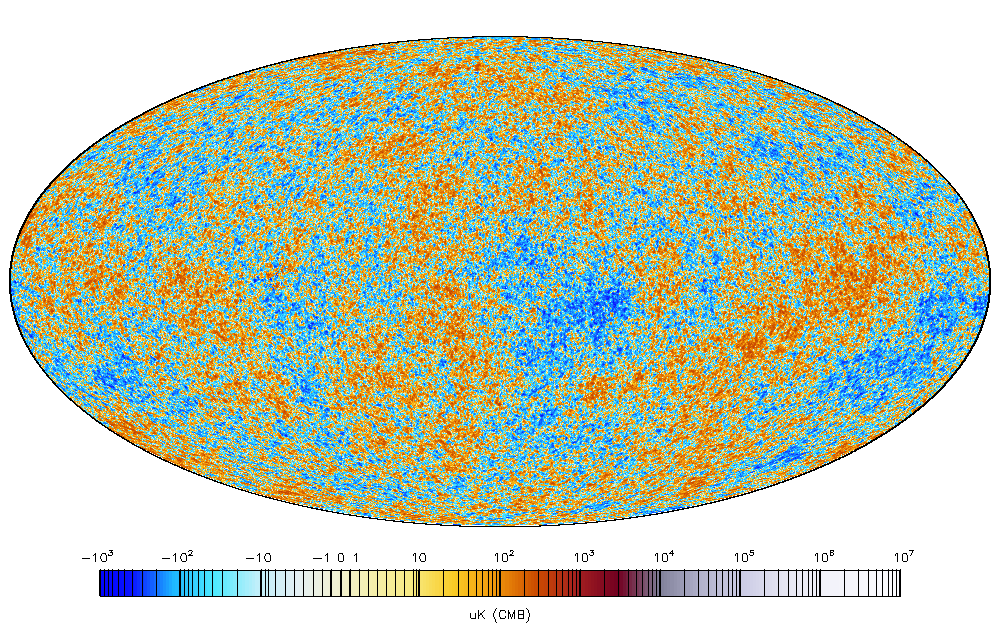
\includegraphics[width=0.8\textwidth]{PlanckFig_map_columbi1_IDL_HighDR_colbar_1000px_CMB_moll}
\caption{CMB as observed by Planck.  Temperature deviations $\delta T/T \sim 10^{-5}$.  Image credit: \citeref{}}
\label{fig:planck_map}
\end{figure}


The CMB provides the most precise measurements on numerous cosmological parameters including $\Omega_{\mathrm{b}}$,
$\Omega_{\mathrm{dm}}$, $\Omega_{\Lambda}$, $\Omega_{\mathrm{r}}$, and $H_{0}$.  It has been charted by several satellites since
its
discovery, most recently with Planck \citeref{Plack2011}.  The CMB is shown in \figref{fig:planck_map},
where fluctuations are on the order of $10^{\pm 3} \mathrm{\mu K}$.  These fluctuations were caused by the
amount of each component - thus, by calculating the correlation function

\begin{equation}
%C(\theta) = \Big \langle \frac{\delta T}{T}( \hat{n}) \frac{\delta T}{T} ( \hat{n}^\prime) \Big \rangle
C(\theta) = \Big \langle \delta T( \hat{n}) \delta T(\hat{n}^\prime) \Big \rangle
\label{eq:cmb_corr_func}
\end{equation}

\noindent we can identify the cosmological makeup of the universe.  To do this we use

\begin{equation}
\delta T = \sum\limits_{l=0}^{\infty} \sum\limits_{m=-l}^{l} a_{lm}Y_{lm}(\theta, \phi)
\label{eq:cmb_delta_t}
\end{equation}

\noindent where $\delta T = T(\theta, \phi) - \langle T \rangle$ for a given $\theta , \phi$
on the map.  $Y_{lm}(\theta, \phi)$ are the spherical harmonics with coefficients $a_{lm}$
such that $\sum\limits_{l,m} |a_{lm}|^{2} = 1$.  Substituting \eqnref{eq:cmb_delta_t} into \eqnref{eq:cmb_corr_func} gives a correlation
function of

\begin{equation}
C(\theta) = \frac{1}{4 \pi} \sum\limits_{l=0}^{\infty} (2l + 1) C_{l} P_{l}(cos \theta)
\end{equation}

\noindent where $P_{l}$ are the Legendre polynomials and $C_{l} = \frac{1}{2l + 1} \sum\limits_{m=-l}^{l} a_{lm}$.  The
only unknown is $C_{l}$, which is typically given as the angular power spectrum
$D_{l}^{TT} \equiv l(l+1)C_{l}/2\pi$ as shown in \figref{fig:cmb_power_spectrum}.

\begin{figure}
%	\centering
	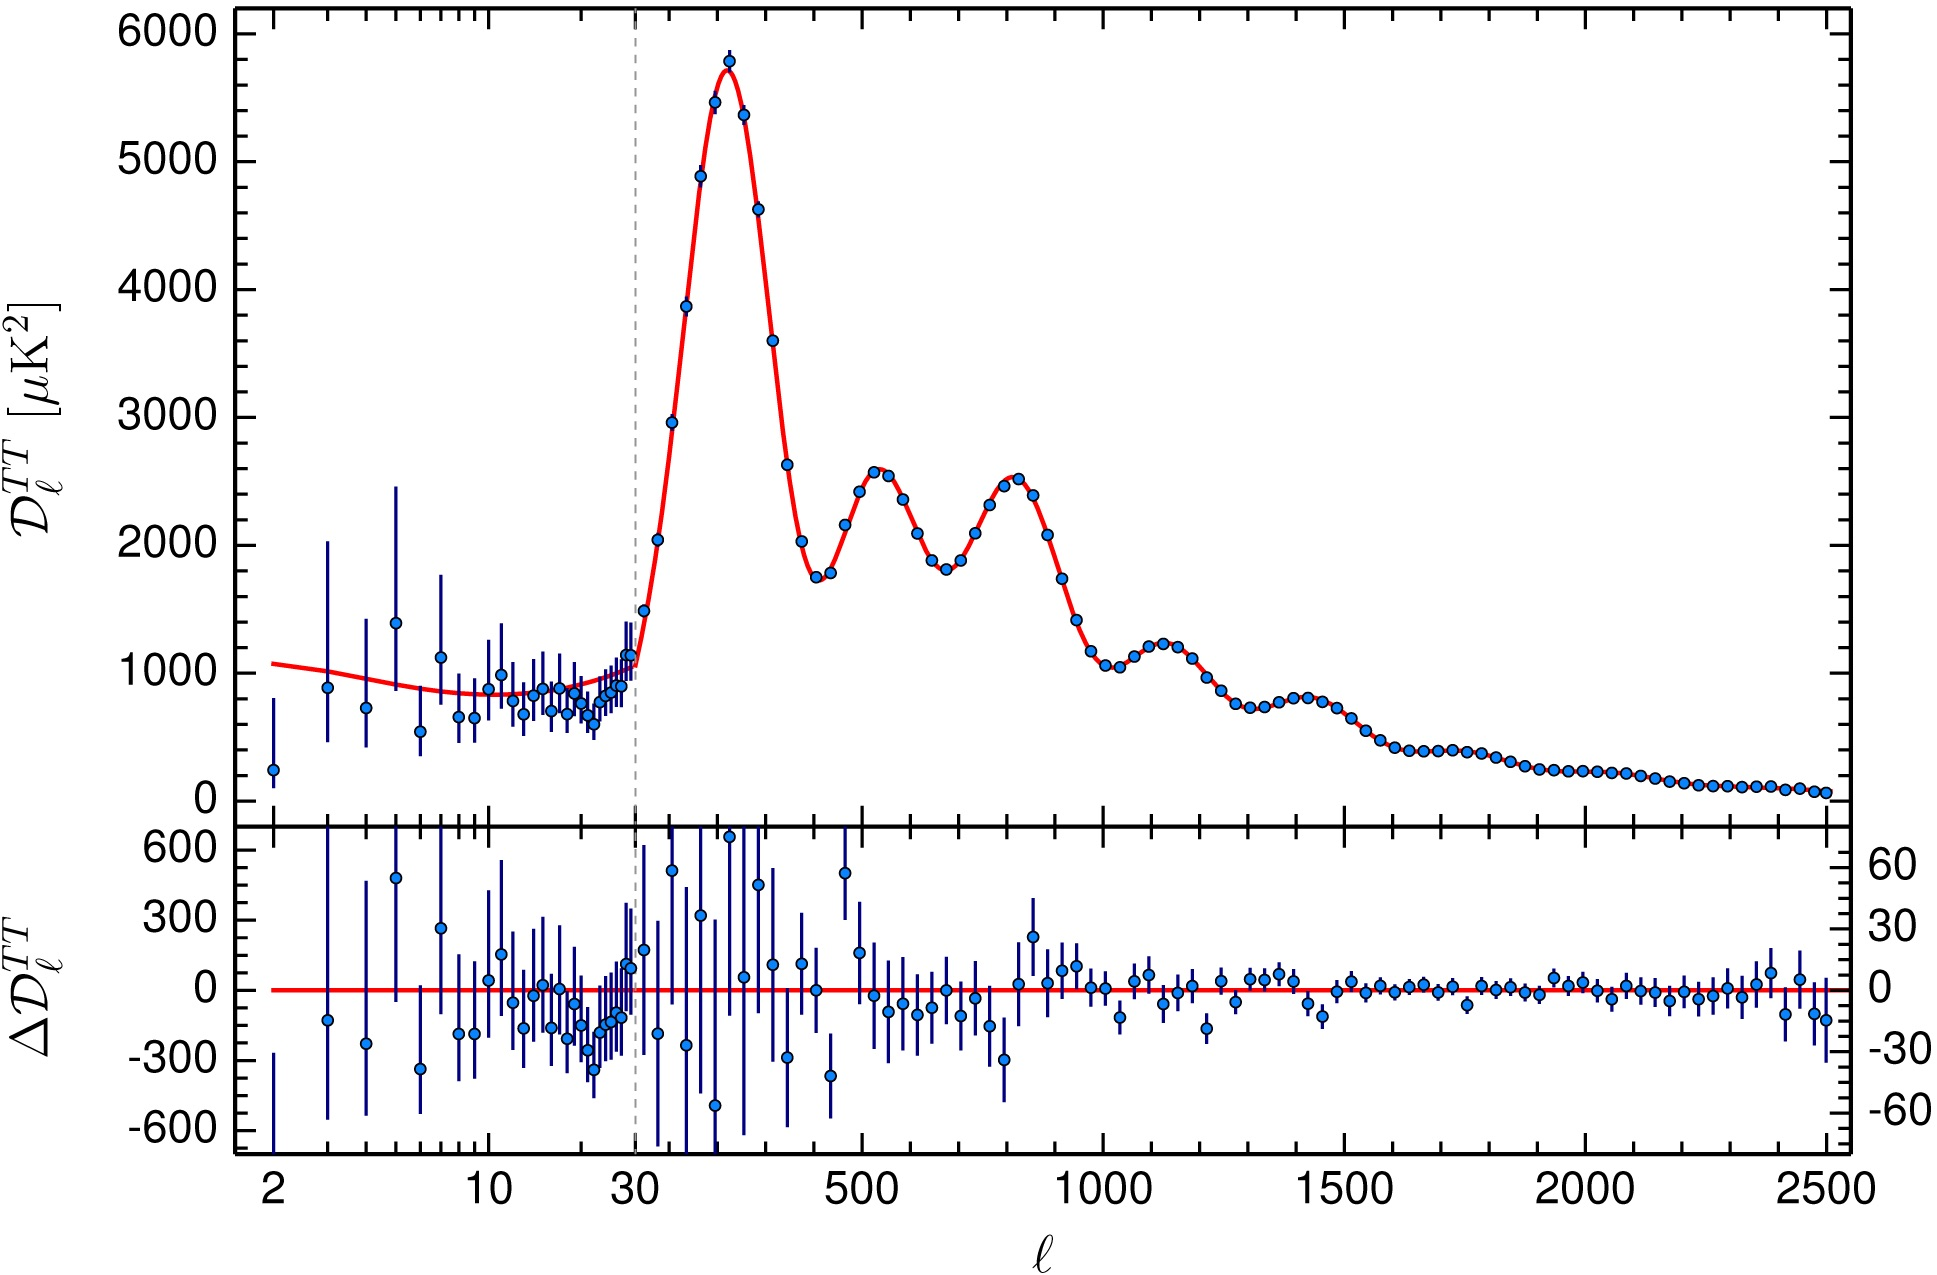
\includegraphics[width=0.8\textwidth]{cmb_power_spectrum}
	\centering
	\caption{Angular power spectrum for CMB from Planck fit using the $\Lambda$CDM model.  Residuals
	are shown in bottom panel.  The model matches the data well at $l < 15$ and $l > 30$.  The horizontal axis changes from linear to
	logarithmic at $l = 29$ and is marked by vertical dashed grey
	line. Image credit: \citeref{Planck2016}.}
	\label{fig:cmb_power_spectrum}
\end{figure}

Details about cosmological parameters including $\Omega_i$ are contained in the angular power spectrum (e.g. information on the curvature
is found in the first peak while the $\Omega_{\mathrm{b}}$ is derived from the ratio of the heights of the first two peaks).  The results
of the fit give $H_{0} = 67.81 \pm 0.92\ \mathrm{km\ s^{-1}\ Mpc^{-1}}$, $\Omega_{\Lambda} = 0.692 \pm 0.012$,
$\Omega_{\mathrm{b}} = 0.0484 \pm 0.0005$, $\Omega_{\mathrm{dm}} = 0.258 \pm 0.004$, and curvature density parameter
$\Omega_{k} \equiv 1 - \Omega_{\Lambda} - \Omega_{\mathrm{b}} - \Omega_{\mathrm{dm}} =  -0.005_{-0.017}^{+0.016}$.


%[5] Adams, F.C., Freese, K. & Guth, A.H. [1991], Phys. Rev. D43, 965.



%$\Omega_{m} = 0.308 \pm 0.012$
%$H_{0} = 67.81 \pm 0.92$
%$\Omega_{\Lambda} = 0.692 \pm 0.012$
%$\Omega_{b}h^{2} = 0.02226 \pm 0.00023$
%$\Omega_{c}h^{2} = 0.1186 \pm 0.0020$
%$N_{eff} = 3.046$
%$\Omega_{k} \equiv 1 - \Omega_{m} - \Omega_{\Lambda} = -0.005_{0.017}^{0.16}$ for $\Lambda CDM$

%========
%\subsection{Structure Formation} \label{subsec:structure}

%\endcsname

%====================================
\section[Dark Matter Candidates][Dark Matter Candidates]{Dark Matter Candidates}
\label{sec:dmcandidates}
Despite strong evidence for the existence of dark matter, there is little guidance for its composition.  Any dark matter candidate must
have a lifetime much larger than the age of the universe, be electrically
neutral, and have a small matter-dark matter cross section.  Of course, dark matter may constitute a class of particles so long as their
sum satisfies our observations of the universe.



\subsection{Modified Gravity}
\label{subsec:modified_gravity}
One possible explanation for the disparity between the mass of ordinary matter and its behavior is an incomplete understanding of
gravity.  This
would suggest that Einstein's General Relativity works well at small distances but does not correctly explain large-scale
gravitation.  Since the incompatibility of current theory with observation would be a resolved by proving the mysterious behavior is
a consequence of ordinary matter, dark matter would not be necessary.

Major evidence against modified gravity emerged in 2004 when the collision of two galaxies 1E0657-56 (Bullet Cluster) was observed
(\secref{subsec:gravitational_lensing}).  \citeref{Markevitch2004} reconstructed the mass distribution of the merger from gravitational
lensing measurements (\figref{fig:bullet_cluster}).  Their measurements required a significant fraction of the mass
distribution to be offset from the visible matter, consistent with collisionless dark matter halos passing through one another.  This
presented a problem for modified gravity, which was unable to justify this.

In 2018 the ultra-diffuse galaxy NGC1052-DF2 was observed to have $M_{\mathrm{halo}} / M_{\mathrm{stars}} \sim 1$, a factor of
roughly $400$
lower than expected \citeref{VanDokkum2018a, VanDokkum2018b}.  This poses a challenge to modified gravity - including modified Newtonian
dynamics
(MOND), a popular theory that has successfully predicted a number of galactic phenomena \citeref{Milgrom1983} - since a large
gravitational
field does not appear to exist around the baryonic matter.  However, several theories have claimed this may be compatible with their
expectations due to its proximity to its massive host galaxy NGC1052 and large uncertainties on some of the measurements by
\citeref{VanDokkum2018a, Famaey2018, Moffat2018}.  Under the dark matter hypothesis, a galaxy without DM has implications outside
this field - e.g. current models of structure formation cannot explain this \citeref{Abraham2018, Ogiya2018}.  Two recent
papers found conflicting results when studying the 175 SPARC
galaxies \citeref{Lelli2016}.  The first was in agreement with MOND using gaussian priors centered around values given by SPARC by
setting
their uncertainty to observational errors \citeref{Li2018}.  The second included an additional 18 galaxies from THINGS
\citeref{deBlok2008} and with flat priors excluded MOND
at $10 \sigma$ \citeref{Rodrigues2018}.  Ultimately additional measurements and improved statistics are needed to better
quantify NGC1052-DF2, but confirmation of missing dark matter would strongly constrain theories of modified gravity.



%========
\subsection{Axions} \label{subsec:axions}
Charge conjugation and parity (CP) violation in strong interactions has never been observed, despite its prediction
by quantum chromodynamics (QCD).  This compels a theoretically unjustified fine tuning of the model, which
is known as the strong CP problem.  Originally hypothesized by Roberto Peccei and Helen Quinn in 1977, the
axion - a new standard model particle - offered a solution \citeref{Peccei1977}.  Shortly after it was
demonstrated that for an axion decay constant of $f_{\mathrm{a}} > 10^{12}$ axions would be overproduced in the
early universe and cause the axion density $\Omega_{\mathrm{a}} > 1 > \Omega_{\mathrm{dm}}$ \citeref{Preskill1983}.  However, if the
decay constant were ${\sim} 10^{12}$ the axion density could be equivalent to $\Omega_{\mathrm{dm}}$.  Current mechanisms for solving
the strong CP problem rely on invisible axion models Kim-Shifman-Vainshtein-Zakharov (KSVZ) \citeref{Kim1979, Shifman1980} and
Dine-Fischler-Srednicki-Zhitnitsky
(DFSZ) \citeref{Zhitnitsky1980, Dine1981}, marked along the yellow band in \figref{fig:axions}.  $f_{\mathrm{a}}$ is inversely
proportional to the axion mass $m_{\mathrm{a}}$.

\begin{figure}
\centering
\includegraphics[width=\textwidth]{axion_limits}
\caption{Axion-double photon coupling with respect to mass.  The shaded regions have been excluded by different experiments.  Invisible
axion models KSVZ and DFSZ are drawn along the yellow band.  Image credit: \citeref{Patrignani2016}.}
\label{fig:axions}
\end{figure}

%The axion
%mass $m_{a} = 57(10^{11}GeV/f_{a})\ \mu$eV, which gives a lower bound of $m_{a} \sim 5\ \mu$eV.

Because axions naturally offer an explanation for dark matter there are a number of DM experiments dedicated to
finding them.  Several operate under the Primakoff effect \citeref{Primakoff1951}, which states that electromagnetic fields should
transform
axions to photons and vice versa.  Cavity searches such as the Axion Dark Matter Experiment (ADMX) \citeref{ADMX2018} search the galactic
dark matter halo using a resonant microwave cavity inside a superconducting magnet
to convert axions into microwaves.  Others, like the CERN Axion Solar Telescope (CAST) search for axions produced in the Sun's
core via x-ray scattering off of protons and electrons.  The experiment would convert solar axions back into x-rays.  The Cosmic Axion
Spin Precession Experiment (CASPEr) uses nuclear magnetic resonance (NMR) to detect nuclear spin precession frequencies that depend on
$m_{\mathrm{a}}$ \citeref{CASPEr2018}.  In addition axion-induced electronic recoils have been searched for in cryogenic detectors
including CDMS \citeref{CDMS2009}, EDELWEISS \citeref{EDELWEISS2013}, and XMASS \citeref{XMASS2013}.  The best coupling limits to
date were set by XENON100 in 2014 \citeref{Aprile2014}.


%========
\subsection{WIMPs} \label{subsec:wimps}
Weakly Interacting Massive Particles (WIMPs) are another favored candidate for dark matter.  As their name
suggests, they interact through the weak force so would be difficult to observe.  They
would behave similarly to neutrinos, which have a small cross-section and interact only via the weak force.  They must also have been
produced early in the universe to account for observations of the CMB and galactic structures.

At the beginning of the universe the temperature was hot enough where particles could annihilate with their
antiparticle counterpart and produce new particles, maintaining equilibrium.  As the universe cooled each
particle had a ``freeze-out", when they could no longer transform freely to other particles.  Using the
$\Lambda$CDM model the density of DM in the universe today is given by

\begin{equation}
\Omega_{\mathrm{dm}}h^{2} = \frac{3 \times 10^{-27}\ \mathrm{cm^{3}\ s^{-1}}}{\langle \sigma_{\mathrm{ann}} v \rangle}
\end{equation}

\noindent where $h \equiv H_0 / 100$ and $\langle \sigma_{\mathrm{ann}} v \rangle$ is
the thermally averaged self-annihilation cross section
for dark matter.  Assuming DM has a cross-section and mass on the order of the weak scale,
it would give roughly the correct relic density of DM.  This is known as the ``WIMP miracle".

Another appealing argument for WIMPs is supersymmetry (SUSY), which is theorized to solve a number of problems
in the standard model.  Many SUSY models predict a heavy stable particle that would be weakly interacting (a favorite is the neutralino,
the supersymmetric partner of the neutrino).  This has historically been one of the favored arguments for WIMP dark matter.

%========
\subsection{Cold, Warm, or Hot} \label{subsec:hot_vs_cold}
An important property of dark is whether it was relativistic in the early universe, typically defined using the times of decoupling from
other components $t_{\mathrm{dec}}$ and matter-radiation equality (moment when density of matter and radiation are equivalent)
$t_{\mathrm{rm}}$.  Hot dark matter (HDM) would have been relativistic at $t_{\mathrm{dec}}$ and $t_{\mathrm{rm}}$.  Warm dark matter
(WDM) would have been relativistic at $t_{\mathrm{dec}}$
but not at $t_{\mathrm{rm}}$.  Cold dark matter (CDM) would have been non-relativistic at both.  Candidates for CDM include
WIMPs, axions, and primordial black holes while for WDM might be the gravitino.  Neutrinos are candidates for both
warm and hot dark matter, but measurements show their density is orders of magnitude to small to account for $\Omega_{\mathrm{df}}$.

Structure formation in the universe unravels the hot/warm/cold dark matter mystery.  Because the cosmological layout we observe
today came from fluctuations in the earliest moments of the Big Bang (\secref{subsec:cmb}) the structure
contains the imprint of dark matter.

In hot dark matter relativistic DM would smooth out density perturbations, in what is known as free
streaming.  In this case the first structures to form would be superclusters, followed by smaller-scale
features.  Observations show that this is not the case; galaxies have been around since before the universe
was 1 billion years old ($z \sim 6$) and superclusters are just forming today \citeref{Ryden2003}.

CDM allows early density perturbations to persist, causing smaller structures to materialize first,
consistent with galaxy surveys between ${\sim} 1$ Mpc to the cosmological horizon.  At scales $< 1$ Mpc and
$M \sim 10^{11} \ M_{\odot}$ there are discrepancies, including under-dense cores for many galaxies that are DM-dominated
and significantly fewer satellite dwarf and small galaxies than predicted \citeref{Moore1999, Klypin1999}.  Possible
solutions to the latter may be that dwarf galaxies have merged, been stripped by tidal forces of larger galaxies, or
not accumulated enough baryonic matter to be visible \citeref{Simon2007}.

WDM has received a lot of interest since the problems with CDM were discovered.  Simulations have shown that
WDM would result in fewer subhalos, though explaining the other CDM model-observation disagreements has been less
successful \citeref{Bullock2017, Ogiya2017}.  However, because neutrinos have mass there
was at least some non-CDM in the early universe.

Despite problems with CDM it remains the most favorable model for dark matter.  One possible outcome is
there is a mix of CDM and WDM, but if that's the case CDM would make up the considerable bulk of dark matter.


%====================================
\section[WIMP Detection Methods][WIMP Detection Methods]{WIMP Detection Methods}
\label{sec:detection}

There are three methods for detecting WIMPs.  The first is using particle colliders where standard model (SM) particles would interact and
create DM (\secref{subsec:colliders}).  The second is via indirect detection, where DM would annihilate into SM particles, with the hope
that they would be detectable
on Earth (\secref{subsec:indirect}).  The third method is by means of direct detection in which DM would scatter off SM matter, producing
a signal that could be
observed (\secref{subsec:direct}).  These methods are outlined in \figref{fig:detection_methods}.

\begin{figure}
\centering
\includegraphics[width=0.8\textwidth]{}
\caption{Detection Methods.}
\label{fig:detection_methods}
\end{figure}

 %========
\subsection{Colliders} \label{subsec:colliders}
One mechanism through which we might observe WIMP dark matter is through particle-antiparticle
annihilation.  This could be observed at particle colliders where energies can exceed
several TeV, producing dark matter particle-antiparticle pairs that
would escape undetected.  This could be measured from momentum conservation where there would be missing transverse energy (MET).  The
Large Hadron Collider (LHC) is investigating the quark sector with energies
exceeding 10 TeV, while the Large Electron-Positron (LEP) Collider is doing so for leptons at
${\sim} 200$ GeV.  Both experiments are competitive at lower energies than noble gas experiments (\secref{subsec:noble_gas}), particularly
for spin-dependent searches \citeref{Fox2011, Alpigiani2017}.  Annihilation alone would not prove the discovery of dark matter but would
need
indirect or direct experiments to validate their results.  However, it would still be extremely useful in narrowing the search region.

\begin{figure}
\centering
\includegraphics[width=0.8\textwidth]{collider_diagram}
\caption{Diagram of a collision at the LHC.  Image credit: \citeref{CERN2018}.}
\label{fig:collider}
\end{figure}


 %========
\subsection{Indirect Detection} \label{subsec:indirect}
Indirect detection looks for signatures of dark matter by observing standard model particles.  Such observables
may come from dark matter annihilation, wherein two DM particles annihilate and produce standard model
gamma rays or other particle-antiparticle pairs.  Alternatively, if DM is unstable (albeit with very long half-life) it may decay into
standard model particles that can be detected.

Indirect experiments look at regions where they expect a large number of interactions.  The local
dark matter density is estimated to be 0.2-0.56 GeV cm$^{-3}$ \citeref{Read2014} and experiments are observing
the Sun hoping to measure a WIMP-induced high energy neutrino flux \citeref{Ellis1988}.  Other theories suspect
DM annihilation in the galactic halo would produce
antiprotons, positrons, and gamma rays that would be detectable from Earth.  Because the galaxy's center
has a large flux of cosmic rays it is difficult to distinguish dark matter from other astrophysical
sources.  Nearby (${\sim} 50$ kpc) dwarf spherical
galaxies have become an attractive target where star formation regions have low $\gamma$-ray backgrounds \citeref{Zitzer2016}.

$\gamma$-rays need to be measured space because for the necessary energy range (GeV to TeV) photons interact
with matter via $e^{+}e^{-}$ pair production (\figref{fig:phot_atten}), so would be unable to pass through Earth's atmosphere.  However,
they can look for signatures such as showers of secondary particles and their Cerenkov
light as they pass through the atmosphere \citeref{Bertone2005}.

% for Ellis1988 reference listed above get their references 6 and 7 and maybe 8 for citations, need access to PRL


 %========
\subsection{Direct Detection} \label{subsec:direct}
Direct detection looks for low energy (${\sim} 1 \mdash 100$ keV) nuclear recoil (somes theories predict DM-lepton
but here they are not discussed) \citeref{Kopp2009}.  It is common to assume the dark matter halo of a galaxy is an isothermal
single-component sphere with an isotropic Maxwell-Boltzmann velocity distribution function
($f(\vectlett{v}) \propto \mathrm{exp}(-|\vectlett{v}|^2 / v_0^2)$) \citeref{Bhattacharjee2013}, though there is not a consensus on
whether this is the correct velocity parameterization
\citeref{Diemand2004, Kuhlen2009}.  This is known as the Standard Halo Model (SHM).  Given that the majority of dark matter must be
non-relativistic (\secref{subsec:hot_vs_cold}), we can calculate the differential recoil spectrum as \citeref{Undagoitia2016}

\begin{equation} \label{eq:dr_de}
\frac{dR}{dE}(E, t) = \frac{\rho_{0}}{m_{\chi}m_{\mathrm{A}}} \int_{v_{\mathrm{min}}}^{v_{\mathrm{esc}}}
v f(\vectlett{v}, t) \frac{d\sigma}{dE}(E, t)\ d^{3}\vectlett{v}
\end{equation}

\noindent where $\rho_{0} = 0.2 \mdash 0.56\ \mathrm{GeV\ cm^{-3}}$ is the local dark matter density (\secref{subsec:indirect}),
$m_{\chi}$ is the mass of a
dark matter particle, $m_{\mathrm{A}}$ is the mass of the target element, $v_{\mathrm{esc}}= 533_{-41}^{+54}\ \mathrm{km\ s^{-1}}$
\citeref{Piffl2014} is the escape velocity for WIMPs from the
galaxy, $f(\vectlett{v}, t)$ is the local velocity dispersion, and $\frac{d\sigma}{dE}(E, t)$ is the nucleon-DM differential
cross-section.  $v$ is the velocity of the dark matter in the rest frame of the detector.  The minimum velocity that will produce
a recoil of energy E is given by

\begin{equation}
v_{\mathrm{min}} = \sqrt{\frac{m_{\mathrm{A}} E}{2 \mu^{2}}}
\end{equation}

\noindent where $\mu_{\mathrm{A}} = m_{\mathrm{A}} m_{\chi} /( m_{\mathrm{A}} + m_{\chi})$ is the reduced WIMP-nucleus mass.

For WIMP searches most experiments
are looking at spin-independent (SI) or spin-dependent (SD) interactions.  For spin-independent all nucleons
contribute equally.  For spin-dependent, atoms must have an odd number
of protons or neutrons since only unpaired nucleons contribute to the search.  The differential cross-section can then be written as

\begin{equation} \label{eq:diff_sigma_si}
\frac{d \sigma}{dE} = \frac{m_{\mathrm{A}}}{2 \mu_{\mathrm{A}}^{2} v^{2}} \big( \sigma_{\mathrm{SI}}^{(0)} F_{\mathrm{SI}}^{2}(E) +
\sigma_{\mathrm{SD}}^{(0)} F_{\mathrm{SD}}^{2}(E) \big)
\end{equation}

\noindent where $\sigma_{\mathrm{SI}}^{(0)}$ and $\sigma_{\mathrm{SD}}^{(0)}$ are the cross sections at zero momentum for
spin-independent and spin-dependent DM.  $F_{\mathrm{SI}}^{2}(E)$ and $F_{\mathrm{SD}}^{2}(E)$ are the form factors, which
account for the cross section's decrease with increasing energy \citeref{Lewin1996}.  Spin-dependence is no longer discussed but details
are found in \citeref{Lewin1996}.  The SI form factor is
the Fourier transform of the mass density ground state, and for the parameterization given in \citeref{Helm1956} is given by

\begin{equation}
F_{\mathrm{SI}} = \frac{3 j_{1}(qr_{\mathrm{n}})}{qr_{\mathrm{n}}} e^{-(qs)^{2}/2}
\end{equation}

\noindent where $j_1(q r_{\mathrm{n}})$ is a Bessel function of the first kind, $q = \sqrt{2m_{\mathrm{A}}E}$ is the momentum,
$r_{\mathrm{n}} = \sqrt{1.2A^{2/3} - 5s^{2}}$, and $s \sim 1$ fm is a measure of the nuclear skin \citeref{Lewin1996, Engel1991}.  The
cross section is given by

\begin{equation} \label{eq:sigma_si}
\sigma_{\mathrm{SI}}^{(0)} = \sigma_{\mathrm{p}} \frac{\mu_{\mathrm{A}}^{2}}{\mu_{\mathrm{p}}^{2}} \frac{\big[ Z f_{\mathrm{p}} +
(A - Z) f_{\mathrm{n}} \big]^{2}}{(f_{\mathrm{p}})^{2}}
\end{equation}

\noindent where $\sigma_{\mathrm{p}}$ is the cross section of a proton Z is the number of protons and $\mu_{\mathrm{p}}$ is
the WIMP-nucleon reduced mass. $f_{\mathrm{p/n}}$ is the coupling strength for protons and neutrons, which are assumed to be
equivalent (see \citeref{Yaguna2017} for $f_{\mathrm{p}} \neq f_{\mathrm{n}}$).  Substituting \eqnref{eq:sigma_si} into
\eqnref{eq:diff_sigma_si} gives a spin-independent differential cross-section of

\begin{equation}
\frac{d \sigma}{dE} = \frac{m_{\mathrm{A}} \sigma_{\mathrm{p}}}{2 \mu_{\mathrm{p}}^{2} v^{2}}
 A^{2} \big| F(E) \big |^{2}
\end{equation}

\noindent This gives the differential rate as 

\begin{equation}
\frac{dR}{dE} = \frac{\rho_{0} A^{2} \sigma_{\mathrm{p}}}{2 m_{\mathrm{\chi}} \mu_{\mathrm{p}}^{2}}
  \big| F(E) \big |^{2} \int_{v_{\mathrm{min}}}^{v_{\mathrm{esc}}}
\frac{f(v)}{v}\ dv
\label{eq:dr_de_final}
\end{equation}

\noindent A direct detection experiment that is sensitive between energies $E_{\mathrm{min}}$ and $E_{\mathrm{max}}$ will measure
the number of signals over a time $T$ for their target mass $M$ as

\begin{equation} \label{eq:counts}
N ( m_{\chi}, \sigma) = T \times M \times \int_{E_{\mathrm{min}}}^{E_{\mathrm{max}}} \frac{dR}{dE} dE
\end{equation}

\noindent \eqnref{eq:dr_de_final} and \eqnref{eq:counts} state that the sensitivity of an experiment improves linearly with time and
target mass, but quadratically with $A$.  This makes the atoms of molecules of the target mass important consideration when
designing a direct detection experiment.

%For SD interactions the cross-section is

%\begin{equation}
%\sigma_{0}^{\mathrm{SD}} = \frac{32}{\pi} \mu_{\mathrm{A}}^{2} G_{\mathrm{F}}^{2} \big[ a_{\mathrm{p}} \langle S^{\mathrm{p}} \rangle +
%a_{\mathrm{n}} \langle S^{\mathrm{n}} \rangle \big] \frac{J + 1}{J}
%\end{equation}

%\noindent where $G_{\mathrm{F}}$ is the Ferm coupling constant, $a_{\mathrm{p/n}}$ is the coupling constants, and $J$ is
%the total nuclear spin.




% https://journals.aps.org/rmp/abstract/10.1103/RevModPhys.28.214 for distribution of WIMP scatters assumed to be same
% as charge distribution derived from electron and muon scattering 


%correctly describes DM velocity
%as discussed in \secref{subsec:dynamics} assume the WIMP velocity the Maxwell-Boltzmann distribution



%Because current theory
%predicts the DM distribution to be in a halo around the galaxy (\secref{subsec:dynamics}), DM particles should
%be passing through Earth and - if they're WIMPS - interact with the nuclei of standard model atoms.



%The
%energy deposited in such a collision would be manifested as scintillation, excitation (nucleus or electron),
%ionization, or phonons.




%====================================
\section[Direct Detection Experiments][Direct Detection Experiments]{Direct Detection Experiments}
\label{sec:direct_detect}
When a moving particle scatters off an atom or molecule that is by comparison somewhat stationary it transfers some of its
energy.  The energy gained by the atom will cause three effects.  The first is the atom's translational energy might rise (heat) and
produce phonons that are propagated across the medium.  The second is the electrons may be excited, which generates photons
as they quickly de-excite.  The third is the atom may be ionized, after which the freed electrons may recombine with their parent ion
to emit photons or escape.  Direct detection experiments can probe each of these observables, with many able to measure two of the three
simultaneously.  The different energy channels can be seen in \figref{fig:energy_channels}.

\begin{figure}
\centering
\includegraphics[width=\textwidth]{EnergyChannels}
\caption{Energy channels.}
\label{fig:energy_channels}
\end{figure}
 
Direct detection experiments look for events outside of their expected background.  This requires a comprehensive
understanding of the detector background to ensure any ``anomalous'' events do not come from mis-modeling and a false discovery is
claimed.  Different approaches may be
used for different methods of detection.  For liquid noble gas experiments major efforts are going into screening the radioactivity of
potential materials.  Radioactivity from outside of the detector is shielded (using e.g. water, lead).  Finally, there may be backgrounds
that are intrinsic to the target material.

 
Even with a priori screening, effective shielding, and reducing intrinsic contaminants background events are inevitable.  Identifying a
signal will be difficult if the signal-to-background ratio is small.  This is because
an experiment with a large background will report an excess with less significance than one with a low background, i.e. a detector with a
10 event
background can make a stronger claim on an excess of 5 events than one with 100.  In 1986 it was proposed
that due to the Earth's motion around the Sun there should be a modulation in signal \citeref{Drukier1986}.  Thus
detectors could look for an annual variation in event rate its peak in May, when the Earth's velocity around the
Sun aligns with to the Sun's velocity around the galaxy.

\begin{figure}
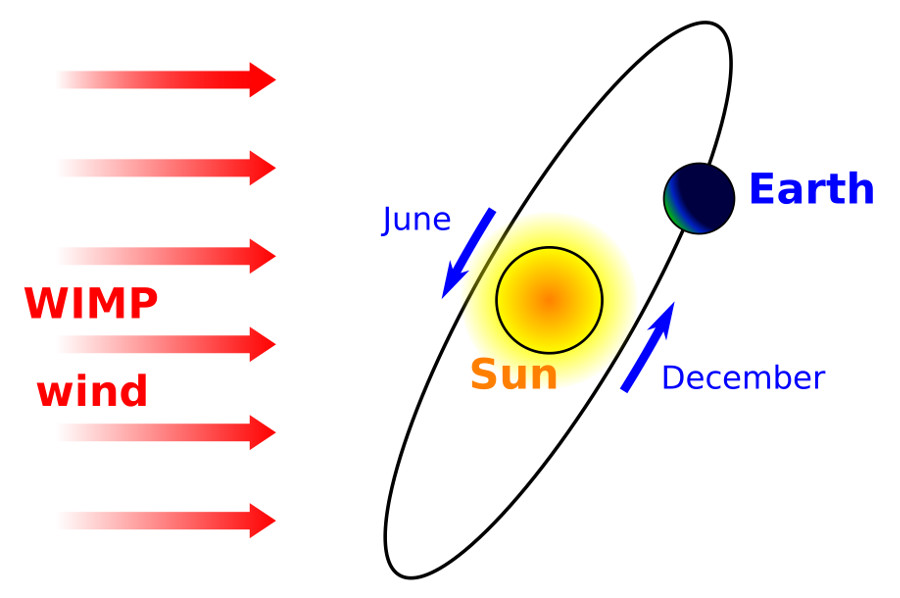
\includegraphics[width=0.6\textwidth]{wimp_wind}
\caption{Orientation of the Earth's rotation around the Sun.  The change in alignment of the Earth's and Sun's velocities causes the
amount of dark matter passing through the Earth to change, appearing as a ``WIMP wind'' with a 1-year period.  The annual modulation
should be present for any DM velocity distribution as long as it does not align with that of the Sun.}
\label{fig:direct_detect_modulation}
\end{figure}
 
  
 
 %========
\subsection{Superheated Liquid Detectors}
\label{subsec:bubbles}
Superheated liquid detectors are the most sensitive to WIMP masses in the tens of $\mathrm{GeV/c^2}$ range.  Their limits for
spin-independent
WIMPs are not as stringent as dual-phase noble gas detectors (\secref{subsec:noble_gas}), but for a number of years they have
consistently provided the
strongest constraints in the spin-dependent sector \citeref{PICO2017}.  Their strong sensitivity comes from using fluorinated
halocarbons, as $^{19}$F is the only stable isotope and its unpaired proton
almost always carries 1/2 spin \citeref{Ellis1991, PICASSO2012}.

At ambient temperatures and pressures fluorinated halocarbons are in a metastable state.  A colliding particle will transfer some of its
heat, which can result in nucleation that is observed acoustically or optically.  By varying the temperature and pressure settings
superheated detectors can reduce $\gamma$ and $\beta$ interactions by a factor of 10$^{9}$, making them a great candidate for a
spin-dependent dark matter discovery.

Superheated detector collaborations include Project In CAnada to Search for Supersymmetric Objects (PICASSO) \citeref{PICASSO2017},
Chicagoland Observatory for Underground Particle Physics (COUPP) \citeref{COUPP2012},
PICO (merged from PICASSO and COUPP) \citeref{PICO2017}, Superheated Instrument for Massive ParticLe Experiments (SIMPLE)
\citeref{SIMPLE2012}, and Materia OSCura A Bolle (MOSCAB) \citeref{MOSCAB2017}.  \figref{fig:sd_limits} shows the exclusion plot of
spin-dependent WIMP-proton cross sections.


\begin{figure}
 \centering
 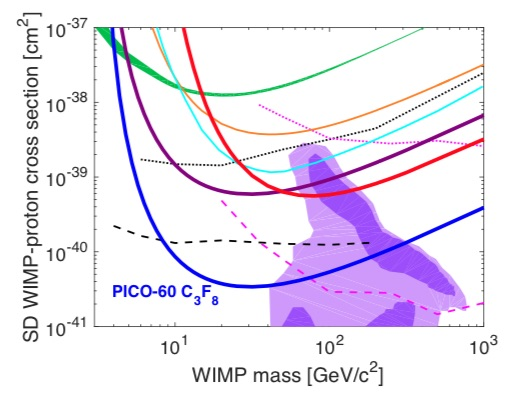
\includegraphics[width=0.8\textwidth]{spin_dependent_limits}
 \caption{Spin-dependent WIMP-proton cross-section 90\% C.L. limits for PICO-60 C$_{3}$F${8}$ (thick blue), PICO-60 CF$_{3}$I (thick red,
 \citeref{PICO2016a}), PICO-2L (thick purple, \citeref{PICO2016b}), PICASSO (green, \citeref{PICASSO2017}), SIMPLE (orange,
 \citeref{SIMPLE2014}), PandaX-II (cyan, \citeref{PandaXII2016a}), IceCube (dashed and dotted pink, \citeref{IceCube2017}), and SuperK
 (dashed and
 dotted black, \citeref{SuperK2011, SuperK2015}).  The shaded purple region is constrained parameter space for the minimal
 supersymmetric model from \citeref{Roszkowski2007}.
 Image credit: \citeref{PICO2017}.}
 \label{fig:sd_limits}
\end{figure}

%When superheated liquid detectors were first considered for WIMP detectors there were some crucial points
%that needed to be addressed.  The downtime of such a detector was high because the temperature
%For WIMP searches modifications had to be made from the original
%devices including increased stability for near-continuous operation and operation as a counting experiment
%\citeref{Pullia2014}.

 %========
\subsection{Scintillation Crystals}
\label{subsec:crystals}
Another target for DM searches is highly radiopure scintillating crystals.  Typically sodium iodide (NaI) or cesium iodide (CsI) is
chosen, with NaI being the most common.  Their sensitivity to SI
and SD DM, low energy threshold, room temperature operability, and ability to run over long periods of time
make them an attractive option.  Doping with thallium increases their light emission and shifts their wavelengths, making the crystals
more transparent and improving phototube detection efficiency \citeref{Undagoitia2016}.  However, trace amounts of radioactive elements
are present in NaI(Tl) crystals \citeref{DAMALIBRA2008}.  The 3 keV x-ray/Auger electron from the decay of
$^{40}$K to \ce{^{40}Ar} through electron capture is particularly concerning because it lays in the region of interest.  In addition a
flat background is produced by $^{238}$U, $^{232}$Th,
and $^{87}$R.  Additionally, the features of the scintillation
does not change for different types of interactions (e.g. $\gamma$-ray, neutron), so particle discrimination is not possible, with the
excepting of rejecting events with multiple scatters.  Thus differentiating between background from signal on an event by event basis is
not possible.  This has made improved radiopurity an increasingly important goal \citeref{Shields2015}.

\begin{figure}
\centering
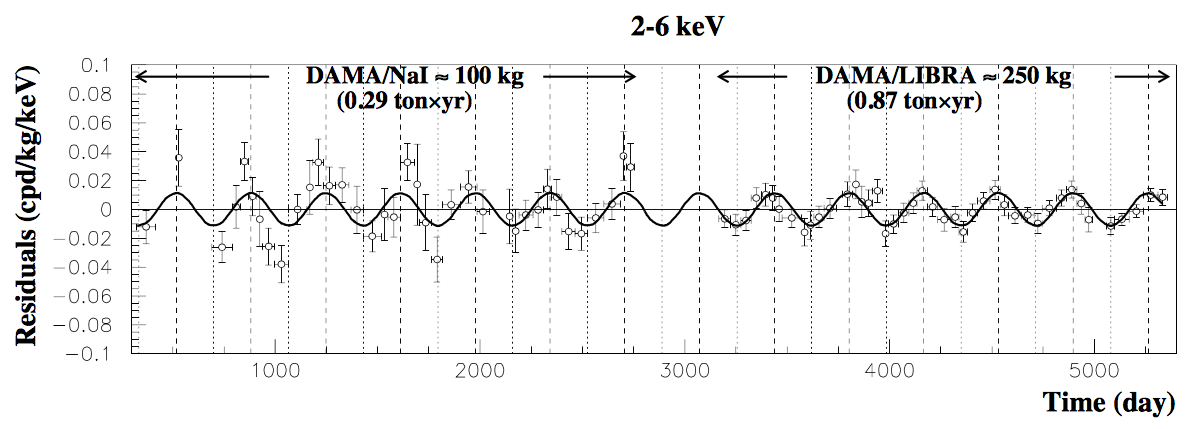
\includegraphics[width=\textwidth]{DAMAModulation}
\caption{Residual event rate between 2-6 \kevee as measured by DAMA/NaI and DAMA/LIBRA.  A fit of $A \cos [\omega (t - t_{0})]$ where
$t_{0} = \mathrm{June\ 2nd}$ and $A$ is the best-fit amplitude is overlaid, with verticale dashed lines corresponding to expected
maxima.  For 14 years they have observed an annual
modulation with $9.3\sigma$.  Claiming this modulation is due to dark matter is controversial, as they are unable to
discriminate between different interaction types and a number of experiments have surpassed their sensitivity with no significant
findings.  Image credit: \citeref{Bernabei2013}.}
\label{fig:dama}
\end{figure}

The DAMA/NaI and its successor DAMA/LIBRA experiments are located underground at the Laboratori Nazionali del Gran Sasso (LNGS) in
L'Aquila, Italy.  They use NaI(Tl) crystals, which allows them to be sensitive to both low- (Na) and high-mass WIMPs from Na and I,
respectively \citeref{DAMALIBRA2008}.  For over 14 annual cycles they have observed an annual modulation in the
2-6 \kevee (\secref{subsubsec:tpcs_signals_energy})
range with 9.3$\sigma$ \citeref{DAMA2013}.  This corresponds to WIMP masses of $10 \mdash 15\ \mathrm{GeV/c^2}$ for sodium-scatters
and 60-100 GeV for iodine.  Their results are shown in \figref{fig:dama}.  Because NaI(Tl) cannot distinguish scatterings of different
particles there is doubt on whether their signal
is caused by WIMPs, or even dark matter.  Spin-independent, spin-dependent or mixed coupling \citeref{Bernabei2001}
and inelastic scattering \citeref{Bernabei2002} WIMPs 
have been considered.  Furthermore, since they cannot specify if the interactions are with nuclei or electrons, alternative dark matter
electron-coupling models \citeref{Bernabei2006} have been examined.  Their results are controversial because other experiments
have surpassed the DAMA/LIBRA sensitivity and see no signal \citeref{Aprile2017a}.  This has prompted theories to explain the annual
modulation via
Standard Model particles.  Hypotheses include known variation in muon flux due to changing stratosphere temperatures, which exhibits
annual modulation in a phase similar to DAMA/LIBRA's findings \citeref{Blum2011}, an incomplete understanding of neutron backgrounds
\citeref{Ralston2010}, or using a combination of muon-induced neutrons and soloar neutrinos \citeref{2014Davis} (this
has been received pushback in \citeref{Barbea2014, Klinger2015}).  The Sodium Iodide with Active Background REjection (SABRE) experiment
is being constructed at LNGS and plans on beginning to take data by the end of 2018 \citeref{Shields2015, SABRE2018}.  By using the same
technology and location they will be the first experiment to directly challenge DAMA/LIBRA.

 %========
\subsection{Germanium Detectors}
\label{subsec:germanium}
High purity germanium (HPGe) detectors measure ionization and offer exceptional energy resolution.  Like scintillation crystals,
(\secref{subsec:crystals}) they can reach very low energies (${\sim} 0.5\ \mathrm{keV}$), making them a promising candidate for low-mass
WIMP (${\sim} 10\ \mathrm{GeV/c^2}$) detection.  It is not possible to differentiate between nuclear recoils from electronic, but
p-type doped detectors have a dead layer on the surface and can use the
pulse rise time to reject background surface events.  In 2010 the Coherent Germanium Neutrino Technology (CoGeNT) experiment
announced it observed an annual modulation similar to DAMA/LIBRA \citeref{CoGeNT2010}.  After continued observation they found the
modulation had a best-fit
WIMP mass of $m_{\chi}\sim 8\ \mathrm{GeV/c^2}$ at a $2.2\sigma$ \citeref{CoGeNT2014}.  However, subsequent analyses with
different
background assumptions showed this significance fell well below 1.7$\sigma$ \citeref{Aalseth2014, Davis2014}.  The China Dark Matter
EXperiment (CdEX) uses the same setup as CoGeNT and found contradictory results \citeref{CDEX2014}, as did CDMS II for nuclear recoils
only \citeref{CDMS2012}.


%========
\subsection{Cryogenic Bolometers}
\label{subsec:bolometers}
Cryogenic bolometers are typically cooled to $10 \mdash 100$ mK so they can detect phonons, allowing a low energy threshold and
outstanding energy resolution.  The Cryogenic Dark Matter Search (CDMS) collaboration uses silicon and germanium detectors where they
measure both phonons
and ionization.  The ionization-to-phonon ratio is used for discrimination where less than 1 in $10^{6}$ of all electronic recoil events
are rejected in the $10 \mdash 100$ keV range \citeref{CDMS2015}.  In 2013 an excess of events was reported with a best-fit
WIMP mass of $8.6\ \mathrm{GeV/c^2}$ \citeref{Agnese2013}.  However, subsequent measurements did not observe such an excess, nor did
EDELWEISS (Exp\'erience pour DEtecter Les WIMPS En Site Souterrain), which has an analogous setup \citeref{EDELWEISS2016}.

The CRESST-II (Cryogenic Rare Event Search with Superconducting Thermometers) experiment measured phonons as well as scintillation using
CaWO$_{4}$ crystals.  They also observed excesses of
events at WIMP masses of 11.6 $\mathrm{GeV/c^2}$ at 4.2$\sigma$ and 25.3 $\mathrm{GeV/c^2}$ at 4.7$\sigma$ \citeref{CRESST2012}, but after
an upgrade reduced their background they were ruled out \citeref{CRESST2015}.


 %========
\subsection{Liquid Noble Gas Detectors} \label{subsec:noble_gas}
Liquid noble gas detectors have led the field for spin-independent WIMP masses at $\gtrsim 20\ \mathrm{GeV/c^2}$, as seen in
\figref{fig:si_limits}.  Commissioned detectors have
used either liquid argon (LAr) or liquid xenon (LXe) and the DEAP/CLEAN
(Dark Matter Experiment using Argon Pulse-Shape/Cryogenic Low-Energy Astrophysics with Noble Liquids ) collaboration is constructing a
detector than can house
LAr and liquid neon (LNe) independently \citeref{Kearns2012, CLEAN2015}.  Advantages of liquid noble gas detectors
include scaleability, particle discrimination, and self-shielding, among others.  As the target mass of these detectors passes
the 1-ton mark they are becoming sensitive to neutrinos, which introduces a new background but can also offer another branch of physics to
study.  Predicted integral rates for xenon, argon, and neon, as well as germanium are shown in \figref{fig:material_wimp_rate}.

\begin{figure}
\centering
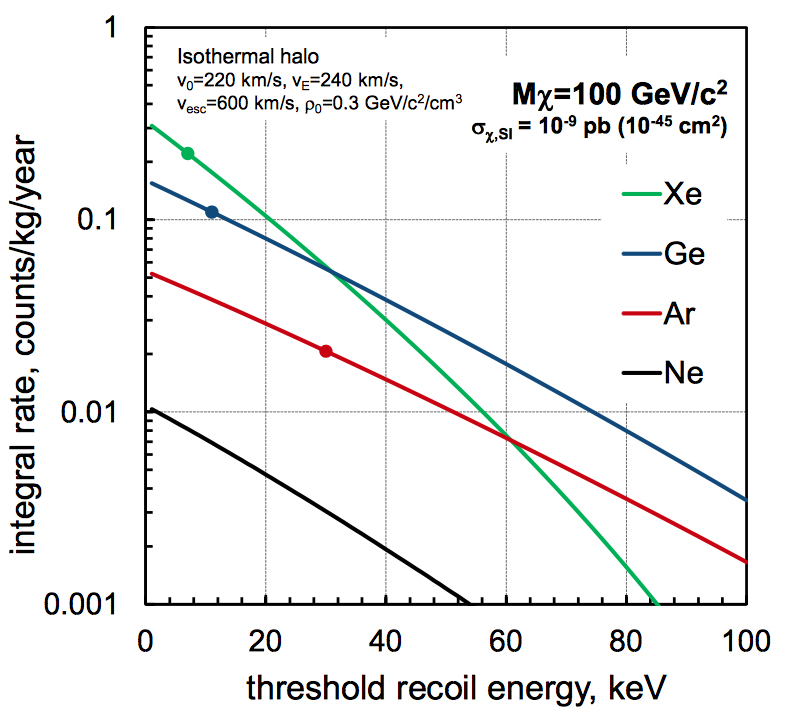
\includegraphics[width=0.6\textwidth]{IntegralRateTargets}
\caption{Expected integral spectra for Xe, Ge, Ar, and Ne for spin-independent elastic scattering of a $100\ \mathrm{GeV/c^2}$ WIMP with
cross section $\sigma = 10^{-45}\ \mathrm{cm^{2}}$ per nucleon.  The rates assume perfect energy resolution and are calculated using the
Standard Halo Model.  The dots correspond to average thresholds for each element.  Image credit: \citeref{Cushman2013}.}
\label{fig:material_wimp_rate}
\end{figure}

Liquid noble gas detectors can be single- or dual-phase.  Dual phase use an electric field to drift electrons to the liquid surface, where
they are extracted across a gas gap and generate a second scintillation.  Single-phase detectors measure only the scintillation and are
typically
spherical.  Because they do not drift electrons they benefit from 4$\pi$ photo-detection (in dual phase this would interfere with the
electric field).  Dual phase experiments are discussed in detail in \chapref{chap:liquid_xe}.  \figref{fig:si_limits} shows the
current status of spin-independent limits.

\begin{figure}
\centering
\includegraphics[width=\textwidth]{si_limits}
\caption{Status of spin-independent WIMP cross section from $0.5 \mdash 1000\ \mathrm{GeV/c^2}$ before XENON1T run-combined analysis
(\chapref{chap:xenon1t}).  Regions of possible signals from DAMA/LIBRA (shaded green, \citeref{DAMA2009}) and the silicon
detector of CDMS II (shaded blue, \citeref{CDMS2013}) are shown.  Exclusion limits from PICO-60 (solid yellow, \citeref{PICO2017}),
DEAP-3600 (dashed purple $> 20\ \mathrm{GeV/c^2}$,
\citeref{DEAP2017}), SuperCDMS (dashed blue, \citeref{SuperCDMS2017}), NEWS-G (dashed purple $< 20\ \mathrm{GeV/c^2}$,
\citeref{NEWSG2018}), CRESST (solid red, \citeref{CRESST2016}), CDMSLite2 (solid blue, \citeref{CDMSLite2016}), LUX
(solid orange, \citeref{LUX2017a}), PandaX-II (solid dark blue 2016
\citeref{PandaXII2016a}, dashed dark blue, 2017 \citeref{PandaXII2017}), XENON100 (solid green, \citeref{Aprile2012c}), and
XENON1T First Results (dashed green, \citeref{Aprile2017f}) are plotted.  Four typical super-symmetric (SUSY) models (CMSSM, NUHM1, NUHM2,
and pMSSM10) with constraints from ATLAS Run
1 are shown for reference \citeref{Bagnaschi2015}.  The cross section of neutrino coherent scattering is marked by the orange dashed
line and shaded region.  Image credit: \citeref{Patrignani2016}.}
\label{fig:si_limits}
\end{figure}


% read https://www.hindawi.com/journals/ahep/2014/387493/ to rewrite above section
%%This is the second chapter of the dissertation

%The following command starts your chapter. If you want different titles used in your ToC and at the top of the page throughout the chapter, you can specify those values here. Since Columbia doesn't want extra information in the headers and footers, the "Top of Page Title" value won't actually appear.

\pagestyle{cu}
\graphicspath{{./Chapter2/Figures/}}
\chapter[Liquid Xenon and Time Projection Chambers][Liquid Xenon and Time Projection Chambers]{Liquid Xenon and Time Projection Chambers}
\label{chap:liquid_xe}

Liquid xenon (LXe) direct detection experiments have led the field for spin-independent WIMP searches with masses $\gtrsim 20$ for roughly
a decade.  More so than liquid argon (LAr), LXe results have been paved the way to new limits, surpassing on the way only those of
other
LXe experiments.

Commercial business, such as steelmaking and coal gasification, rely relatively pure oxygen or nitrogen.  During the separation,
the small amount of xenon and krypton in the air is extracted into a mixture as a by-product.  A distillation process can uncouple
the two, leaving highly pure xenon.

This chapter begins by discussing general properties of xenon and why it is such an effective element for a dark matter search
(\secref{sec:properties}) followed by a summary of signal production (\secref{sec:scintillation}) and then determining the type of
interaction based on its signal properties (\secref{sec:interactions}).

%====================================
\section{General Properties}
\label{sec:properties}
Xenon is a noble gas with atomic number 54 with and a mean molar mass of 131.293 g mol$^{-1}$.  It is the heaviest non-radioactive noble
gas and due to its full valence electron
shell rarely undergoes chemical reactions.  It has a concentration of 87 parts per billion (ppb)
in the Earth's atmosphere at a density of
5.894 g l$^{-1}$.  The phase diagram for xenon is shown in \figref{fig:phase_diagram} and \tabref{tab:xe_properties} lists general
chemical properties.

\begin{figure}
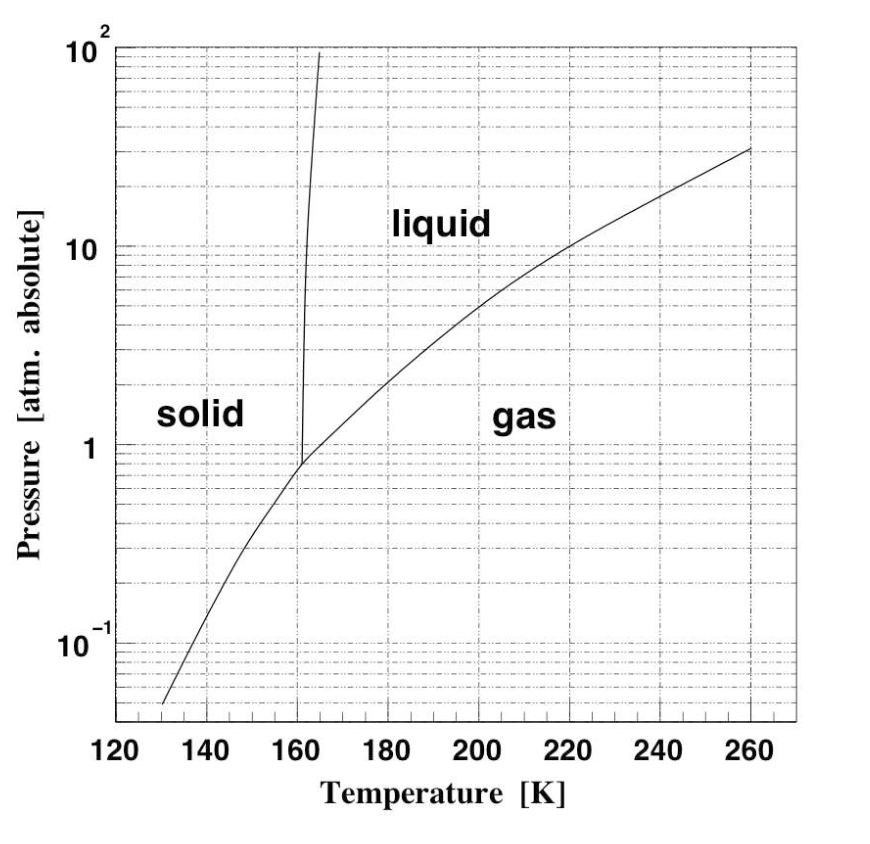
\includegraphics[width=0.6\textwidth]{PhaseDiagram}
\caption{Phase diagram of xenon.  Image credit: \citeref{Aprile2009}.}
\label{fig:phase_diagram}
\end{figure}
 
\begin{table}[t]
 \centering
 \begin{tabular}{cc}
 \hline
 \hline
 Chemical Property & Value \\
 \hline
 Atomic Number & 54 \\
 Molar mass & 131.293 g mol$^{-1}$ \\
 Melting point (1 atm) & 161.4 K \\
 Boiling point (1 atm) & 165.0 K \\
 Density as gas (298 K, 1 atm)  &  5.40 g l$^{-1}$ \\
 Density as gas (165 K, 1 atm)  &  9.99 g l$^{-1}$ \\
 Density as liquid (165 K, 1 atm) & 2.94 g cm$^{-3}$ \\
 Critical point & $16.59^{\circ}$C, 57.65 atm, 1.155 g cm$^{-3}$ \\
 Dielectric constant & 1.95 \\
 Triple point & $-111.74^{\circ}$C, 0.805 atm, 3.08 g cm$^{-3}$ \\
 Thermal conductivity & $5.65 \times 10^{-3}\ \mathrm{W\ m^{-1}\ K^{-1}}$ \\
 Covalent radius & $140 \pm 9$ pm \\
 \hline
 \hline
 \end{tabular}
 \caption{Chemical properties for xenon.  Data taken from \citeref{Baudis2014}.}
\label{tab:xe_properties}
\end{table}

The naturally occurring xenon isotopes are listed in \tabref{tab:xe_isotopes}.  \ce{^{136}Xe}, which makes up 8.8573\% of natural xenon,
has been measured to undergo double beta decay with a half-life of $t_{1/2} > 2.4 \times 10^{21}\ \mathrm{y}$.  \ce{^{124}Xe},
\ce{^{126}Xe},
and \ce{^{134}Xe} are also predicted to to be unstable but decays have not been observed so they are not considered when building a
liquid xenon detector or analyzing data \citeref{Barros2014}.

Unstable isotopes with $t_{1/2} > 1\ \mathrm{h}$ are given in \tabref{tab:xe_unstable_isotopes}.  The longest-lived isotope is
\ce{^{127}Xe} with $t_{1/2} = 36.4\ \mathrm{d}$.  Also listed are metastable states $\mathrm{^{129m}Xe}$, $\mathrm{^{131m}Xe}$, and
$\mathrm{^{133m}Xe}$ with energies 163.9, 236.2, and 233.2 keV $\gamma$-rays, respectively.  $\mathrm{^{129m}Xe}$ and $\mathrm{^{131m}Xe}$
are more commonly produced since \ce{^{129}Xe} and \ce{^{131}Xe} are stable and make up $> 47\%$ of natural xenon
(\tabref{tab:xe_isotopes}).  Following a nuclear recoil calibration they are used to measure a number of properties about our detector
including the electron lifetime (\secref{subsec:electron_lifetimes_measurement_gammas}).  Their shorter-lived 39.6
(\ce{^{129}Xe}) and 80.2 (\ce{^{131}Xe}) keV nuclear
excited states, which have $t_{1/2} = 0.97\ \mathrm{ns}$ and 0.48 ns, respectively, are rarely resolvable from the signal of the
particle-nucleus scatter.

Xenon has several advantages that make it a good target for dark matter detection.  At \$2000/kg it is scaleable for larger
detectors.  Its high molar mass provides excellent self-shielding, which reduces background contamination in the region of interest due to
external radiation
(\secref{subsec:backgrounds_detector_materials}).  Furthermore, nearly 50\% of naturally occurring xenon is $^{129}$Xe or $^{131}$Xe,
which gives it sensitivity to spin-dependent interactions.  Its production of light and charge - referred to as light and charge yields
(\secref{subsubsec:er_nr_calibrations_results_ly_qy}) - are among the highest noble gases.  Finally, the expected background contribution
from xenon itself comes just from \ce{^{136}Xe} so is extremely small (\tabref{tab:xe_isotopes}).  Therefore
intrinsic radioactivity comes almost entirely from trace amounts of other radioactive noble gases, which can be reduced
(\secref{subsec:xenon1t_kr_dist}).


\begin{table}
 \centering
 \begin{tabular}{ccccc}
 \hline
 \hline
 Isotope & Natural Abundance [\%] & Spin & Half-life & Decay mode \\
 \hline
 $^{124}$Xe & 0.0952 & 0 &  $> 1.6 \times 10^{14}\ \mathrm{y}$ & $2\nu \beta^{+} \beta^{+}$ \\
 $^{126}$Xe & 0.089 & 0 & $> 4.7 \mdash 12 \times 10^{25}\ \mathrm{y}$ & $2\nu \beta^{+} \beta^{+}$ \\
 $^{128}$Xe & 1.910 & 0 & stable & $-$ \\
 $^{129}$Xe & 26.401 & 1/2 & stable & $-$ \\
 $^{130}$Xe & 4.071 & 0 & stable & $-$ \\
 $^{131}$Xe & 21.23 & 3/2 & stable & $-$ \\
 $^{132}$Xe & 26.909 & 0 & stable & $-$ \\
 $^{134}$Xe & 10.436 & 0 &  $> 5.8 \times 10^{22}\ \mathrm{y}$ & $2\nu \beta^{-} \beta^{-}$ \\
 $^{136}$Xe & 8.857 & 0 &  $> 2.4 \times 10^{21}\ \mathrm{y}$ & $2\nu \beta^{-} \beta^{-}$ \\
 \hline
 \hline
 \end{tabular}
 \caption{Properties of naturally occurring xenon isotopes.  Decays of \ce{^{124}Xe}, \ce{^{126}Xe}, and \ce{^{134}Xe} have not been
 observed but are predicted.  \ce{^{124}Xe} is predicted to also decay by $2 \nu \beta^+ \mathrm{EC}$ and
 $2 \nu \mathrm{ECEC}$.  Half-life and decay information is taken from \citeref{Singh2007, Barros2014}.}
\label{tab:xe_isotopes}
\end{table}

\begin{table}
\centering
\begin{tabular}{ccccc}
\hline
\hline
Isotope & Spin & Half-life & Decay mode & Decay product \\
\hline
$^{122}$Xe & 0 & 20.1 h & EC & \ce{^{122}I} \\
$^{123}$Xe & 1/2 & 2.08 h & EC & \ce{^{123}I} \\
\ce{^{125}Xe} & 1/2 & 17.1 h & EC & \ce{^{125}I} \\
\ce{^{127}Xe} & 1/2 & 36.4 d & EC & \ce{^{127}I} \\
$\mathrm{^{129m}Xe}$ & 11/2 & 8.88 d & $\gamma$-ray & ground state \\
$\mathrm{^{131m}Xe}$ & 11/2 & 11.93 d & $\gamma$-ray & ground state \\
\ce{^{133}Xe} & 3/2 & 5.24 d & $\beta^-$ & \ce{^{133}Cs} \\
$\mathrm{^{133m}Xe}$ & 11/2 & 2.19 d & $\gamma$-ray & ground state \\
\ce{^{135}Xe} & 3/2 & 9.14 h & $\beta^-$ & \ce{^{135}Cs} \\
\hline
\hline
\end{tabular}
\caption{Unstable isotopes of xenon with half-lifes of $> 1\ \mathrm{hr}$.  Spins, half-lifes, decay modes, and decay products are
listed.}
\label{tab:xe_unstable_isotopes}
\end{table}

\begin{figure}
\centering
\includegraphics[width=0.8\textwidth]{Figure 1 from SeeFig15}
\end{figure}



%====================================
\section{Signal Production}
\label{sec:scintillation}
As radiation scatters off a xenon atom it will cause photon emission due to two effects.  The first is electrons excited to
higher orbitals will quickly de-excite, with the energy carried away by photons.  The second possibility is ionized xenon may
recombine with an
electron (can but doesn't need to be its own), after which it is in an excited state equivalent to the first scenario.  In the
context of this and other experiments the photons are observed as primary (or prompt) scintillation.  Secondary scintillation results from
electrons that do not recombine and is measured only in a time-projection
chamber (TPC).  This chapter only considers interactions in xenon in the presence of an electric field, unless otherwise
specified.



%========
\subsection{Primary Scintillation}
\label{subsec:primary}
When a particle scatters off a xenon atom it can excite or ionize its valence electrons.  A freed electron can escape or recombine with a
Xe$^{+}$.  Excitons Xe$^{*}$ can bond with another Xe atom to create
dimers, Xe$_{2}^{*}$, commonly referred to as excimers.  The processes of recombination is shown in \eqnref{eq:recomb}, where $Q$
represents heat.

If the interaction occurs in an electric field some $e^{-}$ will be pulled from the site, which lowers recombination and therefore
decreases primary
scintillation and increases secondary scintillation (\secref{subsec:secondary}).  The extent to which recombination changes depends on the
strength of the electric
field.  However, even without a field there will not be
100\% recombination because some of the freed $e^{-}$ will escape the electromagnetic pull of their parent ions.

\begin{subequations}
\begin{align}
\mathrm{Xe}^{+} + \mathrm{Xe} &\rightarrow \mathrm{Xe}_{2}^{+} \\
\mathrm{Xe}_{2}^{+} + e^{-} &\rightarrow \mathrm{Xe}^{**} + \mathrm{Xe} \\
\mathrm{Xe}^{**} &\rightarrow \mathrm{Xe}^{*} + Q
\end{align}
\label{eq:recomb}
\end{subequations}

The Xe$^{*}$ that has results from recombination is equivalent to if it had only ever been excited.  At this point
it de-excites via \eqnref{eq:deexcite}.  Xe$_{2}^{*}$ is in either a singlet
($^{1}\Sigma$) or triplet ($^{3}\Sigma$) state and quickly de-excites to the ground state.

\begin{subequations}
\begin{align}
\mathrm{Xe}^{*} + \mathrm{Xe} &\rightarrow \mathrm{Xe}_{2}^{*} \\
\mathrm{Xe}_{2}^{*} &\rightarrow 2\mathrm{Xe} + \gamma
\label{eq:deexcite_gamma}
\end{align}
\label{eq:deexcite}
\end{subequations}

The average \gammaray in \eqnref{eq:deexcite_gamma} has a wavelength of 178 nm.  Not surprisingly, the number of photons is
anti-correlated with the number of electrons, since for each \electron that
recombines with xenon a \gammaray is emitted.  The lifetimes for the singlet and triplet
excimers are $3.1 \pm 0.7$ ns and $24 \pm 1$ ns, respectively \citeref{Mock2014}.  The singlet-to-triplet ratios for
a number of different interactions are shown in \tabref{tab:singlet_to_triplet}.  Detecting WIMPS requires differentiating between
scatters with the xenon electron shells (electronic recoils) and nucleus (nuclear recoils).  \tabref{tab:singlet_to_triplet} shows that
nuclear recoils result in a higher fraction of singlet states.  Unfortunately the $^1\Sigma$ and $^3\Sigma$ lifetimes
are too short to resolve so they cannot be used for discrimination.  This makes single-phase LXe detectors
less desirable than liquid argon (LAr), which has single and triplet states of $< 6.2$ ns and $1.30 \pm 0.06\ \mathrm{\mu s}$
\citeref{Heindl2011}.

\begin{table}[t]
 \centering
 \begin{tabular}{cc}
 \hline
 \hline
 Event & $^1\Sigma / ^3\Sigma$ \\
 \hline
 ER (direct excitation from $\gamma$) & $0.17 \pm 0.05$ \\
 ER (recombination from $\gamma$) & $0.8 \pm 0.2$ \\
 ER (from $\alpha$) & $2.3 \pm 0.51$ \\
 NR (from neutron) & $7.8 \pm 1.5$ \\
 \hline
 \hline
 \end{tabular}
 \caption{Error-weighted average of world data for single-to-triplet ratios for various scattering cases \citeref{Mock2014}.}
\label{tab:singlet_to_triplet}
\end{table}

\figref{fig:interaction_channels} shows the interaction
channels of $\beta$- or $\gamma$-induced xenon recoils described in \eqnref{eq:recomb} and \eqnref{eq:deexcite}.
However, in nuclear recoils
it has been observed that two excitons may collide and free an electron as shown in \eqnref{eq:biexcitonic} in what is known as
biexcitonic quenching (\secref{subsec:recombination}).

\begin{figure}
\centering
\includegraphics[width=0.8\textwidth]{interaction_channels}
\caption{Signal generation pathways for electronic and nuclear recoils.  Describe paths of electrons.  Image credit: \citeref{Faham2014}.}
\label{fig:interaction_channels}
\end{figure}




%========
\subsection{Secondary Scintillation}
\label{subsec:secondary}
In an electric field $E$ an \electron that is freed but does not recombine with its parent or other ions will move anti-parallel
to the field at drift velocity $v_{d}$.  At fields of $\lesssim 100\ \mathrm{V\ cm^{-1}}$ the drift velocity is nearly proportional to
$E$ and is given by $v_{d} = \mu E$
where $\mu$ is the electron mobility, estimated to be ${\sim}2200\ \mathrm{cm^{2}\ V^{-2}\ s^{-1}}$ at these fields
\citeref{Miller1968}.  As
$E$ increases $v_{d} \propto E^{1/2}$ until approximately $10^4\ \mathrm{V\ cm^{-1}}$ where it flattens at
${\sim} 3\ \mathrm{mm\ \mu s}$.  \figref{fig:drift_velocity} shows \vd
as a function of $E$ and \tabref{tab:drift_velocity} gives the approximate relationship.

In liquid noble gas detectors used for dark matter searches electrons are drifted to the surface of the liquid and
extracted across ${\sim}5\ \mathrm{mm}$ of xenon gas.  As the electrons drift across the gas they excite and ionize new xenon atoms,
creating a second signal referred to as secondary scintillation.  Because the amount of scintillation
produced per electron is independent of the number of electrons extracted this is also known as proportional scintillation.  By
measuring this scintillation the number of \electron extracted can be determined.  Details of \electron drift and proportional
scintillation is found in \secref{subsec:tpcs_working_principle}.

\begin{table}
 \centering
 \begin{tabular}{cc}
 \hline
 \hline
 $E$ [V cm$^{-1}$] & $E$ dependence \\
 \hline
 $\lesssim 100$ & $E$ \\
 ${\sim} 100 \mdash 10^{3 \mdash 4}$ & $E^{1/2}$ \\
 $\gtrsim 10^{4}$ & $-$ \\
 \hline
 \hline
 \caption{Drift velocity \vd as a function of electric field $E$ for LXe}
 \end{tabular}
 \label{tab:drift_velocity}
\end{table}

\begin{figure}
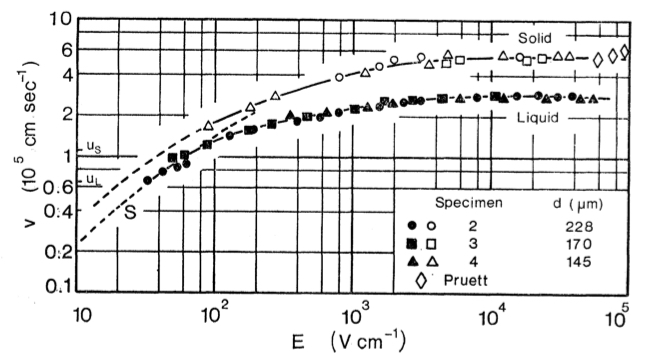
\includegraphics[angle=0.5, width=0.8\textwidth]{DriftVelocity}
\caption{Field-dependent drift velocity for solid ($-116^{\circ}\mathrm{C}$) and liquid ($-110^{\circ}\mathrm{C}$) xenon.  Image credit:
\citeref{Miller1968}.}
\label{fig:drift_velocity}
\end{figure}




%====================================
\subsection{Stopping Power}
\label{subsec:stopping_power}
A particle that loses energy through inelastic collisions with electrons (prompting excitation and ionization) produces an electronic
recoil.  The energy lost per unit
length is the electronic stopping power $S_{\mathrm{elec}}(E) = -(dE/dx)_{\mathrm{elec}}$ ($S_{\mathrm{elec}}$ is positive).  It is
correlated with the linear energy transfer (LET) and depends on the type and energy of the particle and properties of the
medium (e.g. density and composition).  A larger electronic stopping power indicates the particle will slow more quickly and
transfer its energy more densely along its track.  This affects recombination between \electron and ions and is discussed in
\secref{subsec:recombination}.

\begin{figure}[t]
\includegraphics[width=0.8\textwidth]{stopping_power_components}
\caption{Mass stopping power for alphas (blue), $e^{-}$ (green), and protons (pink).  Electronic (long dashed), nuclear (short dashed),
and total (solid) stopping powers for each are shown.  The electronic stopping power is more significant except for $e^-$ at
$\gtrsim 15\ \mathrm{MeV}$.  Data from \citeref{Berger2018a}.}
\label{fig:mass_stopping_power}
\end{figure}

The energy loss per unit length of a particle through elastic collisions with atoms is the nuclear stopping power
$S_{\mathrm{nucl}}(E) = -(dE/dx)_{\mathrm{nucl}}$.  In contrast to electronic stopping power,
$S_{\mathrm{nucl}}(E)$ quantifies the slowing of the particle due to interactions with nuclei of the target and can be calculated using
the repulsive potential energy between atoms.

Dividing the stopping power by the medium's density ($S(E) / \rho$) gives a function of the incident particle known as
the mass stopping power.  Electronic (long dashed) and nuclear (short) mass stopping powers are shown for alphas, electrons, and protons
in \figref{fig:mass_stopping_power}.  $S_{\mathrm{elec}} > S_{\mathrm{nucl}}$ over all energy except for electrons above roughly 15
MeV.  The total stopping power is

\begin{equation}
\bigg( \frac{dE}{dx} \bigg)_{\mathrm{tot}} = \bigg( \frac{dE}{dx} \bigg)_{\mathrm{elec}} + \bigg( \frac{dE}{dx} \bigg)_{\mathrm{nucl}}
\end{equation}

\noindent and is shown as the solid lines in \figref{fig:mass_stopping_power}.  The mean path length of a particle with initial energy
$E_0$ can be approximated by

\begin{equation}
\Delta x = \int_0^{E_0} \frac{1}{S(E)}\, dE
\label{eq:stopping_power_dist_trav}
\end{equation}

\noindent where $\Delta x$ is the continuous slowing down approximation (CSDA) and
$S(E) \equiv -(dE/dx)_{\mathrm{tot}}$.  \eqnref{eq:stopping_power_dist_trav} does not account for energy-loss
fluctuations.  For spin-independent
WIMP dark matter searches the relevant energy range for electrons is $1 \mdash 20$ keV.  In this region $S(E)/\rho$ decreases so
electrons with more energy will travel farther by a ratio greater than their energy.  Alphas do not affect
our dark matter search since they are in the MeV range and are easily identified by their large primary scintillation.  The
\alphadecays that are relevant in our detector sit mostly around 5-7 MeV so have a stopping power between
$200 \mdash 400\ \mathrm{MeV\ cm^2\ g^{-1}}$.  In this region their mass stopping power also decreases with energy.  The $\alpha$ and
proton curves have similar shapes because they are both described by the Bethe formula \citeref{Bethe1937}.

One of the biggest advantages of liquid xenon is its large stopping power (largely due to its high atomic
mass), which provides self-shielding.  Because distance and stopping power are anti-correlated, particles in LXe travel relatively short
distances before stopping.  Self-shielding protects the interior of the detector from outside radiation,
which rarely penetrates more than a few cm
into the LXe, allowing a larger fiducial volume (FV) for dark matter searches.  Because the stopping power is proportional to the
density of the medium, LXe is more effective at self-shielding than liquid argon ($\rho = 1.395\ \mathrm{g\ cm^{-3}}$) and liquid neon
($1.207\ \mathrm{g\ cm^{-3}}$).

\begin{figure}
\centering
\includegraphics[width=\textwidth]{recoil_diagram}
\caption{Electronic (top, $\gamma$) and nuclear (bottom, neutron) recoil tracks for 20 keV scatters.  Excitons (red circles), ions
(blue), and
heat (grey) are marked along the track.  The electronic recoil produces ${\sim} 20 \times$ as many ions as excitons while for nuclear
recoil they are roughly equal.  Heat is only relevant in NRs and leads to signal quenching.  The electronic recoil has a path of
${\sim} 1\ \mathrm{\mu m}$ while the much denser 10 nm of the NR compels higher recombination.  Image credit: \citeref{Faham2014}.}
\label{fig:er_nr_recoil_diagram}
\end{figure}

The track structure from a recoiling electron or xenon nucleus is characterized by the distribution of \electron, ions, excitons, and heat
when all electrons have slowed to sub-excitation speeds \citeref{Chepel2013}.  Tracks are typically cylindrical with secondary branches
from $\delta$-ray.  However, aside from this basic structure they can vary considerably with particle, energy, and
stopping power, and they play a major role in recombination.  \figref{fig:er_nr_recoil_diagram} shows tracks for 20 keV electronic and
nuclear
recoils.  For the electronic recoil a \gammaray ionizes the atom and transfers its energy to the freed electron.  As the electron moves
through the xenon it excites and ionizes more atoms, creating secondary branches from $\delta$-rays until it comes to a rest after
roughly $0.5\ \mathrm{\mu m}$.  The number of ions is ${\sim}20$ times as high as the number of excitons.  Because the \electron only
interacts with the electron shells of the atom not energy is lost as heat.

For the nuclear recoil a 20 keV neutron scatters with a xenon nucleus.  Unlike the electronic recoil where the energy of the \gammaray is
passed to the electron (after small loss from ionization) for a nuclear recoil it is passed to the atom.  The higher stopping power
creates a denser track and a shorter average path length of approximately 10 nm.  In addition to exciting and ionizing, the recoiling atom
passes translational energy to other atoms that cannot be observed (\secref{subsec:recombination}).  The exciton-to-ion ratio is roughly
1, and the higher density of ions leads to greater recombination between electrons and non-parent \ce{Xe^+}.


%========
\subsection{Recombination}
\label{subsec:recombination}
A fraction of atoms that are ionized recombine with electrons.  The recombination fraction depends on a number of parameters
including ionization density
(stopping power, \secref{subsec:stopping_power}), thermal energy of ionized atoms and $e^{-}$, electron mobility, diffusion rate, electric
field, and probability of recombination when an electron and ion meet.

An early theory by Onsager modeled recombination by defining what is now known as the Onsager radius as the distance between an
electron-\ce{Xe^+} pair where the Coulomb energy equals the \electron thermal energy \citeref{Onsager1938}.  An electron within the
Onsager radius will be unable to escape so will recombine with the ion.  At the Onsager radius the probability of escape is $e^{-1}$.  An
\electron
with $E_{\mathrm{thermal}} > E_{\mathrm{Coulomb}}$ should not be influenced by the ion, regardless of the presence of an electric
field.  The thermalization range for LXe is $4000 \mdash 5000$ nm \citeref{Mozumder1995}, far higher than the Onsager radius for liquid
xenon of $49$ nm.  Without an electric field a large fraction of these electrons will recombine on
timescales of $> 1\ \mathrm{ms}$, which because of the short observation window will appear as a decrease in photons, and the electrons
will be classified as having escaped (with an electric field the electrons outside the Onsager radius will drift from the interaction site
and not recombine) \citeref{Doke2002}.

A shortcoming of the Onsager radius is that it treats the interactions between Xe$^{+}$ and \electron as strictly Coulomb.  However,
the high coefficient of polarization of LXe produces dipole moments in the ions, causing the electric field to fall faster than
$1/r$.  In fact, the potential is steep enough that the ion travels via phonon-assisted tunneling \citeref{Thomas1987}, making its
mobility significantly smaller (3-5 orders of magnitude \citeref{Miller1968, Yoshino1976}) than that of the electrons.

As a result of these disparities another model was proposed that includes diffusion but the rate of
recombination depends on
the density of \electron and ions independently \citeref{Jaffe1913}.  Its derivation comes by

\begin{subequations}
\begin{align}
\frac{\partial N_{+}}{\partial t} &= -u_{+} \mathbf{E}_d \cdot \nabla N_{+} + d_{+} \nabla^{2} N_{+} - \alpha N_{+} N_{-}
\label{eq:diff_plus} \\
\frac{\partial N_{-}}{\partial t} &= u_{-} \mathbf{E}_d \cdot \nabla N_{-} + d_{-} \nabla^{2} N_{-} - \alpha N_{+} N_{-}
\label{eq:diff_minus}
\end{align}
\label{eq:diff_plus_mins}
\end{subequations}

\noindent where $N_{\pm}$ are the ion ($+$) and electron ($-$) charge distributions ($N_+ = N_-$), $\mu_{\pm}$ are their mobilities,
$d_{\pm}$ and $\alpha$
are the coefficients for diffusion and recombination, and $\mathbf{E}_d$ is the electric field.  The terms on the right sides of
\eqnref{eq:diff_plus} and \eqnref{eq:diff_minus} correspond to the drift, diffusion, and recombination, from left to right.  The
diffusion in xenon is small (millimeters per drift meter \citeref{Deiters1981}) and can be ignored.  Likewise the ion mobility $\mu_{+}$
is several orders of magnitude smaller than that
of the electron and is disregarded.  Thus \eqnref{eq:diff_plus_mins} can be simplified to

\begin{subequations}
\begin{align}
\frac{\partial N_{+}}{\partial t} &= - \alpha N_{+} N_{-}
\label{eq:diff_simple_plus} \\
\frac{\partial N_{-}}{\partial t} &= u_{-} E_d \frac{\partial N_{-}}{\partial z} - \alpha N_{+} N_{-}
\label{eq:diff_simple_minus}
\end{align}
\end{subequations}

\noindent which, if each electron-ion pair is sufficiently far from all others, can be solved exactly.  After some integration and algebra
(detailed in \citeref{Thomas1987}), the recombination fraction is

\begin{equation}
r = 1 - \frac{\mathrm{ln} (1 + N_0 \varsigma)}{N_0 \varsigma},\ \varsigma = \frac{\alpha}{4 a^{2} u_{-} E_d}
\label{eq:ti_recomb}
\end{equation}

\noindent where $N_0$ is the number of ions and electrons at $t = 0$ that uniformly occupies over a box of dimension $a$.  This is known
as the Thomas-Imel box model \citeref{Thomas1987},
and is successful at explaining recombination measurements including those shown in \figref{fig:ti_recomb}.  Zero recombination
corresponds to
$\varsigma \rightarrow 0$ and complete recombination occurs when $\varsigma \rightarrow \infty$.  In this model $E = 0$ equates to total
recombination, though as mentioned above, this likely occurs outside of the typical observation window.

\begin{figure}
\includegraphics[width=0.8\textwidth]{ti_recombination}
\caption{Measurements of charge collected ($q \propto 1 - r$) for LAr and LXe with respect to $E_d$.  Squares correspond to LXe and were
measured with $\varsigma N_0 E = 0.15\ \mathrm{kV\ cm^{-1}}$.  Triangles and circles are LAr and were measured at
$\varsigma N_0 E = 0.84\ \mathrm{kV\ cm^{-1}}$.  Curves are fits to data using the Thomas-Imdel box model \citeref{Thomas1987}.}
\label{fig:ti_recomb}
\end{figure}

The Thomas-Imel box model works well for short particle tracks but has shortcomings for longer.  At long particle tracks a Birks'
Law (originally developed for organic scintillators, \citeref{Birks1951, Birks1964}) derivation for liquid noble gases yields

\begin{equation}
\frac{dN_{\pm}}{dt} = -\alpha N_{+} N_{-}
\label{eq:birks_diff}
\end{equation}

\noindent for volume recombination - that is, for electrons to recombine with a \ce{Xe^+} that is not their parent.  Here $N_{\pm}$ and
$\alpha$ have the same definitions as in the Thomas-Imel model.  \eqnref{eq:birks_diff} is simplified by assuming
$N_{+} = N_{-}$ and the number of each is proportional to the stopping power $N_{\pm} \propto dE/dx$
(\secref{subsec:stopping_power}).  The latter is only valid for
cylindrical, or long tracks.  Short tracks, which correspond to lower LET and therefore $dE/dx$, are described better by a spherical
excitation-ionization density \citeref{Chepel2013}.  This gives a recombination of

\begin{equation}
r = \frac{A \frac{dE}{dx}}{1 + B \frac{dE}{dx}} + C
\label{eq:birks_recomb}
\end{equation}

\noindent where $A$, $B$, and $C$ are constants derived in the fit \citeref{Doke1988}.  The two terms on the right side of the equation
correspond to
non-geminate and geminate recombination, respectively.  Geminate recombination ($C$) quantifies the
\electron that recombine with their parent ions and is governed by Onsager's model with fixed probability for all $dE/dx$
\citeref{NEST2011}.  Non-geminate
(volume) recombination is when an \electron is captured by an ion different than its parent.  This has been shown to be valid at
$E \gtrsim 80\ \mathrm{keV}$ for \gammarays and light ions, and ${\sim} 1\ \mathrm{MeV}$ electrons.

The considerable LET for $\alpha$-particles creates high-density tracks that lead to strong and quick recombination.  The
density is so high only a small percent of \electron avoid recombination, even at electric fields of
${\sim} 10\ \mathrm{kV\ cm^{-1}}$
(for electrons this is nearly 100\%) \citeref{Chepel2013}.  The consistency in charge collection across different fields causes
difficulties in distinguishing recombination from excitation.

Birk's saturation law explains biexcitonic quenching and the Penning process, which play major roles in nuclear recoils.  Biexcitonic
quenching occurs as

\begin{equation}
\mathrm{Xe}^{*} + \mathrm{Xe}^{*} \rightarrow \mathrm{Xe} + \mathrm{Xe}^{+} + e^{-}
\label{eq:biexcitonic_again}
\end{equation}

\noindent where the \electron escapes with kinetic energy $E = 2E_{\mathrm{ex}} - E_{\mathrm{g}}$ where $E_{\mathrm{ex}}$ and
$E_{\mathrm{g}}$ are the energies of an exciton and band gap, respectively.  The \electron will quickly lose its energy and recombine,
resulting in the emission of a single photon instead of two from the initial excitons.  A second quenching comes from collisions between
excimers via the Penning process that results in an excited and ground molecular states \citeref{Mei2008}.  For nuclear recoils these
quenching factors can be parameterized by

\begin{equation}
f_{b} = \frac{1}{1 + k_B B \frac{dE}{dx}}
\label{eq:nr_scint_quench}
\end{equation}

\noindent where $k_B$ is Birks' constant \citeref{Birks1951, Birks1964}.

The decrease in scintillation yield for $\beta$ and $\gamma$ is only observed at low LET where the ionization density is relatively
low.  The
lack of neighboring $\mathrm{Xe}^{+}$ reduces the probability of recombination with a non-parent ion.  At higher LET the ion density
is sufficient for nearly 100\% recombination and results in the flat region in \figref{fig:scintillation_yield}.  However, unlike nuclear
recoils this there is no true decrease in photons and electrons so this effect does not result in quenching.

\begin{figure}
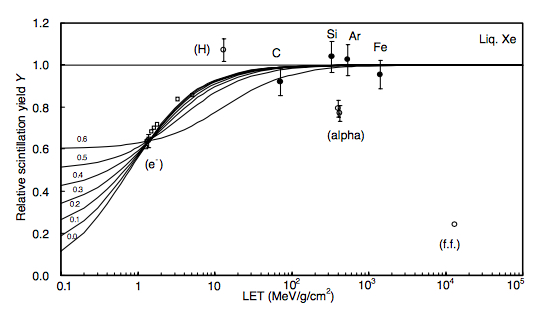
\includegraphics[width=0.8\textwidth]{ScintillationYield}
\caption{Scintillation yield as a function of LET in LXe.  Open circles represent electrons, alpha particles, and fission
fragments.  Solid circles represent relativistic heavy particles.  Open squares mark gamma-rays.  Solid lines trace various fits
to $\beta$-$\gamma$ data from \citeref{Doke2002}.  Image credit: \citeref{Doke2002}.}
\label{fig:scintillation_yield}
\end{figure}



%====================================
\section{Interactions}
\label{sec:interactions}
Because WIMPs are expected to scatter with nuclei electronic recoils are excluded in early analyses (\citeref{Aprile2017f},
\chapref{chap:xenon1t}) as possible signals and considered only as background.\footnote{Results from a WIMP-electron coupling analysis can
be found in \citeref{Aprile2015a}.}  However, understanding the electronic recoil background is necessary to be able to discriminate
against nuclear recoils.  Detector materials have radioactive elements that decay inside the detector, and there are intrinsic
backgrounds such as \krypton and \radon.  The latter is much more concerning since events from
detectors materials cannot breach the inner volume, but intrinsic sources are uniformly distributed throughout the xenon.

To understand our detector calibrations are regularly performed (\secref{subsec:det_char}).  In the ton-scale era of liquid xenon
detectors external sources, which were effective in past experiments, are less efficient because xenon's self-shielding makes it extremely
difficult for radiation to penetrate the interior.  Therefore radioactive
sources that have short half-lifes and can be mixed with the xenon such as $\mathrm{^{83m}Kr}$ and \radoncal are used.  Because these
sources and their progenies have short half-lifes or are stable, they do not contribute to our background after 2-3 days.

\subsection{Photons}
\label{subsec:photons}
Photons produce electronic recoils as they interact with \electron via Compton scattering, pair production, or photoelectric absorption
as shown in \figref{fig:phot_atten}.  Coherent (Rayleigh and Thomson) scattering are also shown though their net energy deposition in the
xenon is zero.

In Compton scattering the photon recoils off of an $e^{-}$ and transfers to it a portion of its energy.  The final energy of the photon
depends only on its initial energy and the scattering angle.  Nuclear Compton scattering is possible but much rarer
\citeref{Christillin1986}.  The low-energy limit of Compton Scattering (photon wavelength larger than particle Compton wavelength) is
Thomson scattering.  Thomson and Rayleigh scattering are elastic so they have a net energy contribution of zero, and are known as coherent
scatters.

Pair production occurs when a high-energy photon produces a particle-antiparticle pair.  Typically this refers to a photon passing
sufficiently
close to an atom's nucleus and creating an electron-positron pair.  The proximity of the nucleus is required to conserve momentum so it
will recoil slightly.  The photon must have an energy of at least twice the electron mass $m_{e}$, or $1.0222\ \mathrm{MeV/c^2}$.  Pair
production
also occurs for a photon in the presence of an atomic electron but is less probable and requires an energy of at least $4m_{e}$.  This
is known as triplet production since the recoiling electron creates a track in addition to the electron-positron pair
\citeref{Hubbell2006}.  At high energies pair production becomes the dominant interaction for photons and matter.

Photoelectric absorption is when an electron absorbs the energy of the photon and is liberated from its electron shell.  In this case the
photon disappears entirely and the kinetic energy of the electron is equal to the photon's energy minus the electron binding
energy.  Photoelectric absorption was helpful for calibrating small detectors using mono-energetic \gammarays from elements such as
\cesium (661.7 keV) and \cobaltsixty
(1.1732 and 1.3325 MeV).  For large detectors self-shielding prevents even high-energy \gammarays from reaching the fiducial
volume, so external sources cannot be used for calibration.  Photoelectric absorption is the dominant interaction in the WIMP search
energy region of interest ($E < 20\ \mathrm{keV}$), and is shown as the red dotted line in \figref{fig:phot_atten}.

\begin{figure}
 \centering
 \includegraphics[width=0.8\textwidth]{photon_scatter}
 \caption{Mass attenuation coefficient and attenuation length for $1\ \mathrm{keV}$ to $100\ \mathrm{MeV}$ photons.  Photoelectric
 absorption (red dashed), Compton scattering (green), coherent (Rayleigh and Thomson) scattering (purple), and pair production (blue) are
 shown in addition to the total (solid black).  The discontinuity at ${\sim}5\ \mathrm{keV}$ occurs just above the binding energy of the
 L-shell electrons and is due to an increase in photoelectric absorption.  A similar process occurs for the K-shell at
 roughly 40 keV.  Data from \citeref{Berger2018b}.}
 \label{fig:phot_atten}
\end{figure}


\subsection[$\beta$-Decays][$\beta$-Decays]{$\mathbf{\beta}$-Decays}
\label{subsec:beta}
\betadecays are the emission of an electron-antineutrino (positron-neutrino) from a neutron (proton).  As with photons, they interact
with the \electron shell and produce electronic recoils.  Because the neutrino carries
some momentum, the energy spectrum of the \electron is not mono-energetic, so it can be difficult to identify the origin of the event.  In
xenon
experiments low-energy \betadecays contribute the most contamination in the search region and occur throughout the entire volume due to
\ce{^{85}Kr} and \ce{^{222}Rn} being uniformly throughout the detector.  \krypton decays via

\begin{equation}
\ce{^{85}Kr} \rightarrow \ce{^{85}Rb} + e^{-} + \overline{\nu_{e}}
\end{equation}

\noindent with an end-point energy of 687 keV and branching ratio of 99.53\% and (remaining 0.47\% is 173 keV plus 514 keV
$\gamma$-rays).  These low-energy \betadecays
contaminate the search region, and their half-life of 10.72 years ensures their presence throughout the lifetime of the experiment.

\ce{^{222}Rn} presents a similar problem.  It is a daughter of the \ce{^{238}U} decay chain emanates from the detector materials.  Like
\ce{^{85}Kr} it is a noble gas so it mixes with the xenon.  Its two most dangerous daughters are \leadtwofourteen and \ce{^{214}Bi}, each
of which
undergo $\beta$-decay.  \ce{^{214}Bi} is easily identifiable because its daughter \poloniumtwofourteen has a half-life of
$160\ \mathrm{\mu s}$ and undergoes $\alpha$-decay.  Thus a cut on coincidence can remove these events.  \leadtwofourteen is more
dangerous because there is no observable hallmark of its decay.  Its end-point energy when it decays to the ground state of
\bismuthtwofourteen

\begin{equation}
\ce{^{214}Pb} \rightarrow \ce{^{214}Bi} + e^{-} + \overline{\nu_{e}}
\end{equation}

\noindent is 1019 keV.  More concerning is a decay to higher energy levels, which
if near the border of the fiducial volume has a risk of the subsequent \gammaray exiting undetected.  In XENON100 recoiling daughters of
the \ce{^{222}Rn} decay chain were observed to drift towards the cathode - possible the result of becoming ionized from parent decays
\citeref{Weber2013} - lowering the number of \betadecays in the region of interest.


\subsection{Neutrinos}
\label{subsec:neutrinos}
Neutrinos impact both electronic and nuclear recoil spectra at low energies.  Solar neutrinos can elastically scatter off \electron
and produce an electronic recoil.  \textit{pp} neutrinos make up 92\% of these scatters, with \ce{^{7}Be} making 7\%, and all other
sources contributing $<1$\% \citeref{Aprile2016a}.

Coherent neutrino-nucleus scattering produces nuclear recoils.  The majority of these interactions in the energy region of interest come
from Solar \ce{^{8}Be}
and \textit{hep} neutrinos, as those at higher energy sources such as diffuse supernovae and Earth's atmosphere have a significantly
lower rate.

Neutrinos are an irreducible background that affects our detector uniformly.  Its contribution scales proportionally with mass so as
detectors continue to grow its contribution will become larger.  The neutrino coherent scattering cross section is shown in
\figref{fig:si_limits}.


\subsection{Neutrons}
\label{subsec:neutrons}
Neutrons in our detector come from two main sources: spontaneous fission (mainly $\alpha$) of elements in primordial chains
\uranium, \ce{^{235}U}, and \ce{^{232}Th} that are present in detector materials (known as radiogenic neutrons), and muons
passing through the rock and material above and around the detector (cosmogenic neutrons).  Radiogenic neutrons have energies in the MeV
range
while cosmogenic can reach tens of GeV \citeref{Aprile2016a}.  Neutrons have a mean free path on the order of ten cm, which makes
them more difficult to shield than $\alpha$, $\beta$, or $\gamma$.  Furthermore, neutrons produce nuclear recoils, which can make
them indistinguishable from WIMPs.  It is critical then to have a thorough understanding of the neutron background so a reliable
calculation of the number of background events in the signal region can be made.  Failing to do so risks mistaking a neutron as a WIMP or
vice versa.

Neutrons will scatter elastically, inelastically, or be radiatively absorbed by xenon nuclei.  Radiative absorption is when the
nucleus captures the neutron, extending its atomic mass by one.  Fortunately, because the number of stable isotopes is large the increase
often leads to another stable
atom.  Exceptions are \ce{^{125}Xe}, \ce{^{127}Xe}, \ce{^{133}Xe}, and \ce{^{135}Xe}, which are listed in \tabref{tab:ncaption_xe}
along with their decays and half-lifes.  \ce{^{125}I} and \ce{^{135}Cs} have sufficiently long half-lives that they will be removed
by the getters from the LXe before they decay, as will with stable daughters \ce{^{127}I} and \ce{^{133}Cs}.

\bgroup
\def\arraystretch{1.2}
\begin{table}
 \centering
 \begin{tabular}{cccc}
 \centering
 Isotope & Decay & Energy [keV] & Half-Life \\
 \hline
 \ce{^{125}Xe} & $\ce{^{125}Xe} \rightarrow \ce{^{125}I} + e^{+} + \nu_{e}$ & 622.17 & 16.89 h \\
  & $\ce{^{125}I} + e^{-} \rightarrow \ce{^{125}Te} + \nu_{e}$ & 185.77 & 59.38 d \\
 \ce{^{127}Xe} & $\ce{^{127}Xe} + e^{-} \rightarrow \ce{^{127}I} + \nu_{e}$ & 662.33 & 36.34 d \\
 \ce{^{133}Xe} & $\ce{^{133}Xe} \rightarrow \ce{^{133}Cs} + e^{-} + \overline{\nu_{e}}$ & 427.36 & 5.24 d \\
 \ce{^{135}Xe} & $\ce{^{135}Xe} \rightarrow \ce{^{135}Cs} + e^{-} + \overline{\nu_{e}}$ & 1164.8 & 9.14 h \\
  & $\ce{^{135}Cs} \rightarrow \ce{^{135}Ba} + e^{-} + \overline{\nu_{e}}$ & 268.66 & $2.315 \times 10^{6}\ \mathrm{y}$ \\
 \hline
 \end{tabular}
 \caption{Radioactive isotopes of Xe produced from neutron capture.  Decays are shown to stable elements along with decay energies and
 half-lives}
 \label{tab:ncaption_xe}
\end{table}
\egroup

A neutron that inelastically scatters with xenon will leave the nucleus in an excited state.  The neutron will still cause a nuclear
recoil but the nuclear activation will de-excited with the emission of a $\gamma$-ray.  The most relevant isotopes for our detector are
\ce{^{129}Xe} and \ce{^{131}Xe},
which have half-livfs of 0.97 and 0.48 ns and decay with energies 36.9 and 80.2 keV, respectively.  These lifetimes are much shorter
than the temporal resolution of the detector ($\mathcal{O}(10)\ \mathrm{ns}$) so the recoil and de-excitation will appear as a single
event.  However, the mean free path for the de-excitation photon is $\mathcal{O}(1)\ \mathrm{mm}$ so they may be spatially
resolvable \citeref{McCabe2016}.  Longer-lived activations for metastable
states $\ce{^{129\mathrm{m}}Xe}$ and $\ce{^{131\mathrm{m}}Xe}$ decay with with half-lives 8.88 and 11.93 days and energies 236.14 and
163.93 keV.  The
longer lifetimes allow the metastable xenon to become distributed uniformly throughout the detector and provide an internal calibration
over a period of weeks, and does not affect dark matter data taking.

\begin{figure}
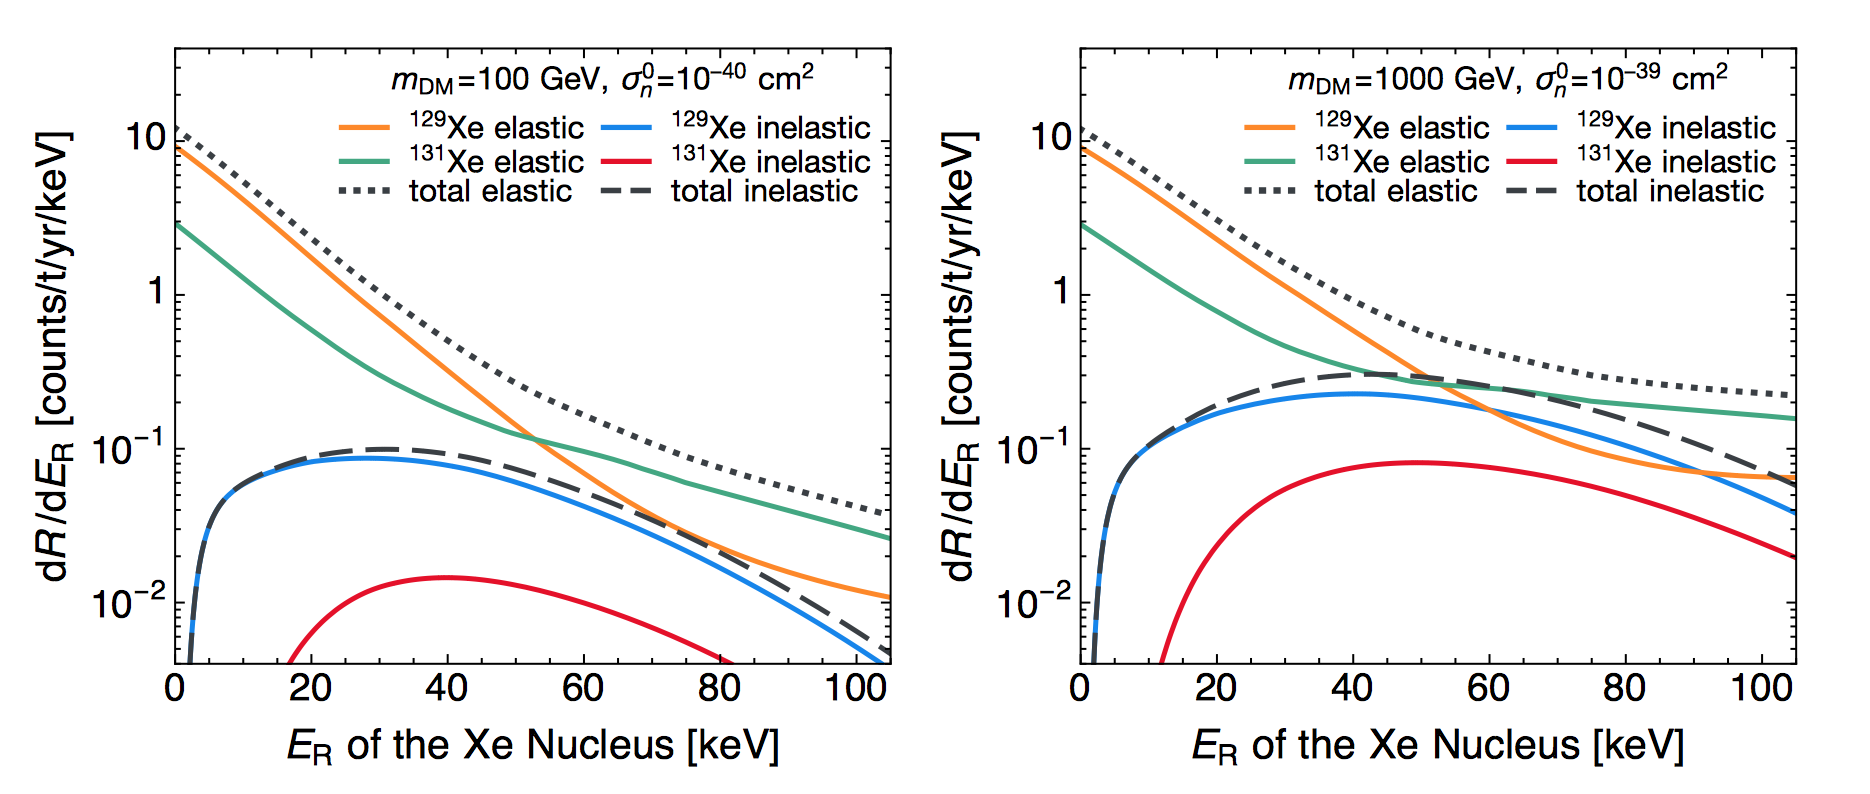
\includegraphics[width=\textwidth]{ElasticInelasticRates}
\caption{Spin-dependent recoil spectra for \ce{^{129}Xe} and \ce{^{131}Xe} for elastic and inelastic scatters.  WIMP masses
of of $100\ \mathrm{GeV/c^2}$ with cross section $\sigma_{n}^{0} = 10^{-40}\ \mathrm{cm^{2}}$
and $1000\ \mathrm{GeV/c^2}$ with cross section $\sigma_{n}^{0} = 10^{-39}\ \mathrm{cm^{2}}$ are assumed.  Elastic scattering
is preferred across all recoil energies, though at larger $E_{\mathrm{R}}$ and $m_{\chi}$ inelastic has a greater relative
impact.  Inelastic scattering drops to 0 at 
$E_{R} = 0\ \mathrm{keV}$ because conservation of momentum mandates that the nucleus cannot be excited while the atom remains at rest
after an interaction.  Image credit: \citeref{McCabe2016}.}
\label{fig:nr_elastic_inelastic}
\end{figure}

The final kind of interaction is elastic scattering and preserves kinetic energy.  Elastic scatters probe both spin-independence
and spin-dependence.  \figref{fig:nr_elastic_inelastic} shows the expected recoil spectra for \ce{^{129}Xe} and
\ce{^{131}Xe} elastic and
inelastic scatterings for WIMPs of $m_{\chi} = 100,\ 1000\ \mathrm{GeV/c^2}$ with cross-sections of
$\sigma_{n}^{0} = 10^{-40},\ 10^{-39}\ \mathrm{cm^{2}}$.  We see that elastic scattering is dominant over inelastic, but at higher recoil
energies $E_{R}$ and larger WIMP masses the gap of the discrepancy decreases.  This suggests a spin-dependent dark matter discovery should
be first observed with elastic scatters.  From here on elastic scattering will be the primary focus since it is used for the
spin-independent search (a few sections will focus on $\mathrm{^{129m}Xe}$ and $\mathrm{^{131m}Xe}$).


%====================================
\section{Electronic Recoils}
\label{sec:er}
Xenon will undergo an electronic recoil when its electron shell interacts with a moving particle.  Because no energy
is lost to atomic motion the number of quanta produced is

\begin{equation}
n_{\mathrm{q}} = \frac{E}{W}
\label{eq:nquant_er}
\end{equation}

\noindent where $W = 13.7 \pm 0.2\ \mathrm{eV}$ \citeref{Dahl2009} is the energy required to produce a single quantum.  This is made up
of

\begin{equation}
n_{\mathrm{q}} = n_{\mathrm{ex}} + n_{\mathrm{ion}}
\label{eq:quanta}
\end{equation}

\noindent where \nex and \nion is the numbers of excitons and ions, respectively.  The number of electron-ion pairs has a root mean square
of

\begin{equation}
\delta = F \times n_{\mathrm{ion}}
\label{eq:fano}
\end{equation}

\noindent where $F < 1$ is known as the Fano factor \citeref{Fano1947}.  Thus the fluctuations of $n_{\mathrm{ion}}$ are smaller than a
Poisson distribution ($F = 1$).  Several experiments have attempted to measure $F$ for LXe \citeref{Doke1976, Seguinot1995} and
estimate a value of $F = 0.059$ for \electron and $\gamma$-rays.  This places a limit on the fundamental energy resolution of

\begin{equation}
\Delta E = \sqrt{F W E}
\end{equation}

\noindent where it is common to measure $\Delta E$ is in keV, $W$ is in eV, and the energy $E$ is in MeV \citeref{Aprile2009}.  Current
LXe experiments have not yet achieved a Poisson resolution, so there is a lot of progress that can be made in the future.

Rearranging \eqnref{eq:quanta} the probability that a quanta is an ion is

\begin{equation}
p_{\mathrm{ion}} = \frac{1}{1 + \frac{ n_{\mathrm{ex}} }{ n_{\mathrm{ion}} }}
\end{equation}

\noindent with $p_{\mathrm{ex}} = 1 - p_{\mathrm{ion}}$.  The ratio $n_{\mathrm{ex}} / n_{\mathrm{ion}}$ has been calculated to be
0.06 \citeref{Takahashi1975}
but later measurements disagree \citeref{Doke2002, Aprile2007}.  Currently $n_{\mathrm{ex}} / n_{\mathrm{ion}}$ is expected to be
between 0.06-0.2.  Following recombination the number of photons and electrons is

\begin{subequations}
\begin{align}
n_{\mathrm{ph}} &= n_{\mathrm{ex}} + rn_{\mathrm{ion}} \\
n_{\mathrm{e}} &= (1 - r)n_{\mathrm{ion}}
\end{align}
\end{subequations}

\noindent where \nphot is the number of photons and \nelect is the number of \electron that do not recombine.

Although noble gas detectors allow ER-NR discrimination, the two regions are near one another some events could
be considered with reasonable probability to belong to either.  In dark matter searches only the region of NR-space where the NR
likelihood is significantly more probable is used (\secref{sec:dark_matter_results}).  A number of reduction methods are used to minimize
the electronic recoil and other backgrounds.  With the ton-scale era of DM detectors
underway this becomes especially critical, and significant effort has been put into material screening and distillation.


%====================================
\section{Nuclear Recoils}
\label{sec:nr}
Although the vast majority of background comes from electronic recoils, nuclear recoils are more dangerous because they replicate
WIMP interactions.  Therefore the NR background must be well-modeled to avoid mistaking background with WIMPs.

A fraction of the energy in a nuclear recoil will increase the kinetic energy of the xenon.  Liquid noble gas detectors cannot measure
changes in translational motion of atoms so this portion is lost.  While energetic electrons are capable of transferring very small
amounts of energy to the motion of the nucleus, the reverse is not true.  Atomic motion has only been observed in nuclear recoils,
which implies for the same energy deposition $n_{\mathrm{q}}$ will differ between electronic and nuclear recoils.  The fraction of energy
not lost to atomic motion $f_{n}$ is commonly described by the Lindhard model
\citeref{Lindhard1965}

\begin{equation}
f_{n} = \frac{k g(\epsilon)}{1 + k g(\epsilon)}
\label{eq:linhard_quenching}
\end{equation}

\noindent where $k = 0.133Z^{2/3}A^{1/2}$, $g(\epsilon) = 3\epsilon^{0.15} + 0.7\epsilon^{0.6} + \epsilon$, and
$\epsilon = 11.5 (E / Z^{7/3})$ where $Z$ is the atomic number, $A$ is the number of nucleons, and $E$ has units of keV.  $k$ is
proportional to the ratio of
electronic stopping power to particle velocity of the recoiling Xe atom \citeref{Sorensen2011} and $g(\epsilon)$ is proportional
to the ratio of electronic to nuclear stopping power (\secref{subsec:stopping_power}) \citeref{NEST2015}.  Here $k$ is taken
from \citeref{Lewin1996} but there has been some debate over its value.  When parameterized by the Lindhard model the quenching factor
$f_{n}$ is sometimes written as $L(E)$.  It is shown in \figref{fig:lindhard} for the relevant energy search region.

\begin{figure}
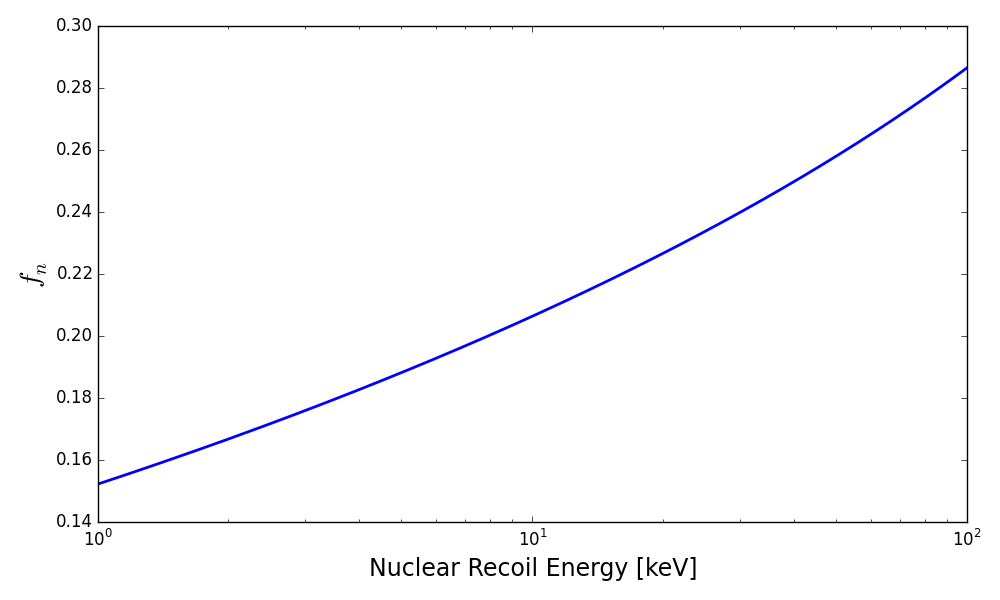
\includegraphics[width=0.8\textwidth]{Lindhard}
\caption{Fraction of nuclear recoil energy that causes excitons and ions in xenon using Lindhard's theory \citeref{Lindhard1965}.}
\label{fig:lindhard}
\end{figure}

Primary scintillation is reduced by biexcitonic quenching and the Penning process (\eqnref{eq:nr_scint_quench}).  The total
number of quanta is

\begin{equation}
n_{\mathrm{q}} = L(E) \frac{E}{W}
\label{eq:nquant_nr}
\end{equation}

\noindent The difference between \eqnref{eq:nquant_er} and \eqnref{eq:nquant_nr} is $L(E)$.  As with electronic recoils the probability
of a quantum being an ion is

\begin{equation}
p_{\mathrm{ion}} = \frac{1}{1 + \frac{ n_{\mathrm{ex}} }{ n_{\mathrm{ion}} }}
\end{equation}

\noindent through the higher track density of nuclear recoils (\figref{fig:er_nr_recoil_diagram})  causes
$n_{\mathrm{ex}} / n_{\mathrm{ion}} \sim 1$ \citeref{Sorensen2011, Angle2011}.  As electrons and ions
recombine biexcitonic quenching and the Penning process reduce the number of photons by $f_b$ (\eqnref{eq:nr_scint_quench}).

\begin{subequations}
\begin{align}
n_{\mathrm{ph}} &= f_b ( n_{\mathrm{ex}} + rn_{\mathrm{ion}} ) \\
n_{\mathrm{e}} &= (1 - r)n_{\mathrm{ion}}
\end{align}
\end{subequations}



%====================================
\section{Time Projection Chambers}
\label{sec:tpcs}
Time projection chambers (TPCs) measure the light and charge of an interaction.  They have been leading the
spin-independent search for WIMP masses $> 10\ \mathrm{GeV/c^2}$ for ${\sim}10\ \mathrm{years}$, and as we reach the ton-scale era are
projected to continue.  \figref{fig:sensitivity_evo} shows the evolution of detectors and their spin-independent limits for roughly
$30 \mdash 70\ \mathrm{GeV/c^2}$ WIMPs.  This section discusses liquid noble gas TPCs used for dark matter detection.  It primarily covers
xenon but for most details an identical treatment can be applied to argon and neon.

\begin{figure}
\centering
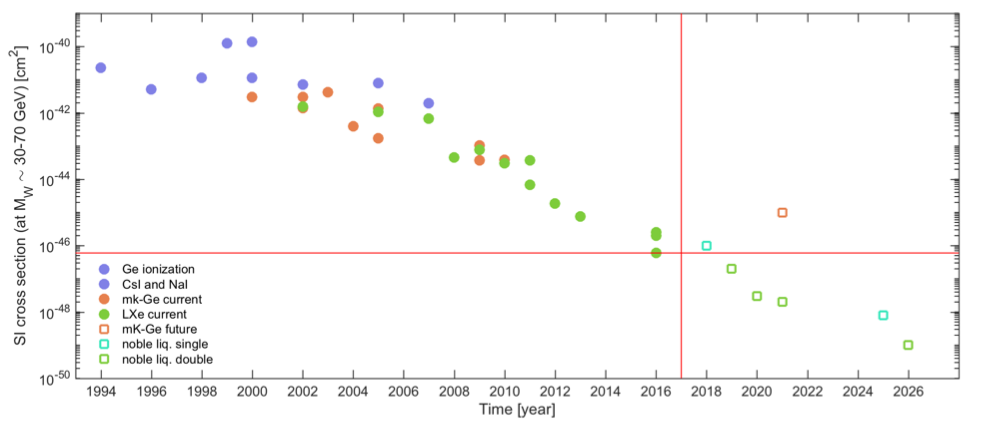
\includegraphics[width=0.9\textwidth]{SensitivityEvolutionBetter}
\caption{Spin-independent cross-section evolution for WIMPs with $m_{\chi} \sim 30 \mdash 70\ \mathrm{GeV/c^2}$.  Solid markers represent
realized
values while empty squares denote projected.  Purple markers refer to germanium (\secref{subsec:germanium}) as well as CsI and NaI
detectors (\secref{subsec:crystals}), orange represent cryogenic bolometers (\secref{subsec:bolometers}), turquoise denotes single-phase
noble liquid chambers, and green symbolizes dual-phase.  For approximately the last decade LXe detectors have led the search and are
projected to continue to do so.  Image credit: \citeref{Baudis2014}.}
% for SensitivityEvolution
%Black circles refer to germanium and silicon detectors (\secref{subsec:germanium}), blue diamonds
%depict cryogenic bolometers (\secref{subsec:bolometers}), red and green triangles symbolize LXe and LAr detectors, and
%purple squares represent bubble chambers (\secref{subsec:bubbles}).  Image credit: \citeref{Undagoitia2016}.}
\label{fig:sensitivity_evo}
\end{figure}

\subsection{Working Principle}
\label{subsec:tpcs_working_principle}
TPCs consist of a liquid noble element with a small gas gap at the top.  A minimum of three parallel metal meshes are needed: the
cathode, gate, and anode.  The cathode is
at the bottom of the detector and applies an electric field - known as the drift field $E_d$ - inside the active volume.  The gate rests
just beneath the liquid level and is grounded, so the drift field pushes electrons that do not recombine towards the surface of the liquid
at drift velocity $v_{d}$.  Typically an electric field cage consists
of metal rings that mark the perimeter and are stacked vertically, parallel to the cathode and gate.  Identical resistors connect adjacent
rings so voltage drops are equivalent and maintain drift field uniformity.

The observable that corresponds to the measurement of photons emitted from the site of the interaction is referred to as the S1, named
because it is the first scintillation.  The electrons, which do not contribute to the S1, drift to the surface of the liquid.  Over this
period the electron cloud diffuses longitudinally (in the direction of $E_{d}$) and transversely (perpendicular).  The
diffusion coefficients $D_{L}$ and $D_{T}$ are dependent on the electric field with $D_{T}/D_{L} \sim 10$.  The electron spread can
be written as $\sigma_{D_{T}} = \sqrt{D_{T} t_{d}}$ where $t_{d} = d/v_{d}$ is the electron drift time and $d$ is the drift distance.

Impurities that outgas from detector materials mix into the gas and liquid.  Electronegative impurities in particular are a problem
because they attach to drifting $e^{-}$ and
lower the number that reach the liquid-gas interface.  The attachment process
is \eqnref{eq:impurity_attach}.

\begin{equation}
e^{-} + S \rightarrow S^{-}
\label{eq:impurity_attach}
\end{equation}

\noindent where $S$ is an impurity.  The number of \electron captured depends on drift time and the impurity attachment rate
$k_{S}$, both of which vary with $E_{d}$.  An advantage of larger electric fields is a greater
\vd (up to a point, \figref{fig:drift_velocity}) to limit time in the liquid.  Doping LXe with organic materials such as butane
can increase \vd at large
fields but are not used in DM detectors because of purification difficulties \citeref{Yoshino1976}.  The rate at which electrons are
absorbed by impurities is proportional to the number of electrons, impurities, and impurity attachment rate.  Assuming the density
of impurities in the liquid and $E_{d}$ are uniform the charge $q$ is described by

\begin{equation}
\frac{dq}{dt} = -qk_{S}S
\label{eq:lifetime_diff_eq}
\end{equation}

\begin{equation}
q(t) = q_{0}e^{-tk_{S}S} = q_{0}e^{-t/\tau_{e}}
\label{eq:lifetime_equation}
\end{equation}

\noindent where $\tau_{e} = (k_{S}S)^{-1}$ is the electron lifetime and $q_0$ is the initial charge.  $k_{S}$ is the attaching rate
constant and is shown in \figref{fig:attachment_rate} for O$_{2}$,
N$_{2}$O, and SF$_{6}$.  It increases for N$_{2}$O with $E_d$ whereas \otwo and SF$_{6}$
decerase.  For LXe TPCs it is common to give the impurity concentration in \ce{O_2}-equivalence - the concentration of \otwo if it were
solely responsible for \electron attachment.  \ce{O_2} is expected to be the dominant electronegative contaminant, and its curve
in \figref{fig:attachment_rate} works well for modeling the electron lifetime (\chapref{chap:purification}).  Removing these
impurities is discussed in \secref{subsec:xenon1t_pur} and measuring the electron lifetime is covered in
\secref{subsec:det_char_elifetime, sec:electron_lifetime_measurements}.

\begin{figure}
\includegraphics[width=0.8\textwidth]{attachingratevsfield}
\caption{Attaching rate constant $k_{S}$ for O$_{2}$, N$_{2}$O, and SF$_{6}$ with respect to electric field.  At
larger $E_d$ $k_{S}$ increases for N$_{2}$O and decreases for \otwo and SF$_{6}$.  Image credit: \citeref{Bakale1976}.}
\label{fig:attachment_rate}
\end{figure}

The anode rests several millimeters above the gate.  The electric field between the gate and anode $E_{g}$ must be strong
enough to extract the \electron that reach the liquid surface into the gas (typically $\gtrsim 10\ \mathrm{kV\ cm^{-1}}$).  An extracted
\electron will quickly gain enough kinetic energy to ionize atoms in the gas,
whose \electron in turn follow, creating a cascade effect.  Because the scintillation per electron is independent of
the total number of electrons extracted this is known as proportional scintillation.  It is also known as secondary scintillation or
electroluminescence.  The number of photons $N_{\mathrm{ph}}$ produced over a distance $z$ per electron is

\begin{equation}
\frac{dN_{\mathrm{ph}}}{dz} = \alpha \bigg( \frac{E_{g}}{P} - \beta \bigg) P
\label{eq:electronlum}
\end{equation}

\noindent where $\alpha = 70\ \mathrm{photons\ kV^{-1}}$, $\beta = 1.0\ \mathrm{kV\ cm^{-1}\ atm^{-1}}$, and $P$ is the pressure in the
gas \citeref{Belogurov1995}.  The observable that corresponds to the measurement of electroluminescence is referred to as the S2, for
second scintillation.


\subsection{Photomultiplier Tubes}
\label{subsec:tpcs_pmts}
Photomultiplier tubes (PMTs) are used for light detection in TPCs.  A digram of a PMT is shown in \figref{fig:tpcs_pmts_pmt_diagram}.  A
photon that
passes through the PMT window will most often strike the photocathode and free a photoelectron via the photoelectric effect.  This process
is known as single photoelectron emission (SPE).  Once ejected, the photoelectron will be directed by the focusing electrode towards the
first dynode.  The dynodes are coupled to one another through resistors that systematically decrease their electric potential.  As the
photoelectron hits the first dynode it will free a second electron.  The freed electrons will be drawn to the
second dynode and repeat this procedure.  The result is a cascade effect, amplifying the current by as much as 100 million and ending
at the anode, where the charge is output to a voltage reading device such as an oscilloscope or digitizer.

\begin{figure}
\centering
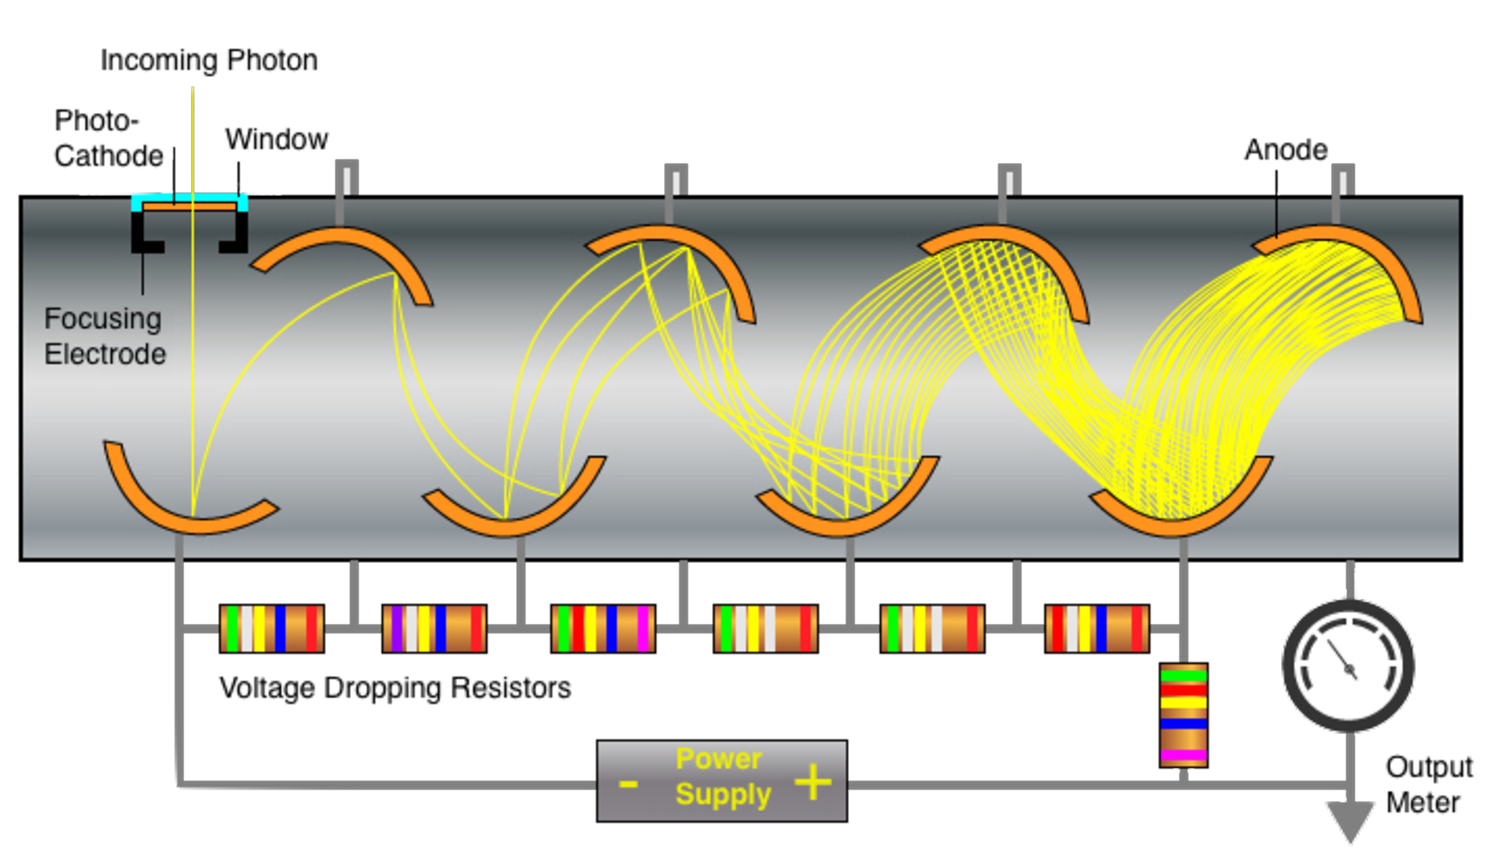
\includegraphics[width=0.8\textwidth]{PMT1Better}
\caption{Diagram of a PMT.  An incident photon hits the photocathode and ejects an photoelectron.  With each dynode the more \electron are
freed, creating an amplified signal.  Image credit: \citeref{CHROMacademy}.}
\label{fig:tpcs_pmts_pmt_diagram}
\end{figure}

If the photon's energy is at least double the workfunction of the photocathode the number of photoelectrons ejected should follow
follow a Poisson distribution.  However, a study of several Hamamatsu vacuum ultraviolet-sensitive (VUV) PMTs showed double
photoelectron emission
(DPE) fractions between 18-24\% depending on the PMT, higher than the expected ${\sim} 15\%$ \citeref{Faham2015}.  The study included PMTs
used in XENON100 and XENON1T.  In other cases a photon may pass through the photocathode and hit
the first dynode.  If it ejects an electron the PMT response
will be similar to a photocathode hit with one less dynode, i.e. an under-amplified current.  

The quantum efficiency (QE) is the ratio of electrons ejected from the photocathode divided by incident photons.  The QE spectrum for
the PMTs used in XENON1T, Hamamatsu R11410, is shown in \figref{fig:tpcs_pmts_qe}.  Its low efficiency means the majority of photons that
reach our PMTs will not produce a photoelectron.  Other photodetectors have been considered but lead to problems that outweigh those
of PMTs.  Xenon's scintillation wavelength (178 nm) is near the spectrum's maximum of approximately 35\%.  Liquid argon and neon have
scintillation wavelengths of 128 and 78 nm, respectively.  Because PMTs are not sensitive to these energies LAr experiments use
wavelength shifters.

\begin{figure}
\centering
\includegraphics[width=0.6\textwidth]{pmt_efficiency}
\caption{Quantum efficiency with respect to wavelength for the Hamamatsu R11410 PMT, used in XENON1T.  The peak efficiency occurs near
the xenon scintillation wavelength 178 nm at ${\sim} 35 \%$.  Image credit: \citeref{Lung2012}.}
\label{fig:tpcs_pmts_qe}
\end{figure}

TPCs have photomultiplier tubes below the cathode and above the gate.  While proportional scintillation occurs at the top of the detector
and in most detector settings produces enough light to guarantee detection, prompt scintillation - especially for low energy events - can
be more difficult to observe.  Depending on the geometry of the detector and the location of the event the fraction of light
directed towards the photodetectors can
be small.  PMTs cannot be fixed around the side of the TPC because their electric fields will interfere with the field
cage.  To increase
the fraction of light that reaches the photodetectors the wall of the TPC is covered by polytetrafluoroethylene (PTFE) just inside the
field cage.  PTFE is reflective for liquid noble gas scintillation and is a common choice.  It has been shown to have $> 97 \%$
reflectance to 178 nm light when immersed in LXe \citeref{Neves2017}.



\subsection{Signals}
\label{subsec:tpcs_signals}
S1s (primary scintillation) and S2s (secondary) are measured in photoelectrons (PEs).  An example of an
event is shown in \figref{fig:tpcs_signal_tpc}.  On the left a particle scatters with the LXe, prompting photons that are almost
immediately observed by the PMTs.  The right side shows the \electron drifting to the LXe surface and
extracted by the anode across the GXe.  The colors correspond to the relative intensity of light seen by each PMT.  For a typical S1 the
bottom PMTs observe more light due to reflection off the LXe surface (though the amount depends on where in the TPC the interaction
occurs).  For S2s the top PMTs see more light since electroluminescence occurs just several centimeters underneath them.  For S2s
the top PMTs have an intensity profile centered around where the \electron are extracted.  The profile for the bottom PMTs is more
uniform since the solid angle per PMT is less.

\begin{figure}
\centering
\includegraphics[width=\textwidth]{xenon1t_tpc}
\caption{Diagram of an interaction in a LXe TPC.  The S1 is immediately
observed by the PMTs.  The \electron drift towards the top of the detector, where they are extracted across GXe,
creating the S2.  A typical waveform is shown at the bottom.  The S2 is significantly
larger than the S1 due to the amplification of electroluminescence.  The relative intensity of light in the PMTs, or PMT hit
pattern, can be used to determine the $x$- and $y$-coordinates of the interaction.  Image credit: Lutz Alth\"{u}ser.}
\label{fig:tpcs_signal_tpc}
\end{figure}



\subsubsection{Position Reconstruction}
\label{subsubsec:tpcs_signals_posrec}
In addition to knowing the $z$-coordinate of the interaction ($z = v_{d} t_{d}$) TPCs can recover the $x$ and $y$ positions.  The S2
hit pattern in the top PMT array in \figref{fig:tpcs_signal_tpc} shows an intensity distribution that peaks at one
PMT and dissipates away from it.  It is reasonable to assume the S2 was extracted beneath or nearly beneath this PMT.  A number of
algorithms can be applied to PMT hit patterns to estimate the $x \mdash y$ position of the event.  Typically the resolution of event
reconstruction depends on the number and area of PMTs as well as the S2 size.  \figref{fig:tpcs_signals_posrec} shows the event
distribution for second XENON1T science run.  The majority of events are near the wall - a consequence of
radioactivity present in detector materials.  The large self-shielding of LXe constrains these events to ${\sim}5\ \mathrm{cm}$ of the
wall.  Three-dimensional position reconstruction allows us to reject events in regions where we
expect a large background.  The region of interest for dark matter search data is known as the fiducial volume.

\begin{figure}
    \centering
    \begin{subfigure}[t]{0.45\textwidth}
        \centering
        \includegraphics[height=4.5cm]{PosRecXY}
    \end{subfigure}%
    \begin{subfigure}[t]{0.45\textwidth}
        \centering
        \includegraphics[height=4.5cm]{PosRecRZ}
    \end{subfigure}
    \caption{Position reconstruction for events in XENON1T Science Run 1.  Top PMT hit patterns are used to determine $x \mdash y$ while
    $z = v_{d} t_{d}$.  The number of events drops dramatically at lower radii due to the self-shielding of LXe.}
	\label{fig:tpcs_signals_posrec}
\end{figure}



\subsubsection{Discrimination}
\label{subsubsec:tpcs_signals_discr}
The exciton-to-ion ratio and recombination (\secref{subsec:recombination}) are responsible for the fraction of quanta that produce S1s
and S2s.  Under identical
detector conditions recombination is largely governed by the ionization density, which is determined by the stopping power
(\secref{subsec:stopping_power}).  \figref{fig:mass_stopping_power} shows the mass stopping power dependence on energy and recoil type,
and \figref{fig:er_nr_recoil_diagram} shows the track structure for 20 keV electronic and nuclear recoils.  Because the nuclear recoil has
a greater ionization density its electron-ion pairs are more likely to recombine \citeref{Faham2014}.  The disproportionate exciton-to-ion
ratios and recombination fraction allow discrimination between electronic and nuclear recoils.

\figref{fig:tpcs_signals_ernr} shows S2 vs. S1 for electronic and nuclear recoils.  The ER are from \ce{^{220}Rn} calibrations
where its progeny \ce{^{212}Pb} undergoes $\beta$-decay.  The short lifetime of the \ce{^{220}Rn} decay chain, continuous energy spectrum
of $\beta$-decays, and uniform distribution throughout the detector make \ce{^{220}Rn} an excellent choice for measuring S1 and S2 for
electronic recoils.

To map the S1-S2 parameter spaces separate ER and NR calibrations are performed.  Electron recoil calibrations use \ce{^{220}Rn} since
its progeny \ce{^{212}Pb} undergoes $\beta$-decay.  The short lifetime of the \ce{^{220}Rn} decay chain
($\sum_i t_{1/2} < 12\ \mathrm{h}$), continuous energy spectrum
of $\beta$-decays, and uniform distribution throughout the detector make it an excellent choice for measuring S1 and S2 for
electronic recoils.  Events from XENON1T calibrations are shown in red in \figref{fig:tpcs_signals_ernr}.

There are no neutron sources that can be mixed with xenon to perform internal nuclear recoil calibrations.  Therefore, calibrations
must be done with sources placed outside of the detector.  Xenon's self-shielding (${\sim}10\ \mathrm{rm}$ mean free path for MeV
neutrons \citeref{Israelashvili2015}) causes the distribution of events to be largest near
the source, and - depending on the size of the detector - can significantly reduce the fraction of events that reach the center of the
detector, and force longer calibration windows.  For XENON1T nuclear recoil sources include
americium beryllium \ce{^{241}AmBe} and a deuterium-deuterium (D-D) neutron generator (NG) \citeref{Lang2018}.  The nuclear recoils are
marked in blue in \figref{fig:tpcs_signals_ernr} are from the \ambe calibration during the second XENON1T science run.

As predicted above \figref{fig:tpcs_signals_ernr} shows nuclear recoils have a larger photon-to-electron ratio than electronic recoils due
to their higher $n_{\mathrm{ex}}/n_{\mathrm{ion}}$ and recombination.  It shows

\begin{equation}
\bigg( \frac{\mathrm{S}2}{\mathrm{S}1} \bigg)_{\mathrm{ER}} > \bigg( \frac{\mathrm{S}2}{\mathrm{S}1} \bigg)_{\mathrm{NR}}
\end{equation}

\noindent across all S1-S2 values.  This data is used to characterize the ER and NR observables (S1, S2) space so that the origin of each
dark
matter search event can be estimated.  Because a substantial fraction of energy is lost to atomic motion in a nuclear recoil the energies
of the events in \figref{fig:tpcs_signals_ernr} differ between ER and NR.  As an example, a nuclear recoil event at
$\mathrm{S1} = 60\ \mathrm{PE}$ has an energy of ${\sim}35\ \mathrm{keV}$ while for electronic recoils it is closer to 8 keV.  For this
reason several energy scales are used (\secref{subsubsec:tpcs_signals_energy}).

\begin{figure}
\centering
\includegraphics[width=\textwidth]{er_nr_discrimination}
\caption{S2 (proportional) vs. S1 (prompt) for XENON1T calibration data.  Electronic recoils are from the \ce{^{220}Rn} decay chain as
progeny \ce{^{212}Pb} undergoes $\beta$-decay with an end-point energy of 569.9 keV (red).  Nuclear
recoils are from americium beryllium (\ce{^{241}AmBe}) (blue).  S2/S1 is larger for electronic recoils, which enables discrimination
between possible WIMPs and the ER background.}
\label{fig:tpcs_signals_ernr}
\end{figure}

The number of photons and electrons can be reconstructed from the S1 and S2.  Doing so requires knowledge of a number of detector
variables including PMT quantum efficiencies (\secref{subsec:tpcs_pmts}) and electroluminescence
(\secref{subsec:tpcs_working_principle}).  These are discussed in detail in \secref{sec:det_char} and
\secref{sec:er_nr_calibrations_parameter_determ}.  If the energy of an event is known the light yield and charge yield can be calculated
in units of photons per energy and electrons per energy, i.e. $n_{\mathrm{phot}}/E$ and $n_{\mathrm{e}}/E$.  Because the light and charge
yields describe detector-independent microphysics there has been an effort to measure them
(\secref{sec:er_nr_calibrations_results_ly_qy}).  Measurements of photoelectrons per energy may also be referred to as light and charge
yields (\secref{subsec:det_char_ly_cy}) and are useful for monitoring detector conditions (because they are detector-dependent they do not
provide insight into fundamental physics).  \figref{fig:tpcs_signals_drift_field} shows the ratios of light and
charge yields as a function of drift field for 122 keV electronic recoils (\ce{^{57}Co} $\gamma$-rays), 56.5 keV elastic nuclear recoils
(\ce{^{241}AmBe} and \ce{^{252Cf}}), and
5.3 MeV $\alpha$-decays (\ce{^{210}Po}).  At larger $E_d$ the light yield declines while the charge yield increases.  The more
significant change in ER is due to its sparser ionization density and suggests the drift field can be optimized for ER-NR discrimination.

\begin{figure}
\centering
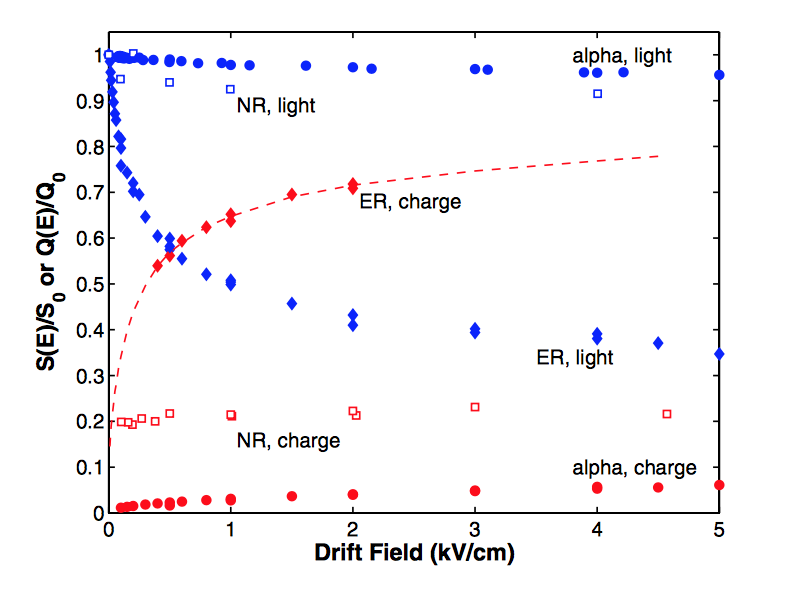
\includegraphics[width=0.8\textwidth]{LYQY}
\caption{Field dependence of light (S(E)/S$_{0}$, red) and charge (Q(E)/Q$_{0}$, blue) yields.  S$_{0}$ is the light yield at zero field
and Q$_{0}$ is the charge yield at
infinite field.  Electronic recoils are shown as solid diamonds and are measured from \ce{^{57}Co} 122 keV $\gamma$-rays.  56.5
keV elastic neutron scatters from \ambe and \ce{^{252}Cf} are marked by hollow squares.Nuclear recoils
are marked by hollow squares and are from elastic 56.5 keV neutron scatters from \ambe and \ce{^{252}Cf}.  Solid circles represent \ce{^{210}Po}
5.3 MeV $\alpha$-decays.  Sparser ionization densities precipitate stronger field-dependence for electronic scatters than for nuclear and
alpha, signifying $E_{d}$ can be tuned for improved ER-NR discrimination.  Image credit: \citeref{Aprile2006b}.}
\label{fig:tpcs_signals_drift_field}
\end{figure}



\subsubsection{Energy Reconstruction}
\label{subsubsec:tpcs_signals_energy}
An important feature in a detector is the ability reconstruct the energy of the event.  There are several energy scales used
depending on the interest.  For electronic recoils energy
reconstruction is relatively straightforward since the energy is converted to photons and electrons.  Nuclear recoils are more
complicated since they pick up translational energy and are more likely to undergo biexcitonic quenching.  There are three commonly-used
energy scales.

The \textbf{electronic recoil equivalent energy} is the name for conversion between \gammaray and detector response of scintillation or
ionization, generally measured in PE.  It can be used to identify mono-energetic $\gamma$ lines, which are useful im defining the energy
scale.  If only the S1 or S2 is measured the energy is typically specified since the recombination fraction varies with energy.  The units
are given as ``$\mathrm{keV_{ee}}$'' for electron-equivalent.

The \textbf{electron equivalent combined energy scale (CES)} uses the primary and proportional scintillations to reconstruct $E$.  This is
only used for electronic recoils since, unlike nuclear recoils, energy is not lost to xenon nuclei (either as kinetic energy or nuclear
excitation).  Using this scale we can reconstruct our background energy spectrum (ERs are $> 99\%$ of total background).

The ``electron-recoil equivalent energy" scale is used for the conversion of signal to energy using $\gamma$-rays.  It uses either the S1 or
S2 and has units of photoelectrons or electrons, respectively.  It has units of $\mathrm{keV_{ee}}$ for ``electron-equivalent".  Because
recombination varies with respect to energy this scale will be non-linear, so it is common to include the energy used in the
calibration.

``Nuclear-recoil equivalent energy" is based on nuclear recoil primary scintillation.  For historical reasons it is defined using the
122 keV \gammaray from \ce{^{57}Co}.  It is given by

\begin{equation}
E_{\mathrm{NR}} = \frac{S1 S_{\mathrm{ER}}(E)}{L_{y,\mathrm{ER}} \mathcal{L}_{eff} S_{\mathrm{NR}}(E)}
\end{equation}

\noindent where $L_{y,\mathrm{ER}}$ is the electronic recoil light yield at 122 keV, $\mathcal{L}_{eff}$ is the relative nuclear
recoil
scintillation efficiency, and $S_{\mathrm{ER,NR}}(E)$ are the scintillation quenching factors for ER and NR, respectively.  Units are
given in \kevnr for ``nuclear-equivalent".

The ``combined energy scale" uses both S1 and S2.  This is beneficial because natural fluctuations between photons and electrons at a
given energy are now accounted for (\eqnref{eq:nphot_ne}).  In addition it typically leads to better energy resolution because both signals
are used, and recombination variation over energy does not lead to non-linearity.  Typically several $\gamma$ sources are used to
construct it, so it takes units of $\mathrm{keV_{ee}}$.






















% for stopping power look at A Model of Nuclear Recoil Scintillation Efficiency in Noble Liquids
%D.-M. Mei a,∗ Z.-B. Yin a,b,1, L.C. Stonehill c, A. Hime c


%Lewin and Smith (1996) - Lindhard factor
%Doke et al., 2002 - LET
%Miller et al., 1968 - drift velocity








% for kr/xe level
%E Aprile, J Aalbers, F Agostini, M Alfonsi, F. Amaro, M Anthony, F Arneodo, P Barrow, L Baudis, B. Bauermeister, et al., “Removing krypton from xenon by cryogenic distillation to the ppq level,” The European Physical Journal C, vol. 77, no. 5, p. 275, 2017.
%This is the third chapter of the dissertation

%The following command starts your chapter. If you want different titles used in your ToC and at the top of the page throughout the chapter, you can specify those values here. Since Columbia doesn't want extra information in the headers and footers, the "Top of Page Title" value won't actually appear.

\pagestyle{cu}
\graphicspath{{./Chapter3/Figures/}}
\chapter[The XENON1T Dark Matter Search][The XENON1T Dark Matter Search]{The XENON1T Dark Matter Search}

% https://arxiv.org/pdf/1801.07231.pdf for electron emission from wires


XENON1T is the third generation experiment of the XENON collaboration.  With a fiducial mass of $> 1000\ \mathrm{kg}$ it is the first
liquid xenon dark matter detector to reach the ton-scale era of DM detection.  Its large target mass and low radioactive background
makes it the most sensitive detector to spin-independent WIMPs.

In this chapter I describe the XENON1T experiment (\secref{sec:xenon1t_detector}) and discuss the procedure, strategy, and results of the
two dark matter runs in a run-combination analysis (\secref{sec:xenon1t_sr1}).  Original results from the first science run, or Science
Run 0 (SR0) can
be found in \citeref{Aprile2017f} and are referred to in this chapter as ``First Results'' or ``SR0-only'' but the analysis is not
discussed.  This chapter focuses on the analysis of the first and second science runs - Science Run 0 and Science Run 1
(SR0 + SR1) - referred to as ``run combination (RC)''.  Thus the data used in our First Results is re-analyzed together with new data
from SR1.

Lots of good info in Aprile2017b (instrument paper).

\section{The XENON1T Detector}
\label{sec:xenon1t_detector}




\subsection{PMTs}
\label{subsec:xenon1t_pmts}
A total of 248 Hamamatsu R11410-21 PMTs are installed in XENON1T.  The 127 PMTs in the top array are placed in a radial distribution to
maximize resolution of $r$ position reconstruction (\secref{subsec:det_char_position_reconstruction}).  The 121 in the bottom array
are packed as densely as possible to maximize light collection.  The most important characteristic of a PMT is its quantum efficiency
(QE), or the ratio of photoelectrons (electrons produced in the photocathode) divided by number of incident photons.  The R11410 window is
76.2 mm in diameter and the photocathode yields an average quantum efficiency to 178 nm of 34.5\% with 2.8\%
standard deviation (\citeref{Aprile2017b, Barrow2017}).

PMTs with the highest QE are placed in the bottom array while those with the lowest are stationed along the outside of the
top.  The difference in arrangement is strategic.  Due to liquid xenon's relatively large dielectric constant (1.95) an S1 will
often reflect off the surface and be redirected towards the bottom of the TPC.  For low-energy events - the relevant range for WIMP DM
searches - a nuclear recoils may only emit a small number ($\lesssim 100$) of photons, many of which never reach the PMTs.  Thus it is
most advantageous to position those with the highest quantum efficiency in the region most likely to see scintillation from an
S1.  Likewise, S2s easily produce enough scintillation to be observed by both arrays.  Therefore the QE of the top PMTs is comparatively
unimportant, and may even be advantageous for larger S2s where saturation can occur.  The layout of the PMTs with respect to QE is shown
in \figref{fig:xenon1t_pmt_qe}.

\begin{figure}
\centering
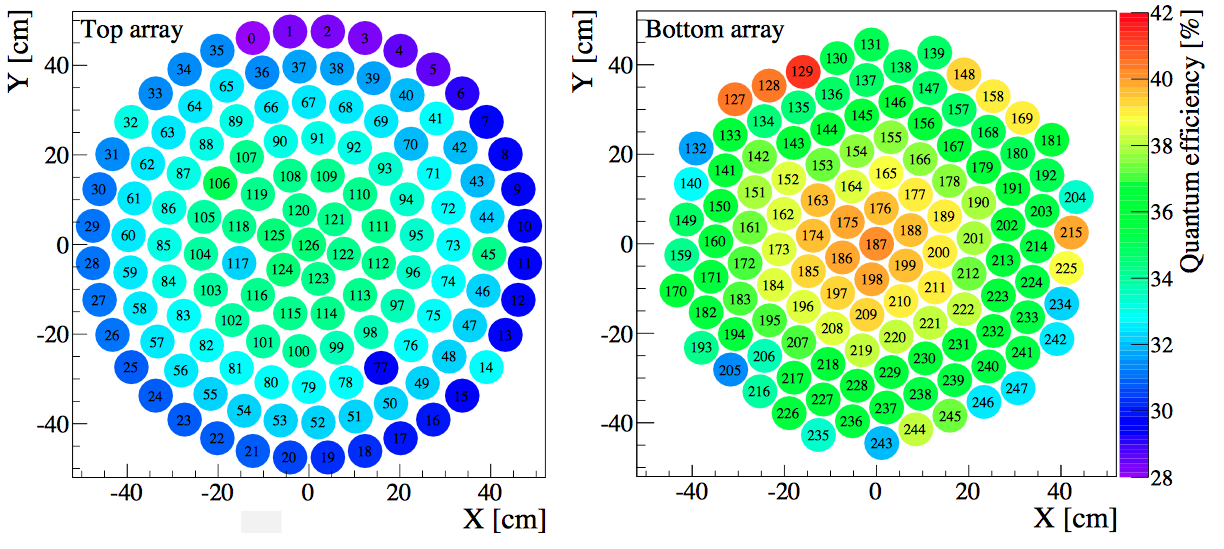
\includegraphics[width=\textwidth]{PMTQuantumEfficiency}
\caption{Quantum efficiency of top (left) and bottom (right) PMT arrays.  PMTs with highest QE are placed in the center of the bottom
array to maximize light collection while those with the lowest are placed in the outer region of the top.  Image credit:
\citeref{Aprile2017b}.}
\label{fig:xenon1t_pmt_qe}
\end{figure}

The two PMT arrays are supported by oxygen-free high thermal conductivity (OFHC) copper, with holes in which the PMTs are placed.  The
copper is then covered with polytetrafluoroethylene (PTFE) on the TPC-facing sides.  Screening meshes are situated between the bottom
array and cathode as well as the anode and top array.  Each can be biased to minimize electrical interference between the
phototubes and the drift and extraction fields.  While \citeref{Baudis2013} showed normal operation of R11410 PMTs at
$\geq 11\ \mathrm{kV\ cm^{-1}}$ the expected voltage for the cathode was $10 \mdash 100\ \mathrm{kV\ cm^{-1}}$ and decreasing the stress
on the phototubes is likely to be beneficial longterm.  The finished arrays are shown in \figref{fig:xenon1t_pmt_array}.

\begin{figure}
    \centering
    \begin{subfigure}[t]{0.5\textwidth}
        \centering
        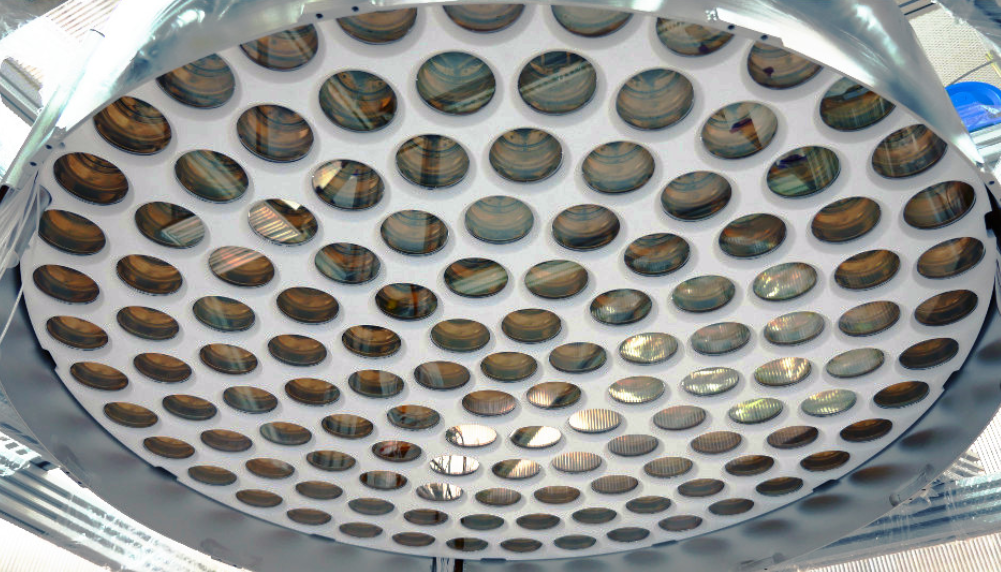
\includegraphics[height=4cm, left]{PMTTopArray}
    \end{subfigure}%
    \begin{subfigure}[t]{0.5\textwidth}
        \centering
        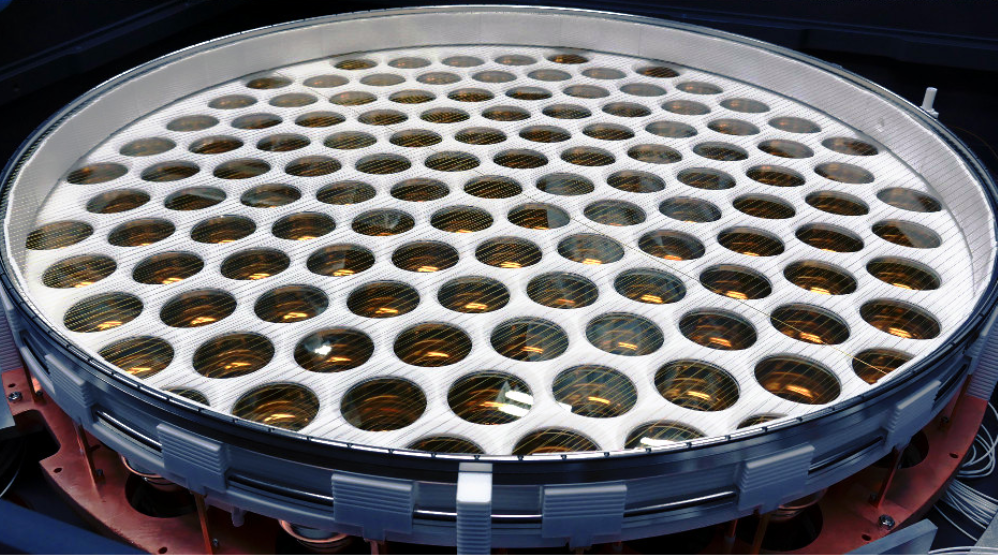
\includegraphics[height=4cm, right]{PMTBottomArray}
    \end{subfigure}
    \caption{XENON1T top (left) and bottom (right) PMT arrays.  Top PMTs are installed inside the diving bell in a radial distribution
    to minimize uncertainty in radial position reconstruction.  Bottom PMTs are installed below the cathode and screening mesh that
    limits interference between the PMT and cathode electric fields, both of which can be seen.  They are packed tightly
    together to maximize light collection.  Image credit: \citeref{Aprile2017b}.}
	\label{fig:xenon1t_pmt_array}
\end{figure}

\begin{figure}
\centering
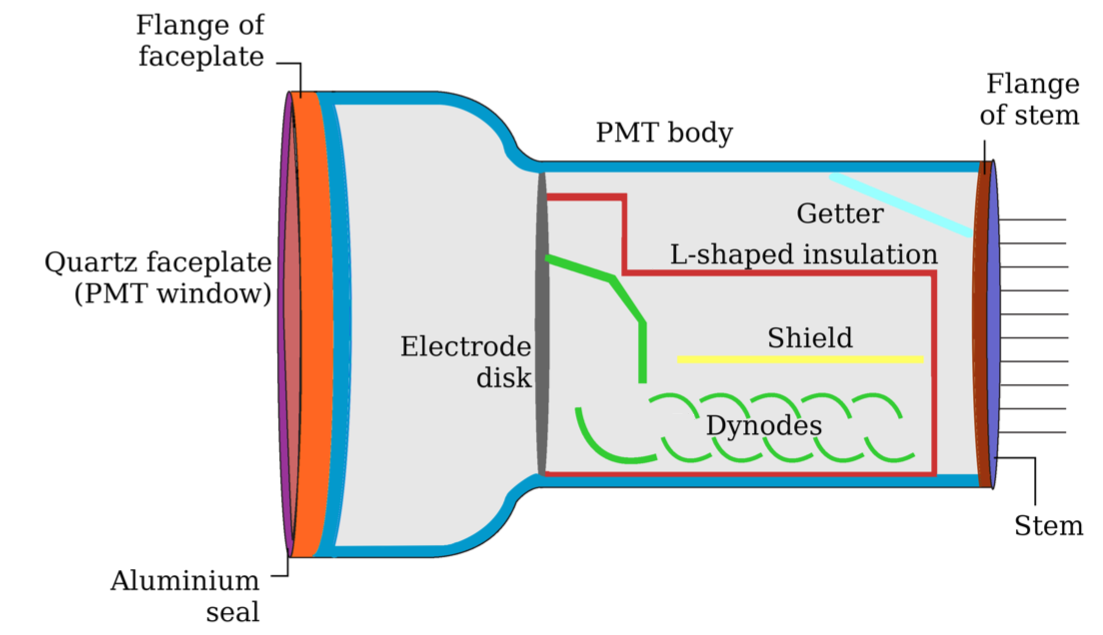
\includegraphics[width=0.8\textwidth]{PMTSchematic}
\caption{Schematic of the R11410-21 PMT.}
\label{fig:xenon1t_hamamatsu_pmt}
\end{figure}

The R11410-21 has 12 dynodes following the focusing electrode disk.  The first dynode is the largest and extends to the electrode to
maximize the probability of capturing photoelectrons.  A schematic can be be seen in \figref{fig:xenon1t_hamamatsu_pmt}.  The electrode,
dynode, and shield are stainless steel and are insulated with L-shaped quartz plates.  The window is
also made of quartz, since it is transparent to vacuum ultraviolet (VUV) photons.  Deposited on it is a low-temperature bialkali
photocathode.  The window is fixed with an aluminum seal to the faceplate flange, which along with the stem flange is constructed from
Kovar.  Because of the PMT body's large mass (71\% of total Kovar, 35\% of total) a low-\ce{^{60}Co} Kovar is chosen.  Finally, to insulate
the connections to each dynode the stem is ceramic.

Because radioactivity limits the fiducial volume and increases the event rate, making accidental coincidence and outlier events more
likely, XENON and Hamamatsu worked together to develop a highly radio-pure PMT.  There were several iterations of the R11410 model before
the R11410-21 was determined to be adequate.  Nearly all the \ce{^{137}Cs} and \ce{^{60}Co} comes from the Kovar, though the \ce{^{137}Cs}
content is negligible and the \ce{^{60}Co} is 3-10 times lower than older models.  The remaining screened isotopes, \ce{^{238}U},
\ce{^{228}Th}, \ce{^{228}Ra}, \ce{^{226}Ra}, and \ce{^{40}K}, are dominated by the ceramic stem (\citeref{Aprile2015}).  Unfortunately a
material that is more radio-pure and can insulate the dynode connections has not been found.  Sapphire was used in an iteration but
ultimately showed any improvement was minimal.

The dark count rate, or the number of signals per second above a threshold without a light source, is an important property to
characterize.  At ambient temperatures the primary cause is thermal electrons that scale with PMT voltage.  This becomes subdominant at
cryogenic temperatures to electron field emission and radioactivity (internal and external) as well as cosmic rays.  In a detector such
as XENON1T higher dark count rates make accidental coincidence more likely, which produces fake additional background and in the worst case
can place fake events in the signal region.  Because the rate is dependent on the threshold it can effectively be tuned.  However, because
for DM search we would like as low of a threshold as possible, choosing PMTs with low dark count rate is essential.

Another problematic feature is light emission from the phototube itself, where light is created inside the PMT and escapes through the
window.  It has been observed to mainly occur in one of two ways.  The first is through a discharge of intense light that can last for
several seconds.  This so-called ``flash" is bright enough to be easily observable to itself and by PMTs that are facing its
window.  However, the intensity can be so strong that it can take anywhere from several minutes to several hours for them to
recover.  Because they seem to occur spontaneously and are not well understood it is impossible to predict when a flash will occur.

The second variety is a subtle but often continuous stream of light.  Known as ``micro light emission" it is considerably harder to
identify.  Doing so requires facing two phototubes towards one another and measuring the dark rate of each one with and without the other
on.  The level of emission increases with temperature and bias voltage.  Keeping the PMTs at cryogenic temperatures during DM runs reduces
such effects, and voltages can be lowered to help further.  Still, if micro light emission continues the PMT cannot be used as it risks
contaminating the detected light from the true event population.

Directly following the pulse of a PMT hit a secondary pulse may occur.  Known as afterpulses, they can occur within 10s of
nanoseconds.  This can make them difficult to resolve from true pulses - especially S2s - that can have widths of several
microseconds.  However, they are an inevitable side effect when using PMTs so characterizing them properly is important.  There are three
mechanisms known to cause afterpulses.

The first is elastic scattering of the photoelectron with the first dynode, freeing \electron that shortly return to the dynode.  This
prompts afterpulses in the range of a few to tens of nanoseconds.  A second kind is thought to stem
from dark noise and single electrons but is not well understood.  It has a relatively uniform distribution in delay time up to several
microseconds.  Both of these afterpulses have relatively small areas of $\lesssim 2\ \mathrm{PE}$.

A photoelectron may occasionally ionize residual gas inside the PMT along its trajectory to the first dynode.  The molecule then drifts
towards the photocathode, expelling additional electrons.  The number of newly ejected electrons (area of afterpulse) depends
on the ion and the position of ionization.  The responsible ion can be determined by calculating the time between the true pulse and
afterpulse.  For R11410-21 this gives

\begin{equation}
\delta t_{\mathrm{ap}} = \frac{\pi}{4} \sqrt{\frac{2 m}{q V_{0}}} L
\end{equation}

where $\delta t_{\mathrm{ap}}$ is the delay time, $m$ and $q$ are the ion's mass and charge, and $V_{0}$ and $L$ are the potential
difference and length between the photocathode and first dynode (see \citeref{Barrow2017} for details).  Note that $\delta t_{\mathrm{ap}}$
does not depend on where the ionization occurred.  Thus, if we know the time between the true and afterpulse the ion - or more specifically
charge to mass ratio - can be calculated.  Pulse time differences range from several hundred nanoseconds to several microseconds.  These
correspond to the ``lines" in \figref{fig:xenon1t_pmts_ap} that extend to larger afterpulses.  The short timescales of S1s make them
unlikely to be grouped with an afterpulse, though for S2s this is more likely.

\begin{figure}
\centering
\includegraphics[width=\textwidth]{Afterpulse}
\caption{Afterpulses for one of the PMTs from XENON1T.}
\label{fig:xenon1t_pmts_ap}
\end{figure}

Because it is not possible to remove all residual gas any PMT will suffer from some ionization-based afterpulsing.  A better vacuum
corresponds to fewer afterpulses and a healthier PMT in general.  If the concentration of gas in the PMT vacuum were to increase it would
escalate the afterpulse rate.  Therefore if when using in xenon the Xe peaks grow over time the PMT most likely has a leak and should
be removed, as continued worsening of the vacuum will lead to deterioration and inability to operate the PMT.  All PMTs were tested before
being installed in XENON1T.  73 were rejected and replaced: 12 due to high dark count rates, 53 for light emission, and 8 for
afterpulsing.

The transit time (TT) is the time between the freed photoelectron and the arrival of the electron avalanche at the anode.  Variations in
the photoelectron's initial position as well as emitted velocity and angle cause deviations in the TT, which is characterized by the
transit time spread (TTS).  Because an event is observed by many PMTs the TTS quantifies how close together there signals should be.  Thus
smaller TTSs lead to a smaller integration window, decreasing accidental coincidence.  The TTS for all R11410-21 PMTs was measured, giving
a mean of $9.1 \pm 1.3\ \mathrm{ns}$ - a fraction of an S1.

It was shown by \citeref{Faham2015} that the probability of double photoelectron emission (DPE) in a number of PMTs, including the
R11410, is generally in the range of 0.18-0.24 - much higher than previously thought.  For The R11410 in particular they found the
probability to be $p_{\mathrm{dpe}} = 0.225 \pm 0.01$.  Any $p_{\mathrm{dpe}} > 0$ has some effect on a number of elements in a DM
search - however, with such a large value these cannot be ignored.  First it may be useful to define a second quantity closely
related to but not the same as the QE.  Following \citeref{Faham2015} the QE will be denoted as $\eta_{\mathrm{\mu}}$ and the fraction of
incident photons that produce one or more photoelectrons denoted $\eta_{\mathrm{p}}$.  Then they are related to one another by

\begin{equation}
\eta_{\mathrm{\mu}} = (1 + p_{\mathrm{dpe}}) \eta_{\mathrm{p}}
\label{eq:xenon1t_pmts_dpe}
\end{equation}

\noindent and we see that the measured QE alone will be misleading.  For one, it is common to require a PMT coincidence for an event to
be considered good - that is, $n$ PMTs must see a signal within a predetermined time window.  Using $\eta_{\mathrm{\mu}}$ will
\textit{overestimate} the likelihood of this happening, and $\eta_{\mathrm{p}}$ should instead be used.  Additionally, when the PMT
response is easily over threshold DPEs lead to incorrect resolution and yields unless accounted for.  In
\secref{subsubsec:er_nr_calibrations_parameter_determ_det_phys} during the electronic and recoil band fitting details on how to
appropriately account for all of these effects are shown.

An additional six Hamamatsu R8520 PMTs reside in LXe outside the TPC near the top electrode for studying calibrations.  These PMTs have
been used in a number of LXe TPCs including XENON100, the predecessor to XENON1T (\citeref{Goetzke2017}, see \citeref{Aprile2012a} for
details on XENON100).




\subsection{TPC}
\label{subsec:xenon1t_tpc}
The XENON1T time projection chamber is cylindrical with a 96.9 cm height and 47.9 cm diamater.  It encloses a target mass of 2.0 tons where
light and charge can be measured.  A schematic is shown in \figref{fig:xenon1t_tpc_tpc}.  The interior of the vertical wall consists of 24
PTFE panels that were treated with diamond tools to
maximize VUV reflectivity.  Each interlocks with adjacent panels to achieve light-tightness, and the system is designed so that despite
the high thermal expansion coefficient the radius does not contract when lowered to $-96^{\circ}\ \mathrm{C}$.  Outside the PTFE are 74
field shaping rings made of low-radioactivity OFHC copper, each with a cross section of ${\sim} 10 \times 5\ \mathrm{mm^{2}}$.  They are
supported by 18 PTFE pillars stationed around the circumference.  Two redundant
chains connect adjoining rings via $5\ \mathrm{G \Omega}$ resistors, each with a $25\ \mathrm{G \Omega}$ resistor between the bottom and
cathode.

\begin{figure}
\centering
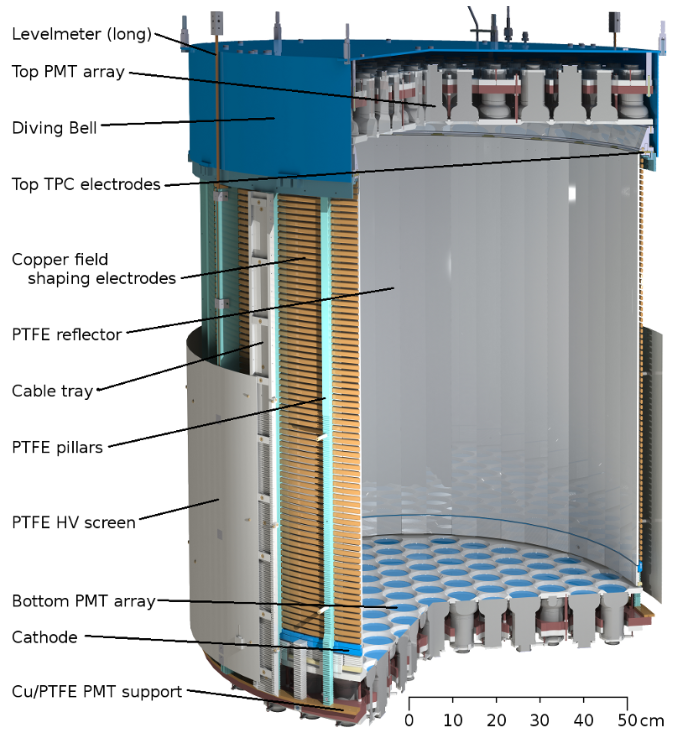
\includegraphics[width=0.8\textwidth]{XENON1TTPC}
\label{fig:xenon1t_tpc_tpc}
\end{figure}

There are five TPC electrodes that control the electric fields: the cathode, gate, anode, and top and bottom screening meshes.  They have
wired diameters of $\mathcal{O}(100)\ \mathrm{\mu m}$ and were designed to maximize S1 light collection.  The cathode is connected to a
PNC150000-1 NEG high voltage supply and pre-filling tests successfully reached voltages beyond -100 kV.  48
cm below the cathode is the bottom screening mesh (mentioned in \secref{subsec:xenon1t_pmts}).  The mesh is 12 mm above the bottom PMT
array and can be biased to reduce unwanted effects from the PMT and cathode E-fields.  The cathode and bottom screening mesh consist of
parallel wires and are gold-plated stainless steel, the latter of which increases the workfunction.  The gate rests just below the
liquid-gas interface and defines $z = 0$.  The anode is
situated 5 mm above the gate and is connected to a CAEN A1526P unit.  The fifth and final electrode is the top screening mesh 58 mm above
the anode and 11 mm below the top PMT array, and serves the same function is the same as the bottom mesh.  The top three electrodes are
made of stainless steel and are hex-etched.  Details for each electrode can be seen in \tabref{tab:xenon1t_tpc_electrodes} and
\figref{fig:xenon1t_tpc_efield} shows the simulated electric field for the settings during the first science run, Science Run 0.

\begin{table}
\centering
\begin{tabular}{cccccc}
\hline
Electrode & Type & Diamater & Material & Transparency & Position \\
\hline
Top screening & hex meshed & $178\ \mathrm{\mu m}$ & stainless steel & 96.5\% & 63 mm \\
Anode & hex meshed & $178\ \mathrm{\mu m}$ & stainless steel & 89.8\% & 5 mm \\
Gate & hex meshed & $127\ \mathrm{\mu m}$ & stainless steel & 92.7\% & 0 mm \\
Cathode & parallel wires & $216\ \mathrm{\mu m}$ & gold-plated stainless steel & 97.2\% & -969 mm \\
Bottom screening & parallel wires & $216\ \mathrm{\mu m}$ & gold-plated stainless steel & 97.2\% & -1017 mm \\
\hline
\end{tabular}
\caption{Properties for TPC electrodes.  The cathode and bottom screening mesh have high transparency to optimize S1 light collection and
are gold-plated to increase workfunction.}
\label{tab:xenon1t_tpc_electrodes}
\end{table}

\begin{figure}
\centering
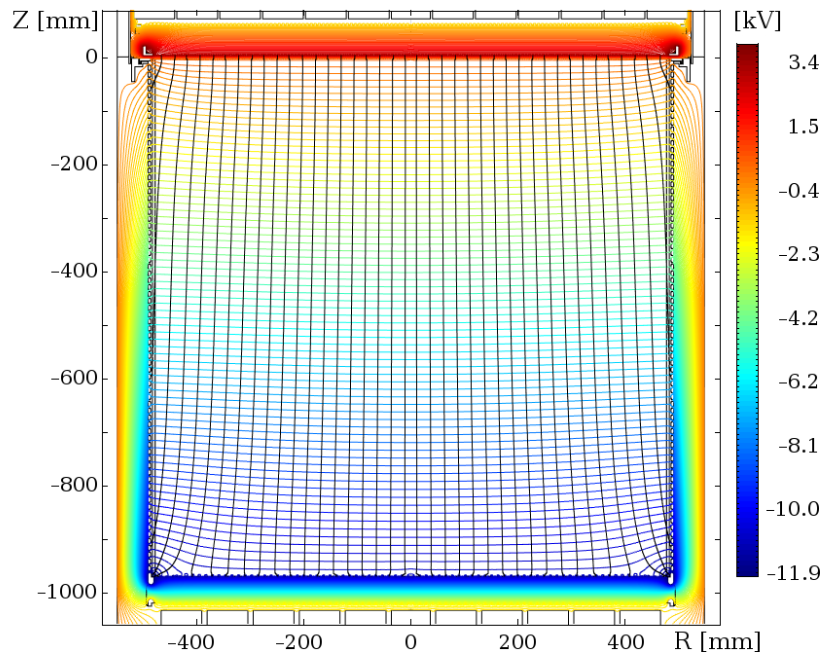
\includegraphics[width=0.8\textwidth]{ElectricField}
\caption{Finite element (COMSOL Multiphysics) simulation for E-field inside and around the TPC.  Field and equipotential lines are
shown.  The voltages for the cathode, gate, and anode are -12, 0, and 4 keV, respectively, or the settings for Science Run 0.  The field
is mostly uniform throughout the detector, minimizing possible biases that come from recombination, impurity attachment, etc.  Image
credit: \citeref{Aprile2017b}.}
\label{fig:xenon1t_tpc_efield}
\end{figure}

Four parallel-plate capacitors measure the liquid level.  They have a range of 10 mm with $30\ \mathrm{\mu s}$ precision and can be used
for observing tilts or raising (lowering) the TPC.  The liquid level's height is adjustable a gas-exhaust tube, and maintained with a
so-called ``diving bell" that uses controlled gas flow from purification to pressurize the GXe inside the TPC.  Two cylindrical levelmeters
with a range of 1360 mm extend from the bottom PMT array to above the diving bell and are used for filling and recovery.  Placed around the
field cage are cable trays that power and transfer signal from the PMTs.  They are made of PTFE and the cables are held
in place by PTFE spacers (\textbf{check if spacers is right word}).



\subsection{Cryogenics}
\label{subsec:xenon1t_cryo}
The TPC is stationed in the center of the water Cherenkov detector (\secref{subsec:xenon1t_water_shield}) and is encompassed by the inner
cryostat.  The cryostat
is stainless steel and electropolished to reduce radon emanation (\secref{}), since it is in direct contact with the xenon.  It is 1960 mm
tall by 1100 mm diamater and is metal-sealed
with Helicoflex.  Surrounding it is the 2490 mm tall by 1620 mm diamater outer cryostat.  It is also composed of stainless steel but
because there is no contact with xenon electropolishing is unncessary.  Materials were screened prior to construction for low-radioactivity
selection.  The two are thermally isolated by Torlon polyamide-imide spacers and
vacuum between them.  Heat loss is further mitigated to ${\sim} 75\ \mathrm{W}$ by aluminized mylar foil wrapped around the inner vessel.

A 10 m high stainless steel support structure was built inside the water tank.  Attached are three M20 rods that suspend the
cryostat.  They can be adjusted independently to tilt the cryostat, thereby changing the inclination of the LXe level with respect to the
TPC.  A chain secures the bottom of the outer vessel to the water tank floor to counteract buoyancy forces when the cryostat is empty.  A
double-walled pipe with inner and outer diameters 254 and 406 mm, respectively, connects with purification (\secref{subsec:xenon1t_pur}),
cooling,
pressurization for diving bell, and emergency recovery, and carries the PMT and auxiliary cables.  The voltage for the cathode is guided
in a separate pipe.  A schematic of the cryostat is shown

\begin{figure}
\centering
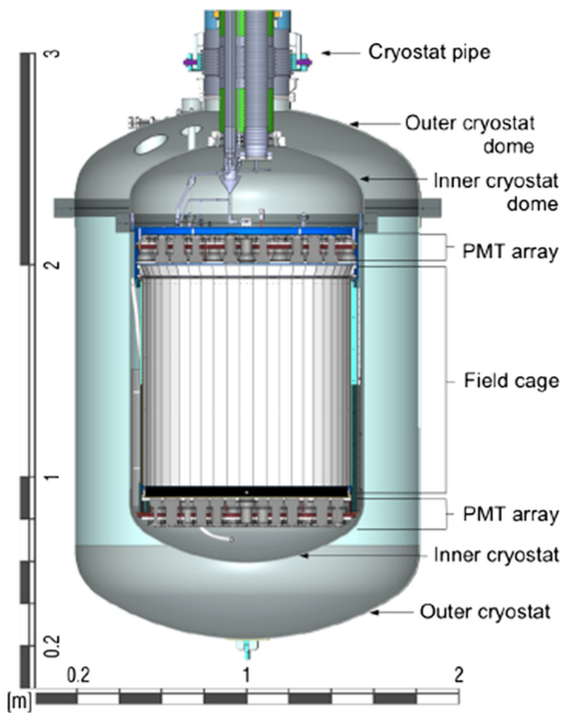
\includegraphics[width=0.8\textwidth]{CryostatDiagram}
\caption{Diagram of the cryostat.  Image credit: \citeref{Aprile2017c}.}
\label{fig:xenon1t_cryo_cryostat_diagram}
\end{figure}

A total of 3.5 tons of xenon is stored in the cryostat.  In addition to the 2.0 inside the TPC, the extra 1.5 is LXe between the
TPC and inner vessel or GXe above the liquid level.  The nominal LXe temperature is $T_{0} = -96^{\circ}\ \mathrm{C}$.  Gas near the top of
the cryostat is liquified by pulse-tube refrigerators (PTRs) into a funnel and flows back to the TPC through a designated pipe and
deposited in the inner vessel beneath the TPC.  Because
the PTRs are higher than the TPC the flow is guided by gravity.  \figref{fig:xenon1t_cryogenics_schmatic} shows the layout of the cryogenic
system.  The two PTRs occupy independent cooling towers and can each deliver ${\sim} 250\ \mathrm{W}$ of cooling power, and with
a total heat xenon heat load of ${\sim} 150\ \mathrm{W}$ only one needs to be active at any time.  The cooling towers along with much of the
GXe are located in the service building outside of the water tank  Each PTR connects to a copper cold finger
inside the inner cryostat so they can be removed without exposing the xenon to air.  A proportional-integral-derivative (PID) controller
monitors and adjusts the temperature of a resistive heater on the coldfinger to maintain stable pressure and temperature.

A third cooling tower uses liquid nitrogen ($\mathrm{LN_2}$) and is used in the case of an emergency if both PTRs are being serviced or the
heat load becomes too great from e.g. loss of power or insulation vacuum.  The $\mathrm{LN_2}$ flows from the $10 \mathrm{m^3}$ tank that
is used by ReStoX (\secref{subsec:xenon1t_restox}).  The cooling power can regulated by adjusting the $\mathrm{LN_2}$ evaporation rate.  In the event the PTRs
lose power the $\mathrm{LN_2}$ cooling tower must react immediately to prevent rising pressure that can be damaging to PMTs among other
things.  Sensors and controllers monitoring such a power loss are powered with uninterruptible power supplies (UPSs) to ensure a successful
transition and operation of $\mathrm{LN_2}$.

\begin{figure}
\centering
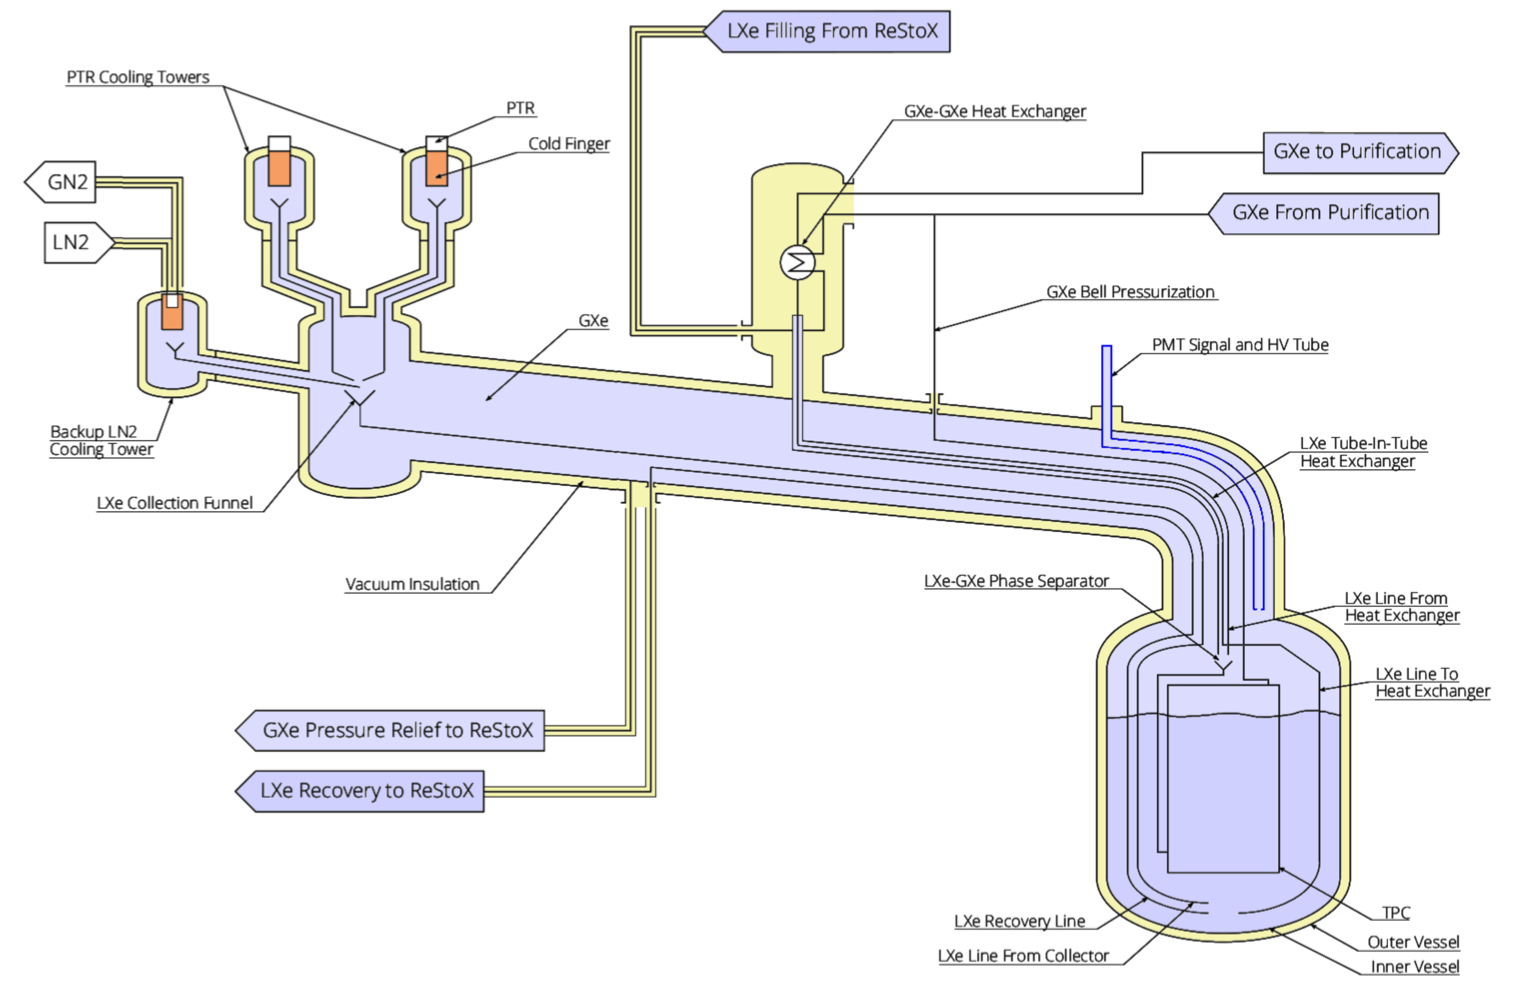
\includegraphics[width=\textwidth]{CryostatSchematic}
\caption{Layout of the cryogenic system.  Three cooling towers - two with PTRs and one backup $\mathrm{LN_2}$ - liquify GXe to return to
the TPC.  LXe is carried from the bottom of the cryostat to the purification system (\secref{subsec:xenon1t_pur}) through a heat exchanger
system, where
returning xenon is inserted into the bottom of the TPC with excess gas diffusing into the GXe.  A fraction of purified GXe is extracted
before the heat exchanger and used to maintain pressure inside the diving bell.  ReStoX (\secref{subsec:xenon1t_restox}) connections are
also shown.  Image credit: \citeref{Aprile2017b}.}
\label{fig:xenon1t_cryogenics_schematic}
\end{figure}

Connections to purification and ReStoX are shown in \figref{fig:xenon1t_cryogenics_schematic}.  The LXe carried to the purification system
passes through a heat exchanger system discussed in \secref{subsec:xenon1t_pur}.  This is not the case for recuperation since the xenon
does not need to be gaseous.

LXe from the beneath the TPC (near liquid line from PTRs) is removed for purification.  Once the xenon removed from the LXe it passes
through a two-phase heat exchanger system.  The function of the heat exchanger is for GXe (returning to the TPC) and LXe (leaving) to
exchange thermal energy.  This way the returning xenon is cooled before it reaches the TPC, and likewise removed xenon is heated before
the purification.  The first step of the system is the ``tube-in-tube" component where two concentric tubes carrying LXe (GXe) away from
(towards)
the TPC.  The second component is a plate heat exchanger and is closer to the purification system (i.e. returning xenon passes through
before tube-in-tube).

We can define the heat exchange
efficiency $\epsilon$ as the fraction of heat necessary for temperature change and vaporization that stays outside of the system.  A higher
efficiency results in greater thermal energy transferred between the GXe and LXe and thus decreases the heat load on the system.  This is
because instead of GXe entering the cryostat at roughly
room temperature, it returns at approximately that of LXe, with much of it having condensed to LXe, putting less stress on the
PTRs.  An essential ingredient of the heat transfer is the latent heat, which comprises ${\sim} 80\%$ of the total exchange.  The difference
in vaporization temperature of the outgoing xenon and condensation temperature of incoming xenon is given by

\begin{equation}
\Delta T_{\mathrm{ph}} = T_{\mathrm{gl}} (P_i) - T_{\mathrm{gl}} (P_o)
\label{eq:xenon1t_cryo_latent}
\end{equation}

where $T_{\mathrm{gl}} (P)$ is the temperature of the gas-liquid phase transition that depends on pressure, and $P_i$ and $P_o$ are the
pressures of the incoming and outgoing xenon, respectively.  Because the conditions of the dynamical gas flow
(\secref{subsec:xenon1t_pur}) cause $P_i > P_o$, $\Delta T_{\mathrm{ph}} > 0$, making it effective at heat transfer
(\citeref{Aprile2012b}).  A study with the Demonstrator - the
experiment used to for research and development for XENON1T - showed a heat exchange efficiency of
two heat exchangers in series of $\geq 96\%$ (\citeref{Aprile2012b}).  Following the parallel-plate exchanger a heater provides additional
thermal energy to the xenon moving towards the purification system.  The different systems that handle the xenon can be seen in
\figref{fig:xenon1t_cryo_overview}.

\begin{figure}
\centering
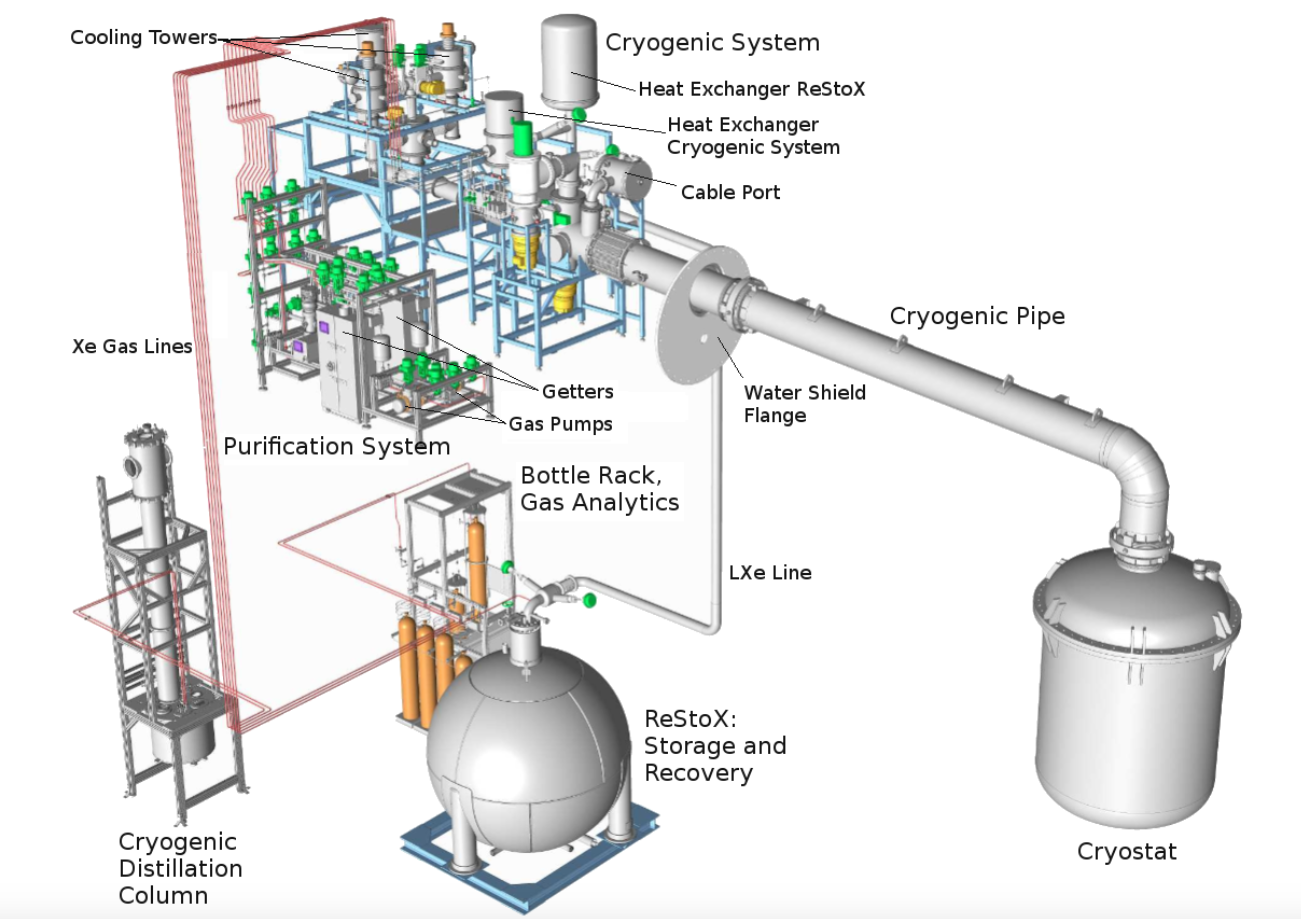
\includegraphics[width=\textwidth]{CryoOverview}
\caption{The various systems that handle xenon in the experiment: cryostat, cryogenics, purification, cryogenic distillation column,
ReStoX, bottle racks, and gas analytics station.  The water shield flange defines the region between the service building and the water
Cherenkov detector.  Image credit: \citeref{Aprile2017b}.}
\label{fig:xenon1t_cryo_overview}
\end{figure}



\subsection{Purification}
\label{subsec:xenon1t_pur}
Contamination in LXe can present a number of problems.  As mentioned in \secref{subsec:tpcs_working_principle} electronegative
impurities (e.g. O$_2$, H$_2$O, N$_2$O, etc.) will attach to drifting $e^-$, reducing the number that reach
the liquid surface and thus the S2.

Impurities will also attenuate scintillation, which pushes our energy threshold up as fainter signals become harder to detect.  This is
described by

\begin{equation}
I(x) = I_0 e^{-x / \lambda_{\mathrm{att}}}
\label{eq:xenon1t_pur_atten}
\end{equation}

where $I_0$ is initial number of photons, $I(x)$ is the number after traveling a distance $x$, and $\lambda_{\mathrm{att}}$ is the
attenuation length.  $\lambda_{\mathrm{att}}$ is dependent on the absorption and scatter lengths, $\lambda_{\mathrm{abs}}$ and
$\lambda_{\mathrm{scat}}$.  The absorption length describes the true loss of photons while the scatter refers to photons that elastically
scatter without energy loss.  The attenuation length can then be written
$1 / \lambda_{\mathrm{att}} = 1 / \lambda_{\mathrm{abs}} + 1 / \lambda_{\mathrm{scat}}$.  \figref{fig:xenon1t_pur_absorption_spectra} shows
the Xe scintillation spectrum along with the absorption coefficients for \otwo and \htwoo vapor at concentrations of 1 ppm.  We can see
there is large overlap at lower wavelengths - especially for H$_2$O - and that observations under these circumstances would lead to an
incorrect measurement of the scintillation spectrum.  In addition to electronegative there are intrinsic
impurities including Kr and Rn but these are discussed in \secref{subsec:xenon1t_kr_dist}.

\begin{figure}
\centering
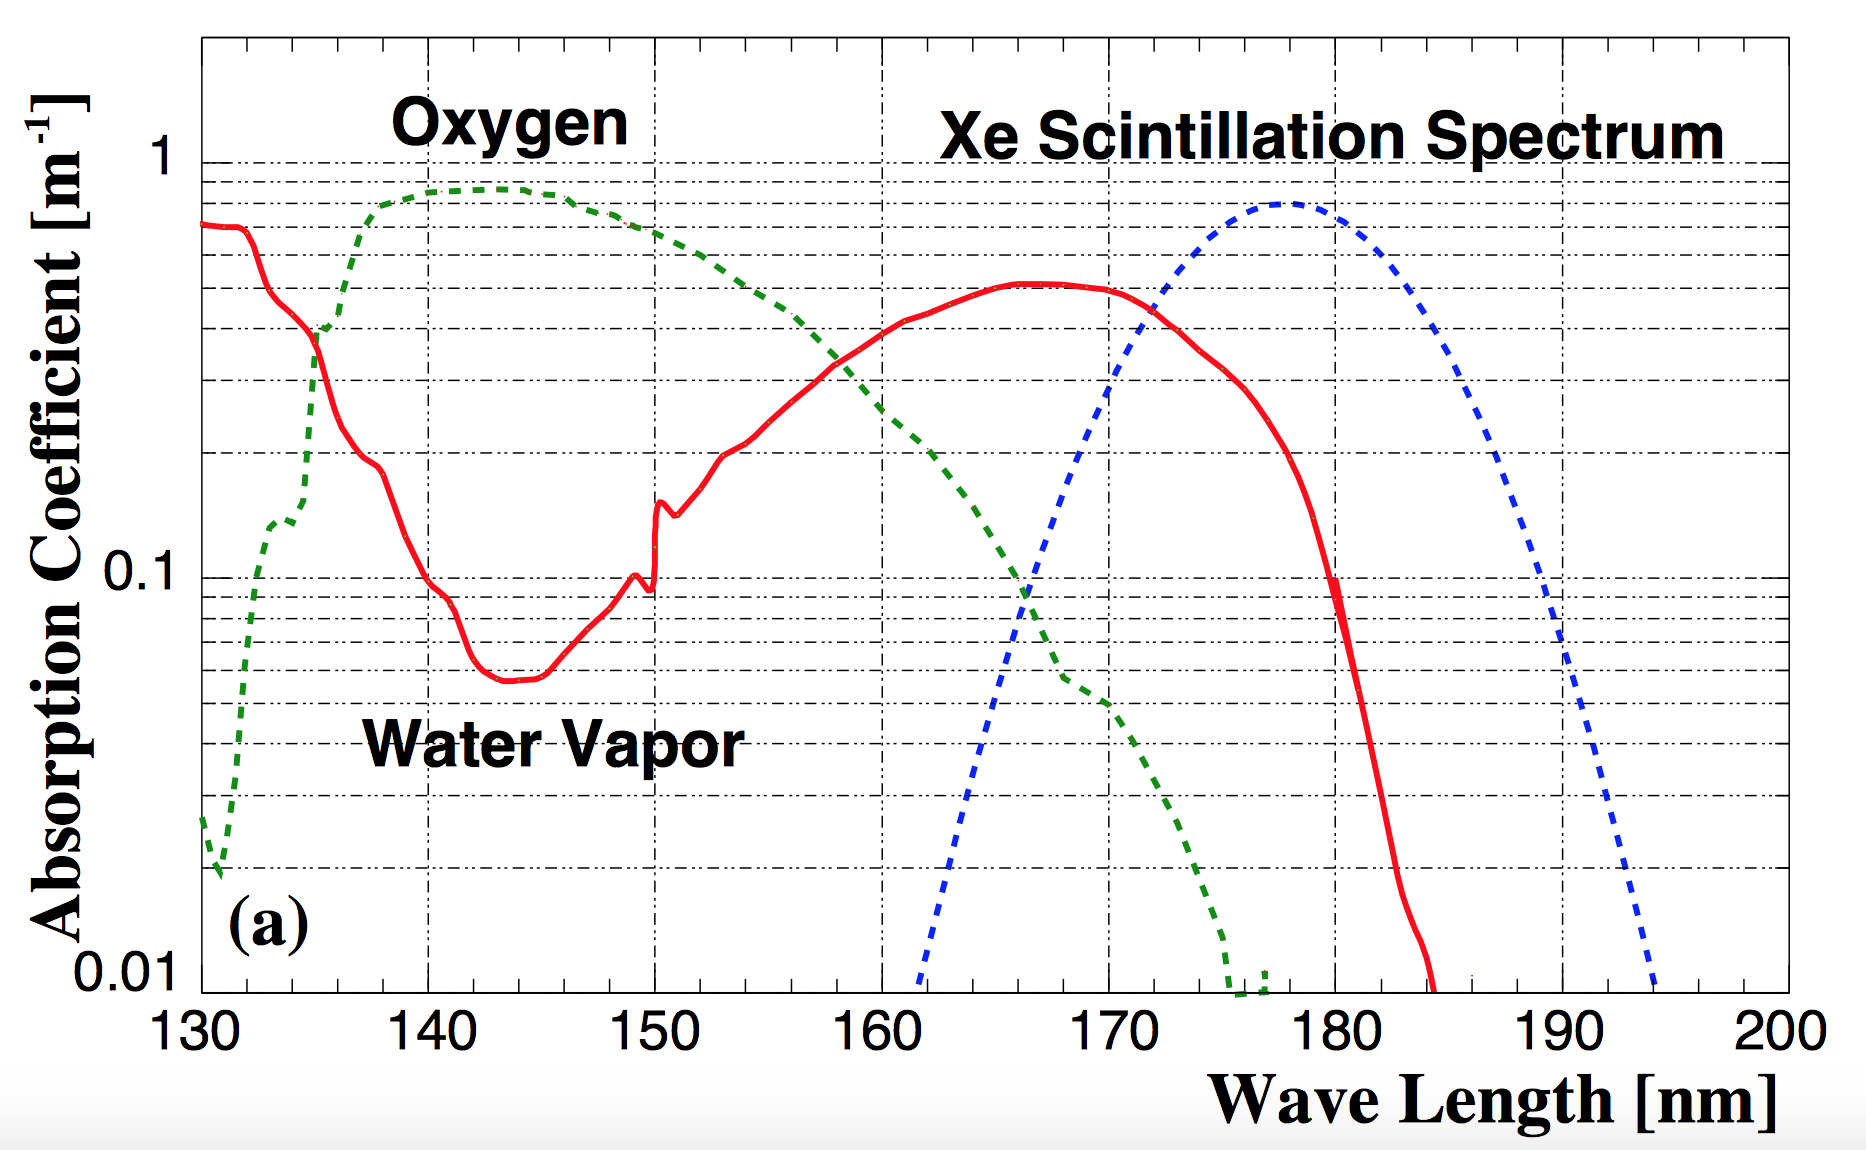
\includegraphics[width=0.8\textwidth]{AbsorptionSpectra}
\caption{Xe scintillation spectrum along with absorption coefficients for oxygen and water vapor present at 1 ppm.  \otwo has a maximum
value of overlap
with Xe of ${\sim} 0.1$ around 166 nm.  \htwoo covers a larger range of xenon's spectrum and has a much more significant impact, with a
maximum value of $> 0.4$ at approximately 172 nm and ${\sim} 0.2$ at 178 nm.  Image credit: \citeref{Ozone2005}.}
\label{fig:xenon1t_pur_absorption_spectra}
\end{figure}

\begin{figure}
\centering
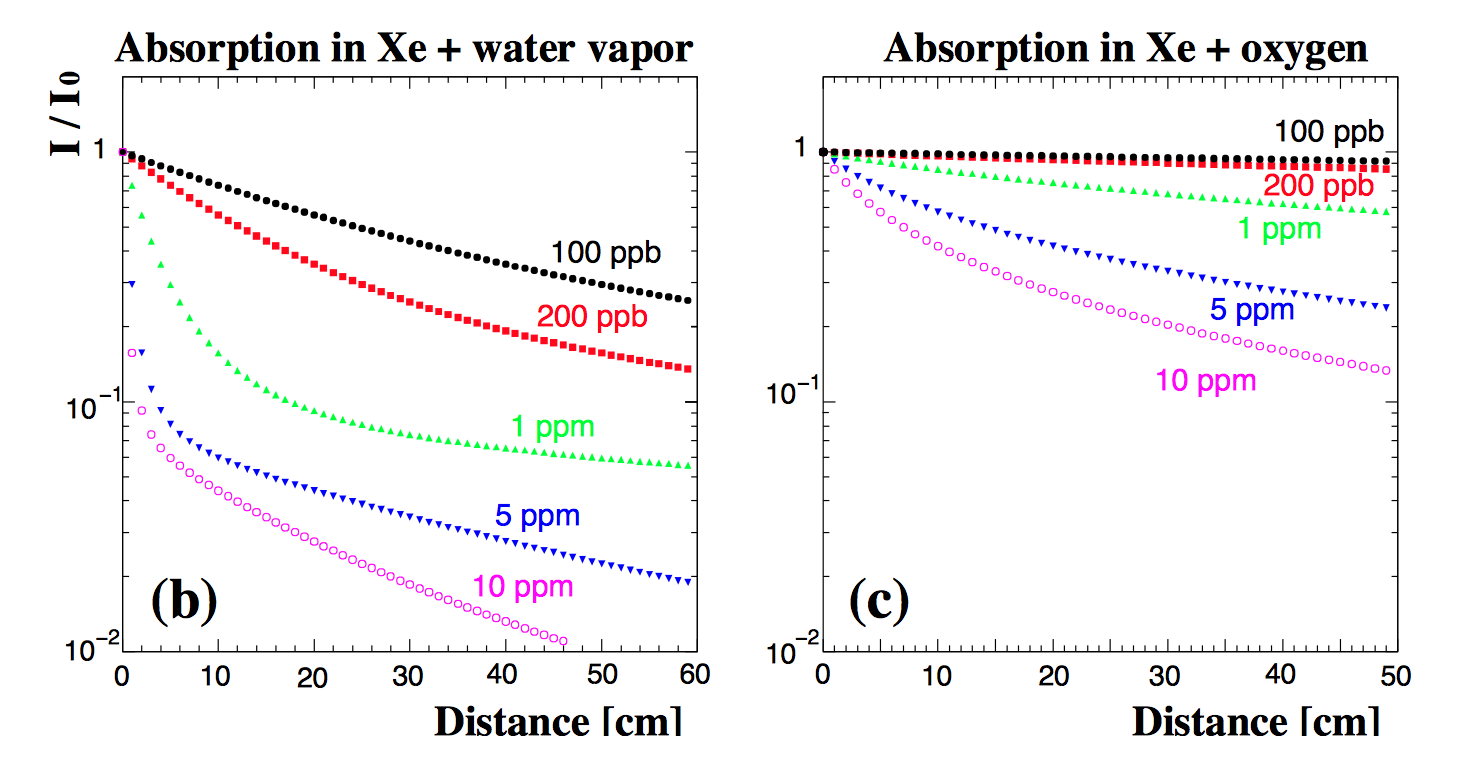
\includegraphics[width=\textwidth]{AbsorptionWithDistance}
\label{fig:xenon1t_pur_absorp_dist}
\end{figure}

Electronegative impurities come primarily from outgassing of detector materials.  They have different \electron attachment rates (see
\figref{fig:attachment_rate} for examples) so are measured in O$_2$-equivalent - that is, the analogous concentration of oxygen if it
were the only contaminant.  For LXe experiments the necessary concentration is $\mathcal{O}(10^{-9})$ parts per billion (ppb) or less.

In addition
to the GXe from the TPC (after passing through heat exchanger and heater as described in \secref{subsec:xenon1t_cryo}), connections are
made between
each of the cooling towers and the purification system.  Because impurities are lighter than xenon we can anticipate them having a larger
presence in the gas.  While the GXe impurity concentration has no direct effect on \electron loss, impurities should migrate between the
LXe and GXe.  Purifying the GXe then should largely reduce the impurities that pass into the liquid.

Xenon from ReStoX  (\secref{subsec:xenon1t_restox}) and bottles are also connected to the purification system.  A separate heat exchanger
sits between ReStoX and purification but is less effective when xenon is not incoming and outgoing (not during detector filling).  In
addition to cleaning the Xe as it is transfered to the from RestoX to the cryostat, the purification system connects ReStoX to the Kr
distillation column (\secref{subsec:xenon1t_kr_dist}).  The column returns the xenon after distillation to purification.  All systems that
feed into the purification system do so before the getters and are available as outputs as well.  A small tube between the purification
and cryostat before the heat exchanger siphons GXe to the TPC bell to maintain pressure, and is regulated by a flow controller.  The
numerous connections makes the purification system a hub for transferring xenon between systems.

\begin{figure}
\centering
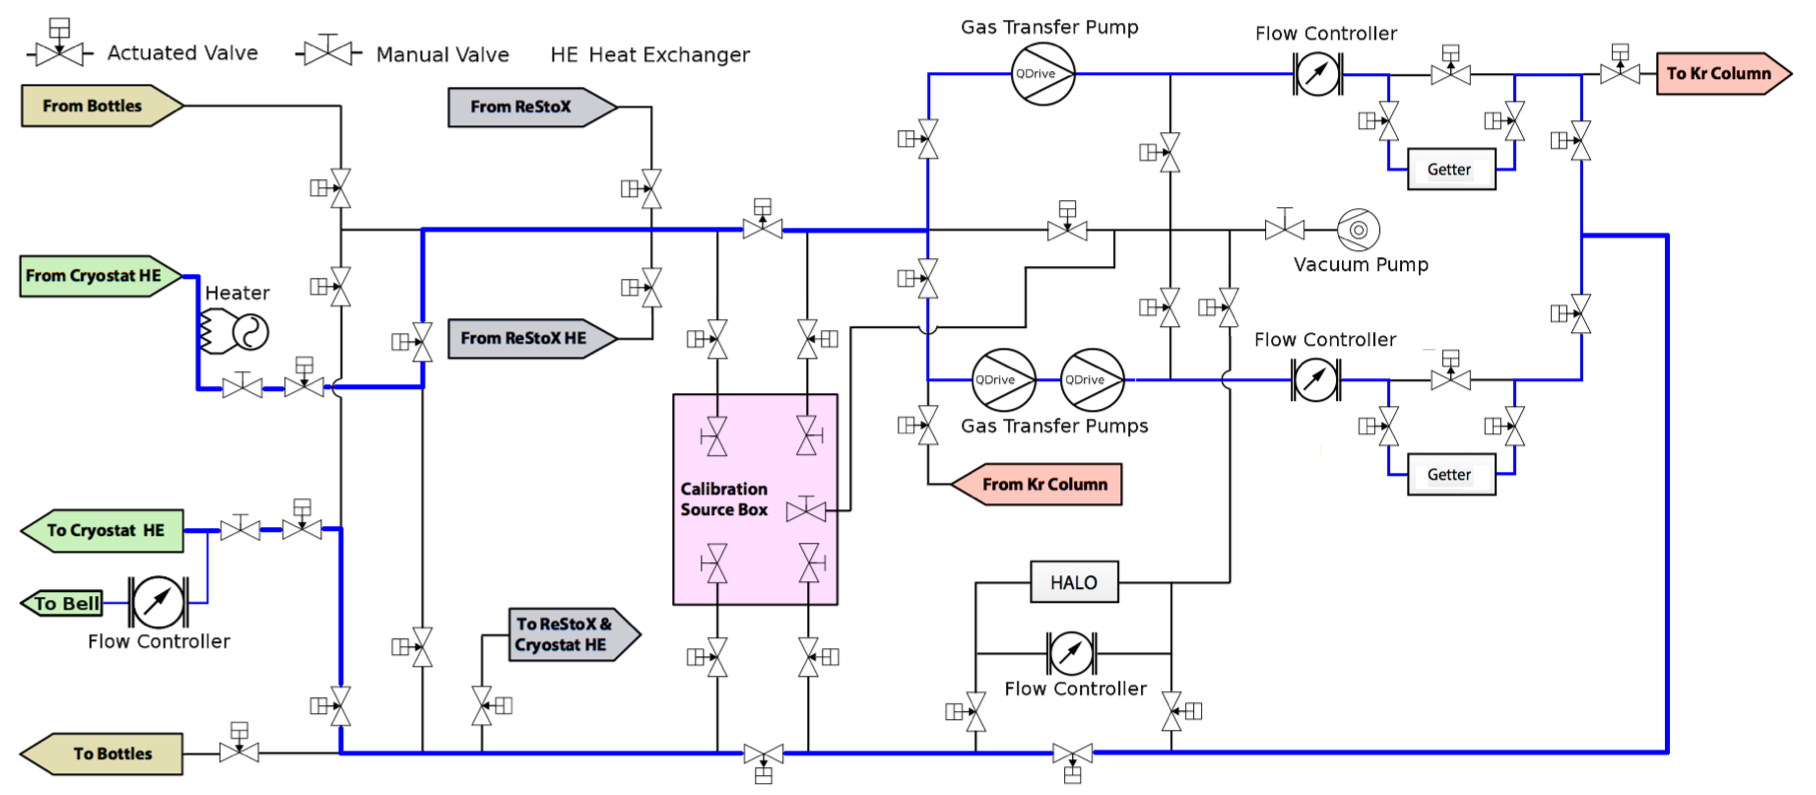
\includegraphics[width=\textwidth]{PurificationLayout}
\caption{Image credit: \citeref{Aprile2017b}.}
\label{fig:xenon1t_pur_schematic}
\end{figure}

The purification system consists of two redundant purification loops, each of which can operate independently of the other.  The flow
is driven by CHART QDrives, with one on one loop and two on the other.  They were chosen for their high-capacity and hermetically sealed
pump volume, the latter of which was not true with KNF pumps that were used in XENON100 (\textbf{check this}).  This is important because
exposure to air could cause a significant drop in purity, and has occurred in the past with KNFs.  They are
magnetically-resonant and operate via a compression space with oscillating externally-driven pistons.  Motors, valves, and pistons are
not lubricated, making it an excellent choice for high-purity.  Unfortunately QDrives emanate \ce{^{222}Rn} can require frequent
maintenance if operated at too great a voltage (for larger flow).  For the former \ce{Rn} emanation measurements were made prior to
installation with the lowest being chosen.  For the latter they are operated at safe conditions and since the beginning of Science Run 0
no issues have arisen.  It turns out the limiting factor on our circulation speed is not a result of the pumps but the pressure difference
from tubes leading to the system caused by too small a radius.  With the upgrade to XENONnT these will be replaced with larger-radii.  One
QDrive is installed in one loop and two in the other.

The flow of the GXe is maintained by two MKA 1579A mass-flow controllers - one on either branch.  The assumption before the experiment went
online was these would limit the speed when necessary, but because we did not achieve our goal these have minimal impact.  Still, they can
be used for further restriction.  The xenon then passes through SAES PS4-MT50-R high-temperature rare-gas purifiers, or getters.  They
use heated ($400^{\circ}\ \mathrm{C}$) zirconium to form unbreakable bonds with carbide, nitride, and oxide, lowering the impurity content
to < 1 ppb.  A bypass valve allows the xenon to pass un-purified in the event that the it does not need to be cleaned.

A Tiger Optics HALO+ H$_2$O monitor measures the water content in the purified GXe to track the purification efficiency.  It can measure
concentrations down to 400 ppt.  As with the getters, it can be bypassed.  The Xe is then forwarded to the cryostat, bell, ReStoX, or
bottles (Kr column occurs after the purification loops before the HALO).

The components of the system are electropolished and able to be baked up to ${\sim} 120^{\circ}\ \mathrm{C}$ for decreased outgassing during
operation.  The purification system has a number of valves that allow the versatility described in this section.  The majority are pneumatic and can
be operated remotely with the slow control system.  The remainder are manual valves situated in select locations: to and from the cryostat,
inside the calibration box, and before the vacuum pump, which can be used to evacuate individual sections or all of the system.  These are
in place as a precaution against accidental openings of the actuated valves that could produce problems.


\subsection{ReStoX}
\label{subsec:xenon1t_restox}
The Recovery and Storage system for XENON1T (ReStoX) hosts xenon not in use by other systems.  It is located roughly 7 on the ground floor of the
service building.  With a volume of 4.95 m$^{3}$
(diameter of 2.1 m), wall thickness of 28 mm, and ability to withstand pressures up to 73 bar, it can support as much as 7.6 tons of xenon
as a gas, liquid, or super-critical fluid.  It is constructed from stainless steel and insulated with vacuum from an outer sphere, where
thermal conductance is minimized with superinsulation and limited contact to an external heat load of ${\sim}50\ \mathrm{W}$.  To limit
impurity contamination while the Xe is in ReStoX the vessel and valves are metal sealed and electropolished.

The xenon is cooled by LN$_2$ that is housed in a 10 m$^3$ dewar adjacent to the service building.  This is done in part with 16 LN$_2$
lines that are welded to the inner vessel's outer surface.  To prevent over-cooling 16 stainless steel fins inside increase heat
exchanging.  A condenser and heater in the middle are used when the xenon is stored as a liquid, which is the nominal state of
operations.  The heater ensures solid xenon does not block pipes so Xe can transfer freely with other systems.  The total cooling power is
spread over 4.3 m$^2$ of copper with magnitude of over $>3\ \mathrm{kW}$.

\begin{figure}
\centering
\includegraphics[width=0.8\textwidth]{ReStoX}
\caption{Image credit: \citeref{Aprile2017b}.}
\label{fig:xenon1t_restox_pic}
\end{figure}

Previous LXe experiments would fill the detectors by condensing the GXe from storage.  Similarly, recovery was done by allowing the LXe
in the cryostat to evaporate.  While this was achievable for detectors with $\mathcal{O}(100)\ \mathrm{kg}$ of xenon, doing so
(\textbf{maybe it is just for filling, check}) for XENON1T would require approximately two months, and fast recovery in the event of an
emergency would not be possible.  This is solved through the purification system, which as mentioned in \secref{subsec:xenon1t_pur} can
pump xenon between systems (\textbf{check with someone about how xenon is recovered}).



\subsection{Krypton Distillation}
\label{subsec:xenon1t_kr_dist}
Commercial high-purity xenon generally has \ce{Kr} concentrations from 1 ppm down to 10 ppb.  This is not clean enough for LXe dark matter
detectors so additional distillation is necessary.  The reason for restricting the
krypton content is \ce{^{85}Kr}, which undergoes \betadecay with an end-point energy of 687 keV and a half-life of 10.76 years.  With
an expected fraction $\mathrm{^{85}Kr / ^{nat}Kr = 2 \times 10^{-11}}$ the required \ce{^{nat}Kr}/Xe concentration for its background to be
less than radon is $< 200\ \mathrm{ppq}$.  Details of the \ce{^{85}Kr} background can be found in \secref{sec:backgrounds}.

To achieve the intended purity we use a Kr distillation column, seen in \figref{fig:xenon1t_kr_dist_column}.  The column is has a total
height of 5.5 m and is kept in an insulation vessel at $10^{-5}\ \mathrm{mbar}$ to minimize thermal losses (citeref{Aprile2016b}).  GXe
that is passed to the column enters through a heat exchanger and is
liquified by the input condenser.  The input condenser uses a cryo-cooler (Leybold CP-50) at $-98^{\circ}\ \mathrm{C}$ and maximal power
of 100 W.  Next it passes to the package tube, built with 2.8 m of structured stainless steel package material (Sulzer EX) 45 cm in
diamater that has feeding ports for both liquid and gaseous xenon.  At the top of the tube is a second cryo-cooler (Leybold CP-140T)
operating at $-98^{\circ}\ \mathrm{C}$ with 200 W.  Liquified xenon will fall towards the bottom, where it is stored and heated by a
reboiler with a maximum of 300 W.  The Kr, with a lower atomic mass will drift towards the top of the column but will not liquify as its
boiling point is lower than $-98^{\circ}\ \mathrm{C}$.  Siphoning the xenon at the top then removes Kr at a much higher concentration than
present in the inlet GXe.  Purer Xe at the bottom is extracted where it passes through the heat exchanged before returning to the
purification system or ReStoX (\textbf{check this}).

\begin{figure}
\centering
\includegraphics[width=0.6\textwidth]{KrColumn}
\caption{Image credit: \citeref{Aprile2017b}.}
\label{fig:xeno1t_kr_dist_column}
\end{figure}

After installed at LNGS the reduction of \ce{^{nat}Kr}/Xe was found to be $6.4_{-1.4}^{+1.9} \times 10^{5}$
(\citeref{Aprile2016b}).  Inlet flows have been shown to be stable up to 18 SLPM, but running all ReStoX xenon through distillation before
cryostat filling would take ${\sim}3$ weeks.  For this reason an ``online" removal system was used, where the xenon was distilled during
science run data taking.  Over 70 days 7\% of xenon passing through purification was diverted to the column and a total 0.07\% was
removed.  An initial \ce{^{nat}Kr}/Xe concentration of 60 ppb was decreased to $360 \pm 60\ \mathrm{ppq}$, the lowest ever realized in a
LXe dark matter experiment.  Such low concentrations are measured by a rare gas mass spectrometer (RGMS) that uses cryogenic gas
chromotography to separate the Kr from Xe, followed by a mass spectrometer for Kr measurement (\citeref{Lindemann2014}).

A second low-energy background comes from the \ce{^{222}Rn} decay chain.  While the distillation column was built and intended for Kr,
it was shown to work in a single stage distillation (\citeref{Bruenner2017}) and subsequently XENON100
(\citeref{Aprile2017d}).  It operates using the reverse principle, i.e. Rn-enriched xenon is coalesces near the bottom of the column.



\subsection{Water Shield}
\label{subsec:xenon1t_water_shield}
Limiting radiation from outside the experiment is essential to a dark matter search.  An active water Cherenkov detector encompasses the
cryostat, spanning 9.6 m in diamater and 10.2 m high.  It is filled with deionized water, which can fill the detector at up to
$2.2\ \mathrm{m^{3}/hour}$.  The tank shields the cryostat from neutrons and \gammarays that originate underground (from e.g. rocks),
decreasing the event rate by orders of magnitude.  It can identify muons as well as muon-induced neutrons by detecting showers initiating
outside the water tank.  If an event in the TPC coincides with one in the water tank it will usually be excluded incase the two are
related, acting as a muon veto.  The flux of muons at LNGS is $3.31 \pm 0.03 \times 10^{-8}\ \mathrm{cm^2\ s^{-1}}$ with average energy
${\sim}270\ \mathrm{GeV}$ (\citeref{Aprile2017b}).

84 Hamamatsu R5912ASSY PMTs are placed in five rings along the inner wall of the tank, each 2.5 m apart in height.  The lowest
($z = 0\ \mathrm{m}$) and highest ($z = 10\ \mathrm{m}$) each contain 24, while the three between them have 12.  The quantum efficiency
is ${\sim}30\%$ between 300-600 nm.  To increase the chance of photon detection the inner wall is coated with foil (3M DF2000MA) that has
nearly 100\% reflectivity at $> 400\ \mathrm{nm}$, (\citeref{2017Geis}).  However, ${\sim}90\%$ of light is absorbed for $<370 \mathrm{nm}$
and 3-7.5\% from $250 < \geq \lambda \geq 370\ \mathrm{nm}$ is wavelength shifted to more favorable values for the PMTs.

\begin{figure}
\centering
\includegraphics[width=\textwidth]{MuonVetoPhoto}
\label{fig:xenon1t_water_shield_photo}
\end{figure}

\begin{figure}
\centering
\includegraphics[width=\textwidth]{InsideWaterTank}
\label{fig:xenon1t_water_shield_interior}
\end{figure}



\subsection{Calibrations}
\label{subsec:xenon1t_calibrations}
Calibrations are used for a host of purposes including understanding energy resolution, light collection efficiency, electron lifetime,
$g_1$, $g_2$, electronic and nuclear recoil bands, and many more.  Depending on the source they can be performed inside the TPC (internal) or
outside (external).  Here I cover the different calibrations and the purposes they serve; additional details and results are in
\secref{sec:det_char}.

\begin{figure}
\centering
\includegraphics[width=\textwidth]{Panoramic}
\label{fig:xenon1t_panoramic}
\end{figure}

\subsubsection{Internal}
\label{subsubsec:xenon1t_calibrations_internal}
Internal calibrations allow us to describe how our detector observes events throughout the entire TPC.  This is preferabel to external
calibrations, where only part is used.  The calibration source box is installed in the purification system (pink region in
\figref{fig:xenon1t_pur_schematic}) and contains valves opening to the GXe both before and after the getters.  When the valves are opened,
the source will flow into the GXe stream and into the cryostat and mix with the xenon.  We therefore only use sources that do not introduce
electronegative impurities.  The source will quickly spread itself throughout the entirety of the xenon, giving a uniform distribution,
and allowing us to improve our understanding of how variation in observables relates to position.

\kryptonmeta has two monoenergetic decays at 32.15 ($t_{1/2} = 1.83\ \mathrm{h}$) and 9.4 keV ($t_{1/2} = 154.4\ \mathrm{ns}$).  The short
half-lives coupled with its final decay product, \ce{^{83}Kr} being stable makes it a great choice to calibrate the light collection
efficiency (LCE) and measure the electron lifetime.

\radoncal is used to calibrate the ER band as \ce{^{212}Pb} - one of its daughters, is a $\beta$-emitter with endpoint energy
569.91 keV.  There are additional $\alpha$, $\beta$, and $\gamma$ emissions throughout the chain that can be used for additional studies,
including measuring the electron lifetime with the \ce{^{212}Bi} $\alpha$-decay (6.207 MeV).  The longest half-life in the chain is
\ce{^{212}Pb} with $t_{1/2} = 10.6\ \mathrm{h}$ (next longest is \ce{^{212}Bi} with $t_{1/2} = 1.00\ \mathrm{h}$), which allows DM data
to resume within several days.

Tritiated methane ($\mathrm{C H_3 T}$) is a very attractive candidate because of it's low-energy $\beta$-emission.  With a 18.6 keV
endpoint energy, it is an ideal candidate for calibrating the low-energy (cs1 < 100 pe, \textbf{check this}) ER band, and even measuring
the light and charge yield in a relatively unexplored but important region.  This was originally done by LUX (\citeref{LUX2016}) and
subsequently performed with XENON100 (\citeref{Aprile2017e}).  However, with a half-life of $t_{1/2} = 12.3\ \mathrm{y}$ it must be
removed completely by the getters to avoid introducing a new background.  This is further complicated by a suspicion that
$\mathrm{C H_3 T}$ adheres to the cryostat, prohibiting total removal.  For this reason a $\mathrm{C H_3 T}$ calibration has not yet been
conducted in XENON1T.

PMT gains are calibrated using blue LEDs at low light levels.  Unlike the previous sources this calibration is done using cables that are
carried from the data acquisition (\secref{subsec:xenon1t_daq}) into the TPC.  They are fixed at various heights and angles and flash
at periodic intervals.  The result is an SPE spectrum as shown in \figref{fig:xenon1t_pmt_spe}.

\begin{figure}
\centering
\includegraphics[width=\textwidth]{WaterTankInside}
\label{fig:water_tank_inside}
\end{figure}



\subsubsection{External}
\label{subsubsec:xenon1t_calibrations_external}
External calibrations are performed with a source outside the cryostat.  In XENON100 this was done by inserting a source inside the lead
shielding; however, the water tank in XENON1T makes this a more complicated task.  The resolution was the installation of two ``I-belts"
along the height of the detector and one ``U-belt" that also extends underneath, as shown in \figref{fig:xenon1t_calibration_belts}.  These
allow the sources to be lowered from the roof of the tank, as well as calibrate from different locations, so long as they are on the
belts.  They are removed during dark matter data taking.

\begin{figure}
\centering
\includegraphics[width=0.8\textwidth]{TPCCalibrations}
\caption{Image credit: \citeref{Aprile2017b}.}
\label{fig:xenon1t_calibrations_belts}
\end{figure}

External $\gamma$ sources include \ce{^{137}Cs}, with an energy of 661.7 keV, and \ce{^{228}Th}, with a number of energies between 511 keV
and 2.614 MeV.  These are installed in W-collimators that restrict the \gammarays to a cone of $40^{\circ}$.  Additionally, \ce{^{60}Co}
in the cryostat flanges with 1.173 and 1.333 MeV lines can also be used.

Nuclear recoil sources \ambe and a deuterium-deuterium (DD) neutron generator (NG) are also placed outside the TPC.  It is also deployed in a
W-collimator and emits MeV neutrons.  Details are discussed in \secref{subsubsec:er_nr_calibrations_parameter_determ_nr}.



\subsection{Data Acquisition}
\label{subsec:xenon1t_daq}
The data acquisition (DAQ) is in a temperature-controlled room on the second floor of the service building.  It can record the TPC and
muon veto PMTs either independently or simultaneously.  The signals from the TPC first pass through Phillips Scientific 776 amplifiers
where they undergo 10-fold amplitude increase.  They, along with the muon veto signals, are then digitized via 100 MHz CAEN V1724 flash
ADC boards (32 in total) that have 40 MHz bandwith, 14 bit resolution, and 2.25 V or 0.5 V, respectively.  A single independent clock
connects to each ADC to ensure they are properly aligned and a 0.1 Hz synchronization signal is passed from a custom-developed GPS-synched
module.

The TPC DAQ reads every pulse $> 0.3\ \mathrm{PE}$ from each PMT independently and regardless of any signal from other
channels.  The read-outs of the ADC boards are passed to six computers at up to $300\ \mathrm{MB\ s^{-1}}$ (${\sim}100\ \mathrm{Hz}$) and
are stored - along with relevant information such as time and channel - in a MongoDB database.  The sum of the bottom PMTs along with veto
and busy information is constantly read by a separate computer to determine the deadtime.  The DAQ continuously monitors data quality
parameters such as baseline, trigger, and noise.

A software eventbuilder on three server-grade machines decides if an interaction has occurred in real-time by examining the
time-clustering of PMT signals, and opts whether or not to trigger.  Metadata from the trigger decision is recorded and can be monitored
online to check performance or offline for analysis.  At larger than 200 PE (${\sim}7\ e^-$) the trigger efficiency is $> 99\%$.  The muon
veto uses a simple coincidence trigger that is directed by a CAEN V1495 VME unit.

Two 10 Gbps fibers transfer the raw data to buffer-storage at LNGS for temporarily housing.  The raw data is then moved to the US Open
Science Grid and European Grid Infrastructure for processing and backed up in Stockholm.  \figref{fig:xenon1t_daq_schematic} shows an
overview of the DAQ system.

\begin{figure}
\centering
\includegraphics[width=\textwidth]{DAQ}
\label{fig:xenon1t_daq_schematic}
\end{figure}



\section{Backgrounds}
\label{sec:backgrounds}
To reach the desired sensitivity it is crucial to lower our backgrounds as much as possible, and just as importantly, understand
them.  Our backgrounds mainly come from the detector materials, radioactive isotopes distributed inside the xenon, and space.

\subsection{Detector Materials}
\label{subsec:backgrounds_detector_materials}
As mentioned in \secref{subsec:xenon1t_pmts} and \secref{subsec:xenon1t_cryo} detector materials were screened before purchasing to ensure
those with the lowest radioactivity were chosen.  The high self-shielding power of LXe prevents the radiation from penetrating far into
the detector, stopping the majority within several cm.  Still, it is important to understand our background for a number of reasons.  The
first is we want to maximize our FV.  But because including these events can have a negative effect on our sensitivity, we need to know
what a safe distance from the top, bottom, and wall are.  The second is once we choose our FV it is important to have a reliable estimate
of the number of events that will ``leak" into our FV, known as ``leakage events".  Failing to have an accurate prediction can result in
a cost in sensitivity.  A third reason is these events can play a significant role in characterizing the detector.

The primary isotopes from materials that play a role in our background are \ce{^{40}K}, \ce{^{60}Co}, \ce{^{235}U}, and the decay chains
of and \ce{^{238}U}, \ce{^{232}Th}, \ce{^{228}Th}, and \ce{^{226}Ra}.  In fact, although \ce{^{226}Ra} and \ce{^{228}Th} are part of the
\ce{^{238}U} and \ce{^{232}Th} chains, respectively, the measured disequilibrium prompts us to separate them as
$\mathrm{^{238}U} \rightarrow \mathrm{^{230}Th}$ and $\mathrm{^{226}Ra} \rightarrow \mathrm{^{206}Pb}$ for \ce{^{238}U}, and
$\mathrm{^{232}Th} \rightarrow \mathrm{^{228}Ac}$ and $\mathrm{^{228}Th} \rightarrow \mathrm{^{208}Pb}$ for \ce{^{232}Th}.  The full
\ce{^{238}U} and \ce{^{232}Th} chains can be seen in \figref{fig:backgrounds_decay_chains}.

\begin{figure}
    \centering
    \begin{subfigure}[t]{0.5\textwidth}
        \centering
        \includegraphics[width=\textwidth]{Decay_Chain_of_Thorium-232}
    \end{subfigure}%
    \begin{subfigure}[t]{0.5\textwidth}
        \centering
        \includegraphics[width=\textwidth]{Decay_Chain_of_Uranium-238}
    \end{subfigure}
    \caption{Image credit: %https://commons.wikimedia.org/wiki/File:Decay_Chain_of_Uranium-238.svg
    .}
	\label{fig:backgrounds_decay_chains}
\end{figure}

An important realization came from tracking the number of \ce{^{222}Rn} and \ce{^{218}Po} $\alpha$-decays.  By monitoring the
decays within a radius $r$ we discovered that the rate was increasing with time.  However, if we did not apply a radial cut the decay rate
was constant.  This could be explained by charge accumulation on the wall of the TPC - primarily by wall events.  This turned out to be an
important consideration as over the course of dark matter data taking the number of events within a fixed FV would be expected to
grow.  The measured increase for \ce{^{222}Rn} and \ce{^{218}Po} is shown in \figref{fig:backgrounds_wall_charge}.

At $E \gtrsim 500\ \mathrm{keV}$ the background contribution becomes dominated by the detector materials, except for
${\sim} 1400-2100\ \mathrm{keV}$ where \ce{^{136}Xe} is slightly larger.  For the energy region for spin-independent WIMP dark matter
though it is outpaced by more than an order of magnitude inside a 1-ton FV.  \figref{fig:backgrounds_er_spectrum} shows the predicted ER
backgrounds using Monte Carlo.

\begin{figure}
\centering
\includegraphics[width=\textwidth]{WallChargingPlot}
\label{fig:backgrounds_wall_charge}
\end{figure}


\subsection{Electronic Recoils}
\label{subsec:backgrounds_electronic}
While the majority of total background events come from detector materials (\secref{backgrounds_detector_materials}) and are stopped
within the first few cm of LXe, there is a population distributed roughly uniformly throughout the LXe.  They are either noble gases (trace
amounts left from commercial distillation) - and therefore cannot be removed by the purification system - or neutrinos passing through the
Earth.  Because they exist everywhere in the LXe it is not possible to remove them with a FV cut.

\subsubsection{\ce{^{85}Kr}}
\label{subsubsec:backgrounds_electronic_krypton}
With a half-life of 10.76 y and $\beta^-$-decay end-point energy of 687 keV, \ce{^{85}Kr} is a concern for LXe dark matter
experiments.  It decays to \ce{^{85}Rb}, which itself is stable.  Mainly
produced by \ce{^{235}U} and \ce{^{239}Pu} in nuclear fission and then released by nucelar weapons tests and fuel reprocessing plants,
measurements show that $\mathrm{^{85}Kr / ^{nat}Kr} = 2 \times 10^{-11}$ (\citeref{Du2004}).  Its long half-life and low-energy
contamination threaten WIMP DM searches, especially if \ce{^{nat}Kr}/\ce{Xe} is left at the ppm to ppb level.  As discussed in
\secref{subsec:xenon1t_kr_dist} a krypton distillation column was installed in the service building and connected to the cryostat through
the purification system.  In the first science run a level of $0.36 \pm 0.06\ \mathrm{ppt}$ was reached, corresponding to a rate of
around 50 low-energy electronic recoils per year in a FV of 1 ton.  In Science Run 1 $\mathrm{^{nat}Kr / Xe}$ increased at a rate
$0.788_{-0.023}^{+0.024}\ \mathrm{ppt\ y^{-1}}$ was observed from February to July, 2017, as shown in
\figref{fig:backgrounds_electronic_krypton_rate_increase}.  The rise suggests that a small leak may be present, which is further supported
by a plateau in the electron lifetime (\secref{subsec:det_char_elifetime}, \chapref{4}).  However, the data beginning in
September do not continue this trend, though it is worth mentioning the filament at RGMS was replaced between the September and November
measurements.  The average concentration over SR0 + SR1 was $^{\mathrm{nat}}\mathrm{Kr}/\mathrm{Xe} = 0.66 \pm 0.11\ \mathrm{ppt}$.

\begin{figure}
\centering
\includegraphics[width=0.8\textwidth]{KrRateIncrease}
\label{fig:backgrounds_electronic_krypton_rate_increase}
\caption{$\mathrm{^{nat}Kr}$ concentration during Science Run 1.  An increase of $0.788_{-0.023}^{+0.024}\ \mathrm{ppt\ y^{-1}}$ is
observed at the beginning of the run, though later measurements show a stabilization.}
\end{figure}

\subsubsection{\ce{^{222}Rn}}
\label{subsubsec:backgrounds_electronic_radon}
The largest intrinsic background comes from \ce{^{222}Rn}, which is part of the \ce{^{238}U} chain.  Although it has a half-life of only
3.8 days it can diffuse through the vacuum seals or emanate from the detector materials and gas system, keeping the fractional content in
equilibrium.  As mentioned in \secref{subsec:xenon1t_kr_dist} the Kr column was used to remove Rn during the first science run, though the
relative decrease was significantly smaller than with Kr.

\ce{^{222}Rn} undergoes $\alpha$-emission and therefore is not a danger to a WIMP search.  However, there are two daughters that undergo
$\beta^-$-decay: \ce{^{214}Pb} and \ce{^{214}Bi} (\ce{^{210}Tl} is also a $\beta^-$-emitter but has a branching ratio of just
0.021\%).  The $\beta^-$-decay of \ce{^{214}Bi} is not concerning because its daughter, \ce{^{214}Po}, has a half-life of
$164.3\ \mathrm{\mu s}$ so a simple coincidence cut can remove the events.

The most dangerous is the decay of \ce{^{214}Pb} to the ground state of \ce{^{214}Bi}, with an end-point energy of 1019 keV and
branching ratio of 10.9\%.  In the right panel of \figref{fig:backgrounds_er_spectrum} we can see that it is the leading contributor to
the ER background rate.  For this analysis it was found to be $12.6 \pm 0.8$ and $5.1 \pm 0.5\ \mathrm{\mu Bq\ kg^{-1}}$ using $^{218}$Pb
$\alpha$-decays and $^{214}$Bi $\mdash ^{214}$Po time-coincident decays, respectively.

\ce{^{220}Rn} has a half-life of just 55.6 s so it is much less likely to spread in the LXe active volume.  Its daughter, \ce{^{216}Po},
is more likely to bond to the detector wall.  However, \ce{^{220}Rn} is used in calibrations to study the electronic recoil band, which is
discussed in detail in \secref{subsubsec:er_nr_calibrations_parameter_determ_er}.

Both Rn chains have a number of $\alpha$-decays - primarily from Rn and Po isotopes.  These can be useful in studying properties of the
detector (e.g. the wall charging mentioned in \secref{subsubsec:backgrounds_electronic_kr}) and also monitoring parameters such as
the electron lifetime.

\begin{figure}
    \centering
    \begin{subfigure}[t]{0.45\textwidth}
        \centering
        \includegraphics[height=4.5cm]{ERRateMCFull}
    \end{subfigure}%
    \begin{subfigure}[t]{0.45\textwidth}
        \centering
        \includegraphics[height=4.5cm]{ERRateMCZoomed}
    \end{subfigure}
    \caption{Electronic recoil energy spectrum in a 1 t fiducial volume from MC simulations.  Image credit: \citeref{Aprile2016a}.}
	\label{fig:backgrounds_er_spectrum}
\end{figure}



\subsubsection{\ce{^{136}Xe}}
\label{subsubsec:backgrounds_electronic_xe}
\ce{^{136}Xe} is the only unstable isotope of natural xenon.  It undergoes $2 \nu \beta^- \beta^-$ decay with
$t_{1/2} = 2.17 \times 10^{21}\ \mathrm{years}$ (\citeref{Albert2014}) and a Q-value of 2458 keV.  Because of its abundance in natural
xenon (\ce{^{136}Xe}/\ce{Xe} = 8.9\%) its presence is unavoidable.  At the scale of XENON1T it is subdominant - only responsible for
${\sim}2 \%$ of the total ER background, as seen in \figref{fig:backgrounds_er_spectrum} (right).  However, as detectors continue to grow
it will become much more consequential.



\subsubsection{Solar Neutrinos}
\label{subsubsec:backgrounds_electronic_solar_neutrinos}
Solar neutrinos can elastically scatter off electrons, causing low-energy electronic recoils.  The recoil spectrum is the green line in
\figref{fig:backgrounds_er_spectrum}.  As with the \ce{^{136}Xe} $2 \nu \beta^- \beta^-$
decay its contribution is small, but as an irreducible background it will become more problematic as detectors grow.



\subsection{Nuclear Recoils}
\label{subsec:backgrounds_nuclear}
Our nuclear recoil background comes from neutrons and neutrinos.  Whereas \gammarays are stopped within several cm, high-energy neutrons
have mean free paths of $\mathcal{O}(10)$ cm, allowing them to move through the LXe volume more easily and giving a higher probability
that it scatters once inside the FV.  Neutrinos move freely and cannot be shielded.  The nuclear recoil background is composed of
radiogenic and muon-induced neutrons as well as from astrophysical neutrinos.



\subsubsection{Radiogenic Neutrons}
\label{subsubsec:backgrounds_nuclear_radiogenic}
Radiogenic neutrons are produced by primordial decay chains \ce{^{238}U}, \ce{^{235}U} and \ce{^{232}Th} in detector materials
(see \secref{subsec:backgrounds_detector_materials} for discussion on electronic and $\alpha$ recoils).  They are released in
$(\alpha, \mathrm{n})$ reactions that result from the $\alpha$-emissions along the decay chains, as well as spontaneous fission (SF).  For
heavier nuclei radiogenic neutrons are generated almost exclusively by SF as the $(\alpha, \mathrm{n})$ reaction is suppressed by the
large Coulomb barrier (\citeref{Aprile2016a}).

\figref{fig:backgrounds_nuclear_radiogenic_rates} shows the neutron yield as a function of energy for PTFE and copper from Monte Carlo
predictions.  The chains are
separated to $\mathrm{^{238}U} \rightarrow \mathrm{^{230}Th}$ and $\mathrm{^{226}Ra} \rightarrow \mathrm{^{206}Pb}$, and
$\mathrm{^{232}Th} \rightarrow \mathrm{^{228}Ac}$ and $\mathrm{^{228}Th} \rightarrow \mathrm{^{208}Pb}$ to account for the disequilibrium
that was observed.  The PTFE has on average a lighter $Z$ than the copper, giving it a larger $(\alpha, \mathrm{n})$ contribution (dashed
lines represent SF-only).  We can see in \figref{fig:backgrounds_nuclear_muon_induced_nr_rate} that for $E \gtrsim 3\ \mathrm{keV}$
radiogenic neutrons are the dominating factor for the NR backgrounds.  The expected rate for 1 ton is
$0.6 \pm 0.1\ \mathrm{y^{-1}}$.

\begin{figure}
    \centering
    \begin{subfigure}[t]{0.45\textwidth}
        \centering
        \includegraphics[height=4.5cm]{neutronyield-ptfe-v2}
    \end{subfigure}%
    \begin{subfigure}[t]{0.45\textwidth}
        \centering
        \includegraphics[height=4.5cm]{neutronyield-cu-v2}
    \end{subfigure}
    \caption{Image credit:Image credit: \citeref{Aprile2016a}.}
	\label{fig:backgrounds_nuclear_radiogenic_rates}
\end{figure}



\subsubsection{Muon Induced Neutrons}
\label{subsubsec:backgrounds_nuclear_muon_induced}
Cosmic muons interacting with the rock above the detector can produce up to GeV neutrons.  The large mean free path from such high energy
makes it not unlikely that they pass through the water shield (\secref{subsec:xenon1t_water_shield}).  However, simulations show that if
the associated showers from the muon interaction also enter the tank the tagging efficiency is $> 70\%$.  Still the predicted rate is just
$< 0.01\ \mathrm{y^{-1}}$ for 1 t and is represented by the blue line in \figref{fig:backgrounds_nuclear_muon_induced_nr_rate}.

\begin{figure}
\centering
\includegraphics[width=0.6\textwidth]{MuonFluxOverDepth}
\label{fig:backgrounds_nuclear_muon_induced_flux}
\end{figure}

\begin{figure}
\centering
\includegraphics[width=0.8\textwidth]{totalnrbackground}
\caption{Image credit: \citeref{Fig7Aprile2016a}.}
\label{fig:backgrounds_nuclear_muon_induced_nr_rate}
\end{figure}



\subsubsection{Neutrinos}
\label{subsubsec:backgrounds_nuclear_neutrinos}
The final contribution to the NR background comes from neutrinos that participate in coherent neutrino-nucleus scattering.  The primary
contributor to the integrated NR rate is solar \ce{^{8}B}, which is orders of magnitude larger than other sources and dominant at
recoil energies $< 3\ \mathrm{keV}$.  Solar $hep$, atmosphere, and diffuse supernova neutrinos also contribute.  We can see in
\figref{fig:backgrounds_nuclear_muon_induced_nr_rate} that neutrinos are the principal source for recoils at $< 3\ \mathrm{keV}$.  The
number of detected events at $> 1\ \mathrm{keV}$ was predicted to be ${\sim} 90\ \mathrm{t^{-1}\ y^{-1}}$.  While this is below our
threshold, Poissonian variations may put a small fraction into our detection region.  By looking at the expected number of events closer
to our threshold (${\sim} 4\ \mathrm{keV}$) this drops to $1.8 \times 10^{-2}\ \mathrm{t^{-1}\ y^{-1}}$.  As mentioned in
\secref{subsubsec:backgrounds_electronic_solar_neutrinos} neutrinos will compose a greater fraction of our background due to the inability
to shield them.



\section{Detector Characterization}
\label{sec:det_char}
Calibrations allow detector characterization and monitoring as well as measurement of fundamental physics.  In XENON1T calibrations have
been done with $\mathrm{^{83m}Kr}$, \ce{^{222}Rn}, \ce{^{137}Cs}, \ce{^{228}Th}, americium beryllium, a neutron generator, and LEDs.
% look at http://www.uni-muenster.de/Physik.KP/AGWeinheimer/Files/theses/Bachelor_Sergej_Schneider.pdf sections 2.2 and 2.3


\subsection{PMT Gain}
\label{subsec:det_char_pmt_gain}
The charge that reaches the anode can change for a single phototube and varies between different.  Increasing the bias voltage amplifies
the gain, heightening sensitivity or conversely lowering can help prevent saturation.  Gains may also deviate from variations in
temperature (\textbf{check this}), overexposure to light, count rate, wear, and more.  Phototubes may differ from one another
for all the reasons just mentioned, as well as inevitable - however tiny - differences in parts.  Monitoring the single photoelectron (SPE)
response for each PMT then is essential for accurately reconstructing the number of photoelectrons and by extension the energy of the
event.  This is typically done with an LED inside the TPC.  Typically blue light is used since ultraviolet is unavailable, which despite
being far outside of the 178 nm range ejects a photoelectron some small fraction of the time.  Each time the LED flashes we can record the
PMTs (during normal data taking this requires a pulse larger than some threshold, \secref{subsec:xenon1t_daq}).  After a large
($\mathcal{O}(10^{5})$)
number of trials a histogram can be fit to find the SPE gain as shown in \figref{fig:xenon1t_pmt_spe}.  Note that technically the charge
is plotted but the gain is easily found as $g = \mu_{e} / e$ where $\mu_{e}$ is the mean number of \electron and $e$ is the electron charge.  We
see a large peak centered at 0 that corresponds to the baseline noise when a photoelectron is not released.  At larger gain a series of
smaller wider peaks are visible that represent integer numbers of photoelectrons, starting with 1 at the leftmost.  There is a ``shoulder"
between the baseline and first peak that cannot be explained by only considering signal from integer PEs.  As briefly mentioned in
\secref{subsec:tpcs_pmts} this comes from photons that pass through the photocathode and free an electron on the first dynode, causing an
under-amplified charge.  This is generally the most challenging aspect to model.

\begin{figure}
\centering
\includegraphics[width=0.6\textwidth]{SPESpectrum}
\caption{(Left) Single photoelectron spectrum.}
\label{fig:xenon1t_pmt_spe}
\end{figure}

In \figref{fig:xenon1t_pmt_spe} the spectrum is fit assuming the noise baseline and PE peaks are gaussian and the under-amplification is
an exponential.  The PE gaussians are constrained by $\mu_{N} = N \mu_{e}$ and $\sigma_{N} = \sqrt{N} \sigma_{e}$ where $\sigma_{e}$ is the
standard deviation of the single photoelectron peak and $\mu_{N}$ and $\sigma_{N}$ are the mean and standard deviation for the peak with
$N$ photoelectrons.  As this model is simplistic and can add bias recent efforts have gone in to alternative methods
of characterization (\secref{Saldanha2017, 2017Anthony}).  Nonetheless, the combined fit (green) appears to agree will with the data.

We can use the SPE spectrum to calculate the resolution $R = \sigma_{e} / \mu_{e}$.  As the gain grows the resolution should sharpen
initially until it eventually levels off.  For the R11410-21 models the plateau began around $2 \mdash 3 \times 10^{6}$ at a resolution of
27\%.  Because the stress on the PMT raises with bias voltage and larger gains lead to greater saturation we decided there was no benefit
to exceeding this gain.

\begin{figure}
\centering
\includegraphics[width=\textwidth]{PMTGainStability}
\caption{Gains for five PMTs monitored from SR0 until the end of SR1.  Means and $\pm 3\%$ are shown.  All appear to be stable.}
\label{fig:xenon1t_pmt_time}
\end{figure}

The relatively poor resolution is apparent in \figref{fig:xenon1t_pmt_spe} as the photoelectron peaks are hard to distinguish.  An
important metric of the SPE spectrum is the peak-to-valley ratio, which divides the first PE peak by the valley that sits between it and
the baseline noise.  As with $R$ it increases for low gains and eventually levels.  For gains of $2 \mdash 3 \times 10^{6}$ the mean
peak-to-valley ratio is ${\sim} 3$.  The PMT gains are regularly measured to identify any changes in gain.  This is shown for five
PMTs - all of which are stable - in



\subsection{$\mathrm{^{83m}Kr}$}
\label{subsec:det_char_kr}
The most common calibration source is $\mathrm{^{83m}Kr}$.  Being a noble gas it can be injected directly into the xenon so to be used as an
internal calibration.  \ce{^{83}Rb} is installed in a source box connecting to the purification system
(\secref{subsec:xenon1t_calibrations_internal}) and decays through electron capture

\begin{equation}
\mathrm{^{83}Rb} + e^- \rightarrow \mathrm{^{83}Kr} + \nu_e
\end{equation}

with a 74.8\% branching ratio to the metastable state $\mathrm{^{83m}Kr}$.  $\mathrm{^{83m}Kr}$ then de-excites in two steps: emission of a 32.1 keV
conversion electron with half-life $t_{1/2} = 1.83\ \mathrm{h}$ followed by a second conversion electron at 9.4 keV with
$t_{1/2} = 154\ \mathrm{ns}$.  The short
interval between the two decays makes tagging events easy.  Furthermore the mono-energetic $\gamma$ lines can be used for a number of
detector characterizations including light collection efficiency (LCE), S2 position correction maps, position reconstruction, and electron
lifetime.

\subsection{Light Collection Efficiency}
\label{subsec:det_char_lce}
The light observed by a PMT depends on - among other things - the position of the event.  The light collection efficiency (LCE),
$\mathcal{C}_{\mathrm{lce}}(x, y, z)$ - seen in \figref{fig:calibrations_lce_polar} - quantifies these differences.  Such
position-dependent variations exist simply because the location of
the interaction dictates subsequent effects due to detector features and physics.  First, the the solid angle of an event is not uniform
throughout the detector.  It is greatest near the bottom or top of the TPC at small radii.  The measured strength of the scintillation
from the S1 depends then on the number of PMTs the light can reach and how far the light must travel to each.  Interactions near the
wall have a lower observed intensity because of this.  The quantum efficiency (QE) of the PMTs (\figref{fig:xenon1t_pmt_array}) is also a
factor, with those at larger values more likely to produce a photoelectron.  Because the PMTs with the highest QE were placed in the
center of the bottom array (\secref{subsec:xenon1t_pmts}) events that happen near there should have a higher likelihood of detection,
while those in in near the top corners should have the lowest.

Because PTFE has some small but $> 0$ absorption the intensity of the scintillation decreases with each reflection.  Therefore light
that is emitted perpendicular to the PMT arrays can be severely dampened.  This is amplified by the absorption of light by
impurities in the LXe, meaning that longer traversed distances imply decreased scintillation.

The index of refraction of LXe ${\sim} 1.7$
gives a critical angle $\theta_c = 36^{\circ}$.  The light then that reaches the top PMTs for an event at
$z = -10\ \mathrm{cm}$ is restricted to a radius of just 13.6 cm at the liquid surface, with the total solid angle from
$r = 0\ \mathrm{cm}$ of $83.9^{\circ}$.  While the light will be internally reflected and progress towards the bottom array, it is likely
to be lessened from reflections with the PTFE and extended travel distances as discussed in the previous paragraph. In comparison light
directed towards the surface from an event 10 cm above the cathode ($r = 0$)
has $\theta < \theta_c$ everywhere.  Some scintillation that reflects off the PTFE on the way up will rebound off the surface, but its
contribution is relatively small.

\begin{figure}
    \centering
    \begin{subfigure}[t]{0.45\textwidth}
        \centering
        \includegraphics[height=4.5cm]{Fig20Aprile2017b}
        \label{fig:calibrations_lce_lce_hist}
    \end{subfigure}%
    \begin{subfigure}[t]{0.45\textwidth}
        \centering
        \includegraphics[height=4.5cm]{Fig21Aprile2017b} \\
        \label{fig:calibrations_lce_cle_map}
    \end{subfigure}
    \begin{subfigure}[b]{\textwidth}
        \centering
        \includegraphics[height=4.5cm]{LCEMapPolar}
        \label{fig:calibrations_lce_cle_map}
    \end{subfigure}
    \caption{Image credit: \citeref{Aprile2017b}.}
	\label{fig:calibrations_lce_lce}
\end{figure}

\begin{figure}
\centering
\includegraphics[width=\textwidth]{LCEMapPolar}
\caption{Light yield in slices of $z$ and $\phi$.}
\label{fig:calibrations_lce_polar}
\end{figure}

Calibrating the LCE requires a mono-energetic peak - preferably one near our DM energy range.  For this we use the light from the
$\mathrm{^{83m}Kr}$ 32.1 keV conversion electron.  The left panel in \figref{fig:calibrations_lce_lce} shows fits to S1s measured below the gate
(red), in the TPC center (blue), and above the cathode (green).  The mean from these fits correspond to the values shown in the right
panel.

It is important to point out that because recombination depends on recoil energy and electric field the derived LCE map is not
technically correct for other energies.  However, field non-uniformities are small, especially after more than a few cm inside of the
wall, so applying it universally is acceptable.

In the case of high-energy events PMT saturation can
affect the measured signal so the latter becomes important.



\subsection{Position Reconstruction}
\label{subsec:det_char_position_reconstruction}
As mentioned in \secref{subsubsec:tpcs_signals_posrec} TPCs allow 3-dimensional position reconstruction.  Since the drift velocity $v_d$
is constant in LXe the depth is easily found as $z = -v_d t_d$ where $t_d$ is the drift time ($z$ is defined to be negative with
$z = 0$ at gate).  The drift fields for SR0 and SR1 were $E_d = 118.6\ \mathrm{V\ cm^{-1}}$ and $81.3\ \mathrm{V\ cm^{-1}}$,
respectively, with $2.2\ \mathrm{V\ cm^{-1}}$ RMS variations.  The fields correspond to drift velocities of
$v_d = 1.440\ \mathrm{mm\ \mu s^{-1}}$ and $1.332\ \mathrm{mm\ \mu s^{-1}}$ and
maximum drift times of $t_{d, \mathrm{max}} = 672.8\ \mathrm{\mu s}$ and $727.3\ \mathrm{\mu s}$ (TPC drift length is 96.9
cm at$-100^{\circ}\ \mathrm{C}$).

The $x \mdash y$ coordinates are found by applying an algorithm to the intensity each PMT in the top array observed from the S2 (also known as
PMT hit pattern).  For XENON1T two reconstruction algorithms were mainly used.  The first was a neural net using the Fast Artificial
Neural Network (FANN) library with 24 and 29 nodes in the two hidden layers (sequentially).  The second matches the real hit pattern with
an expected after weighting four other algorithms for its seed, and is known as top pattern fit (TPF).  Both algorithms were trained on MC
and optimized with $\mathrm{^{83m}Kr}$ data, and achieved a position resolution of $\lesssim 2\ \mathrm{cm}$.  For SR1 the NN was ultimately
chosen, as the TPF algorithm was more sensitive to dead PMTs and showed some artificial discontinuity in the radial
direction.  \figref{fig:calibrations_position_reconstruction} shows the position distribution of events in SR1 along with the 1 ton FV
that was used in originally used in the SR0-only results (\citeref{Aprile2017f}), the 1.3 ton used in SR1, and the active volume.

To determine position reconstruction $\mathrm{^{83m}Kr}$, \ce{^{214}BiPo}, wall samples, and MC are used.

\begin{figure}
\centering
\includegraphics[width=\textwidth]{FVBoth}
\caption{Positions of background events plotted in $x$ vs. $y$ and $r$ ($r^2$) vs. $z$ for SR1.  The 1 ton FV originally used
in the SR0-only is shown in green and defined by $-92.9 < z < -9\ \mathrm{cm}$, $r < 36.94\ \mathrm{cm}$.  The 1.3 ton FV for SR1 is
outlined in
blue, with the maximum radius plotted in the left panel.  Its shape is more complicated but has $z_\mathrm{min} = -94\ \mathrm{cm}$,
$z_{\mathrm{max}} = -8\ \mathrm{cm}$, and $r_{\mathrm{max}} = 42.84\ \mathrm{cm}$.  The active volume (surrounded by the cathode, wall,
and gate) is marked in black.  The events that appear outside the wall are wall events that were not properly
reconstructed.  The events below the cathode result from field inhomogeneities that lead to extended drift times, which is why they
become more exaggerated towards the bottom corner of the TPC.}
\label{fig:calibrations_position_reconstruction}
\end{figure}

An important consideration is how close to the true position do we get when we reconstruct.  In regions underneath dead or malfunctioning
PMTs the position resolution is significantly worse.

\begin{figure}
\centering
\includegraphics[width=\textwidth]{PosRecRes}
\caption{Position reconstruction resolution for for SR1 as a function of number of electrons and $\mathrm{S2_b}$.  At lower $n_e$ the
resolution becomes much worse due to the limited S2 scintillation seen by the top PMTs.  At low-energies ($n_e \lesssim 100\ e^-$,
$\mathrm{S2_b} \lesssim 1000\ \mathrm{PE}$) the position resolution becomes extremely poor.  Note that this refers only to $x \mdash y$
($(\Delta x^2 + \Delta y^2)^{0.5}$), as the drift time should almost always allow precise $z$-reconstruction.}
\label{fig:calibrations_position_reconstruction_res}
\end{figure}



\subsection{S2 $x \mdash y$ Correction}
\label{subsec:det_char_s2_position_correction}
We must also account for $x$ and $y$ variations in S2 (the $z$-correction is calculated using the electron lifetime in
\secref{subsec:det_char_elifetime}).  For
this we use the 41.5 keV peak of $\mathrm{^{83m}Kr}$ (the 154 ns half-life of the 9.4 keV decay makes it difficult to separate the two
S2s).  Most of the light seen by the top array is focused on a small group of PMTs directly over the extraction site, while a large
solid angle causes a more uniform spread on the bottom array.

The top and bottom correction maps are shown in \figref{fig:calibrations_s2_maps}.  The relative S2 light yield is shown, which can be
thought of as variations on $g_2$ or the single electron gain $G_e$ (\secref{subsec:det_char_single_electron_gain}).  The local
fluctuations are primarily the result
of nonfunctional PMTs.  The observed signal in the top array being more densely concentrated causes steeper local variations.  The
slightly higher S2s at low radii result from a small sagging of the anode.  The increase in the bottom array as $r \rightarrow 0$ is 
mainly due to the higher QE.  The large solid angle creates a roughly homogeneous azimuthal distribution.

\begin{figure}
\centering
\includegraphics[width=\textwidth]{s2_relative_light_yield}
\caption{Relative S2 light yield for the top (left) and bottom (right) PMT arrays.  Light from \electron extracted across the GXe is
concentrated in the PMTs directly above it in the top array.  Large fluctuations in the top array are due primarily to dead PMTs while
smaller are from variation in gains.  A larger solid angle results in a more uniform distribution across $\phi$ in the bottom array.}
\label{fig:calibrations_s2_maps}
\end{figure}

Of course the position must be reconstructed (\secref{subsec:det_char_position_reconstruction}) before any correction can be
applied.  Thus events that have poor position resolution (mainly either below dead PMTs or low-energy) have a higher chance of being
more greatly miscorrected.



\subsection{Electron Lifetime}
\label{subsec:det_char_elifetime}
The electron lifetime $\tau_{e^-}$ (see \secref{subsec:tpcs_working_principle} for impurity attachment details) quantifies the charge $q$
that is lost as it drifts to the liquid-gas interface.  It is given by

\begin{equation}
q(t_d) = q_0 e^{-t_d / \tau_{e^-}}
\label{eq:det_char_elifetime}
\end{equation}

\noindent where $q_0$ is the charge that escapes recombination.  Generally when calculating $\tau_{e^-}$ a mono-energetic source is used so
that $q_0$ is the same throughout the detector.  During dark matter data taking the electron lifetime is monitored through
$\alpha$-decays of \ce{^{222}Rn} and \ce{^{218}Po} that are unavoidable in our background.  Because materials with low \ce{^{222}Rn}
emanation were chosen, electron lifetime measurements were typically done with 24-48 hours of data.  Alternatively, calibrations can
have significantly higher (${\sim}50\ \mathrm{Hz}$) statistics, allowing measurements with much higher precision.

The 41.5 keV $\mathrm{^{83m}Kr}$ de-excitation offers a relatively low-energy electronic recoil to measure $\tau_{e^-}$.  The number of events
from a typical calibration of 2-3 days is in the millions, making any contamination from background negligible.  The left panel of
\figref{fig:calibrations_elifetime_kr} shows a standard electron lifetime calculated using $\mathrm{^{83m}Kr}$.

\begin{figure}
\centering
\includegraphics[width=\textwidth]{S1S2}
\label{fig:calibrations_kr_s1_s2}
\end{figure}

\begin{figure}
    \centering
    \begin{subfigure}[t]{0.45\textwidth}
        \centering
        \includegraphics[width=\textwidth]{KrElectronLifetime}
    \end{subfigure}%
    \begin{subfigure}[t]{0.45\textwidth}
        \centering
        \includegraphics[width=\textwidth]{Bi212ElectronLifetime}
    \end{subfigure}
    \caption{}
	\label{fig:calibrations_elifetime}
\end{figure}

Another high-statistic calibration used for measurement is \ce{^{220}Rn}.  Primarily used for the 569.9 keV $\beta$-emission of its
decay chain daughter \ce{^{212}Pb} (\secref{subsubsec:er_nr_calibrations_parameter_determ_er}), a number of elements along the chain
undergo $\alpha$-decays that can be
used.  \tabref{tab:alpha_decays} lists the main $\alpha$-emitters in both the \ce{^{222}Rn} and \ce{^{220}Rn} chains.  Because calibration
data is only used after the source valve is closed, the 55.6 s and 145 ms half-lives of the first two $\alpha$-emitters \ce{^{220}Rn} and
\ce{^{216}Po}, respectively cannot be used.  However \ce{^{212}Bi} releases a 6.207 MeV $\alpha$ in its decay to \ce{^{208}Tl} with a
branching ratio of 36.9\%.  A typical electron lifetime using \ce{^{212}Bi} is shown in the right panel of
\figref{fig:calibrations_elifetime}.

Other sources can be used for measuring $\tau_{e^-}$ but with less success.  In past experiments the 661.7 \gammaray of \ce{^{137}Cs} was
used, but an early trial in XENON1T showed that very few actually reached the active volume, making the method inefficient.  Additionally
the 163.9 and 236.1 keV de-excitations of $\mathrm{^{131m}Xe}$ and $\mathrm{^{129m}Xe}$, respectively, following a nuclear recoil calibration are
usable initially but longer time windows are required as they de-excite, and they do not offer the large statistics of $\mathrm{^{83m}Kr}$
or \ce{^{220}Rn}.

\bgroup
\def\arraystretch{1.2}
\begin{table}
\centering
\begin{tabular}{cccccc}
\hline
Isotope & Daughter & Energy & $t_{1/2}$ & Chain \\
\hline
\ce{^{222}Rn} & \ce{^{218}Po} & 5.590 MeV & 3.82 d & \ce{^{222}Rn} \\
\ce{^{218}Po} & \ce{^{214}Pb} & 6.115 MeV & 3.10 m & \ce{^{222}Rn} \\
\ce{^{214}Po} & \ce{^{210}Pb} & 7.833 MeV & $164.3\ \mathrm{\mu s}$ & \ce{^{222}Rn} \\
\ce{^{210}Po} & \ce{^{206}Pb} & 5.407 MeV & 138.4 d & \ce{^{222}Rn} \\
\ce{^{220}Rn} & \ce{^{216}Po} & 6.405 MeV & 55.6 s & \ce{^{220}Rn} \\
\ce{^{216}Po} & \ce{^{212}Pb} & 6.906 MeV & 145 ms & \ce{^{220}Rn} & \\
\ce{^{212}Bi} & \ce{^{208}Tl} & 6.207 MeV & 1.01 d & \ce{^{220}Rn} & \\
\ce{^{212}Po} & \ce{^{208}Pb} & 8.954 MeV & 299 ns & \ce{^{220}Rn} & \\
\hline
\end{tabular}
\caption{$\alpha$-decays with high likelihoods for \ce{^{222}Rn} and \ce{^{220}Rn} decay chains.  \ce{^{222}Rn} makes up part of our
background so it an \ce{^{218}Po} are used to continually monitor the $\tau_{e^-}$.  The \ce{^{220}Rn} content in our background is
insignificant but it is used in calibrations, where \ce{^{212}Bi} allows high-statistic measurement.  Those with $< 0.1\%$ probability
(\ce{^{218}At}, \ce{^{218}Rn}, \ce{^{214}Bi}, \ce{^{210}Pb}, \ce{^{210}Bi}, \ce{^{209}Bi} for \ce{^{222}Rn} chain, \ce{^{220}Ra} and
\ce{^{216}Rn} for \ce{^{220}Rn} chain) are not listed.}
\label{tab:alpha_decays}
\end{table}
\egroup

The electron lifetimes from $\alpha$-decays was observed to be smaller than using $\beta$s or $\gamma$s.  While $\alpha$ energies are
significantly higher the charge yield is extremely low (\figref{fig:tpcs_signals_drift_field}).  Because our sensitive region is at
low-energy and is not affected by $\alpha$ interactions we decided to use the electron lifetime derived from $\mathrm{^{83m}Kr}$.  The
electron lifetime used for Science Runs 0 and 1 is shown in \figref{fig:det_char_elifetime_evolution}.  The flatness in $\tau_{e^-}$ is not
expected and may be indicative of a small leak as mentioned in \secref{subsubsec:backgrounds_electronic_krypton}.  Details on the electron
lifetime model are discussed in \chapref{4}.

\begin{figure}
\centering
\includegraphics[width=\textwidth]{ElectronLifetimeEvolution}
\label{fig:det_char_elifetime_evolution}
\end{figure}



\subsection{Single Electron Gain}
\label{subsec:det_char_single_electron_gain}
In measuring the S2 we know the total number of photoelectrons freed from the photocathodes of the PMTs.  However, our parameter of
interest is the number of \electron that were extracted across the GXe.  To convert between the two we need to measure the number of
detected photons per $e^-$, also known as the \textit{single electron gain}, or \textit{gas gain}, $G_e$.  To do so we look at the
smallest features in the waveforms of events that have the width of an S2, and therefore must be single $e^-$.  These generally result
from photoionization of detector metals such as the gate or cathode, photoionization of impurities in the LXe, and delayed extraction
of \electron from the liquid.

The number of photons emitted depends on - among other things - the electric field between the anode and gate $E_g$.  Details of the
exact relation can be found in \secref{subsec:tpcs_working_principle} and \eqnref{eq:electronlum}.  The sagging - although small - of the
anode changes $E_g$ slightly along $r$ as mentioned in \secref{subsec:det_char_s2_position_correction} and shown in
\figref{fig:calibrations_s2_maps} (top).  Additionally the dielectric constant of LXe and GXe are different, so a change in liquid level
would cause a nonuniform shift in field, so is monitored over the course of data taking.

Poisson processes give a good approximation to both $G_e$ and the number of photons detected by the PMTs.  Effects like variation in $E_g$
and PMT detection efficiencies apply a smearing.  If this is taken to be Gaussian the number of photons detected is represented by a
Poisson distribution convolved with a Gaussian.  \figref{fig:calibrations_single_electron_gain_num_photons} shows the distribution of
the gas gain for a PMT in SR1.  The spectrum is given in hits, where a hit is defined as the PMT voltage surpassing its assigned threshold
inside the time window that defines the event.

\begin{figure}
\centering
\includegraphics[width=\textwidth]{GasGainImage}
\label{fig:calibrations_single_electron_gain_num_photons}
\end{figure}



\subsection{Average Photon Detection and Charge Extraction Efficiencies}
\label{subsec:det_char_photon_charge_efficiencies}
Applying the above corrections leads to $\mathrm{S1} \rightarrow \mathrm{cS1}$ and $\mathrm{S2} \rightarrow \mathrm{cS2}$ where cS1 and
cS2 are the corrected S1 and S2.  An event of the same energy at the same electric field will result in a cS1 and cS2 independent of
detector effects.  For XENON1T we ignore the top PMT array for S2s.  To differentiate \stwob and \cstwob are used to represent the portion
of the S2 and cS2 observed by the bottom array.  Everything that follows in this chapter uses \stwob and $\mathrm{cS2_b}$.  The processes
for light and charge production were described in \secref{sec:scintillation}.  For electronic recoils atomic motion is
not a factor so all of the energy produces a number of quanta $n_q = E_{er} / W$ where $E_{er}$ is the ER energy and
$W = 13.7 \pm 0.2\ \mathrm{eV}$ is the average energy to create an exciton or electron-ion pair.  The number of quanta can be broken
down as

\begin{equation}
n_q = n_{\gamma} + n_e
\end{equation}

\noindent where $n_{\gamma}$ are $n_e$ are the number of photons and \electron produced, respectively.  This can be rewritten in terms of
observables as

\begin{equation}
\frac{E_{er}}{W} = \frac{\mathrm{cS1}}{g_1} + \frac{\mathrm{cS2_b}}{\eta_{EE} G_e}
\label{eq:calibrations_s1_s2}
\end{equation}

\noindent where $n_{\gamma} = \mathrm{cS1} / g_1$ and $n_e = \mathrm{cS2_b} / \eta G_e$ (here we now take $G_e$ to be the single electron
gain as measured by the bottom PMT array) where $g_1$ is the average light collection
efficiency and $\eta$
is the \textit{extraction efficiency} - that is, the probability of extracting an \electron from the liquid into the gas.  The average
gain for an \electron then that escapes recombination is $g_2 = \eta G_e$.  If $G_e$ is known
(\secref{subsec:det_char_single_electron_gain}) there energy of an event is known \eqnref{eq:calibrations_s1_s2} has two unknowns:
$g_1$ and $\eta$ (or $g_2$).  Rearranging gives

\begin{equation}
\frac{\mathrm{cS2_b}}{E_{er}} = \frac{\eta_{EE} G_e}{g_1} \frac{\mathrm{cS1}}{E_{er}} - \frac{\eta_{EE} G_e}{W}
\end{equation}

\noindent that shows these can be solved using a linear fit if more than one energies are
used.  \figref{fig:calibrations_photon_charge_efficiencies_g1_g2} (left) presents this for several lines in our detector during SR1, giving
$g_1 = 0.1426 \pm 0.0001_{\mathrm{stat}} \pm 0.0017_{\mathrm{sys}}\ \mathrm{PE/ph}$ and $\eta = $
($g_2 = 11.55 \pm 0.01_{\mathrm{stat}} \pm 0.24_{\mathrm{sys}}\ \mathrm{PE/e^-}$).  Because $g_1$ depends on the PMTs, $\eta$ on the anode-gate electric field, and $G_e$ on
$E_g$, $P$, and distance between the gate and anode they are independent of the drift field.  $g_1$ and $g_2$ were monitored over the
course of SR0 + SR1 to ensure any variations are noted.  \figref{fig:calibrations_photon_charge_efficiences_g1_g2} (right) shows that both
were stable.

\begin{figure}
    \centering
    \begin{subfigure}[t]{0.45\textwidth}
        \centering
        \includegraphics[width=\textwidth]{g1g2Anticorrelation}
    \end{subfigure}%
    \begin{subfigure}[t]{0.45\textwidth}
        \centering
        \includegraphics[width=\textwidth]{TimeDependence}
    \end{subfigure}
    \caption{}
	\label{fig:calibrations_photon_charge_efficiences_g1_g2}
\end{figure}

Returning to \eqnref{eq:calibrations_s1_s2} we see after solving for $g_1/\eta/g_2$ we can reconstruct $E$ for any ER event.  The (ER)
background is shown in \figref{fig:calibrations_photon_charge_efficiences_ces} for the 1 t fiducial volume during SR1.  Key peaks are
labeled with their respective energy and responsible isotope.  We can see that during DM data taking some $\mathrm{^{83m}Kr}$ is present, most
likely from \ce{^{83}Rb} initially absorbed in the getters but some time later decay.  $\mathrm{^{129m}Xe}$ and $\mathrm{^{131m}Xe}$ are clearly
visible though the majority of their de-excitations occur in the weeks following the AmBe and the NG.  Other well-defined features
include \ce{^{214}Bi} (609.3, 1764.5, and 2204.1 keV), \ce{^{60}Co} (1173.2 and 1332.5 keV), \ce{^{40}K} (1460.8 keV), and \ce{^{208}Tl}
(2614.5 keV).  They sit on a continuous energy spectrum caused by $\gamma$-rays that deposit part of their energy before leaving the
detector, $\beta$-decays, and the $2 \nu \beta \beta$ emission of \ce{^{136}Xe}.

The energy resolution is a measure of how well different energy depositions can be distinguished from one another.  Better resolution
allows differentiation of nearby energy features, which allows improved discrimination between signal and background.  It is calculated
by fitting a mono-energetic \gammaray line with a gaussian and dividing the width by the mean.  This is done for a number of background
lines as shown in \figref{fig:calibrations_photon_charge_efficiences_ces_resolution}.  Our energy resolution improves at higher energies
as $\sigma / E = (27.30 \pm 0.37) / \sqrt{E} + (0.65 \pm 0.03)$ including high energy (> 1.5 MeV) lines and
$\sigma / E = (30.98 \pm 0.43) / \sqrt{E} + (0.37 \pm 0.03)$ without.  The second term refers to the fundamental limit of the
resolution.  We can see our energy resolution is better than XENON100, PandaX, and LUX.

\begin{figure}
\centering
\includegraphics[width=\textwidth]{EnergySpectrum}
\label{fig:calibrations_photon_charge_efficiences_ces}
\end{figure}

\begin{figure}
\centering
\includegraphics[width=0.5\textwidth]{EnergyResolution}
\label{fig:calibrations_photon_charge_efficiences_ces_resolution}
\end{figure}



\subsection{Bias and Smearing}
\label{subsec:det_char_bias_smearing}



\section{Electronic and Nuclear Recoil Bands}
\label{sec:er_nr_calibrations}
To differentiate our nuclear from electronic recoil bands we need to calibrate each independently.  While the detector characterizations
discussed in \secref{sec:det_char} lead to improved accuracy and precision or are in some cases very important, these are critical as
they allow discrimination between at potential WIMP and ER background.  As mentioned in
\secref{subsec:det_char_elifetime} \ce{^{220}Rn} is used for our ER band.  For NR we use \ce{^{241}AmBe} and a deuterium-deuterium
neutron generator (NG), both of which are positioned in the water tank outside the cryostat.

Fitting the bands for this analysis was unique in that it fit all five calibrations from both science runs simultaneously.  This was
significant because it forced values that are common to some or all of the calibrations (e.g. $W$, $p_{\mathrm{dpe}}$, etc. are shared
between all five, while $g_1$, $g_{2\mathrm{b}}$, etc. are shared within each science run) to converge to a single value.\footnote{for First Results
the \radoncal and \ambe were independently fit.}  \tabref{tab:er_nr_calibrations_parameters} lists the variables included in the fit and
to which calibrations they apply.



Using the physical processes from the interaction itself to the final values of cS1 and \cstwob in the fit is made
possible by running on GPUs, which provide a $10^{2 \mdash 3}$ times speed increase.



\subsection{Purpose of Calibrations}
\label{subsec:er_nr_calibrations_purpose}
The electronic and nuclear recoil calibrations are important because they create a probability density function (PDF)
such that for any event we can quantify the likelihood of what caused it.  This provides dramatically improved sensitivity
to purely statistical approaches (\secref{sec:direct_detect}).  Doing so requires a complete understanding of the TPC background, which
in addition to nominal electronic recoils includes accidental coincidence (AC) and wall leakage events
\secref{subsubsec:er_nr_calibrations_parameter_determ_additional_components}.  It also demands that
the physical processes that occur starting from the exciton-ion ratio through the data acquisition are correctly modeled and able to be
simulated on a reasonable time scale.

Following the ER and NR fits a signal PDF is generated.  For our DM search the
signal is a WIMP but in general it is not constrained to this.  The shape of the PDF depends on the WIMP mass.  The data can be compared
to the PDF for a given WIMP mass and cross-section to see whether it agrees with a signal.  A limit is set if all cross-sections below
some value match the data, while a discovery can be claimed if the data prefers a particular mass and cross-section over others.

\figref{fig:er_nr_calibrations_wimp_contours} shows the background model with contours for a 50 GeV WIMP overlaid.  The ER band is clearly
present and we can see the overlap between the two, which exemplifies the necessity of lowering the overall background for improved
sensitivity.

\begin{figure}
\centering
\includegraphics[width=\textwidth]{WIMPContours}
\caption{Some on SR0 blessed plots page}
\label{fig:er_nr_calibrations_wimp_contours}
\end{figure}



\subsection{Parameter Determination}
\label{subsec:er_nr_calibrations_parameter_determ}
This approach compares the distribution of Monte Carlo events with the data.  Because of the nearly flat distribution of events at relevant
energies along with homogenous distribution, Monte Carlo features $E_{\mathrm{true}}$, $x_{\mathrm{true}}$, $y_{\mathrm{true}}$,
$z_{\mathrm{true}}$, for \ce{^{220}Rn} are randomly sampled from a
uniform distribution.  \ce{^{241}AmBe} and neutron generator Monte Carlo are generated using GEANT4, and also include the number of
scatters for each neutron.  The $\beta^-$ from \ce{^{220}Rn} should not scatter so this is fixed to 1.  These values represent the ``truth''
information - that is, these are the true interaction values.  Reconstructed values will be referred to as $x_{\mathrm{rec}}$ and
$y_{\mathrm{rec}}$ (energy and depth will be denoted $E$ and $z$ and are equivalent in the fast-MC to the truth values).

\figref{fig:er_nr_calibrations_parameter_determ_flow_chart} shows the flow chart for the band matching.  Each Monte Carlo event is run
through a series of events that mimic the true sequence as closely as possible.  The parameters used in this estimation come from
a variety of sources including physical properties reported from literature and detector characterization measurements
(\secref{sec:det_char}).  The process takes the simulated energy from a Monte Carlo event and ultimately outputs observables cS1 and
$\mathrm{cS2_b}$.  These in turn are binned in cS1 vs. $\mathrm{log_{10}(cS2_b / cS1)}$ space, and the likelihood for equivalent bins
between data and MC is calculated (\secref{subsubsec:er_nr_calibrations_parameter_determ_mc_match}).  To describe our energy region of
interest as well as possible only events with $0 \geq \mathrm{cS1} \geq 100$ and $0.5 \geq \mathrm{log_{10}(cS2_b / cS1)} \geq 3.5$ are
considered.  As the parameters vary the likelihood should increase or decrease, allowing a minimizer to find the best-fit values.

\begin{figure}
\centering
\includegraphics[width=\textwidth]{FlowChart}
\label{fig:er_nr_calibrations_parameter_determ_flow_chart}
\end{figure}

The number of events simulated for each likelihood iteration is $\mathcal{O}(10^6)$.  Such large statistics are necessary for convergence;
however, nominal running time is far greater than any sensible time-scale.  This was solved by using graphical processing units (GPUs),
which can run the events in parallel, providing a boost in speed is $10^{2 \mdash 3}$ times and reducing the required time to a
reasonable level.

The conversion of truth MC to cS1 and \cstwob as a ``fast MC'' (the parameters used in each event are pulled
from a random number generator).  ``Truth MC'' will refer to the simulated events before the fast MC ($E_{\mathrm{true}}$,
$x_{\mathrm{true}}$, $y_{\mathrm{true}}$, $z_{\mathrm{true}}$, and number
of scatters as described above).  ``MC'' will denote the sum of all the fast MC components, usually in the form of a PDF (histogram), for
a single data-MC comparison.  Finally, a Markov Chain Monte Carlo (MCMC) is used to fit the data and Monte Carlo.  The best-fit values
then are derived from the posterior.  \secref{subsubsec:er_nr_calibrations_parameter_determ_er} (ER) and
\secref{subsubsec:er_nr_calibrations_parameter_determ_nr} (NR) discusses the physical steps that occur beginning with a single energy
deposition until final cS1 and $\mathrm{cS2_b}$ (and by extension the operations applied in the fast MC).

The calibrations were fit in the First Results FV ($-92.9 < z < -9\ \mathrm{cm}$, $r_{\mathrm{rec}} < 36.94\ \mathrm{cm}$
\figref{fig:calibrations_position_reconstruction}) despite it being different from the RC fiducial volume.  This was done to minimize wall
events as well as contamination from materials at the top and bottom of the TPC (mainly PMTs).



\subsubsection{Electronic Recoils}
\label{subsubsec:er_nr_calibrations_parameter_determ_er}
The electronic recoil calibration is performed using \ce{^{220}Rn} (decay chain shown in the left panel of
\figref{fig:backgrounds_decay_chains}).  It is used because of the \ce{^{212}Pb} \betadecay with Q-value 569.9 keV and can be performed
as an internal calibration.  In the future we hope to use tritiated methane $\mathrm{C H_3 T}$, which undergoes \betadecay
with a maximum energy of 18.6 keV.  This would provide significantly more statistics in our energy region of interest in a short amount
of time.  However, as mentioned in \secref{subsubsec:xenon1t_calibrations_internal} $\mathrm{C H_3 T}$ has a half-life of 12.3 y and there
is concern that it may attach to the cryostat.  For this reason we instead use \ce{^{220}Rn}, for which six separate calibrations were
performed during Science Run 1.

When energy is deposited in the LXe a number of quanta will be produced.  For electronic recoils this follows the normal distribution

\begin{equation}
n_q \sim \mathrm{Norm} \bigg( \mu = \frac{E}{W},\ \sigma^2 = \frac{E F}{W} \bigg)
\label{eq:er_nr_calibrations_parameter_determ_er_quanta}
\end{equation}

\noindent where $F$ is the Fano Factor (\citeref{Fano1947}) introduced in \secref{sec:er}.  Its derivation and subsequent measurements
demonstrates
that fluctuations in $n_{\mathrm{q}}$ are smaller than a Poisson distribution, and is estimated to be $F = 0.059$ (\citeref{Doke1976}).  For the
fast MC $F$ is held fixed, although it should be noted that a later measurement found different best-fit values, though their result was
compatible with \citeref{Doke1976} when including uncertainty (\citeref{Seguinot1995}).  $W$, the average energy to produce a single
quanta, is constrained by a Gaussian with $\mu = 13.7,\ \sigma = 0.2\ \mathrm{eV}$ following the measurement of \citeref{Dahl2009}.

For ER any quenching is considered negligible so is not considered.  The quanta will be divided into excitons and electron-ion pairs
$n_q = n_{\mathrm{ex}} + n_{\mathrm{ion}}$ and will be divided according to a binomial distribution

\begin{equation}
n_{\mathrm{ion}} \sim \mathrm{Binom} \Bigg(n = n_{\mathrm{q}},\ p = \frac{1}{1 + \frac{n_{\mathrm{ex}}}{n_{\mathrm{ion}}}} \Bigg)
\label{eq:er_nr_calibrations_parameter_determ_er_nions}
\end{equation}

\noindent where $n_{\mathrm{ex}} / n_{\mathrm{ion}}$ is between $0.06 \mdash 0.2$ and expected to be independent of energy
(\citeref{NEST2011}).  Next we must consider the recombination fraction $r$ where some \electron will reattach to a \ce{Xe^+} to form
excitons and upon decay to their ground state emit photons.  $r$ depends on the field in the LXe and the interaction energy, and has
intrinsic fluctuation $\Delta r$ that cannot be ignored (\citeref{LUX2016, Aprile2017e}).  We assume a truncated Gaussian

\begin{equation}
r \sim \mathrm{Norm} \Big( \mu = \langle r \rangle,\ \sigma^2 = (\Delta r)^2 \Big)
\end{equation}

\noindent where $0 \leq r leq 1$ and is parameterized using a modified Thomas-Imel box model (\citeref{Thomas1987})

\begin{equation}
\langle r \rangle = \bigg( 1 - \frac{\mathrm{ln}(1 + n_{\mathrm{ion}} \varsigma / 4)}{n_{\mathrm{ion}} \varsigma / 4} \bigg)
,\ \ \varsigma = \gamma_{\mathrm{er}} e^{-E / \omega_{\mathrm{er}}} F_{\mathrm{E}}^{-\delta_{\mathrm{er}}}
\label{eq:er_nr_calibrations_parameter_determ_ti}
\end{equation}

\noindent for the fit.  Here $\varsigma$ has been adapted from \eqref{eq:ti_recomb} to include a power law field-dependence to allow
simultaneous fitting of SR0 and SR1, and an exponential energy term to extend compatibility to high energy
(${\sim} 20\ \mathrm{keV_{ee}}$).  An energy-dependent Fermi-Dirac is used to suppress recombination at
$\lesssim 2\ \mathrm{keV_{ee}}$ for better alignment with data.  The parameters have no prior and are constrained to
$0 \leq \gamma_{\mathrm{er}} \leq 0.5$, $0 \leq E_0, E_1 < \infty$, and
$-\infty < \omega_{\mathrm{er}}, \delta_{\mathrm{er}} < \infty$.

Recombination fluctuations are modeled as $\Delta r = A(1 - e^{-E/B})$.  Both parameters are allowed
to vary freely (with no penalty term in likelihood) with $A,B > 0$.  The additional
restrictions $0 \geq r,\ \Delta r \geq 1$ are applied since $r$ cannot be less than 0 or greater than 1.  The number of electron-ion pairs
then that recombine is

\begin{equation}
n_{\mathrm{rec}} \sim \mathrm{Binom} \Big(n = n_{\mathrm{ion}},\ p = r \Big)
\end{equation}

\noindent yielding a final number of photons and electrons

\begin{equation}
\begin{aligned}
n_{\mathrm{ph}} = n_{\mathrm{ex}} + r\, n_{\mathrm{rec}} \\
n_{\mathrm{e}} = (1 - r) n_{\mathrm{rec}}
\end{aligned}
\end{equation}

\noindent  As mentioned above \ce{^{220}Rn} is homogeneously spread throughout the TPC and has an energy spectrum that is nearly flat
between 0-30 keV so its truth energies and positions were each randomly sampled from uniform distributions.



\subsubsection{Nuclear Recoils}
\label{subsubsec:er_nr_calibrations_parameter_determ_nr}
Two nuclear recoil sources were used for calibrations: americium beryllium (\ambe) and a neutron generator (NG).  Unlike \ce{^{220}Rn},
each was used just once.  \ambe decays to \ce{^{237}Np} through $\alpha$-emission where the large \ce{^{9}Be} $\alpha$ cross-section
prompts a second decay via

\begin{equation}
\mathrm{^{9}Be} + \mathrm{^{4}He} \rightarrow \mathrm{^{12}C + n} + \gamma
\end{equation}

\noindent emitting a $< 11\ \mathrm{MeV}$ neutron.  The neutron generator (NSD Gradel Fusion NSD-35-DD-C-W-S) uses
deuterium-deuterium (DD) fusion

\begin{equation}
\mathrm{^{2}D} + \mathrm{^{2}D} \rightarrow \mathrm{^{3}He} + \mathrm{n}
\end{equation}

\noindent where the \ce{^{3}He} and n are expelled at 0.82 and 2.45 MeV, respectively.  The energy spectrum can be seen in
\figref{fig:er_nr_calibrations_parameter_determ_nr_ng_energy}.  It shows two peaks - one at 2.2 MeV and the other at 2.7 MeV.  These
are the energies as seen in the lab frame (2.45 MeV was in the deuteron's) and correspond to neutrons emitted at $180^{\circ}$ and
$0^{\circ}$, respectively.  The NG can operate at rates as low as $10\ \mathrm{n\ s^{-1}}$
and as high as $10^7\ \mathrm{n\ s^{-1}}$, which allows more flexibility in our objectives.  A higher-energy neutron
population is produced by tritium via

\begin{figure}
\centering
\includegraphics[width=0.6\textwidth]{Fig5Lang2018}
\caption{Image credit: \citeref{Lang2018}.}
\label{fig:er_nr_calibrations_parameter_determ_nr_ng_energy}
\end{figure}

\begin{equation}
\begin{aligned}
\mathrm{^{2}D} + \mathrm{^{2}D} &\rightarrow \mathrm{^{3}T} + \mathrm{p} \\
\mathrm{^{3}T} + \mathrm{^{2}D} &\rightarrow \mathrm{^{4}He} + \mathrm{n}
\end{aligned}
\end{equation}

\noindent that expels neutrons at 14.1 MeV.  The contribution of deuterium-tritium fusion was measured to be $3.5 \pm 0.2\%$ before
installation at LNGS (\citeref{Lang2018}).  Because the tritium is created in deuterium-deuterium fusion and has
$t_{1/2} = 12.3\ \mathrm{y}$ this fraction is expected to increase with continued use.  For details on the characterization of the NG
please refer to \citeref{Lang2018}.

The energies and positions for \ambe and the NG are shown in \figref{fig:er_nr_calibrations_parameter_determ_nr_ambe_spectrum}.  The
interactions are clustered near a particular $\phi$ that corresponds to the location of the calibration source.  However, we expect our
detector does not vary along $\phi$ so the lopsided position distribution can be applied to the entire active volume.

\begin{figure}
    \centering
    \begin{subfigure}[t]{0.45\textwidth}
        \centering
        \includegraphics[width=\textwidth]{AmBeEnergy}
    \end{subfigure}%
    \begin{subfigure}[t]{0.45\textwidth}
        \centering
        \includegraphics[width=\textwidth]{AmBePositions}
    \end{subfigure}
    \vskip\baselineskip
    \begin{subfigure}[t]{0.45\textwidth}
        \centering
        \includegraphics[width=\textwidth]{NGEnergy}
    \end{subfigure}%
    \begin{subfigure}[t]{0.45\textwidth}
        \centering
        \includegraphics[width=\textwidth]{NGPositions}
    \end{subfigure}
    \caption{}
	\label{fig:er_nr_calibrations_parameter_determ_nr_ambe_spectrum}
\end{figure}

The processes that follow a nuclear recoil differ quite a bit from ER (\secref{subsubsec:er_nr_calibrations_parameter_determ_er}).  As
discussed in \secref{sec:nr} a sizable portion of the energy is lost to atomic motion.  To model this we use the Lindhard theory
as shown in \eqnref{eq:er_nr_calibrations_parameter_determ_nr_lindhard}.

\begin{equation}
\begin{aligned}
\epsilon &= 11.5 \bigg( \frac{E}{\mathrm{keV}} \bigg) Z^{-7/3} \\
g( \epsilon ) &= 3 \epsilon ^{0.15} + 0.7 \epsilon ^{0.6} + \epsilon \\
L( \epsilon ) &= \frac{k g( \epsilon ) }{1 + k g( \epsilon )}
\label{eq:er_nr_calibrations_parameter_determ_nr_lindhard}
\end{aligned}
\end{equation}

Here $k$ represents the proportionality constant between the electronic stopping power and recoiling nucleus velocity.  The Linhard factor
$L$ is the fraction of energy not converted to excitons or electron-ion pairs

\begin{equation}
n_{\mathrm{q}} \sim \mathrm{P} \bigg( \mu = \frac{E L}{W} \bigg)
\end{equation}

\noindent that uses a Poisson distribution as an approximation.  In reality the track structure of nuclear recoils makes the true
distribution more complicated.  From the number of quanta we follow from \eqnref{eq:er_nr_calibrations_parameter_determ_er_nions} for
electronic recoils

\begin{equation}
n_{\mathrm{ion}} \sim \mathrm{Binom} \Bigg(n = n_{\mathrm{q}},\ p = \frac{1}{1 + \frac{n_{\mathrm{ex}}}{n_{\mathrm{ion}}}} \Bigg)
\end{equation}

\noindent and $n_{\mathrm{ex}} = n_{\mathrm{q}} - n_{\mathrm{ion}}$.  Recombination is given by

\begin{equation}
n_{\mathrm{rec}} \sim \mathrm{Binom} \Big(n = n_{\mathrm{ion}},\ p = r \Big)
\end{equation}

\noindent where $r$ is now described by the Thomas-Imel model without the Fermi-Dirac tuning.

\begin{equation}
r = 1 - \frac{\mathrm{ln} (1 + n_{\mathrm{ion}} \varsigma)}{n_{\mathrm{ion}} \varsigma}
\end{equation}

\noindent where $\varsigma$ is field-dependent.  Unlike ER, no recombination fluctuations have been observed for nuclear recoils so
$\Delta r$ is not considered.  We must also consider biexcitonic quenching and the Penning process, both of which decrease
$\mathrm{n_{ph}}$.  The former arises when two
\ce{Xe^{*}} interact to free an $e^-$, which in turn quickly loses its kinetic energy
and recombines with a \ce{Xe^{+}}.  Thus what would have been two photons instead results in one.  The Penning process describes when
two excimers interact and result in an excited and ground state (\citeref{Mei2008}).  Both of these depend on the exciton density, which
is proportional to the ionization density and therefore stopping power $dE / dx$.  Both of these processes result in quenching and can be
described by Birks' saturation law, shown in \eqnref{eq:er_nr_calibrations_parameter_determ_nr_birks} (\citeref{Birks1951, Birks1964}).

\begin{equation}
f_l = \frac{1}{1 + k_{B}B \frac{dE}{dx}} = \frac{1}{1 + \eta \epsilon^{\lambda}}
\label{eq:er_nr_calibrations_parameter_determ_nr_birks}
\end{equation}

\noindent where $k_B$ is Birks' constant (calculated in \citeref{Mei2008} to be $2.015 \times 10^{-3}\ \mathrm{g\ MeV^{-1}\ cm^{-2}}$),
$B$ is the coefficient to the stopping power, and $\eta$ is defined to be their product.  The total quenching due to biexcitonic quenching
and the Penning process is then

\begin{equation}
n_{\mathrm{q}} = \mathrm{Binom} (n = n_{\mathrm{ex}},\ p = f_l)
\end{equation}

\noindent reducing $n_{\mathrm{ex}} \rightarrow n_{\mathrm{ex}} - n_{\mathrm{q}} \rightarrow n_{\mathrm{ex}}$.

For the \ambe and NG calibrations we constrained our nuclear recoil model based on previous measurements of light and charge yield,
instead of performing an independent measurement.  This decision was made to prevent detector effects from compensating for changes
in the liquid xenon response model.  We applied the results from \citeref{NEST2015}, which uses nuclear recoil light and charge yield
measurements between $1 \mdash 300\ \mathrm{keV}$ and electric fields of $0 \mdash 4060\ \mathrm{V\ cm^{-1}}$ to fit the model
detailed in this section.  Although the none of the measurements were made for light and charge yield simultaneously, \citeref{NEST2015}
performed a single fit including all data.

The model is parameterized by setting

\begin{equation}
\frac{n_{\mathrm{ex}}}{n_{\mathrm{ion}}} = \alpha F_{E}^{-\zeta} ( 1 - e^{-\beta \epsilon})
\label{eq:er_nr_calibrations_parameter_determ_nr_nex_nion}
\end{equation}

\begin{equation}
\varsigma = \gamma F_{E}^{- \delta}
\label{eq:er_nr_calibrations_parameter_determ_nr_recomb_sigma}
\end{equation}

\noindent where, to differentiate from energy $E$ and the Fano Factor $F$, the electric field is referred to as $F_E$.  Note that
from \eqnref{eq:er_nr_calibrations_parameter_determ_nr_nex_nion} $n_{\mathrm{ex}} / n_{\mathrm{ion}}$ has a power dependence on $F_E$,
which is suspected to be caused by geminate recombination: when electrons and parent ions recombine much more quickly than Thomas-Imel
recombination.  In addition $n_{\mathrm{ex}} / n_{\mathrm{ion}}$ depends exponentially on energy such that at higher $E$ a larger fraction
of excitons is favored.

We see in \eqnref{eq:er_nr_calibrations_parameter_determ_nr_recomb_sigma} that $\varsigma$ is proportional to a power of $F_E$.  As
mentioned in \secref{subsec:recombination} the Thomas-Imel theory predicts

\begin{equation}
\varsigma = \frac{\alpha^{\prime}}{4 a^2 u_- F_E}
\end{equation}

\noindent where $\alpha ^{\prime}$ is a recombination coefficient, $a$ is the dimension of the box, and $u_-$ is the electron mobility.  While
here $\delta = 1$ strictly, Dahl's model predicts $\delta \sim 0.1$ (\citeref{Dahl2009}).

\citeref{NEST2015} fits $k$ (\eqnref{eq:er_nr_calibrations_parameter_determ_nr_lindhard}), $\eta$ and $\lambda$
(\eqnref{eq:er_nr_calibrations_parameter_determ_nr_birks}), $\alpha$, $\zeta$ and $\beta$
(\eqnref{eq:er_nr_calibrations_parameter_determ_nr_nex_nion}), and $\gamma$ and $\delta$
(\eqnref{eq:er_nr_calibrations_parameter_determ_nr_recomb_sigma}), the results of which are shown in
\tabref{tab:er_nr_calibrations_parameter_determ_nr_nest}.

\bgroup
\def\arraystretch{1.2}
\begin{table}
\centering
\begin{tabular}{cccc}
\hline
Parameter & Best Fit & Equation \\
\hline
$\alpha$ & $1.240_{-0.073}^{+0.079}$ & \eqnref{eq:er_nr_calibrations_parameter_determ_nr_nex_nion} \\
$\zeta$ & $4.72_{-0.73}^{+0.88} \times 10^{-2} $ & \eqnref{eq:er_nr_calibrations_parameter_determ_nr_nex_nion} \\
$\beta$ & $239_{-8.8}^{+28}$ & \eqnref{eq:er_nr_calibrations_parameter_determ_nr_nex_nion} \\
$\gamma$ & $1.385_{-0.073}^{+0.058} \times 10^{-2}$ & \eqnref{eq:er_nr_calibrations_parameter_determ_nr_recomb_sigma} \\
$\delta$ & $6.20_{-0.64}^{+0.56} \times 10^{-2}$ & \eqnref{eq:er_nr_calibrations_parameter_determ_nr_recomb_sigma} \\
$k$ & $0.1394_{-0.0026}^{+0.0032}$ & \eqnref{eq:er_nr_calibrations_parameter_determ_nr_lindhard} \\
$\eta$ & $3.3_{-0.7}^{+5.3}$ &  \eqnref{eq:er_nr_calibrations_parameter_determ_nr_birks} \\
$\lambda$ & $1.14_{-0.09}^{+0.45}$ & \eqnref{eq:er_nr_calibrations_parameter_determ_nr_birks} \\
\hline
\end{tabular}
\caption{Best fit values along with 68\% credible intervals from the \citeref{NEST2015} analysis to available nuclear recoil light and
charge yields.}
\label{tab:er_nr_calibrations_parameter_determ_nr_nest}
\end{table}
\egroup

Using this model the number of photons and electrons is

\begin{equation}
\begin{aligned}
n_{\mathrm{phot}} = L(E) \frac{E}{W} \Bigg(1 - \bigg(\frac{1}{1 + n_{\mathrm{ex}}/n_{\mathrm{ion}}} \bigg) (1 - r) \Bigg) \\
n_{\mathrm{e}} = L(E) \frac{E}{W} \bigg(\frac{1}{1 + n_{\mathrm{ex}}/n_{\mathrm{ion}}} \bigg) (1 - r)
\end{aligned}
\end{equation}



\subsubsection{Detector Effects}
\label{subsubsec:er_nr_calibrations_parameter_determ_det_phys}
After the microphysics emission process the properties of our detector  become relevant, converting
$n_{\mathrm{ph}} \rightarrow \mathrm{S1}$ and $n_{\mathrm{e}} \rightarrow \mathrm{S2}$.  This is in part why the
characterizations detailed in \secref{sec:det_char} are essential.  Although the \ce{^{220}Rn}, \ce{^{241}AmBe}, and the NG calibrations
were performed at different times they were fit simultaneously.  This ensures our detector parameters - none of which showed any
time-variation - have a single posterior.  The only exception is the electron lifetime $\tau_{e^-}$ because the purity of the LXe is generally
changing.

The first effect we must consider is position reconstruction (\secref{subsec:subsec:det_char_position_reconstruction}).  The reason is that
any position-dependent correction is applied to the position we measure since we cannot know the truth.  The $x \mdash y$ position
reconstruction resolution $((x_{\mathrm{rec}} - x_{\mathrm{true}})^2 + (y_{\mathrm{rec}} - y_{\mathrm{true}})^2)^{1/2}$ is shown in
\figref{fig:calibrations_position_reconstruction_res}.  The poor resolution at
$n_e \lesssim 100\ e^-$ ($\mathrm{S2_b} \lesssim 1000\ \mathrm{PE}$) indicates that in our lowest dark matter energy region events inside
(outside) the FV will have a reasonable chance of being reconstructed outside (inside) - especially near the boundary.  Once
$x_{\mathrm{truth}} \rightarrow x_{\mathrm{rec}}$ and
$y_{\mathrm{truth}} \rightarrow y_{\mathrm{rec}}$ the truth values are no longer considered in the fast MC..


The number of photons from the interaction site that produce one or more photoelectrons is dependent on two effects.  The first is
the position-dependent light collection efficiency (LCE), which accounts for detector effects (e.g. $<100\%$ PTFE reflectivity,
absorption of
scintillation due to impurities in LXe) that influence the amount of light that reaches the PMTs, denoted
$\mathcal{C}_{\mathrm{lce}}(x_{\mathrm{rec}}, y_{\mathrm{rec}}, z)$
(\secref{subsec:det_char_lce}).  The second is the probability of double photon emission (DPE) $p_{\mathrm{dpe}}$, which was found
to be much higher than originally thought, ranging from 0.18-0.24 for the various PMTs tested by \citeref{Faham2015} and $0.225 \pm 0.01$
for the Hamamatsu R11410 model.  The parameter of interest then is not the quantum efficiency $\eta_{\mathrm{\mu}}$ but rather the
fraction of incident photons that generate at least one PE $\eta_{\mathrm{p}}$.  As shown in \eqnref{eq:xenon1t_pmts_dpe}
$\eta_{\mathrm{\mu}} / \eta_{\mathrm{p}} = 1 + p_{\mathrm{dpe}}$.  Accounting for both of these effects the number of photons that
generate $\geq 1\ \mathrm{PE}$ is shown in \eqnref{eq:er_nr_calibrations_parameter_determ_det_phys_npe}.

\begin{equation}
n_{\mathrm{p}} = \mathrm{Binom} \bigg( n = n_{\mathrm{ph}},\ p =
\frac{g_1 \mathcal{C}_{\mathrm{lce}}(x_{\mathrm{rec}}, y_{\mathrm{rec}}, z)}{1 + p_{\mathrm{dpe}}} \bigg)
\label{eq:er_nr_calibrations_parameter_determ_det_phys_npe}
\end{equation}

To calculate the total number of photons that produce DPE we

\begin{equation}
\begin{aligned}
n_{\mathrm{dpe}} &= \mathrm{Binom} (n = n_{\mathrm{p}},\ p = p_{\mathrm{dpe}} ) \\
n_{\mathrm{pe,S1}} &= n_{\mathrm{p}} + n_{\mathrm{dpe}}
\end{aligned}
\end{equation}

\noindent where $n_{\mathrm{pe,S1}}$ is the total number of photoelectrons.

The signals from the PMTs are then fed into and recorded by the DAQ (\secref{subsec:xenon1t_daq}), which introduces three effects:
efficiency, bias, and smearing - all of which are most influential at lower photon counts.  The efficiency is the probability that the
signal will be recognized and reconstructed as an S1 by the
classification algorithm.  We require a 3-PMT coincidence - otherwise it is discarded.  Even if it meets this requirement, the processor
may not identify that there is a signal at low photon count.  This processor efficiency is difficult to model using data since it is
not realistic to know when a signal was not found.  Instead we use simulated waveforms and pass them through the processor.  The
waveforms are made with DAQ conditions that have been measured to replicate real waveforms as well as possible.  Although its performance
may not be as good as using real data, its accuracy is expected to be sufficient.

\begin{figure}
\centering
\includegraphics[width=\textwidth]{ProcessorEfficiency}
\label{fig:er_nr_calibrations_parameter_determ_det_phys_proc_eff}
\end{figure}

Bias and smearing refer to the change in area of the scintillation due to PMT and processor effects.  As with the efficiency, it is
difficult to measure directly from data since the true area is not known beforehand.  By using waveform simulations however, we can input
the truth and compare with the post-processed value.  We fit slices in S1 of the resulting distribution with a gaussian, taking the mean
as the bias $\mu_{b}^{\mathrm{S1}}$ and standard deviation as the smearing $\sigma_{b, \mathrm{S1}}$ for each bin.  Both are defined
as $(\mathrm{processed} - \mathrm{truth}) / \mathrm{truth}$ and can be seen in the left panel of
\figref{fig:er_nr_calibrations_parameter_determ_det_phys_bias_smear}.  They are constrained to the shaded regions and applied in
the fast MC via \eqnref{eq:er_nr_calibrations_parameter_determ_det_phys_s1_bias_smear}.

\begin{equation}
\mathrm{S1} = n_{\mathrm{pe,S1}} \Big( 1 + \mathrm{N} \big( \mu = \mu_{b, \mathrm{S1}},\ \sigma^2 = \sigma_{b, \mathrm{S1}}^2 \big)
\Big)
\label{eq:er_nr_calibrations_parameter_determ_det_phys_s1_bias_smear}
\end{equation}

Because multiple scatters happen so close in time the S1s are typically not resolvable.  Thus in our fast MC all S1s are summed, though
this only affects \ambe and NG data (\betadecay of \ce{^{212}Pb} should not scatter).  Finally, we use the LCE map

\begin{equation}
\mathrm{cS1} = \frac{\mathrm{S1}}{\mathcal{C}_{\mathrm{lce}}(x_{\mathrm{rec}}, y_{\mathrm{rec}}, z)}
\label{eq:er_nr_calibrations_parameter_determ_det_phys_cs1}
\end{equation}

\noindent to obtain the corrected S1.  In the case of multiple scatters the S1 will be corrected by a single
$\mathcal{C}_{\mathrm{lce}}(x_{\mathrm{rec}}, y_{\mathrm{rec}}, z)$ (with $x_{\mathrm{rec}}, y_{\mathrm{rec}}, z$ calculated from the S2,
\secref{subsec:det_char_position_reconstruction}) when in reality the various interactions have
likely occurred in different regions of the detector.  The cS1 then is not fully representative of the total light yield.  However,
a single scatter cut is applied that forces any additional energy depositions to be below a threshold
(\secref{subsubsec:er_nr_calibrations_parameter_determ_cuts}).  In addition to be
consistent we apply an identical correction in the fast MC, so (assuming our GEANT4 MC is sufficiently valid) this does not impact our
results.

\begin{figure}
    \centering
    \begin{subfigure}[t]{0.45\textwidth}
        \centering
        \includegraphics[width=\textwidth]{S1BiasSmearing}
    \end{subfigure}%
    \begin{subfigure}[t]{0.45\textwidth}
        \centering
        \includegraphics[width=\textwidth]{S2BiasSmearing}
    \end{subfigure}
    \caption{}
	\label{fig:er_nr_calibrations_parameter_determ_det_phys_bias_smear}
\end{figure}

The \electron from the event begin moving from the event site towards the liquid-gas interface.  As they drift electronegative
impurities will bind to them, reducing the total number that reach the surface and extracted across the GXe.  The attachment rate
is field-dependent, and for \ce{O_{2}} - expected to be a large contributor - decreases with larger \ed
(\secref{subsec:tpcs_working_principle}).

Inhomogeneities in \ed influence the charge yield in two ways.  The first is the impurity attachment rate will change depending on the
position in the TPC.   This may cause the number of \electron that reach the surface from events in different regions to be
inconsistent.  The second is the light and charge yield vary with electric field (shown in
\figref{fig:tpcs_signals_drift_field}).  Thus events of identical energy may have
different yields depending on where in the TPC they occur.  This also affects the light yield, and therefore cS1.  Neither of these
effects are not considered
in the fast MC, introducing a small amount of uncertainty.  However, beacause \ed is extremely uniform inside the 1.3 ton FV as shown in
\figref{fig:xenon1t_tpc_efield} any error should be negligible.

The electron lifetime used is randomly selected from the collection of lifetimes measured for each calibration.  We account for any global
systematic error in measured lifetimes \eqnref{eq:det_char_elifetime} with a normal distribution

\begin{equation}
\tau_{e}^{\mathrm{true}} = \tau_{e}^{\mathrm{rec}} \bigg( 1 + \mathrm{N} \big( \mu = \tau_{e}^{\mathrm{rec}},\ \sigma^2 = \sigma_{e}^2
\big)
\bigg)
\end{equation}

\noindent where $\tau_{e^-, mathrm{rec}}$ and $\tau_{e^-, \mathrm{true}}$ refer to the reconstructed (measured) and true electron
lifetimes, and $\sigma_e$ is the uncertainty on $\tau_{e^-, \mathrm{rec}}$.  We set the electron lifetime uncertainty to 
$\sigma_{e^-, \mathrm{SR0}} = 0.04$ and $\sigma_{e^-, \mathrm{SR1}} = 0.5 \sigma_{e^-, \mathrm{SR0}}$, with the difference because we are
more
confident in $\tau_{e^-}$ for SR1 (\figref{fig:det_char_elifetime_evolution}).  The true and reconstructed electron loss probabilities
are given in
\eqnref{eq:er_nr_calibrations_parameter_determ_det_phys_prob_elifetime}.  We can find the number of \electron that survive to the surface
$n_{\mathrm{surv}}$ using \eqnref{eq:er_nr_calibrations_parameter_determ_det_phys_drift_electrons} where $p_{\mathrm{wall}}$ refers to
the probability an \electron attaches to the wall; however, because is only relevant in the $1 \mdash 2\ \mathrm{cm}$ nearest to the wall
we can ignore its effects and set $p_{\mathrm{wall}} = 1$.


\begin{equation}
\begin{aligned}
p_{\mathrm{rec}} (t_d) &= e^{-t_d / \tau_{e^-, \mathrm{rec}}} \\
p_{\mathrm{true}} (t_d) &= e^{-t_d / \tau_{e^-, \mathrm{true}}}
\end{aligned}
\label{eq:er_nr_calibrations_parameter_determ_det_phys_prob_elifetime}
\end{equation}

\begin{equation}
n_{\mathrm{surv}} = \mathrm{Binom} \bigg( n = n_{\mathrm{e}},\ p = p_{\mathrm{surv}} \bigg) ,\ \ \
p_{\mathrm{surv}} = p_{\mathrm{true}} \times p_{\mathrm{wall}}
\label{eq:er_nr_calibrations_parameter_determ_det_phys_drift_electrons}
\end{equation}

The number of electrons extracted from the liquid $n_{\mathrm{extr}}$ depends only on $n_{\mathrm{surv}}$ and the probability of
extraction $\eta_{EE}$

\begin{equation}
n_{\mathrm{extr}} = \mathrm{Binom} \Big( n = n_{\mathrm{surv}},\ p = \eta_{EE} \Big)
\end{equation}

\noindent where $\eta = 0.933$ and is fixed in the fast MC.  The single electron gain is given by

\begin{equation}
G (x, y) = \frac{g_{2\mathrm{b}} \mathcal{C}_{\mathrm{S2}}(x_{\mathrm{rec}}, y_{\mathrm{rec}})}{\eta} =
G_e \mathcal{C}_{\mathrm{S2_b}}(x_{\mathrm{rec}}, y_{\mathrm{rec}})
\label{eq:er_nr_calibrations_parameter_determ_det_phys_gg}
\end{equation}

\noindent where $G_e$ is the nominal position-averaged gas gain (\secref{subsec:det_char_single_electron_gain}) and
$\mathcal{C}_{\mathrm{S2}}(x_{\mathrm{rec}}, y_{\mathrm{rec}})$ is the S2 $x \mdash y$ correction map
(\secref{subsec:det_char_s2_position_correction}).  Approximating
the amplification as a gaussian we find the number of photoelectrons to be

\begin{equation}
n_{\mathrm{pe,S2_b}} =  \mathrm{N} \bigg( \mu = n_{\mathrm{extr}} G(x_{\mathrm{rec}}, y_{\mathrm{rec}}),\
\sigma^2 = n_{\mathrm{extr}} \Big( \sigma_{G} G(x_{\mathrm{rec}}, y_{\mathrm{rec}}) \Big)^2 \bigg)
\label{eq:er_nr_calibrations_parameter_determ_det_phys_s2_num_pe}
\end{equation}

\noindent where $\sigma_G = 0.25$ (fixed) is the gas gain resolution.  As with the S1 there will be some bias and smearing, though
to a lesser degree.  Using the same assumptions we find

\begin{equation}
\mathrm{S2_b} = n_{\mathrm{pe,S2_b}} \Big( 1 + \mathrm{Norm}(\mu = \mu_{b, \mathrm{S2_b}},\ \sigma^2 = \sigma_{b, \mathrm{S2_b}}^2) \Big)
\label{eq:er_nr_calibrations_parameter_determ_det_phys_s2_bias_smear}
\end{equation}

\noindent where $\mu_{b}^{\mathrm{S2_b}}$ and $\sigma_{b, \mathrm{S2_b}}$ are the \stwob bias and smearing,
respectively.  In practice \eqnref{eq:er_nr_calibrations_parameter_determ_det_phys_gg,
eq:er_nr_calibrations_parameter_determ_det_phys_s2_num_pe, eq:er_nr_calibrations_parameter_determ_det_phys_s2_bias_smear} are be applied
for the total S2 - however, the fast MC this is treated
slightly differently.  After \eqnref{eq:er_nr_calibrations_parameter_determ_det_phys_s2_num_pe} we calculate
$\mathrm{S2} = \mathrm{S2_b} / (1 - f_{\mathrm{aft}})$ where $f_{\mathrm{aft}} = 0.627$ (fixed) is the fraction of a standard S2 that
is observed by the top PMT array.  Bias and smearing are subsequently accounted for, though while in reality the total bias and smearing
may differ from that of just the bottom, to save memory we apply $\mu_{b, \mathrm{S2_b}}$ and $\sigma_{b, \mathrm{S2_b}}$.  Any
difference is too small to be relevant and can be disregarded.  $\mu_{b, \mathrm{S2_b}}$ and $\sigma_{b, \mathrm{S2_b}}$ are shown in
the right panel of \figref{fig:er_nr_calibrations_parameter_determ_det_phys_bias_smear} and as with the S1, are constrained to the
shaded regions.

Lastly we apply the electron lifetime and S2 position correction find the corrected S2.

\begin{equation}
\mathrm{cS2_b} = \frac{\mathrm{S2_b}}{\mathcal{C}_{\mathrm{S2_b}} p_{\mathrm{rec}}}
\end{equation}



\subsubsection{Cuts}
\label{subsubsec:er_nr_calibrations_parameter_determ_cuts}
Each event must pass a series of cuts in order to be included in the final sensitivity.  There are only a couple that can be applied
during the fast MC since most have to do with selecting good events.  The first is a requirement that
$\mathrm{S2} > 200\ \mathrm{PE}$.  The second cut is introduced to remove events that have more than one scatter.  However, because it is
not always clear if in fact there were - especially in the low-energy regime - some multi-scatter events are included.  If an event
fails either of these cuts it is not considered - both in data and fast MC.

For the remainder of the cuts S1 and S2 acceptances are computed using the data to understand what fraction of good events are lost
as a result of each cut.  These percentages are applied in the fast MC for consistency.  The S1 and S2 acceptances are shown in
\figref{fig:er_nr_calibrations_parameter_determ_cuts_acceptances}.

\begin{figure}
\centering
\includegraphics[width=\textwidth]{S1S2Acceptances}
\label{fig:er_nr_calibrations_parameter_determ_cuts_acceptances}
\end{figure}

Each parameter is
constrained by a gaussian with standard deviation equal to the mean of the $\pm$ uncertainties.\footnote{In the future we will use
asymmetric gaussians as constraints.}



\subsubsection{Background}
\label{subsubsec:er_nr_calibrations_parameter_determ_additional_components}
While the vast majority of events recorded during a calibration will be from the respective source, a small subset is expected to come
from background.  These need to be considered in the analysis to avoid fitting the entire population with the electronic and nuclear
recoil spectra alone.

In some circumstances we may not be able to observe both the S1 and S2.  Interactions with only an S1, or lone-S1 events, result almost
entirely from PMT dark rate pile-up at low energies, and below-cathode scatters at higher.  Those with just an S2, or lone-S2 events,
come from interactions near the cathode and gate where the large electric field can significantly quench the S1.  The lone-S2s
could at least in part be explained by \ce{^{210}Pb}, which given its presence on the PTFE panels, suggest it may also exist on the
electrodes.

Generally lone-S1 and lone-S2 events do impact our data, but occasionally if they occur close to one another can mimic a real event, known
as accidental coincidence (AC).  Because we cannot know which events are AC, those that pass our cuts 
(\secref{subsubsec:er_nr_calibrations_parameter_determ_cuts}) will end up in our final data
selection.  A shape cut is applied to S1s to ensure it is not an S2 from a single electron.  It is therefore important to calculate the
number of expected events and the distribution.  The rate of AC events is given by

\begin{equation}
R_{\mathrm{AC}} = R_{\mathrm{LS1}} R_{\mathrm{LS2}} t_{d, \mathrm{max}}
\label{eq:er_nr_calibrations_parameter_determ_additional_components_accidental_coincidence}
\end{equation}

\noindent where $R_{\mathrm{LS1}}$ and $R_{\mathrm{LS2}}$ are the lone-S1
and lone-S2 rates and $t_{d, \mathrm{max}}$ is the maximum TPC drift time.  S1s, especially at low energy, are too small trigger the
DAQ.  Therefore, to calculate $R_{\mathrm{LS1}}$ we select higher energy good events that contain and S1 and S2, and search the region
before the primary S1.  This method makes two assumptions.  The first is that lone-S1s should be uncorrelated in time, and thus
distributed uniformly over large timescales.  The second is that the S1s we find do not have a complementary S2.  For the former this
seems reasonable since we do not expect PMT dark rates and below-cathode scatters to follow any pattern.  The latter is valid because
the probability of having two interactions in the same time window is negligible.

Accidental coincidence does not benefit from fiducialization like much of our other background.  In fact, we can see from
\eqnref{eq:er_nr_calibrations_parameter_determ_additional_components_accidental_coincidence} that $R_{\mathrm{ac}}$ actually increases
with detector size.  Still, its total contribution is comparatively small.  AC is source or background-dependent, so for this analysis
distributions for \ce{^{220}Rn}, $\mathrm{^{241}AmBe}$, and the NG each were included in the
fit.  Similar conditions and duration meant the SR0 and SR1 $^{241}$AmBe calibrations had nearly the same AC expectation so it was not
necessary to include independent distributions; however, SR0 and SR1 AC $^{220}Rn$ were sufficiently different this could not be
done for ER.  \figref{fig:er_nr_calibrations_parameter_determ_ac} shows the expected AC distribution in (cS1, cS2$_{\mathrm{b}}$) space
with the region of interest shown in dotted red (median) and black ($-2 \sigma$) lines.

\begin{figure}
\centering
\includegraphics[width=0.8\textwidth]{AC_SR1}
\caption{Expected accidental coincidence distribution in cS1-cS2$_{\mathrm{b}}$ space.  Isolated S1s and S2s are randomly coupled to
imitate real events in the TPC.  S1 and S2 corrections are applied and events that pass the cuts are plotted.  Projections are
shown for cS1
(top \textbf{check with Fei if should be S1}) and cS2$_{\mathrm{b}}$ (right) in blue.  Events between the NR median (red dashed line) and
$-2 \sigma$ (black) are projected in orange.}
\label{fig:er_nr_calibrations_parameter_determ_ac}
\end{figure}

A major constraint on the radius of our fiducial volume comes from radioactivity on the surface of the PTFE panels.  While a chemical
treatment was applied during commissioning to each of the PTFE pieces to remove surface contaminants, the \ce{^{222}Rn} concentration in
the air while assembling the TPC facilitated the attachment of \ce{^{210}Pb}.  In addition, once installed \ce{^{222}Rn} may diffuse
through materials into the detector, and some components (e.g. Q-Drives) are known to have high emanation.  With
$t_{1/2} = 22.2\ \mathrm{y}$ and an endpoint energy of $63.5\ \mathrm{keV}$ the \ce{^{210}Pb} decays are fairly low energy - albeit higher
than our region of interest - and will remain nearly constant over the lifetime of the detector.

While the $\beta^-$ from \ce{^{210}Pb} should interact with xenon in the immediate vicinity of the wall, our position reconstruction
(\secref{subsec:det_char_position_reconstruction}) may place it radially inward, closer to our FV.  Furthermore, the charge loss an S2
experiences when near the wall can shift these events into our nuclear recoil band.  This would exaggerate the uncertainty in the position
reconstruction, and could lead to a \ce{^{210}Pb} event imitating a WIMP inside our region of interest.  While the band calibrations were
done for $r_{\mathrm{rec}} < 36.94\ \mathrm{cm}$ where this could be neglected, the results were compared to data at larger radii and $z$,
and wall events are relevant for dark matter data.

While \ambe and NG calibrations measured the nuclear recoil response, background (ER) events were present.  To account for this small
contamination the electronic recoil band was included in the NR fits.




\subsubsection{Monte Carlo Matching}
\label{subsubsec:er_nr_calibrations_parameter_determ_mc_match}
With the fast Monte Carlo complete we can input any truth MC ($E$, $x_{\mathrm{true}}$, $y_{\mathrm{true}}$,
$z$, and number of scatters) and obtain the corresponding cS1 and \cstwob distributions.  However, simply doing this with
the initial parameter values is not sufficient since we are interested in the best-fit data-Monte Carlo comparison.

To do so use we a binned likelihood approach using Bayesian analysis.  The fast MC events (typically run $\mathcal{O}(10^6)$) and data are
each binned in cS1 vs. $\mathrm{log_{10}(cS2_b / cS1)}$ histograms.  The likelihood between equivalent bins \li is computed as

\begin{equation}
\begin{aligned}
\mathcal{L}_i &=\frac{\hat{b}_{i}^{b_i} e^{-\hat{b}_{i}}}{b_{i}!} \\
\mathcal{L} &= \prod_i \mathcal{L}_i \\
\mathrm{ln}\, \mathcal{L} &= \sum_i \mathrm{ln}\, \mathcal{L}_i = \sum_i b_i\, \mathrm{ln} (\hat{b}_i) - \hat{b}_i - \mathrm{ln} (b_i !)
\end{aligned}
\end{equation}

\noindent where \bhi and $b_i$ is are the expected and true number of events in a bin, respectively.  The parameters responsible
for the fast Monte Carlo ($\hat{b}_i$) were detailed earlier in this section and are listed in
\tabref{tab:er_nr_calibrations_parameter_determ_mc_match}.  As discussed, each parameter is constrained by our understanding before
the fit using a prior distribution.  For the cases where we expect the error to be either negligible or contained in a dependent parameter
we fix the prior.  In instances where we have good knowledge of a component's uncertainty (e.g. $W$, $g_1$, $g_{2\mathrm{b}}$ etc.) we use
a normal
distribution.  The S1 and S2 cut acceptances as well as processor reconstruction acceptance are modeled via a normal distribution with
mean $\mu = 0$ corresponding to the median value and $\sigma = 1$ to the lower and upper bounds in the credible interval.  Parameters for
which a range of possible values is known (e.g. $n_{\mathrm{ex}} / n_{\mathrm{ion}}$, $p_{\mathrm{dpe}}$,
bias and smearing, etc.) are restricted to within these bounds.  Finally, in cases where there is very little knowledge the priors
are left free - though this is only applied to the seven electronic recoil recombination parameters: five in the Thomas-Imel box model
scaled by a Fermi-Dirac (\eqref{eq:er_nr_calibrations_parameter_determ_ti_fd}), and the two describing recombination
fluctuations - however, we require $0 \geq r \geq 1$ and $0 \geq \Delta r \geq 1$
(\secref{subsubsec:er_nr_calibrations_parameter_determ_er}).  Applying more stringent constraints on well-known parameters provides us
with information on those that are less understood.

The objective in Bayesian inference is to have a posterior density of the parameters based on the data in Bayes' formula

\begin{equation}
p(\vec{\theta}|\vec{x}) = \frac{p(\vec{x}|\vec{\theta})
p(\vec{\theta})}{p(\vec{x})} = \frac{\mathcal{L}(\vec{\theta})
p(\vec{\theta})}{p(\vec{x})}
\end{equation}

\noindent where $p(\overrightarrow{\theta}|\vec{x})$ is the probability of the parameters $\vec{\theta}$ given the
data $\vec{x}$ and is known as the posterior probability density, or target
density.  $p(\vec{x}|\vec{\theta})$ is the probability of the data $\vec{x}$ given the parameters
$\vec{\theta}$.  It is equivalent to the likelihood.  $p(\vec{\theta})$ estimates the probability of the
model before data, and is also known as the \textit{prior probability}.  $p(\vec{x})$ is known as the \textit{marginal likelihood}
and can be computed using \eqnref{eq:er_nr_calibrations_parameter_determ_mc_match_p_data}.  Because it does not depend on
$\vec{\theta}$ it is model-independent and does not contribute to the relative probability between different
hypotheses.\xshlongvec[1]{ABC}

\begin{equation}
p(\vec{x}) = \int_{\Theta} p(\vec{x}|\overrightarrow{\theta})\, d\vec{\theta}
\label{eq:er_nr_calibrations_parameter_determ_mc_match_p_data}
\end{equation}

Unfortunately $p(\vec{x})$ is not calculable for nearly all models, including those of interest to
us.  \secref{subsubsec:er_nr_calibrations_parameter_determ_mcmc} discusses a solution that allows us to estimate the posterior without
needing to consider the marginal likelihood.



\subsubsection{Markov Chain Monte Carlo}
\label{subsubsec:er_nr_calibrations_parameter_determ_mcmc}
To estimate the values of parameters $\vec{\theta}$ that are best fit by $\vec{x}$ we employ a Markov Chain
Monte Carlo (MCMC).  MCMCs give complete knowledge of the full posterior probability distribution, making them a desired algorithm in
general.  They have become increasingly popular in recent years as advances in MCMC methods and computer processing speed have made them a
powerful tool that can be run in a reasonable timescale.  The steps of a Metroplis-Hastings - the most commonly used MCMC - are outlined
below (\citeref{Chib1995}).

\begin{enumerate}
\item For each iteration the parameters are in some state $\vec{\theta}_i$.  For the first iteration the parameters are set
in some state that are initialized in a manner determined by the user (we randomly sample from $p(\vec{\theta})$).  The
likelihood function $g_t = \mathcal{L}(\vec{\theta}_t) p(\vec{\theta}_t)$ is calculated.
\item Look at a new set of randomly proposed parameters $\vec{\theta}_{p}$ and calculate 
$g_p = \mathcal{L}(\vec{\theta}_p) p(\vec{\theta}_p)$.
\item Let $\mathcal{F} \def \frac{g_p}{g_t}$ and set $\vec{\theta}_{t+1} = \vec{\theta}_p$ when
$\mathcal{F} \geq 1$ - otherwise move with probability $\mathcal{F}$.  If the proposed step is not taken simply set
$\vec{\theta}_{t+1} = \vec{\theta}_t$.
\item Record $\vec{\theta}_{t+1}$ and repeat.
\end{enumerate}

Here $\mathcal{F}$ is known as the acceptance fraction.  There is no consensus on an optimal acceptance fraction.  $\mathcal{F} {\sim} 0$
would mean nearly all steps are rejected so there would be few independent samples and the target density would be poorly
explored.  Meanwhile $\mathcal{F} {\sim} 1$ means nearly every proposal is accepted in which case the chain is in a random walk with
little regard for the posterior.  A reasonable range is considered $0.2 \mdash 0.5$.  Note that the issue of calculating the marginal
likelihood as discussed in
\secref{subsubsec:er_nr_calibrations_parameter_determ_mc_match} is no longer a concern as it is not considered when assessing
$\mathcal{F}$.  As the routine continues it will randomly sample the posterior distribution, though the proof is outside the scope of this
work.  We find that

\begin{equation}
\mathcal{F} = \frac{g_p}{g_t} = \frac{\mathcal{L}(\vec{\theta}_p) p(\vec{\theta}_p)}
{\mathcal{L}(\vec{\theta}_t) p(\vec{\theta}_t)} = 
\frac{\frac{\mathcal{L}(\vec{\theta}_p) p(\vec{\theta}_p)}{p(\vec{x})}}
{\frac{\mathcal{L}(\vec{\theta}_t) p(\vec{\theta}_t)}{p(\vec{x})}} =
\frac{p(\vec{theta_p}|\vec{x})}{p(\vec{theta_t}|\vec{x})}
\label{eq:er_nr_calibrations_parameter_determ_mcmc_acc_ratio}
\end{equation}

\noindent so $\mathcal{F}$ is just the ratio of the posterior probability distributions.  Note the nonzero probability of accepting the
proposed parameters when $g_p < g_t$ means we do not only move towards better positions in the posterior distribution.

For this analysis we use the affine-invariant ensemble sampler outlined in \citeref{Foreman2013}.  This algorithm has a couple
distinctions from the procedure outlined above.  The first is there is an ensemble of $k$ \textit{walkers} that are simultaneously
evolving.  On each iteration the proposal for
each walker comes from the distribution of the complementary $k - 1$ walkers.  A walker with parameters $\vec{\theta}_{t}^i$
is updated by randomly selecting an ensemble walker $\vec{\theta}_{t}^j$ such that $i \neq j$ and proposing

\begin{equation}
\vec{\theta}_{p}^{i} = \vec{\theta}_{t}^{i} + z(\vec{\theta}_{t}^{j} - \vec{\theta}_{t}^{i})
\end{equation}

\noindent where $z$ is randomly drawn from some predetermined distribution $g(z)$.  Changing $g(z)$ can increase or decrease
$\mathcal{F}$.  The integration increases the efficiency with which the walkers explore the parameter space since each proposal is more
intelligently selected than simply choosing a random $\vec{\theta}_p$.

An MCMC is guaranteed to converge as $t \rightarrow \inf$.  However, with a finite number of samples we can test for convergence, though
it should be made clear that convergence cannot actually be proved.  One such test is the autocorrelation time, which measures the numbe
of evaluations to produce independent samples of the target density and is recommended by \citeref{Foreman2013}.  The affine-invariant
implementation has a smaller autocorrelation time, an advantage over Metropolis-Hastings.  A second metric and the one that was used in
our analysis is the Gelman-Rubin statistic (\citeref{Gelman1992}).  It uses the average variance of the individual chains and variance
between chains, with the idea roughly being the two should be nearly equivalent when the fit has converged.

For this analysis the MCMC was run with $k = 200$ walkers over 11,000 iterations.



\subsection{Results}
\label{subsec:er_nr_calibrations_results}
With the physical parameters and procedure outlined in \secref{subsec:er_nr_calibrations_parameter_determ} the results are now
presented.  The posterior of the fit is here defined as the final $1000\ \mathrm{iterations}\ \times 200\ \mathrm{walkers}$.  The
parameter posteriors are calculated by taking 400 random samples from the fit posterior.  The Gelman-Rubin statistic in this region is
only slightly above 1, indicating the walkers have likely converged to the best-fit PDF (convergence can never be proved).

The microphysics for electronic recoils discussed in \secref{subsubsec:er_nr_calibrations_parameter_determ_er} depends on the mean energy
per quanta $W$, Fano Factor $F$, and exciton-to-ion ratio $n_{\mathrm{ex}} / n_{\mathrm{ion}}$.  Recombination is computed using
a the Thomas-Imel box model (\eqref{eq:er_nr_calibrations_parameter_determ_ti_fd}

\begin{equation}
\begin{cases}
r =
\end{cases}
\end{equation}

\noindent where the $i = 0 \mdash 4$ summation represents to the photon yield with each power of energy $E^n$ scaled by some constant
$c_n$.  The threshold for $r > 0$ is denoted by $E_{\mathrm{thresh}}$ and also fit.  Two final parameters dictate recombination
fluctuations and are parameterized as $\Delta r = A (1 - e^{-E / B})$.

\tabref{tab:er_nr_calibrations_results_er} gives the values for the above variables.  In addition $W$, the Fano Factor, and exciton-to-ion
ratio are listed.  For each variable the initialized values or allowed range, prior distribution, and posterior are given.

The microphysics for nuclear recoils is described by $\alpha$, $\zeta$, $\beta$, $\gamma$, $\delta$, $k$, $\eta$, and $\lambda$ as
discussed in \secref{subsubsec:er_nr_calibrations_parameter_determ_nr}.  It shares only one
component, $W$, with the electronic recoil model.  The exciton-to-ion ratio is parameterized entirely differently than with ER.  To date
recombination fluctuations have not been observed in nuclear recoils so they are omitted from the model.

Because both NR calibration sources were outside the detector the distribution of events is heavily weighted towards the nearest side of
the detector as shown in \figref{fig:er_nr_calibrations_parameter_determ_nr_ambe_spectrum}.  However, this does not present a problem as
we can reasonably assume the TPC is azimuthally symmetric.

The initial or permitted values, prior distribution, and posterior are shown in \tabref{tab:er_nr_calibrations_results_er}.  Note that
because we do not use asymmetric gaussian distributions the uncertainty on the NR microphysics parameters differ slightly from the values
found by NEST in \tabref{tab:er_nr_calibrations_parameter_determ_nr_nest}, with generally the larger of the two used
(\citeref{NEST2015}).

\bgroup
\def\arraystretch{1.2}
\begin{table}
\centering
\resizebox{\textwidth}{!}{
\begin{tabular}{cccccc}
\hline
Parameter & Value & Prior Distribution & Source & Posterior & Comment \\
\hline
$W$ & $13.7 \pm 0.2\ \mathrm{eV}$ & Normal &  & \ce{^{220}Rn}, \ce{^{241}AmBe}, NG & \citeref{Dahl2009} \\
$F$ & 0.059 & Fixed & $-$ & \ce{^{220}Rn} & \citeref{Doke1976}, \eqnref{eq:er_nr_calibrations_parameter_determ_er_quanta} \\
$n_{\mathrm{ex}} / n_{\mathrm{ion}}$ & 0.06-0.2 & Uniform & See \secref{subsubsec:er_nr_calibrations_parameter_determ_nr} for NR \\
$\gamma_{\mathrm{er}}$ & $0 \mdash 0.5$ & free &  & \ce{^{220}Rn} & Recombination \\
$c_1$ &  & Free &  & \ce{^{220}Rn} & Recombination \\
$c_2$ &  & Free &  & \ce{^{220}Rn} & Recombination \\
$c_3$ &  & Free &  & \ce{^{220}Rn} & Recombination \\
$c_4$ &  & Free &  & \ce{^{220}Rn} & Recombination \\
$E_{\mathrm{thresh}}$ &  & Free &  & \ce{^{220}Rn} & Energy threshold \\
$A$ & $\geq 0$ & Free &  & \ce{^{220}Rn} & RF \\
$B$ & $\geq 0$ & Free &  & \ce{^{220}Rn} & RF \\
$\alpha$ & $\mu = 1.240,\ \sigma = 0.079$ & Normal &  & \ce{^{241}AmBe}, NG &
\eqnref{eq:er_nr_calibrations_parameter_determ_nr_nex_nion} \\
$\zeta$ & $\mu = 0.0472,\ \sigma = 0.0088$ & Normal &  & \ce{^{241}AmBe}, NG &
\eqnref{eq:er_nr_calibrations_parameter_determ_nr_nex_nion} \\
$\beta$ & $\mu = 239,\ \sigma = 28$ & Normal &  & \ce{^{241}AmBe}, NG & \eqnref{eq:er_nr_calibrations_parameter_determ_nr_nex_nion} \\
$\gamma$ & $\mu = 0.01385,\ \sigma = 0.00073$ & Normal &  & \ce{^{241}AmBe}, NG &
\eqnref{eq:er_nr_calibrations_parameter_determ_nr_recomb_sigma} \\
$\delta$ & $\mu = 0.0620,\ \sigma = 0.0064$ & Normal &  & \ce{^{241}AmBe}, NG &
\eqnref{eq:er_nr_calibrations_parameter_determ_nr_recomb_sigma} \\
$k$ & $\mu = 0.1394,\ \sigma = 0.0032$ & Normal &  & \ce{^{241}AmBe}, NG & \eqnref{eq:er_nr_calibrations_parameter_determ_nr_lindhard} \\
$\eta$ & $\mu = 3.3,\ \sigma = 0.7$ & Normal &  & \ce{^{241}AmBe}, NG & \eqnref{eq:er_nr_calibrations_parameter_determ_nr_birks} \\
$\lambda$ & $\mu = 1.14,\ \sigma = 0.45$ & Normal &  & \ce{^{241}AmBe}, NG & \eqnref{eq:er_nr_calibrations_parameter_determ_nr_birks} \\
\hline
\end{tabular}
}
\caption{Best fit values along with 68\% credible intervals for electronic and nuclear recoil microphysics models.  The models are
adopted from \citeref{NEST2013} (ER) and \citeref{NEST2015} (NR).}
\label{tab:er_nr_calibrations_results_er}
\end{table}
\egroup

\begin{figure}
\centering
\includegraphics[width=\textwidth]{ERcs1_components_log}
\label{fig:er_nr_calibrations_results_er_cs1}
\end{figure}

Once the microphysics of the interaction has concluded, the photons and \electron are subject to detector effects
(\secref{subsubsec:er_nr_calibrations_parameter_determ_det_phys}).  In addition, as discussed in
\secref{subsubsec:er_nr_calibrations_parameter_determ_cuts}, an S2 threshold requirement, processor efficiency, and S1 and S2 cut
acceptances are applied.  All parameters are shared between the three calibrations and given
in \tabref{tab:er_nr_calibrations_parameter_determ_mc_match}.

\bgroup
\def\arraystretch{1.2}
\begin{table}
\centering
\resizebox{\textwidth}{!}{
\begin{tabular}{cccccc}
\hline
Parameter & Value & Prior Distribution & Posterior & Comment \\
\hline
$\eta_{EE, \mathrm{SR0}}$ & $0.936$ & Fixed & $-$ & SR0 extraction efficiency \\
$\eta_{EE, \mathrm{SR1}}$ & $0.933$ & Fixed & $-$ & SR1 extraction efficiency \\
$\sigma_{G, \mathrm{SR0}}$ & $0.240$ & Fixed & $-$ & SR0 gas gain resolution \\
$\sigma_G$ & $0.250$ & Fixed & $-$ & SR1 gas gain resolution \\
$v_{d, \mathrm{SR0}}$ & $0.144\ \mathrm{mm\ \mu s^{-1}}$ & Fixed & $-$ & SR0 drift velocity \\
$v_{d, \mathrm{SR1}}$ & $0.134\ \mathrm{mm\ \mu s^{-1}}$ & Fixed & $-$ & SR1 drift velocity \\
$f_{\mathrm{aft}}$ & $0.627$ & Fixed & $-$ & \\
$F_{\mathrm{E}}$ & $82\ \mathrm{kV\ cm^{-1}}$ & Fixed & $-$ & \\
$g_1$ & $0.1424 \pm 0.0062\ \mathrm{PE / ph}$ & Normal &  & \\
$g_{2\mathrm{b}}$ & $11.44 \pm 0.20\ \mathrm{PE} / e^-$ & Normal &  & \\
$p_{\mathrm{dpe}}$ & $0.18 \mdash 0.24$ & Uniform &  & \citeref{Faham2015} \\
$\sigma_e$ & $0 \pm 0.02$ & Normal &  & Electron lifetime uncertainty\\
Multiscatter Cut & $0 \mdash 1$ &  &  &  & \\
S1 Bias $\mu_{b}^{\mathrm{S1}}$ & $0 \mdash 1$ & Uniform &  & \eqnref{eq:er_nr_calibrations_parameter_determ_det_phys_s1_bias_smear} \\
S1 Smearing $\sigma_{b}^{\mathrm{S1}}$ & $0 \mdash 1$ & Uniform &  & \eqnref{eq:er_nr_calibrations_parameter_determ_det_phys_s1_bias_smear} \\
S2 Bias $\mu_{b}^{\mathrm{S2}}$ & $0 \mdash 1$ & Uniform &  & \eqnref{eq:er_nr_calibrations_parameter_determ_det_phys_s2_bias_smear} \\
S2 Smearing $\sigma_{b}^{\mathrm{S2}}$ & $0 \mdash 1$ & Uniform &  & \eqnref{er_nr_calibrations_parameter_determ_det_phys_s2_bias_smear} \\
$\sigma_{e}^{\mathrm{rec}}$ & $\mu = 0,\ \sigma = 0.02$ & Normal &  & \\
S2 Threshold & $\mathrm{S2} \geq 200\ \mathrm{PE}$ & Fixed & $-$ & Requirement \\
Processor Efficiency & $0 \pm 1$ & Normal &  & \\
S1 Cut Acceptance & $0 \pm 1$ & Normal &  & \\
S2 Cut Acceptance & $0 \pm 1$ & Normal &  & \\
\hline
\end{tabular}
}
\caption{Best fit values along with 68\% credible intervals from the \citeref{NEST2015} analysis to available nuclear recoil light and
charge yields.}
\label{tab:er_nr_calibrations_parameter_determ_mc_match}
\end{table}
\egroup

\begin{figure}
\centering
\includegraphics[width=\textwidth]{AmBecs1_components_log}
\label{fig:er_nr_calibrations_results_ambe_cs1}
\end{figure}

\begin{figure}
\centering
\includegraphics[width=\textwidth]{NGcs1_components_log}
\label{fig:er_nr_calibrations_results_ng_cs1}
\end{figure}

\begin{figure}
\centering
\includegraphics[width=\textwidth]{AmBecs2Slices_1_col_components_log}
\label{fig:er_nr_calibrations_results_ng_cs1}
\end{figure}

\begin{figure}
\centering
\includegraphics[width=\textwidth]{AmBecs2Slices_2_col_components_log}
\label{fig:er_nr_calibrations_results_ng_cs1}
\end{figure}

\begin{figure}
\centering
\includegraphics[width=\textwidth]{NGcs2Slices_1_col_components_log}
\label{fig:er_nr_calibrations_results_ng_cs1}
\end{figure}

\begin{figure}
\centering
\includegraphics[width=\textwidth]{NGcs2Slices_2_col_components_log}
\label{fig:er_nr_calibrations_results_ng_cs1}
\end{figure}

\begin{figure}
\centering
\includegraphics[width=\textwidth]{AmBecs1log10_cs2_cs1_components}
\label{fig:er_nr_calibrations_results_ng_cs1}
\end{figure}

\begin{figure}
\centering
\includegraphics[width=\textwidth]{NGcs1log10_cs2_cs1_components}
\label{fig:er_nr_calibrations_results_ng_cs1}
\end{figure}

\begin{figure}
\centering
\includegraphics[width=\textwidth]{AmBecs1cs2_components}
\label{fig:er_nr_calibrations_results_ng_cs1}
\end{figure}

\begin{figure}
\centering
\includegraphics[width=\textwidth]{NGcs1cs2_components}
\label{fig:er_nr_calibrations_results_ng_cs1}
\end{figure}

Finally we must consider accidental coincidence and electronic recoil backgrounds during calibrations (due to our
$r_{\mathrm{rec}} < 36.94\ \mathrm{cm}$
requirement wall leak is completely negligible, \secref{subsubsec:er_nr_calibrations_parameter_determ_additional_components}).  The method
described in \secref{subsubsec:er_nr_calibrations_parameter_determ_additional_components} allows us to tightly constrain AC.  The AC
distributions and expectations are computed independently for each source.  The ER background - only relevant for \ambe and NG
(for \ce{^{220}Rn} it simply contributes to the ER band) - is left free.  The initial values, ranges, and posteriors are given in
\tabref{tab:er_nr_calibrations_results_backgrounds}.  \figref{fig:er_nr_calibrations_results_ambe_cs1} shows the AC (pink) and ER (yellow)
spectra.

\bgroup
\def\arraystretch{1.2}
\begin{table}
\centering
\resizebox{\textwidth}{!}{
\begin{tabular}{ccccc}
\hline
Parameter & Value & Prior Distribution & Posterior & Comment \\
\hline
\multicolumn{5}{c}{\ce{^{220}Rn}} \\ \cline{2-5}
\hline
\ce{^{220}Rn} & $\geq 0$ & Free &  & \\
AC \ce{^{220}Rn} & $5.94 \pm 1.19$ & Normal &  & \\
\hline
\multicolumn{5}{c}{\ce{^{241}AmBe}} \\ \cline{2-5}
\hline
\ce{^{241}AmBe} & $\geq 0$ & Free &  & \\
AC \ce{^{241}AmBe} & $1.6 \pm 0.16$ & Normal &  & \\
ER in \ce{^{241}AmBe} & $\geq 0$ & Free &  & \\
\hline
\multicolumn{5}{c}{NG} \\ \cline{2-5}
\hline
NG & $\geq 0$ & Free &  & \\
AC NG & $7.94 \pm 0.79$ & Normal &  & \\
ER in NG & $\geq 0$ & Free &  & \\
\hline
\end{tabular}
}
\caption{Accidental coincidence and electronic recoil background distributions for \ce{^{220}Rn}, \ce{^{241}AmBe}, and NG
calibrations.  AC can be tightly constrained via the method outlined in
\secref{subsubsec:er_nr_calibrations_parameter_determ_additional_components}.  ER background in \ambe and NG data is left free.}
\label{tab:er_nr_calibrations_results_backgrounds}
\end{table}
\egroup

Another parameter of interest is the influence of neutrons that scatter more than once in the TPC.  As mentioned in
\secref{subsubsec:er_nr_calibrations_parameter_determ_cuts} a single scatter cut is applied to remove multi-scatter events.  However,
it is difficult in some cases to determine if in fact other scatters occurred - particularly at low-energy.  The fast-MC
framework applies the same cut as the data to replicate this effect as closely as possible.  In extracting the spectra of single and
multiple scatters separately we gain a powerful tool to examine unexplored physics.

We find the fraction of \ambe data that comes from single scatters to be $f_{\mathrm{^{241}AmBe, ss}} = 0.6742_{-0.0081}^{+0.0096}$
(fraction of multiple scatters is $f_{\mathrm{^{241}AmBe, ms}} = 0.3258_{-0.0096}^{+0.0081}$).  For NG data we get
$f_{\mathrm{NG, ss}} = 0.6483_{-0.0079}^{+0.0092}$ ($f_{\mathrm{NG, ms}} = 0.3517_{-0.0092}^{+0.0079}$).  It is a bit surprising that
despite the single scatter cut roughly one third of events scatter more than once.  However, looking at the energy spectra in
\figref{fig:er_nr_calibrations_parameter_determ_nr_ambe_spectrum} we see the vast majority of events occur at low energy, which is where
we know the cut is least effective.  Because we consider multi-scatter neutrons in the fast-MC this should not affect our final
result.  The single and multiple scatter spectra are shown in \figref{fig:er_nr_calibrations_results_nr_cs1} in red and green,
respectively.



\subsubsection{Light and Charge Yields}
\label{subsubsec:er_nr_calibrations_results_ly_qy}
In \secref{subsubsec:er_nr_calibrations_parameter_determ_er} and \secref{subsubsec:er_nr_calibrations_parameter_determ_nr} the number
of photons and electrons produced were calculated for electronic and nuclear recoils using existing models that describe
the microphysics of xenon interactions.  Dark matter searches rely on reconstructing the energy of an interaction so having dependable
models is crucial.

\begin{figure}
\centering
\includegraphics[width=\textwidth]{ER_LYQY_final_logx}
\caption{Photon and charge yields for this result at $82\ \mathrm{V\ cm^{-1}}$ (SR1, blue) and extrapolated to $200\ \mathrm{V\ cm^{-1}}$
(green).  Purple band and orange squares represent XENON100 (\citeref{Aprile2017e}) and LUX (\citeref{LUX2016}) tritium
calibrations, red squares represent LUX \ce{^{127}Xe}.}
\label{fig:er_nr_calibrations_results_ly_qy_er}
\end{figure}
Dependable models are critical for dark matter searches so that observables can be
into the energy of the interaction.  the light
($n_{\mathrm{phot}}$) and charge ($n_{\mathrm{e}}$ yields were calculated for ER and NR using models that describe the microphysics of
xenon interactions. 



\section{Dark Matter Results}
\label{sec:dark_matter_results}
Science Run 0 spanned from November 22, 2016 to January 18, 2017, when an earthquake at LNGS caused the run to stop prematurely.  Science
Run 1 began February 2, 2017 and ended February 8, 2018.  They
yielded 32.1 (SR0) and 246.7 (SR1) for a total of 278.8 days of dark matter data.  \figref{fig:dark_matter_results_exposure} shows the
exposure over this period with $^{220}$Rn, $^{83\mathrm{m}}$Kr, $^{241}$AmBe, NG, and LED calibrations highlighted.  The green line
depicts the total DM run time before DAQ insensitivity to events (7.8\% SR0, 1.2\% SR1), times when the muon veto was either
deactivated or triggered coincidentally with the TPC (1.2\%), and photo-ionization and delayed electron extraction due to high energy
events in the TPC (4.4\%).  The final exposure after corrections is shown in blue.

\begin{figure}
\centering
\includegraphics[width=\textwidth]{exposure2}
\caption{Dark matter detection livetime for SR0 and SR1.  The green line displays the total run time for all dark matter data before
livetime losses to DAQ insensitivity to events (7.8\% SR0, 1.2\% SR1), times when the muon veto was either
deactivated or triggered coincidentally with the TPC (1.2\%), and photo-ionization and delayed electron extraction due to high energy
events in the TPC (4.4\%).  The blue line is the final exposure used in this analysis totaling 278.8 days.  Shaded regions represent
$^{220}$Rn (pink), $^{83\mathrm{m}}$Kr (red), \ambe (aqua), NG (blue), and LED (grey) calibrations.  The dashed black line marks the
earthquake on January 18, 2017.}
\label{fig:dark_matter_results_exposure}
\end{figure}



\subsection{Acceptances}
\label{subsec:dark_matter_results_selection}
Events during dark matter data-taking that are below the $-2 \sigma$ quantile of the ER $\mathrm{cS1} \mdash \mathrm{cS2_b}$ band are
removed before analysis.  Known as ``blinding'' this prevents any bias that might occur by adjusting analyses to better fit or reject
these events.  Data selection includes a valid S1 and S2 pair with $\leq 3$ PMTs observing the S1 in $< 100\ \mathrm{ns}$.  A position
reconstruction cut requires the difference between the neural network and likelihood-fit algorithms to be less than 2 (larger S2s) to 5
cm (smaller).

To select our energy ROI we require a cS1 threshold $3 \leq \mathrm{cS1} \leq 70\ \mathrm{PE}$, corresponding to roughly
$[1.4, 10.6]\ \mathrm{keV_{ee}}$ and $[4.9, 40.9]\ \mathrm{keV_{nr}}$.  However, we need to know the acceptance at all energy since it is
an essential ingredient in our sensitivity.  The total acceptance is the product of the processor, S2 threshold, cS1 threshold, and
S1 + S2 cut acceptances.  We could also account for events that are reconstructed inside
(outside) the FV that as detailed above but its effect is
negligible, though if in future fast-MCs we can account for field variation inside the TPC it may become necessary.  However,To generate the acceptances we use the posterior from the calibration band-fitting (\secref{sec:er_nr_calibrations})

\begin{figure}
\centering
\includegraphics[width=\textwidth]{ERNRAcceptances}
\label{fig:dark_matter_results_acceptances}
\end{figure}

The electronic recoil background rate during the science runs was measured as
$82_{-3}^{+5} (\mathrm{sys}) \pm 3 (\mathrm{stat}) \mathrm{events\ t^{-1}\ yr^{-1}\ keV_{ee}^{-1}}$ - the lowest ever achieve by a dark
matter experiment.  From RGMS measurements (\secref{subsec:xenon1t_kr_dist} we expect
$7.7 \pm 1.3\ \mathrm{events\ t^{-1}\ yr^{-1}\ keV_{ee}^{-1}}$ to come from  \ce{^{85}Kr}
(\secref{subsubsec:backgrounds_electronic_krypton}).  \betadecays originating from \ce{^{214}Pb} make up as much as $69 \pm 4$ to as
little as $29 \pm 4  \mathrm{events\ t^{-1}\ yr^{-1}\ keV_{ee}^{-1}}$ following measurements using \ce{^{218}Po} $\alpha$-decays or
\ce{^{214}Bi}$\mdash$\ce{^{214}Po} time-coincident decays, respectively (\secref{subsubsec:backgrounds_electronic_radon}).

The total acceptance along with each of the contributors (\secref{subsubsec:er_nr_calibrations_parameter_determ_det_phys}) are shown in
\figref{fig:er_nr_calibrations_results_acceptances}.  The yellow band denotes the acceptance from the S2 threshold
($\mathrm{S2} > 200\ \mathrm{PE}$) condition so is only relevant at lower energies.  Also only impactful at low $E$ is the efficiency of
the professor in identifying an S1, represented in pink.  The S1 and S2 cut acceptances are shown in red and green, respectively.  They
correspond to the fraction of good events that are removed by cuts, and show limited variation over energy.  The total acceptance is
shown in blue.








In an electric field $E$ an \electron that is freed but does not recombine with its parent or other ionized atoms will move anti-parallel
to the field at drift velocity $v_{d}$.  For $E \lesssim 100\ \mathrm{V\ cm^{-1}}$ \vd$\propto E$, $100 \lesssim E \lesssim 10^{3-4}$
\vd$\propto E^{1/2}$, and $E \gtrsim 10^{4}$ \vd plateaus at $\sim 3\ \mathrm{mm\ \mu s^{-1}}$ (\citeref{Miller1968}).


As the electron cloud drifts it will diffuse both longitudinally (in the direction of $E$) and transversely (perpendicular to $E$).  The
diffusion coefficients $D_{L}$ and $D_{T}$ are dependent on the electric field with $D_{T}/D_{L} \sim 10$.  The electron spread can
be written as $\sigma_{D_{T}} = \sqrt{D_{T} t_{d}}$ where $t_{d} = d/v_{d}$ is the drift time and $d$ is the drift distance.

Extensive xenon distillation and purification occurs before it is used in a detector.  Nonetheless impurities outgas from detector
material and contaminate the LXe.  Electronegative impurities in particular present a problem since they will attach to a free \electron,
lowering the number that reach the top of the detector and decreasing the secondary scintillation as shown in \eqnref{eq:impurity_attach}.

\begin{equation}
e^{-} + S \rightarrow S^{-}
\label{eq:impurity_attach}
\end{equation}

\noindent The amount of \electron captured is dependent on the time in the LXe.  Thus an advantage of larger \efields is a larger
\vd (up to a point) and thus less time in the liquid.  Doping LXe with organic materials such as butane can increase \vd at higher
\efields but they are not used in DM detectors due to difficulty in purifying (\citeref{Yoshino1976}).  By setting the rate at which
electrons are absorbed by impurities $dq/dt = -qk_{S}S$ where $S$ is the impurity concentration and $k_{S}$ is the attachment rate
constant we find

\begin{equation}
q(t) = q_{0}e^{-tk_{S}S} = q_{0}e^{-t/\tau_{e}}
\label{eq:lifetime_equation}
\end{equation}

\noindent where $\tau_{e} = (k_{S}S)^{-1}$ and is known as the electron lifetime.  $k_{S}$ is shown in \figref{fig:attachment_rate} for
O$_{2}$,
N$_{2}$O, and SF$_{6}$.  We see that for N$_{2}$O the attaching rate constant increases with \efield whereas \otwo and SF$_{6}$
decerase.  Typically impurity concentration is given in O$_{2}$-equivalent values - that is, the concentration of \otwo if it was solely
responsible for \electron attachment.  For modeling electron lifetime it turns out that using the \otwo curve in
\figref{fig:attachment_rate} gives a good approximation.  Removing such impurities will be discussed in detail in \secref{}.

\begin{figure}
\includegraphics[width=0.8\textwidth]{AttachmentRate}
\caption{Attaching rate constant $k_{S}$ from \citeref{Bakale1976} for \otwo, N$_{2}$O, and SF$_{6}$ with respect to electric field.  At
larger \efield $k_{S}$ increases for N$_{2}$O and decreases for \otwo and SF$_{6}$.}
\label{fig:attachment_rate}
\end{figure}

In a TPC a cathode at the bottom of the detector applies an electric field in the LXe.  The \electron drift towards the top where a
grounded gate rests a few millimeters below the LXe surface.  Directly above the gate by a couple centimeters is the anode, which
applies a strong electric field that extracts the electrons into the gas xenon (GXe).  An extracted electron will ionize and excite
GXe atoms, whose freed electrons will do so as well in what is known as electroluminescence.  The number of ionized and excited atoms
is proportional to the number of \electron extracted, hence it is also known as proportional scintillation.  The number of photons
$N_{\mathrm{ph}}$ produced traveling a distance $z$ is

\begin{equation}
\frac{dN_{\mathrm{ph}}}{dz} = \alpha \Big( \frac{E_{g}}{P} - \beta \Big) P
\label{eq:electronlum}
\end{equation}

\noindent where $\alpha = 70\ \mathrm{photons\ kV^{-1}}$, $\beta = 1.0\ \mathrm{kV\ cm^{-1}\ atm^{-1}}$, and $E_{g}$ and $P$ are the
GXe electric field and pressure, respectively (\citeref{Belogurov1995}).

For PMT use Fig. 1 of Aprile2015
%%This is the fourth chapter of the dissertation

%The following command starts your chapter. If you want different titles used in your ToC and at the top of the page throughout the chapter, you can specify those values here. Since Columbia doesn't want extra information in the headers and footers, the "Top of Page Title" value won't actually appear.

\pagestyle{cu}
\graphicspath{{./Chapter4/Figures/}}
\chapter[Purity and the Electron Lifetime][Purity and the Electron Lifetime]{Purity and the Electron Lifetime}
\label{chap:purification}

In a noble element dark matter detection experiment the purity of the target mass is an essential consideration and must be measured
continuously.  To date the concentration of electronegative impurities has always been measured in these experiments, but no reliable
model has existed to explain and predict its behavior.

In this chapter I discuss the necessity of extremely pure xenon (\secref{}), explain the original model fit to XENON1T data
(\secref{}), and examine how abrupt changes in detector conditions alter the contamination (\secref{}).



\section{Importance and Procedure for Purifying Xenon}
\secref{sec:importance_procedure}
Purity usually refers to two distinct but correlated values, though the degree of the correlation can depend on the
experiment.  The first is radioactive elements of other noble elements that cannot be completely removed during distillation.  For xenon
our primary challenges are \ce{^{85}Kr} (\secref{subsubsec:backgrounds_electronic_krypton}) and \ce{^{222}Rn}
(\secref{subsubsec:backgrounds_electronic_radon}) as they have low-energy decays that can contaminate our region of interest (while
\ce{^{220}Rn} also leads to a low-energy \betadecay its half-life is too short to penetrate our detector and thus can be ignored).

The second consideration with regards to detector purity is contamination of electronegative impurities such as \ce{O_2} or
\ce{N_2}.  These attach to drifting electrons, lowering or even eliminating the S2.  This can have the largest impact at low energies
since the number of \electron is much fewer.  To correct for the expected initial number of electrons we can use the electron lifetime
$\tau_{\mathrm{e^-}}$, though this must be monitored consistently if not perpetually.  Of course, if the entire cloud of electrons is
removed by these impurities we cannot apply a correction since we have no knowledge of where in the detector it occurred or the energy
deposition.

This chapter is focused on the latter of these two purities, though its examination necessitates consideration of the former as we will
see.



\section{Effects of Electronegative Impurities}
\label{sec:importance_procedure_effects}
Impurities mainly come from outgassing of detector materials and diffusion of elements in the air surrounding the detector through seals,
though for the latter this is primarily limited to noble gases such as \ce{^{222}Rn} (\textbf{check this}).  While many of these
contribute to our electronic recoil background (\secref{subsec:backgrounds_electronic}) they can also decrease the number of photons and
electrons measured.

\subsection{Photon Attenuation}
\label{subsec:importance_procedure_effects_photons}
Contaminants been shown to absorb Xe scintillation (178 nm with ${\sim} 14\ \mathrm{nm}$ spectral FWHM)
(\citeref{Watanabe1953a, Watanabe1953b}).  At concentrations of ppm or higher
the fraction of UV photons that reach the PMTs can be considerably decreased - especially for large detectors.  The intensity due to
photon attenuation is given by

\begin{equation}
I(x) = I_0 e^{-x / \lambda_{\mathrm{att}}}
\end{equation}

\noindent where $I_0$ is initial intensity, $x$ is distance, and $\lambda_{\mathrm{att}}$ is the attenuation length.  It can be written
as $1 / \lambda_{\mathrm{att}} = 1 / \lambda_{\mathrm{abs}} + 1 / \lambda_{\mathrm{scatt}}$ where $\lambda_{\mathrm{abs}}$ and
$\lambda_{\mathrm{scatt}}$ are the the absorption and scatterings lengths, respectively.  For entirely pure xenon
$\lambda_{\mathrm{abs}} \sim \infty$ (\citeref{Baldini2005} found $lambda_{\mathrm{abs}} > 100\ \mathrm{cm}$ at 90\% confidence
level).

The inclusion of impurities, however, can shorten the absorption
length.  \figref{fig:importance_procedure_effects_photons_absorption_coefficents} shows the absorption coefficients
($\lambda_{\mathrm{abs}}^{-1}$) for 1 ppm \htwoo and \otwo from $130 \mdash 200\ \mathrm{nm}$.  They overlap with shorter wavelengths
of the xenon spectrum (included for comparison), meaning measured VUV photons by PMTs will not be symmetric above 178 nm.  With a nearly
1-meter tall detector a 1 ppm concentration of \htwoo would have an effect at 184 nm.

\begin{figure}
\centering
\includegraphics[width=0.8\textwidth]{AbsorptionSpectra}
\caption{Absorption coefficient for photons at 1 ppm \ce{H_2O} vapor (solid red) and \ce{O_2} (dashed green).  The Xe scintillation
spectrum is overlaid for comparison (dashed blue).  \ce{H_2O} impacts Xe scintillation considerably
more than \ce{O_2}.  Image credit: \citeref{Ozone2005}, \ce{H_2O} data from \citeref{Yoshino1996}.}
\label{fig:importance_procedure_effects_photons_absorption_coefficents}
\end{figure}

The relative intensities for different \ce{H_2O}/Xe and \ce{O_2}/Xe concentrations from $0 \mdash 60\ \mathrm{cm}$ are shown in
\figref{fig:importance_procedure_effects_photons_absorption_distance}.  We see that at the level of $\mathcal{O}(100)\ \mathrm{ppb}$ of
oxygen $I / I_0 > 0.8$ at 60 cm.  The effect of water is substantially worse with $I / I_0 < 0.3$, highlighting the necessity of
significant reduction in XENON1T.  Even with a LXe purity that is appreciably better than
\figref{fig:importance_procedure_effects_photons_absorption_distance} $\lambda_{\mathrm{att}} \sim \lambda_{\mathrm{abs}}$ since
the effects of scattering are subdominant with respect to absorption.

\begin{figure}
\centering
\includegraphics[width=\textwidth]{AbsorptionWithDistance}
\caption{Fraction of initial intensity of xenon scintillation with distance for various concentrations of \htwoo (left) and \otwo
(right).  Image credit: \citeref{Ozone2005}.}
\label{fig:importance_procedure_effects_photons_absorption_distance}
\end{figure}

Photon attenuation ultimately increases our energy threshold as we are less sensitive to lower energies as few photons are
measured.



\subsubsection{Charge Depletion}
\label{subsubsec:importance_procedure_effects_charge}
Electrons that do not recombine will drift antiparallel to $E_d$ in an electron cloud.  As the electron cloud drifts it diffuses both
longitudinally (in the direction of $E_{d}$) and transversely (perpendicular to $E_{d}$).  The
diffusion coefficients $D_{L}$ and $D_{T}$ are dependent on the electric field with $D_{T}/D_{L} \sim 10$.  The electron spread can
be written as $\sigma_{D_{T}} = \sqrt{D_{T} t_{d}}$ where $t_{d} = d/v_{d}$ is the drift time and $d$ is the drift distance.

The behavior of electrons can be classified according to their mobility in the limit of $E \rightarrow 0$, $\mu_0$.  When LXe is
polarized by electrons its high polarizability ($4.0 \times 10^{-24}\ \mathrm{cm^3}$, highest for noble gas) will both make it
attractive to \electron and interact with nearby Xe atoms through dipole-dipole interaction.  The equilibrium of these two effects
determines the potential energy of the ground state of electrons $V_0$, which is anti-correlated with $\mu_0$.  For LXe these have
been measured to be $V_0 = -0.61 \pm 0.05\ \mathrm{K}$ (\citeref{Tauchert1977}) and $\mu_0 = 2200 \pm 200\ \mathrm{cm^2\ V^{-1}\ s^{-1}}$
(\citeref{Yoshino1976}) at $165\ \mathrm{K}$ (in addition $\mu_0$ was found to be $1900$ and $2200\ \mathrm{cm^2\ V^{-1}\ s^{-1}}$
at $163\mathrm{K}$ by \citeref{Yoshino1976} and \citeref{Miller1968}, respectively).  The large electron mobilities indicate the
electrons are \textit{quasifree}, and have drift velocities that can exceed even those of GXe, as shown in
\figref{fig:importance_procedure_effects_charge_drift_velocity}.

\begin{figure}
\centering
\includegraphics[width=\textwidth]{drift_velocity_field}
\caption{Drift velocity (defined as $W$ here) dependence on reduced electric field $E/N$ where $N$ is the number of molecules per
volume.  Points are from experimental data (\citeref{Gushchin1982, Huang1978, Wagner1967, Pack1992}) and curves are from
calculations.  $1\ \mathrm{Td} = 10^-17\ \mathrm{V\ cm^2}$.  LXe has a higher drift velocity than GXe at
$E/N \lesssim 1\ \mathrm{Td}\ (1\ \mathrm{Td} = 10^{-17}\ \mathrm{V\ cm^2})$.  Image credit: \citeref{Atrazhev2005}.}
\label{fig:importance_procedure_effects_charge_drift_velocity}
\end{figure}

Ions exhibit significantly lower mobility than electrons.  It is parameterized as $\mu \approx \eta^{-\alpha}$ where $\eta$ is the
liquid viscosity and $\alpha = 1 \mdash 2$.  The diffusion coefficients can be calculated with the Nernst-Einstein equation

\begin{equation}
\frac{e D(E)}{\mu (E)} = \mathcal{F} <E>
\end{equation}

\noindent where $\mathcal{F} = 0.5 \mdash 1$ is depends on the electron distribution function (e.g. $\mathcal{F} = 2/3$ for a
Maxwellian distribution).

The mobilities for holes, \ce{TMSi^+}, \ce{O_2^-}, \ce{^{226}Th}, \ce{^{208}Tl}, and \ce{Xe_2^+} in in LXe are listed in
\tabref{tab:importance_procedure_effects_charge_mobilities}.  They are ${\sim} 10^6$ times smaller than the electron mobility.

\begin{table}
\centering
\begin{tabular}{cccccc}
Ion & T [K] & $\mu\ [10^{-4}\ \mathrm{cm^2\ V^{-1}\ s^{-1}}]$ & Ref. \\
\hline
holes & 161 & 35 & \citeref{Hilt1994b} \\
holes & 230 & 46 & \citeref{Hilt1994b} \\
\ce{TMSi^+} & 162 & 2 & \citeref{Hilt1994a} \\
\ce{TMSi^+} & 192 & 3 & \citeref{Hilt1994a} \\
\ce{O_2^-} & 162 & 6 & \citeref{Hilt1994a} \\
\ce{O_2^-} & 192 & 10 & \citeref{Hilt1994a} \\
\ce{^{226}Th^+} & 162 & 2.4 & \citeref{Wamba2005} \\
\ce{^{208}Tl^+} & 163 & 1.33 & \citeref{Walters2003} \\
\ce{Xe_2^+} & 184.2 & 2.85 & \citeref{Davis1962} \\
\ce{Xe_2^+} & 192.1 & 3.17 & \citeref{Davis1962} \\
\hline
\end{tabular}
\caption{Ion mobilities in LXe.  All ions listed are positive with the exception of \ce{O_2^-}.  Positive holes have mobilities that are
${\sim} 10$ greater than ions.  Summarized data is given in \citeref{Aprile2006a}.}
\label{tab:importance_procedure_effects_charge_mobilities}
\end{table}

Hole mobility can be described by the hopping model of charge carrier transport.  In this temperature-dependent model charge is
propagated through jumps between traps yielding

\begin{equation}
\mu = \frac{e b^2}{k_{\mathrm{B}} T} \omega
\label{eq:importance_procedure_effects_charge_mobility_simple}
\end{equation}

\noindent where $b$ is the average jump distance and $\omega$ is the jumping frequency, parameterized as

\begin{equation}
\omega = P \Big( \frac{\omega_0}{2 \pi} \Big) e^{-E_{\mathrm{a}} / k_{\mathrm{B}} T}
\end{equation}

\noindent where $\omega_0$ is the phonon frequency, $P(\omega_0 / 2 \pi)$ is the tunneling probability between adjacent holes with
activation energy $E_{\mathrm{a}}$.  \figref{importance_procedure_effects_charge_hole_mobility} shows hole mobility in
LXe.  The solid curve represents a model that parameterizes \eqref{eq:importance_procedure_effects_charge_mobility_simple} as

\begin{equation}
b^3(T) = \sqrt{2} M / \rho (T)
\end{equation}

\noindent where $M$ is the atomic mass of xenon and $\rho (T)$ is the temperature-dependent density (\citeref{Hilt1994b}).  It
additionally assumes the hole is self-trapped between two rare atoms in a potential well, forming a polaron.  It gives a hole mobility of

\begin{equation}
\mu (T) = \frac{e b^2 (T)}{k_{\mathrm{B}}} \frac{2 \pi}{h} \sqrt{\frac{\pi}{4 E_a k_{\mathrm{B}} T}} J_0^2
e^{-2 \alpha b(T)} e^{-E_a / k_{\mathrm{B}} T}
\label{eq:importance_procedure_effects_charge_mobility_polaron}
\end{equation}

\noindent where $h$ is Planck's constant and and $J(T) = J_0 e^{-\alpha b(t)}$ is the transfer integral.

\begin{figure}
\centering
\includegraphics[width=0.8\textwidth]{hole_mobility}
\caption{Fig. 3.15 in Aprile book.  Temperature-dependent drift mobility for holes in LXe.  Data is shown as empty triangles.  A fit
using \eqref{eq:importance_procedure_effects_charge_mobility_polaron} is shown as the solid line.  Image credit: \citeref{Aprile2006a}
(redrawn from \citeref{Hilt1994b}.)}
\label{fig:importance_procedure_effects_charge_hole_mobility}
\end{figure}

As the cloud drifts electronegative impurities can bond to \electron and prevent them from reaching the liquid-gas interface, thereby
decreasing proportional scintillation

\begin{equation}
e^{-} + S \rightarrow S^{-}
\label{eq:impurity_attach}
\end{equation}

\noindent where $S$ refers to the impurity (e.g. $e^- + \mathrm{O_2} \rightarrow \mathrm{O_2^-}$).

\begin{enumerate}
\item Radiative attachment is given by
\begin{equation}
e^- + XY \rightarrow XY^- + h \nu
\end{equation}

\noindent where $XY$ is some atom or molecule.

\item Dissociative electron attachment (DEA) is when a low-energy electron bonds to a molecule causing it to fracture.  The process
is given by

\begin{equation}
\begin{aligned}
e^- + XY \rightarrow XY^* + e^- \rightarrow X^+ + Y^- + e^- \\
e^- + XY \rightarrow XY^- \rightarrow X + Y^-
\end{aligned}
\end{equation}

\noindent where molecule $XY$ is separated into components $X$ and $Y$.  \ce{O_2} has 5.116 eV dissociation energy and \ce{O^-} has
electron affinity of 1.461 eV.

\item Three-body attachment proceeds via the two-stage Bloch-Bradbury reaction (\citeref{Bloch1935, Herzenberg1969})

\begin{equation}
e^- + XY \leftrightarrow (XY^-)* \\
(XY^-)^* + Z \rightarrow XY^- + Z
\end{equation}

\noindent where $Z$ is an atom or molecule from the majority gas population.  It carries out the bonding energy between the
\electron and electronegative $XY$.  Oxygen was studied (\citeref{Aleksandrov1993, Aleksandrov1981, Aleksandrov2009}).
\end{enumerate}



\section{Electron Lifetimes}
\label{sec:electron_lifetimes}
Nearly any mono-energetic radioactive decay can be used to measure the electron lifetime.  For XENON1T electron lifetimes were calculated
using the elements listed in \tabref{tab:electron_lifetimes_isotopes}.  An additional method of minimizing the \stwob band width using the
\ce{^{212}Pb} electronic recoil band to address an emerging discrepancy between
$\mathrm{^{83m}Kr}$ and \alphadecays (\secref{subsec:electron_lifetimes_rn222_vs_kr83m}) was tried but had too large of an uncertainty
to render itself valuable.

Following an \ambe or neutron generator calibration $\mathrm{^{129}Xe}$ and $\mathrm{^{131}Xe}$ will be in excited nuclear states
(\secref{subsubsec:electron_lifetimes_measurement_gammas}).  Their
$\gamma$-emissions and uniform distribution in the TPC make them excellent candidates to measure the electron lifetime for electronic
recoils.  Unfortunately their half-lifes of 8.88 and 11.93 d, respectively, eliminate any statistically significant results after more
than a few weeks.

\begin{table}
\centering
\begin{tabular}{rccrcc}
\hline
\hline
Isotope & Decay & Energy & $t_{1/2}$ & Section & Notes \\
\hline
$\mathrm{^{83m}Kr}$ & $\beta^-$ & $32.2\ \mathrm{keV}$ & 1.83 h & \secref{subsubsec:electron_lifetimes_measurement_kr} & Calibration \\
$\mathrm{^{129m}Xe}$ & $\gamma$ & $236.2\ \mathrm{keV}$ & 8.88 d & \secref{subsubsec:electron_lifetimes_measurement_gammas} & Background following NG cal. \\
$\mathrm{^{131m}Xe}$ & $\gamma$ & $163.9\ \mathrm{keV}$ & 11.93 d & \secref{subsubsec: electron_lifetimes_measurement_gammas} & Background following NG cal. \\
\ce{^{212}Bi} & $\alpha$ & $6.207\ \mathrm{MeV}$ & 60.55 m & \secref{subsubsec:electron_lifetimes_measurement_alphas} & \ce{^{220}Rn} calibration \\
\ce{^{218}Po} & $\alpha$ & $6.115\ \mathrm{MeV}$ & 3.10 m & \secref{subsubsec:electron_lifetimes_measurement_alphas} & Background (\ce{^{222}Rn} daughter) \\
\ce{^{222}Rn} & $\alpha$ & $5.590\ \mathrm{MeV}$ & 3.82 d & \secref{subsubsec:electron_lifetimes_measurement_alphas} & Background \\
\hline
\hline
\end{tabular}
\caption{Isotopes used for electron lifetime analysis.  Background \ce{^{222}Rn} and \ce{^{218}Po} \alphadecays allowed continual
monitoring of but had relatively low statistics.  $\mathrm{^{83m}Kr}$ and \ce{^{212}Bi} had high statistics but were only available during
calibrations.  Excited nuclear states $\mathrm{^{131m}Xe}$ and $\mathrm{^{129m}Xe}$ were present in background after nuclear recoil
calibrations but their half-lifes decreased viability after several weeks.}
\label{tab:electron_lifetimes_isotopes}
\end{table}



\subsection{Measuring the Electron Lifetime}
\label{subsec:electron_lifetimes_measurement}
The electron lifetimes over the XENON1T lifetime is shown in \figref{fig:electron_lifetimes_evolution_no_model}.  Initially lifetimes were
measured by selecting single-scatter data.



\subsubsection{S2/S1}
\label{subsubsec:electron_lifetimes_measurement_ss}
In the period immediately following XENON1T becoming operational the electron lifetime was ${\sim} 0$ since purification began at roughly
the same time.  The first in-situ calibration would not be performed until almost three months later and using any mono-energetic
background decays (which had not yet been investigated) would have given too few events in the top of the detector to be reliable.

Without being able to isolate any mono-energetic events S2 alone would be unable to establish the electron lifetime.  However,
S2/S1 - while not truly energy-independent - was enough so to give a reasonable estimate.  It was too early to have official cuts but
the ones used were sufficient and based on a history of knowledge of TPC detectors.

S1 (S2) single scatter cuts required that the second largest S1 (S2) be $< 0.2$ that of the first.  The purpose of these cuts was to
prevent S1-S2 mismatching: the S1 cut would
remove the possibility that we do not observe the S2 of a scatter deep in the TPC, while the S2 eliminated ambiguity in matching a single
S1 with two potential S2s.

To reject noise at least three PMTs must observe the S1.  This is the same cut that was used in the dark matter analysis.  Finally, the
fraction of light seen on the top PMT array must fall between $0.2 \mdash 0.6$ for S1s and $0.5 \mdash 0.9$ for S2s.

On a few occasions a \ce{^{137}Cs} was placed outside the detector.  While the LXe self-shielding limited the fraction of radiation that
made it inside the TPC enough events were present to get a dependable value.  This method was used until early August 2016.



\subsubsection{$\alpha$-Decays}
\label{subsubsec:electron_lifetimes_measurement_alphas}
The high energy and substantial stopping power (\figref{fig:mass_stopping_power}) of $\alpha$ interactions creates significant
recombination, in turn creating an S1 that makes them easily distinguishable from electronic and nuclear
interactions.  Because they are so recognizable and do not scatter many of the cuts developed for the science run analysis are not
necessary (many are in addition not reliable since they were developed using low-energy electronic recoils).  There are just a small
number of cuts that are used.

Events must have $r_{\mathrm{rec}} < 36.94\ \mathrm{cm}$.  This is in part for consistency with the First Results FV
(\citeref{Aprile2017f}).  But we can also expect inhomogeneity in the electric field to be greatest near the top, bottom, and sides of the
TPC as seen in \figref{fig:xenon1t_tpc_efield}.  Changes in the field would produce different light and charge yields
(\secref{subsec:det_char_ly_cy}), so the number $\gamma$s and escaped \electron would vary according to position.  Because $\alpha$
LY and QY have little dependence on field this effect is likely to be small or negligible.  However, a more alarming effect is impurity
attachment rate dependence on field, discussed in \secref{subsec:electron_lifetime_model_field}.  Finally, the radial cut removes any
chance of \alphadecays near the wall that would lose drifting \electron to the PTFE.

The fraction of light seen by the top PMTs from electroluminescence is tightly constrained due to the extraction occurring above the
liquid and over the roughly the same distance.  The percentage of events that fail this cut is small but it is important to remove any
``fake'' or gas-events (a cut on the S1 fraction seen by the top PMTs will also distinguish GXe events).

In addition data acquisition quality cuts are used in data selection.  The first is the high energy veto, which is triggered by a very
large S2.  The second is produced by one or more digitizers nearly filling its memory buffer, and is called a busy veto.  The third is
a busy type check, which removes events that have a busy signal anywhere in the waveform.  The final is an end of run check, which
disqualifies the last 21 per run (each run is 1 hour).  Details on each are given in \secref{subsec:xenon1t_daq}.

\figref{fig:electron_lifetimes_measurement_alphas_s1} shows S1 dependence on drift time for \alphadecays of \ce{^{222}Rn}
(${\sim} num\ \mathrm{PE}$) and \ce{^{218}Po} (${\sim} num\ \mathrm{PE}$) after these cuts.  The large
S1s from events deep in the detector can saturate PMTs in the bottom array, which lead to under-corrected cS1s as seen in the left
panel.  To correct for this the data are split into slices in $z$ and fit in cS1 with gaussians.  Fits in the region
$\lesssim z \lesssim$ where saturation is not present are interpolated to build a cS1 distribution, which is extrapolated across the
entire length of
the TPC.  Differences in fit parameters are used to relocate events deeper in the detector into the proper cS1 band.  The newly corrected
cS1 distribution is shown in the right panel of \figref{fig:electron_lifetimes_measurement_alphas_s1}.

\begin{figure}
\centering
\includegraphics[width=\textwidth]{s1_alpha}
\caption{cS1 (left) and $\alpha$-corrected cS1 (right) distributions with $z$.  The color and color boxes highlight \ce{^{222}Rn} and
\ce{^{218}Po} events, respectively.  In the left panel we can see severe distortion near the bottom of the detector.  Once corrected for
the effect is much less significant.}
\label{fig:electron_lifetimes_measurement_alphas_s1}
\end{figure}

Even with the $\alpha$-corrected cS1s we can still see there is saturation near the very bottom of the TPC.  The saturation is so great
here that events from \ce{^{222}Rn} and \ce{^{218}Po} cannot be distinguished from one another.  This is generally not a problem since it
is outside our fiducial volume.  There is also some distortion at $z \gtrsim$ from events
near the LXe surface, whose light is tightly concentrated in the top PMT array.

The selected \ce{^{222}Rn} and \ce{^{218}Pb} events are indicated by color and color boxes, respectively.  Events with $< z < $ and
$< \mathrm{cS1} < $ (\ce{^{222}Rn}) and $< \mathrm{cS1} <$ (\ce{^{218}Po}) are selected.  The electron lifetime is calculated for each
independent of the other, which provides a nice cross-check.  Because \ce{^{218}Po} has a half-life of just 3.1 m the number of events
should be roughly the same.  Each electron lifetime is calculated from 48 hours of data to get sufficient statistics.

The data is binned in $\delta t_d$ and an initial fit is performed on the 50th percentiles of the \stwob distributions from each
slice.  This preliminary electron lifetime $\tau_e^{(\mathrm{p})}$ is used to remove events that are far from the distribution.  The data
is then additionally binned in cS1 and fit with a gaussian in each $\delta t_d$ slice.  The means and standard deviations are then fit
with an exponential, yielding the final electron lifetime $tau_e$.  An example can be seen in
\figref{fig:electron_lifetimes_measurement_alphas_elifetime}.  The color (color) dashed lines define the boundaries above (below) which
events were cut with the preliminary fit.  Both fits are plotted in each panel for comparison.  We can see \ce{^{222}Rn} (left) and
\ce{^{218}Po} (right) give good agreement.

\begin{figure}
\centering
\includegraphics[width=\textwidth]{}
\caption{}
\label{fig:electron_lifetimes_measurement_alphas_elifetime}
\end{figure}

The overlap in \stwob highlights the necessity of using cS1 as a selection criterion.  Originally a cS1 $\alpha$-correction map did not
exist so \ce{^{222}Rn} and \ce{^{218}Po} were fit together.  This turned out to yield slightly lower $\tau_e$ than separate fits.  Once
the $\alpha$-correction was lifetimes was re-computed; however, this was not possible for some of the earlier data that had been
deleted.

This method can in principle be achieved for any $\alpha$-emitting element distributed throughout the FV of the detector and is done so
for \ce{^{212}Bi} during \ce{^{220}Rn} calibrations.


\subsubsection{$\mathbf{^{83m}Kr}$}
\label{subsubsec:electron_lifetimes_measurement_kr}
The delayed coincidence between the 32.2 and 9.4 keV decays help differentiate $\mathrm{^{83m}Kr}$ events from background.  With
$t_{1/2} = 154\ \mathrm{ns}$ for the 9.4 keV a large fraction of the S1s will overlap so a cut
$600 < \delta t_{\mathrm{S1}} < 2000\ \mathrm{ns}$
where $\delta t_{\mathrm{S1}}$ is the time between S1s is applied.  In addition we require the number of PMTs that see the 9.4 keV peak
to be $> 3$ to avoid coincident PMT noise and $< 30$ since it is low-energy.

The procedure to calculate the electron lifetime is similar to that described in
\secref{subsubsec:electron_lifetimes_measurement_alphas}.  An preliminary fit is performed using the median \stwob in each drift time
slice.  However, the high statistics and near-total background removal by the $\delta t_{\mathrm{S1}}$ cut
removes the need to exclude events far from the true \metakr.  Next each $\delta t_d$ slice is fit with a gaussian and an exponential
is then fit to the the results.



\subsubsection{$\mathbf{\gamma}$-rays}
\label{subsec:electron_lifetimes_measurement_gammas}
The full absorption peak of \gammarays make them great candidates for electron lifetime measurements.  Unfortunately nearly all
\gammarays in the TPC come from elements in detector materials or external sources placed inside the water tank
(e.g. \ce{^{137}Cs}).  However, nuclear recoils can excite \ce{^{129}Xe} and \ce{^{131}Xe} nuclei with half-lifes
of 8.88 and 11.93 days, respectively.  These metastable states serve as an in-situ calibration that can be used to measure a number of
detector parameters including light and charge yield (\secref{subsec:det_char_ly_cy}), $g_1/g_{2\mathrm{b}}$
(\secref{subsec:det_char_photon_charge_efficiencies}), and electron lifetime.  While these evaluations can validate fellow
electronic recoil measurements from \meta{83m}{Kr}, the short $t_{1/2}$ limit these to the few weeks following an \ambe or NG
calibration due.

Selecting \meta{129}{Xe} and \meta{131}{Xe} events is trickier than $\alpha$ or \meta{83}{Kr}.  This is in part because they sit
on top of an ER background (see \figref{fig:calibrations_photon_charge_efficiences_ces_resolution} for background energy spectrum), have a
relatively low event rate, and do not have properties that allow a high-percentage cut
efficiency (e.g. \meta{83}{Kr} delayed coincidence).  Instead a number of cuts need to be applied to remove unwanted data before a fit
can be done.

To select the 163.9 and 236.2 keV peaks an S2 single scatter cut is used to remove the underlying background.  Additional data quality
cuts include ensuring the fraction of the S2 seen by the top PMTs and the width of the S2 fall within known distributions.  For the FV
we apply the usual $r_{\mathrm{rec}} < 36.94\ \mathrm{cm}$ but require $-85 < z < -10\ \mathrm{cm}$ to remove \gammarays on the same
energy scale from surrounding materials that can penetrate deeper into the detector.

Because cS1 is known fitting the $\gamma$ peaks is reasonably simple, especially if the electron lifetime can be roughly estimated.  In
\figref{fig:electron_lifetimes_measurement_gammas_s1_s2} they are shown surrounded by contours from two-dimension gaussian fits.  The
y-axis is labeled as \cstwob because for this data $tau_e$ is known within small uncertainty - however, generally speaking this is not
the case.  The final cut we use then is to remove data outside some $\sigma$.

\begin{figure}
%    \centering
    \begin{subfigure}[t]{0.4\textwidth}
%        \centering
        \includegraphics[height=4cm]{}
    \end{subfigure}%
    \begin{subfigure}[t]{0.65\textwidth}
%        \centering
        \includegraphics[height=4cm]{}
    \end{subfigure}
    \caption{}
	\label{fig:electron_lifetimes_measurement_gammas_s1_s2}
\end{figure}

To verify the data we've selected is primarily \meta{129}{Xe} and \meta{131}{Xe} the event rate can be fit as seen in
\figref{fig:electron_lifetimes_measurement_gammas_decay_rate} shows the number of decays in the two months following the
SR0 \ambe calibration.  The fits give half-lifes that agree with the true values.  A constant is included to account for underlying
background.

\begin{figure}
\centering
\includegraphics[width=\textwidth]{xe_meta_decay_rate}
\caption{$\mathrm{^{129m}Xe}$ and $\mathrm{^{131m}Xe}$ events following the SR0 \ambe calibration.  Data is omitted during \metakr
and \ce{^{220}Rn} calibrations.  Fits using $R(t) = R_0 \mathrm{exp}(-t/t_{1/2}) + C$ give half-lifes of $8.66 \pm 0.26$ and
$11.51 \pm 0.43$ days, respectively, which match the known rates of 8.88 and 11.93 days.}
\label{fig:electron_lifetimes_measurement_gammas_decay_rate}
\end{figure}

The procedure to calculate $\tau_e$ is the same as in \secref{subsubsec:electron_lifetimes_measurement_alphas}.  The result for the
$num$ days following the \ambe calibration in \figref{fig:electron_lifetimes_measurement_gammas_decay_rate} (dateone to datetwo)
is shown in \figref{fig:electron_lifetimes_measurement_gammas_elifetime}.

\begin{figure}
\centering
\includegraphics[width=\textwidth]{}
\caption{Electron lifetimes using \meta{129}{Xe} and \meta{131}{Xe} 236.2 and 163.9 keV $\gamma$-rays.}
\label{fig:electron_lifetimes_measurement_gammas_elifetime}
\end{figure}

\begin{figure}
\centering
\includegraphics[width=\textwidth]{electron_lifetime_evolution_no_model}
\caption{Electron lifetimes of \ce{^{222}Rn} (yellow triangles), \ce{^{220}Rn} (red triangles), \ce{^{218}Po} (turquoise triangles), and
\metakr (green circles) over the
XENON1T experiment.  We can see the lifetimes computed from \alphadecays differ from those of \metakr.}
\label{fig:electron_lifetimes_evolution_no_model}
\end{figure}



\subsection{\ce{^{222}Rn} vs. $\mathbf{^{83m}Kr}$}
\label{subsec:electron_lifetimes_rn222_vs_kr83m}
\figref{fig:electron_lifetimes_evolution_no_model} shows clear disagreement of electron lifetimes between $\alpha$-emitters and \metakr
at $\tau_e \gtrsim 400\ \mathrm{\mu s}$.  This presents a challenge for correcting \stwob for signals in the TPC.

The discrepancy is the result of field non-uniformity in the TPC (\figref{fig:xenon1t_tpc_efield}).  Because the change in recombination
of \alphadecays differs from that of electronic recoils (\figref{fig:tpcs_signals_drift_field}) the ratio of the \electron yields vary
inhomogeneously across the detector.  Thus two issues are apparent.  The first is bias will be present between any two events of equal
energy and type that occur at different fields in the detector.  Therefore we expect \metakr, $\mathrm{^{129m}Xe}$, and
$\mathrm{^{131m}Xe}$ to not accurately report the xenon purity.  The second is two events whose \electron yield changes in electric field
$dE/de^-$ are dissimilar require independent lifetime corrections.  LUX also observed a disparity between \metakr and \ce{^{222}Rn}
lifetimes as well as field inhomogeneity (\citeref{LUX2017d, Knoche2016}).

In \figref{fig:electron_lifetimes_rn222_vs_kr83m_field_tpc} the electron yields for $\mathrm{^{129m}Xe}$ and \ce{^{222}Rn}
are shown throughout the TPC according to NEST (\citeref{NEST2013}). (assuming azimuthal symmetry).  The yields are normalized to the
region [$-90 \leq z \leq -85\ \mathrm{cm}$,
$r < 36.94\ \mathrm{cm}$].  The 1-ton fiducial volume is marked by the black line.  Both have decreasing yields in the $-z$ direction,
with the deviation for \ce{^{222}Rn} being more than twice as large as $\mathrm{^{129m}Xe}$.  This means $\tau_e$ is biased towards
smaller values but the effect is more significant for \ce{^{222}Rn} and other $\alpha$-decays.

S1 below 10 keV has minimal field dependence because recombination is minimal.  Over 10 keV recombination increases.

\begin{figure}
\centering
\includegraphics[width=\textwidth]{relative_electron_yield_field_tpc}
\caption{Relative \electron yield with respect to [$-90 \leq z \leq -85\ \mathrm{cm}$, $r \geq 36.94\ \mathrm{cm}$] for
$\mathrm{^{129m}Xe}$ (left) and \ce{^{222}Rn} (right) for ${\sim}120\ \mathrm{V\ cm^{-1}}$ inside the 1T FV (black line).  A decline in
yield is
observed moving in the $-z$ direction, which leads to a misleading observation that the electron lifetime is lower than its true
value.  The imbalance between the top
and bottom of the TPC is $\gtrsim 2\times$ larger for \ce{^{222}Rn}, causing it to appear lower than its $\gamma$ counterparts.}
\label{fig:electron_lifetimes_rn222_vs_kr83m_field_tpc}
\end{figure}

The $z$-dependence of \electron yields for $\mathrm{^{129m}Xe}$, $\mathrm{^{131m}Xe}$, \ce{^{60}Co}, \ce{^{208}Tl}, and \ce{^{222}Rn} is
plotted in \figref{fig:electron_lifetimes_rn222_vs_kr83m_field_z} (averaged over $r < 36.94\ \mathrm{cm}$).  The NEST results are
normalized to the same region as \figref{fig:electron_lifetimes_rn222_vs_kr83m_field_tpc}.  \ce{^{60}Co} and \ce{^{208}Tl} (1173.2 and
2614.5 keV, respectively) are shown for comparison with lower-energy metastable xenon.  The difference in relative yields is
small - though because in reality the distribution of these detector material-driven events is more condensed at larger $r$ where there
is moderately more $z$-dependent variation may be slightly higher.  In both cases this
would explain the inconsistencies at higher energies in \figref{fig:calibrations_photon_charge_efficiences_ces_resolution}.  The
effect of \ce{^{222}Rn} is more substantial and demonstrates that calculations of $\tau_e$ - which depend on slices in $z$ - suffer from
bias as a result of inhomogeneous recombination derivative dependence on field.  The higher sensitivity of \alphadecays in part explains
the lower measured lifetime, though a separate field-dependent effect also requires consideration and is discussed in
\secref{subsec:electron_lifetime_model_field}.

\begin{figure}
\centering
\includegraphics[width=\textwidth]{relative_electron_yield_field}
\caption{Relative electron yield dependence on $z$ with respect to the region $-90 \leq z \leq -85\ \mathrm{cm}$ and
$r \geq 36.94\ \mathrm{cm}$ using NEST (\citeref{NEST2013}).  Internal $\gamma$ sources $\mathrm{^{131m}Xe}$ (green) and
$\mathrm{^{129m}Xe}$
(red) are shown, with higher energies \ce{^{60}Co} (black) and \ce{^{208}Tl} (pink) plotted for comparison.  We can see their relative
light yield varies by ${\sim} 5\%$, with the higher-energy lines having only ${\sim} 1\%$ greater difference than $\mathrm{^{131m}Xe}$ and
$\mathrm{^{129m}Xe}$.  \ce{^{222}Rn} (blue) changes by $> 10\%$.  The disproportionate growth demonstrates that the ratio between
$\alpha$ and $\gamma$ electron yields is largest at the top of the detector, causing the fewer \electron from deep \alphadecays to
mimic a smaller $\tau_e$.  \metakr cannot be compared as the NEST version is only for high-energy.}
\label{fig:electron_lifetimes_rn222_vs_kr83m_field_z}
\end{figure}

Finally, we expect nuclear recoils to have a different bias than electronic or $\alpha$-decays.  In the science run analysis all
science run and calibration data were corrected with the \metakr electron lifetime.  Nuclear recoil \cstwob were then incorrect and had
some bias with respect to ER.  However, the disparity between NR and ER should be much smaller than $\alpha$ so we can expect this effect
to be small.



\section{Electron Lifetime Model}
\label{sec:electron_lifetime_model}
To construct the electron lifetime model a number of factors were considered.  The model was fit to the \ce{^{222}Rn} $\alpha$-emissions
due to its constant presence in our background.  The best-fit trend was then scaled to match the $\mathrm{^{83m}Kr}$ data using a derived
``correction function'' to correct electronic recoil science data (\secref{subsec:electron_lifetimes_rn222_vs_kr83m}).



\subsection{Columbia Demonstrator}
\label{subsec:electron_lifetime_model_demonstrator}
To address new challenges in upgrading to a ton-scale detector a prototype was constructed at Columbia.  While much smaller in total
volume (${\sim}26\ \mathrm{kg}$ total, ${\sim}4\ \mathrm{kg}$ inside TPC) part of its goals were to assess the feasibility of 1-meter
drift lengths, which in turn required a significant improvement in xenon purification compared to the ${\sim}5\ \mathrm{slpm}$ of its
predecessor XENON100 (\citeref{Aprile2012a}).

\begin{figure}
\centering
\includegraphics[width=0.8\textwidth]{fig_1_Aprile2012b}
\caption{Schematic of the Columbia Demonstrator in its initial state.  The connection to bring GXe to the getter was not yet installed
at the time of publication (\secref{subsec:electron_lifetime_model_gxe}).  Image credit: \citeref{Aprile2012b}.}
\label{fig:electron_lifetime_model_demonstrator_schematic}
\end{figure}



\subsection{Impurity Removal}
\label{subsec:electron_lifetime_model_removal}
See if purification system diagram exists for after magnetic pump installed.

Impurities are removed in the purification system (\citeref{subsec:xenon1t_pur}) by two SAES PS4-MT50-R getters.  It operates between
$5 \mdash 100\ \mathrm{slpm}$ and uses heated zirconium ($400^{\circ}\mathrm{C}$ nominal operating temperature) to form irreversible
chemical bonds with \ce{O_2}, \ce{CO}, \ce{CO_2}, \ce{H_2O}, \ce{H_2}, \ce{N_2}, and \ce{CH_4}, achieving levels of
$< 1\ \mathrm{ppb}$.

\begin{figure}
\centering
\includegraphics[width=0.8\textwidth]{LT_cycle_all-eps-converted-to}
\caption{Electron lifetime dependence on flow rate through getter.  Measurements are done for 5 (pink circles), 20 (blue squares), 30
(blue
triangles), 41 (green triangles), 50 (red squares), and 80 (black circles) slpm.  With the exception of the 5 slpm, the lifetimes increase
at roughly the same rate ($\lesssim 7\ \mathrm{cycles}$).  From 0 to 50 slpm an increase in flow produces a higher ultimate electron
lifetime.  At 80 slpm the $\tau_e$ drops below 50 slpm.  An explanation may be that at high speeds impurities cannot be removed as
efficiently due to the short time spent in the getter.  Image credit: \citeref{Demonstrator2018}.}
\label{fig:electron_lifetime_model_removal_demonstrator_circ}
\end{figure}

An SAES PS4-MT50-R1 getter was installed in the Columbia Demonstrator for testing.

\figref{fig:electron_lifetime_model_removal_demonstrator_circ} shows electron lifetimes using flow speeds of $5 \mdash 80\ \mathrm{slpm}$
in the Columbia Demonstrator.  For flows larger than 5 slpm the rate of increase in the beginning is nearly the same per cycle - though
the rate with respect to time depends on the circulation speed.  This indicates any addition of impurities over this time is small
compared to those already present.  The final $tau_e$ for each increases with flow speed with the exception of 80 slpm.  This is thought
to result from gas passing through the getter too quickly to remove the impurities completely.

For XENON1T the two getters cleaned a combined flow of $\lesssim 50\ \mathrm{slpm}$ from commissioning until after SR1 - half of what was
planned due the 1/2" pipes connecting the cryostat to the purification system producing higher than expected resistance.  A series of
upgrades were performed in April-June 2018 that increased flows to ${\sim} 80\ \mathrm{slpm}$ (\secref{}).  Because in both cases the
flow through each getter never exceeded 50 slpm the model assumes 100\% of contaminants are absorbed by the zirconium, though it is
difficult to know if this is the case.  However, including a variable in the model to reflect a portion of impurities returned
to the detector would not be appropriate because \figref{fig:electron_lifetime_model_removal_demonstrator_circ} suggests it is
flow-dependent.  A more systematic study is needed to characterize the dependence before it can be reliably included.  Still, the low
circulation makes 100\% getter efficiency a reasonable estimate.

\begin{equation}
\mathrm{rate\ of\ GXe\ impurity\ removal} = \rho_{\mathrm{GXe}} F_{\mathrm{G}} I_{\mathrm{G}}
\label{eq:electron_lifetime_model_removal_gxe}
\end{equation}

\begin{equation}
\mathrm{rate\ of\ LXe\ impurity\ removal} = \rho_{\mathrm{GXe}} F_{\mathrm{L}} I_{\mathrm{L}}
\label{eq:electron_lifetime_model_removal_lxe}
\end{equation}



\subsection{Vaporization and Condensation}
\label{subsec:electron_lifetime_model_vap_and_cond}
Impurity migration between the liquid and gas mandates consideration of both volumes rather than strictly the liquid.  Electronegative
particles (e.g. \ce{O_2}, \ce{CO}, etc.) are expected to be more densely distributed in the GXe due to their lighter atomic mass.

To parameterize the migration rate the probability of an impurity in the liquid (gas) moves into the gas (liquid).  We should first
consider the rate at which GXe condenses and LXe vaporizes.  In the case where no xenon is entering or leaving the cryostat the detector
should achieve a state of equilibrium with cooling power \pc (from a PTR or L\ce{N_2} from cooling tower).  When this is the case the
rate of LXe vaporization and GXe condensation will balance, fixing the masses and volumes of both.

When additional heat is added to the system the situation changes as \pc is no longer sufficient to keep the chamber in
equilibrium.  The cooling towers must supply power $P > P_{\mathrm{C}}$ to maintain balance.  During normal operation extra heat comes
from xenon traveling through the purification system.  Reflecting on the stable operating conditions the LXe notices no difference as
its temperature and volume are unchanged.  Therefore the rate that LXe that is vaporized has not changed.  The GXe, however, condenses
at a faster rate since it resides in the cooling towards and $P$ has increased.

The mass of liquid xenon will evaporate at a rate $P_{\mathrm{C}} / L$ where $L = 95.6 \times 10^3\ \mathrm{J\ kg^{-1}}}$ is the
specific latent heat of the liquid-gas phase transition.  For GXe condensation this is simply $P / L$.  Impurity migration can then be
characterized by

\begin{equation}
\mathrm{rate\ of\ impurity vaporization} = \frac{\epsilon_{\mathrm{vap}} P_{\mathrm{C}} I_{\mathrm{L}}}{L}
\end{equation}

\begin{equation}
\mathrm{rate\ of\ impurity condensation} = \frac{\epsilon_{\mathrm{cond}} P I_{\mathrm{G}}}{L}
\end{equation}

\noindent where $\epsilon_{\mathrm{vap}}$ and $\epsilon_{\mathrm{cond}}$ are the probabilities of vaporization and condensation for
impurities in the liquid and gas, respectively.

The stable cooling power was found to be $P_{\mathrm{C}} = 140\ \mathrm{W}$.  The cooling power $P$ is monitored continuously so is input
directly into the fit.



\subsection{GXe Purification}
\label{subsec:electron_lifetime_model_gxe}
Because only the electrons drifting in the LXe lead to an S2 purifying the GXe was historically not considered necessary.  However,
the relatively light mass of electronegative impurities with respect to xenon and higher temperatures that produce greater outgassing
suggest that many more may be present in the gas.  Because
impurities are exchanged between the liquid and gas (\secref{subsec:electron_lifetime_model_vap_and_cond}) the potential to compromise
the electron lifetime is significant.

As part of the work leading up to XENON1T the Columbia Demonstrator installed piping connecting the gaseous region of the TPC to the
purification system to investigate this effect.  \figref{fig:electron_lifetime_model_gxe_demonstrator} shows the electron lifetimes over
the course of the measurement using a \ce{^{137}Cs} 661.7 keV $\gamma$-ray.  Two periods with GXe and LXe circulation were observed and
are highlighted in blue.  Each shows an increase in
$\tau_e$, though the second was only for a few days.  The first measurement improves the lifetime from
${\sim} 200 \mathrm{\mu s}$ to ${\sim} 450 \mathrm{\mu s}$ and does not show signs of leveling off when the LXe-only circulation is
restored.  This confirmed the expectation that electronegative impurities in the GXe play an important role in limiting the electron
lifetime, and our dark matter search would benefit greatly from equipping XENON1T for GXe purification.

\begin{figure}
\centering
\includegraphics[width=\textwidth]{eLT_gas_rec}
\caption{Electron lifetime with (white) and without (blue) GXe circulation for the Demonstrator.  The electron lifetime more than doubles
in the first iteration over a roughly 10-day span.  A period follows with
only LXe purification, but is too short to observe much decrease.  Upon re-initiating GXe flow the lifetime drops a bit - possibly due to
trapped impurities in the GXe tubing - but then begins to climb again.  The final block reveals the electron lifetime does
decrease with LXe-only circulation.  Image credit: \citeref{Demonstrator2018}.}
\label{fig:electron_lifetime_model_gxe_demonstrator}
\end{figure}

Three lines were connected to the GXe region of the XENON1T - one at each cooling tower
(\figref{fig:xenon1t_cryogenics_schematic,fig:xenon1t_cryo_overview}) - to siphon gas to the purification system
(\secref{subsec:xenon1t_pur}).  As the highest and warmest regions in the detector the impurity concentrations were predicted to be
significant.  A fourth conduit is linked to the tube that carries the cables between the TPC and data acquisition, where contamination
is expected to be higher from outgassing as a result of the inability to apply the same cleaning standard as other detector materials
(\textbf{check this}).

During standard operations GXe is passed through the getters at $F_{\mathrm{G}} {\sim} 3.75\ \mathrm{slpm}$, or roughly $7 \mdash 8\%$ of
the total flow during SR0 and SR1.

From August 22 to September 2, 2016 LXe purification was halted.  The motivation was to study the effect that GXe purification has by
decoupling it from the liquid.  We found the electron lifetime decreased more rapidly than anticipated, indicating that while the
impurities in the GXe were influential, they were not to the extent predicted.  The GXe-only circulation provides unique insight into
the physics of impurity behavior in a TPC.  Correctly modeling this portion of the evolution constrains the outgassing, vaporization,
and condensation rates.



\subsection{Field Dependence}
\label{subsec:electron_lifetime_model_field}
The attachment rate of electrons with electronegative impurities depends on the electric field.

\begin{figure}
\centering
\includegraphics[width=0.8\textwidth]{attachingratevsfield}
\caption{Field-dependent attachment rates for \ce{O_2}, \ce{N_2O}, and \ce{SF_6}.  Because the model uses \ce{O_2} to represent
impurities the attachment rate is expected to decrease with electric field.}
\label{fig:electron_lifetime_model_field_attaching_rate}
\end{figure}



\subsection{Outgassing and Leaks}
\label{subsec:electron_lifetime_model_outgassing}
The xenon is contaminated primarily with impurities that outgas from detector materials.  Therefore any outgassing model plays a
critical role in the outcome of the electron lifetime model.  Modeling the true outgassing is incredibly difficult in a detector with so
many components, temperatures ranging from roughly $-100^{\circ} \mathrm{C}$ to $20^{\circ} \mathrm{C}$, and time-dependent effects (e.g.
purification flow, temperature outside detector pipes that are not vacuum insulated).  The challenge then is integrating everything into
a simpler model that can describe the data.

Historically electron lifetimes have followed a Fermi-Dirac during periods of rapid increase that result from a higher rate of impurity
removal than addition.  This can occur for a number of reasons including an impurity spike
(\secref{subsubsec:electron_lifetime_model_detector_effects_spikes}) or improvement in flow through the getters.  Once this phase is
finished the $\tau_e$ follows a linear-like upward trend, presumably tracking the continual decrease in outgassing.  In the event of a
purity degradation a Fermi-Dirac will ensue and the electron lifetime will resume the same line as before.

In the beginning of SR1 the electron lifetime rapidly rose to ${\sim} num\ \mathrm{\mu s}$ and began the linear-growth stage.  However,
instead
of continuing upward it plateaued around ${\sim} num\ \mathrm{\mu s}$.  A time-independent outgassing model is most likely unphysical and
gave a poor fit to the entire evolution.  A more likely scenario is the presence of a leak.  While we cannot say definitively that the
cause is in fact a leak as it was never searched for, it is referred to in this chapter as a leak and in the instance it is not the
results do not change as this is a simple model for a continuous inflow of impurities.

Once $tau_e$ has flattened the leak should be dominating contributor to electronegative impurity influx.  The rates at which impurities
contaminate the xenon and are removed by the getters are then equivalent

\begin{equation}
R_I = F_{\mathrm{L}} \rho_{\mathrm{GXe}} I_{\mathrm{L}}$
\end{equation}

\noindent where $R_I$ is the flow of impurities from the leak.  The liquid impurity concentration is equivalent to

\begin{equation}
I_{\mathrm{L}} = ( \tau_e k)^{-1}
\end{equation}

\noindent where $k = k(e^- + \mathrm{O_2}$ is the field-dependent \electron attachment coefficient described in
\secref{subsec:electron_lifetime_model_field}.  The purification flow during SR1 is ${\sim} 48\ \mathrm{slpm}$ with
$rho_{\mathrm{GXe}} = 5.984\ \mathrm{g\ L^{-1}}$ giving

\begin{equation}
\begin{align}
R_I &= F_{\mathrm{L}} \rho_{\mathrm{GXe}} (\tau_e k)^{-1}
&= (48\ \mathrm{slpm}) (5.984\ \mathrm{g\ L^{-1}}) (600\ \mathrm{\mu s})^{-1} (0.004\ \mathrm{s\ \mu s^{-1}\ ppb^{-1})^{-1}
&= (48\ \mathrm{slpm}) (5.984\ \mathrm{g\ L^{-1}}) (2.5 mathrm{ppb^{-1})^{-1}
&= 165\ \mathrm{ppb\ kg\ day^{-1}}
\end{\align}
\label{eq:electron_lifetime_model_outgassing_leak}
\end{equation}

\noindent where $tau_e \sim 600\ \mathrm{\mu s}$ is roughly the value of the plateau.  We can see that the \ce{O_2}-equivalent
concentration is in the low ppb realm, though still less than the designed value by $\geq 2$.  Being field-limited by the single electron
hotspot on the cathode prevents decreasing the attachment rate and therefore increasing $tau_e$ as shown in
\figref{fig:electron_lifetime_model_field_attaching_rate}.  Because outgassing should still make up a fraction
of the impurity rate $165\ \mathrm{ppb\ kg\ day^{-1}}$  should serve as an upper limit.  However, since electron lifetime measurements
carry some uncertainty and $F_{\mathrm{L}}$ fluctuates slightly an upper bound of $R_I \leq 200\ \mathrm{ppb\ kg\ day^{-1}$ is used to
constrain the fit during SR1.

Cooling power should be larger than stable cooling power, but in code stable is 140 and from historian seems normal is 100 or
below.  Where new pipes were installed.  Old pipes were 1/2", new are 1".  Cause of resistance in original pipes.  Study to characterize
getter efficiency as function of flow speed.  Cold finger or cold head.



\subsection{Detector Effects}
\label{subsec:electron_lifetime_model_detector_effects}
The most difficult part of the trend to model are detector-derived impacts.  This is mainly because although a decrease in $tau_e$ occurs,
in many cases there is no clear understanding of how the purity levels change with time.

April 14 18:27 LXe level too high, adjusted by Ops Manager.  April 16 17:05 normal power turned off.  April 19 9:03 and 9:09 normal power
turned off.  PTR with LN2 test May 9-18.



\subsubsection{Getter Defficiencies}
\label{subsubsec:electron_lifetime_model_detector_effects_getter}
One of the stranger effects observed in the beginning of SR0 was a slow decrease in lifetime when it seemed no other detector conditions
were changing.  They
appear as a decline in $tau_e$ over a number of ($\lesssim 10$) days.  They are referred to as ``getter defficiencies'' because the
evolution during these times resembles $< 100\%$ removal of relevant
contaminants by the getters and there is evidence to support this was in fact the case for at least two of the three periods.

The first getter defficiency
began on November 26, 2016 shortly after the \ambe and \metakr calibrations and ended on December 5.  A power glitch occurred several
days before that released a small number of impurities into the chamber
(\secref{subsubsec:electron_lifetime_model_detector_effects_spikes}) but the lifetime was recovering when this slow decrease
occurred.  Unfortunately this is the one getter defficiency with uncertainty as to its cause.  There were a number of ongoing operations
at the time including \ce{^{85}Kr} distillation and pipette filling for RGMS - both of which use the purification system - but they don't
align perfectly with the dates.

The second instance was during the Science Run 0 \rncal calibration.  Despite the calibration lasting for 13 days (December 19, 2016 to
January 1, 2017) the first ${\sim} 10$ or
so were not useable as the valve in the calibration box (\figref{fig:xenon1t_pur_schematic, fig:xenon1t_pur_cal_box_schematic}) was left
open.  \rncal and \ce{^{216}Po} made it impossible to select \ce{^{212}Bi} $\alpha$-decays, and the mixing of the three gives a rough
value of $\tau_e$ but cannot be expected to be entirely accurate as learned from \rnbkg-\ce{^{218}Po} simultaneous fitting
(\secref{subsubsec:electron_lifetimes_measurement_alphas}).  Still, though the values from any calculation should not be used it in the
fit they still provide insight into the evolution during this period.  They show a steep dip at the beginning before returning to the
expected evolution model.

The dip can be explained by considering the impurity buildup inside the calibration source box.  \rncal had been injected into the TPC
roughly two months earlier but because it was for commissioning and not a true calibration the event rate was kept small
($\lesssim 50,000\ \mathrm{events\ hr^{-1}}$).  Therefore
impurities from the calibration source box would have also been low and more likely removed by the getters.  In the following months
impurities from outgassing and handling would have likely built up, and for the SR0 calibration the rate reached
$> 200,000\ \mathrm{events\ hr^{-1}}$ within 7 hours and $> 300,000\ \mathrm{events\ hr^{-1}}$ within 17 hours.  This would explain the
initial dip and - once the high concentration of impurities from inside the source box were sufficiently low - the return to expected
trend.

The third period was the final \rncal calibration of Science Run 1 (October 25-30, 2017).  Instead of the 3-4 week spacing between
calibrations - the normal for the previous three - more than 10 weeks passed.  As with the SR0, impurity buildup may have become
sufficient to trigger at drop in getter efficiency.  Due to the repeated use of the pipes the magnitude of the drop is less severe.

To model the getter defficiencies \eqref{eq:electron_lifetime_model_removal_gxe} and \eqref{eq:electron_lifetime_model_removal_lxe}
become

\begin{equation}
\mathrm{rate\ of\ GXe\ impurity\ removal (getter defficiency)} = \alpha_i \rho_{\mathrm{GXe}} F_{\mathrm{G}} I_{\mathrm{G}}
\end{equation}

\begin{equation}
\mathrm{rate\ of\ LXe\ impurity\ removal (getter defficiency)} = \alpha_i \rho_{\mathrm{GXe}} F_{\mathrm{L}} I_{\mathrm{L}}
\end{equation}

\noindent where $\alpha_i \in [0, 1]$ where $\alpha_i$ is the $i^{\mathrm{th}}$ getter defficiency.



\subsubsection{Impurity Spikes}
\label{subsubsec:electron_lifetime_model_detector_effects_spikes}
On a number of occasions sudden drops in purity were observed.  Unlike the getter defficiencies these impurity spikes were immediate and
had no measurable duration.  In all cases these were traceable to changes in the state of the detector.  In total five impurity spikes
from the detector coming online to the end of SR1 are contained in the model, with several more in the months following SR1
(\secref{}).  The
sudden contaminant surges seem to come from power disruptions though in some instances are difficult to distinguish from other
abnormalities.  Each instance is listed in \tabref{tab:electron_lifetime_model_detector_effects_spikes_dates} along with relevant
information.

\textbf{June 14, 2016}  The first impurity spike happened when a power glitch temporarily shut off the operating PTR.  The coldfinger (or
coldhead, find out), which is kept at $num^{\circ} \mathrm{C}$ began to warm, releasing impurities that had condensed on and around its
surface.  Power was immediately restored and the detector remained stable, but it caused a dip in electron lifetime of
$\delta tau_e \sim num\ \mathrm{\mu s}$.

\textbf{July 15, 2016}  The second purity drop occurred during a \lntwo test.  In the event both PTRs lose power and the uninterruptible
power supply
(UPS) does not work properly, \lntwo from a dewar outside the service building will be transfered to the third cooling tower to maintain
detector conditions.  A trial was performed to ensure it worked properly.  As with the first spike the heating of the PTR in use freed
contaminants that infiltrated the LXe and decreased $tau_e$.

\begin{table}
\centering
\begin{tabular}{cccccc}
\hline
\hline
Date & Origin & Region & $V_c \rightarrow 0$ & PTR power$\rightarrow 0$ & Comments \\
\hline
June 14, 2016 & Power glitch & GXe & Unknown & Yes & No $V_c$ information \\
July 15, 2016 & \lntwo test & GXe & Unknown & Yes &  Unreliable $V_c$ readings \\
November 21, 2016 & Power Disruption & LXe & Yes & No & \\
January 18-February 1, 2017 & Earthquake & GXe + LXe & Yes & Yes & Many possible dips \\
June 5, 2017 & Gate washing & LXe & Yes & No & Remove hotspot \\
February 21, 2018 & Power Glitch & GXe & No & No & PTR power drop of ${\sim} 50\%$ \\
February 24, 2018 & Blackout & GXe + LXe & Yes & Yes & \\
March 5-7, 2018 & Gate washings & LXe & Yes & No & Remove hotspot \\
April 5-10, 2018 & Purification upgrade & LXe & Yes & Yes & 1" OD upgrade \\
\hline
\end{tabular}
\caption{Purity drops over the lifetime of XENON1T.  Dates and expected causes are given, along with detector region (GXe or LXe) impurity
release is thought to occur.  Cathode voltage and PTR power outages are given as they are believed to contribute to LXe and GXe
contaminations, respectively.}
\label{tab:electron_lifetime_model_detector_effects_spikes_dates}
\end{table}

\textbf{November 21, 2016}  The third happened between the SR0 \ambe and \metakr calibrations and dark matter data taking.  A power
disruption
turned off the cathode, likely allowing liberation of electronegative impurities bound to the cathode and dilution of the
LXe.

\textbf{January 18, 2017} Science Run 0 ended because of an earthquake in the Gran Sasso region.  Following the earthquake we observed
electron emission, or \textit{hotspot}, from the cathode while running at the SR0 voltage $V_c = 12\ \mathrm{kV}$.  Over the next two
weeks the electron emission did
not disappear so it was decided to use $V_c = 8\ \mathrm{kV}$ for SR1.  During this time the cathode voltage changes released impurities,
though it is possible the earthquake did as well.  The data taken during this period was not used in the run-combined analysis because
operating conditions were not stable so $tau_e$ did not need to be measured.

\textbf{June 5, 2017}  At the end of May 2017 a hotspot appeared on the gate.  Lowering the anode voltage from 4 to 3.6 kV eliminated the
electron emission but with that the extraction efficiency also decreased.  To fix this we tried a gate ``washing'' - lifting the TPC
slightly so the gate rises out of the LXe and submerging it again, with the hope that whatever was causing the hotspot would be ``washed''
away.  Upon return the anode voltage to 4 kV the hotspot had disappeared and normal dark matter data taking resumed.

\textbf{February 21, 2018}  Roughly two weeks after the end of SR1 another power glitch occurred.  The cathode voltage did not drop and
the PTR power decreased by ${\sim} 50\%$.  However, the decrease in $tau_e$ was greater than that of June 5th, indicating either the PTR
power plays a more significant role than the cathode or other detector parameters provided a portion of total contaminants.

\textbf{February 24, 2018}  Just three days after the power glitch a blackout happened.  During this time both the PTR and cathode turned
off.

\textbf{March 5-7, 2018}  Upon ramping $V_c$ back to 8 kV after the blackout a hotspot on the gate emerged.  Three gate washings spaced
roughly 24 hours apart were able to remedy the situation.

\textbf{April 5-10, 2018}  The design of the XENON1T purification system was to achieve ${\sim} 100\ \mathrm{slpm}$.  However, the
1/2" outer diameter (OD) tubing prevented flows of $\gtrsim 50\ \mathrm{slpm}$ and limiting $tau_e$ to ${\sim} 660\ mathrm{\mu s}$ for
\metakr (${\sim} 600\ \mathrm{\mu s}$ for alphas).  The cathode was turned off while the tubing was upgraded to 1" OD, after which
circulation flow reached ${\sim} 70\ \mathrm{slpm}$.

The impurity spikes are modeled as an increase in impurities at a particular time.



\subsection{Operations}
\label{subsec:electron_lifetime_model_ops}

\begin{figure}
\centering
\includegraphics[width=\textwidth]{pur_system_mag_pump_upgrade}
\caption{}
\label{fig:mag_pump}
\end{figure}

Electronegative impurities
in particular present a problem
since they attach to drifting $e^{-}$,
lowering the number that reach the liquid-gas interface and thus decreasing the secondary scintillation.  The attachment process
is \eqref{eq:impurity_attach}.

Discuss 100 SLPM plan and choking by pipes, why didn't reach it.  \ce{^{222}Rn} decrease with magnetic
pump.  Connect to Demonstrator - attempt to drift electrons 1 meter.  Make clear why it's so important.  Discuss how much lose in
sensitivity.  Tests to understand individual components.  Include flow model by Guillaume, what we hope to achieve using it.  Show
waveforms for same energy event - one at top and one at bottom of detector and how bottom is worse.  Discuss qualitatively electron
lifetime before discuss model.

\noindent where $S$ is the impurity.  The number of \electron captured is dependent drift time $t_{d}$ and the
attachment rate of
the impurities $k_{S}$, both of which depend on $E_{d}$.  Clearly then an advantage of larger
\efields is a larger
\vd (up to a point, see \figref{fig:drift_velocity}) and thus less time in the liquid.  Doping LXe with organic materials such as butane
can increase \vd at stronger
\efields but are not used in DM detectors due to difficulty in purifying (\citeref{Yoshino1976}).  The rate at which electrons are
absorbed by impurities is proportional to the number of electrons, impurities, and impurity attachment rate.  Assuming the the density
of impurities in the liquid and $E_{d}$ are uniform we find

In an electric field $E$ an \electron that is freed but does not recombine with its parent or other ionized atoms will move anti-parallel
to the field at drift velocity $v_{d}$.  At fields of $\lesssim 100\ \mathrm{V\ cm^{-1}}$ drift velocity is nearly proportional to
$E$ and is given by $v_{d} = \mu E$
where $\mu$ is the electron mobility.  For this energy region $\mu \sim 2200\ \mathrm{cm^{2}\ V^{-2}\ s^{-1}}$ (\citeref{Yoo2015}).  As
$E$ increases $v_{d} \propto E^{1/2}$ and ultimately flattens at $\sim 3\ \mathrm{mm\ \mu s}$.  \figref{fig:drift_velocity} shows \vd
as a function of $E$ and \tabref{tab:drift_velocity} gives the approximate relationship.

The strength of $E$ affects the number of electrons freed, as a larger field decreases
recombination electron-ion recombination.  In liquid noble gas detectors used for DM searches such a field can be used to drift the
\electron to the surface of the liquid, where they are extracted across a small region of gas.  Doing so will produce secondary
scintillation as the \electron will energize the atoms in the gas, freeing more \electron in turn.  Because the amount of scintillation
produced per electron is independent of the number of electrons extracted this is also known as proportional scintillation.  Thus, by
measuring this scintillation the number of \electron extracted can be determined.  Details of \electron drift and proportional
scintillation is found in \secref{subsec:tpcs_working_principle}.

For $E \lesssim 100\ \mathrm{V\ cm^{-1}}$ \vd$\propto E$, $100 \lesssim E \lesssim 10^{3 \ mdash 4}$
\vd$\propto E^{1/2}$, and $E \gtrsim 10^{4}$ \vd plateaus at $\sim 3\ \mathrm{mm\ \mu s^{-1}}$ (\citeref{Miller1968}).

\begin{table}
 \centering
 \begin{tabular}{cc}
 \hline
 $E$ [V cm$^{-1}$] & \vd [mm $\mu$s$^{-1}$] \\
 \hline
 $\lesssim 100$ & \vd$\propto E$ \\
 $\sim 100 \mdash 10^{3 \mdash 4}$ & \vd$\propto E^{1/2}$ \\
 $\gtrsim 10^{4}$ & \vd$\sim 3$ \\
 \hline
 \caption{Drift velocity \vd dependence on electric field for LXe.}
 \end{tabular}
 \label{tab:drift_velocity}
\end{table}

\begin{figure}
\includegraphics[angle=0.5, width=0.8\textwidth]{DriftVelocity}
\caption{Drift velocity for solid and liquid xenon}
\label{fig:drift_velocity}
\end{figure}
In addition to absorbing VUV photons impurities can attach to drifting electrons.






Page 257 in Aprile book
%%This is the conclusion of the dissertation

\chapter*{Conclusion} %Your conclusion isn't a numbered chapter, so we use the asterisk here.
\addcontentsline{toc}{chapter}{Conclusion} %This command puts your conclusion in your table of contents even though we have used the asterisk in the \chapter command above.


Here you can write some introductory remarks about your chapter.
I like to give each sentence its own line.

When you need a new paragraph, just skip an extra line.

\section*{New Section}

By using the asterisk to start a new section, I keep the section from appearing in the table of contents.
If you want your sections to be numbered and to appear in the table of contents, remove the asterisk.



%This final section includes your bibliography.



%\backmatter

\SingleSpacing %Start single-spacing text before you start the bibliography. We used \bibitemsep earlier in this document to keep bibliography items separated by one line of blank space, but we need to keep the entries themselves single-spaced.
\printbibliography %Print the bibliography. Your bibliography file is defined as Bibliography.bib earlier in this document by the command \addbibresource. It should be kept in the same folder as this file.

%\appendix

\setstretch{1.5}
%\include{./AppendixA/AppendixA}
%\include{./AppendixB/AppendixB}

\end{document} %All done! Now you're a doctor.